% !Mode:: "TeX:UTF-8"
\documentclass[14pt]{extreport}

\usepackage{fix-cm}
%\usepackage[cp1251]{inputenc}
\usepackage[utf8]{inputenx}
\usepackage[russian]{babel}
%\usepackage{pscyr}
%\usepackage[T1]{fontenc} %cm-super
%\usepackage{type1cm}
\usepackage{indentfirst}
\usepackage{graphicx}
\usepackage{amsthm}
\usepackage{amssymb}
\usepackage{amsmath}
\usepackage{dsfont}
\usepackage{lscape}
\usepackage{makecell}
\usepackage{multirow}
\usepackage{hhline}
\usepackage{xspace}
\usepackage[numbers,compress,sort]{natbib}
\usepackage{setspace} % интервалы межстрочные
\pagestyle{plain} \onehalfspacing

%\usepackage[left=3cm,right=2cm,
%top=2cm,bottom=0.5cm,bindingoffset=0cm,  a4paper]{geometry} % поля

\textheight 25.7cm % 29.7-2-2
\textwidth 17cm % 21-2.5-1.5
\hoffset 0.46cm %2.5-2.54 слева 3 см
\voffset -0.54cm %2-2.54 сверху 2 см
\oddsidemargin 0cm \headheight 0cm \headsep 0cm \topmargin 0cm

\usepackage{ccaption} % заменяем для рисунков ':' после номера рисунка на другой символ
\captiondelim{. } % разделитель точка и пробел


\newtheorem{theorem}{Теорема}
\newtheorem{lemma}{Лемма}
\newtheorem{utv}{Утверждение}
\newtheorem*{sld}{Следствие}

% добавил ненужный комментарий

\newcommand{\LRU}{\textsf{LRU}\xspace}
\newcommand{\FIFO}{\textsf{FIFO}\xspace}
\newcommand{\PseudoLRU}{\textsf{Pseudo-LRU}\xspace}
\newcommand{\MRU}{\textsf{MRU}\xspace}

\newcommand{\lemmatext}[2]{
\noindent\textbf{Лемма~{#1}}. \textit{#2}
}

\newcommand{\theoremtext}[2]{
\noindent\textbf{Теорема~{#1}}. \textit{#2}
}

\newcommand{\theoremtextwname}[3]{
\noindent\textbf{Теорема~{#1}}~(#2). \textit{#3}
}

\begin{document}

\thispagestyle{empty}

\begin{singlespace}
\begin{center}
%МИНИСТЕРСТВО ОБРАЗОВАНИЯ И НАУКИ\\ РОССИЙСКОЙ ФЕДЕРАЦИИ\\[0.5cm]
%
МОСКОВСКИЙ ГОСУДАРСТВЕННЫЙ УНИВЕРСИТЕТ\\ ИМЕНИ М.~В.~ЛОМОНОСОВА\\[0.5cm]

ФАКУЛЬТЕТ ВЫЧИСЛИТЕЛЬНОЙ МАТЕМАТИКИ\\ И КИБЕРНЕТИКИ\\[1cm]
\end{center}

\begin{flushright}
На правах рукописи\\[2cm]
\end{flushright}

\begin{center}
Корныхин Евгений Валерьевич\\[1cm]
\textbf{%\renewcommand{\baselinestretch}{1.8}
%\fontsize{28pt}{50pt} \selectfont
\huge{%\textsc{исследование и разработка методов генерации программ
%для тестирования
%модулей управления памяти микропроцессоров}}\\[0.5cm]}
\textsc{построение программ
для тестирования
модулей управления памяти микропроцессоров}}\\[0.5cm]}
%\huge{\textsc{ микропроцессоров}}}\\[1.5cm]

Специальность 05.13.11 -- математическое и программное обеспечение
вычислительных машин, комплексов и компьютерных сетей\\[1.5cm]


Диссертация на соискание ученой степени\\
кандидата физико-математических наук
\end{center}

\vspace{0.7cm}

\begin{flushright} Научный руководитель:\\
д.ф-м.н. Петренко Александр Константинович
\end{flushright}

\vspace{1.5cm}

\begin{center}
Москва -- 2010
\end{center}


\end{singlespace}

\pagebreak

\tableofcontents

%%! определение LRU не "на списках", а "на перестановках"! + аналогичные

%%! определиться "последовательность инициализирующих" или "инициализирующая посл-ть"

%%! надо как-то написать, что предлагаемые ограничения недолго разрешаются --
%%      иначе непонятно, зачем это всё, если оно плохо считается

%%! написать, В чем недостаток применения методов типа Монте-Карло для получения
%%  тестовых программ -- ведь их закодировать проще (не поддаются архитектуры, такие вот они вычурные?)
%% (тестовый шаблон может задавать очень маленькую область решений в многомерном
%% пространстве -> мала вероятность в него попасть)

%%! там, где в формулах разъехался "w-1", заменить на "w{-}1"



%% от публики может быть вопрос: измерялось ли максимальная длина шаблона,
%% для которого этими методами генерируются тестовые программы за приемлимое время?
%% момент №1: практика показывает, что большинство ошибок обнаруживается
%%  на коротких тестовых шаблонах (3-4 инструкции)

% !Mode:: "TeX:UTF-8"
\newcommand{\LcurrentBody}{
Пусть $L_0$ -- множество ключей, расположенных в некотором регионе таблицы перед исполнением инструкций тестового шаблона, $x_1$, $x_2$, ..., $x_n$ -- последовательность ключей того же региона, по которым происходят обращения с промахами в том же порядке, что и в тестовом шаблоне, $x'_1, x'_2, ..., x'_n$ -- последовательность ключей, вытесняемых обращениями к $x_1$, $x_2$, ..., $x_n$. Тогда $L$ -- выражение для множества ключей таблицы того же региона после этих обращений имеет вид:
$$L \equiv L_0 \setminus \bigcup_{i=1}^n \{x'_i\} \cup \bigcup_{i=1}^n (
\{x_i\} \setminus \cup_{j~=~i+1}^n \{x'_j\}).$$
}

\newcommand{\HitMissEquations}{
Пусть $L_0$ -- множество ключей, расположенных в таблице в некотором регионе перед исполнением инструкций тестового шаблона, $x_1, x_2, ..., x_n$ -- последовательность ключей того же региона, по которым происходят обращения с промахами в том же порядке, что и в
тестовом шаблоне, $x'_1$, $x'_2$, ..., $x'_n$ -- последовательность ключей, вытесняемых обращениями к $x_1$, $x_2$, ..., $x_n$. Тогда для обращения после этих по ключу $x$ в тот же регион справедливы следующие уравнения:
\begin{itemize}
\item для обращения с попаданием:
$$
\left[
   \begin{array}{l}
    x \in L_0 \wedge x \notin \{x'_1, x'_2, ..., x'_n\} \\
    x = x_1 \wedge x \notin \{x'_2, ..., x'_n\} \\
    x = x_2 \wedge x \notin \{x'_3, ..., x'_n\} \\
    ...\\
    x = x_{n-1} \wedge x \notin \{x'_n\} \\
    x = x_n \\
   \end{array}
  \right.
$$

\item для обращения с промахом ($x'$ --- вытесняемый ключ):
$$
\left\{
   \begin{array}{l}

  \left[
   \begin{array}{l}
    x \notin L_0 \wedge x \notin \{x_1, x_2, ..., x_n\} \\
    x = x'_1 \wedge x \notin \{x_2, ..., x_n\} \\
    x = x'_2 \wedge x \notin \{x_3, ..., x_n\} \\
    ...\\
    x = x'_{n-1} \wedge x \notin \{x_n\} \\
    x = x'_n \\
   \end{array}
  \right. \\

  { }\\

  \left[
   \begin{array}{l}
    x' \in L_0 \wedge x \notin \{x'_1, x'_2, ..., x'_n\} \\
    x' = x_1 \wedge x \notin \{x'_2, ..., x'_n\} \\
    x' = x_2 \wedge x \notin \{x'_3, ..., x'_n\} \\
    ...\\
    x' = x_{n-1} \wedge x \notin \{x'_n\} \\
    x' = x_n \\
   \end{array}
  \right. \\

  { }\\

  displaced(x')\\

%  { }\\
%
%  R(x) = R(x')\\
%
  \end{array}
\right.
$$

\end{itemize}
}

\newcommand{\CorrectnessMirror}{
%Если тестовый шаблон является совместным (т.е. для него существует хотя бы одна тестовая программа), то тестовая программа (инициализация плюс инструкции тестового шаблона), построенная по предлагаемому методу, соответствует тестовому шаблону.
Если система ограничений, построенная для последовательности обращений к таблице $(S_1, k_1, R_1)$, $(S_2, k_2, R_2)$, ..., $(S_n, k_n, R_n)$ c дополнительным предикатом $P(k_1,$ $k_2, ..., k_n, R_1, R_2, ..., R_n)$, является совместной, то ее решение $t_1, t_2, ..., t_m$, $r_1$, $r_2$, ..., $r_m$, $k_1, k_2,$ ..., $k_n$, $R_1, R_2, ..., R_n$, удовлетворяет последовательности $S_1, ..., S_n$ и $P$ при любом начальном состоянии таблицы.
}

\newcommand{\FullnessMirror}{
Фиксируем некоторое начальное состояние $L$ таблицы со стратегией вытеснения не \texttt{none}. Если при нем для последовательности обращений к таблице $(S_1, k_1, R_1)$, $(S_2, k_2, R_2)$, ..., $(S_n, k_n, R_n)$ c дополнительным предикатом $P(k_1$, $k_2, ..., k_n, R_1$, $R_2, ..., R_n)$ существуют значения переменных $k_1,$ $k_2,$ ..., $k_n$ и $R_1$, $R_2, ..., R_n$, которые удовлетворяют последовательности $S_1, S_2, ..., S_n$ и $P$, то система ограничений, построенная согласно  алгоритму генерации ограничений на ключи обращений для таблицы со стратегией вытеснения не none,
%из раздела~\ref{sec:constraints_generation_section}
будет совместной, если стратегия вытеснения является <<существенно вытесняющей>>.
}

\newcommand{\FullnessMirrorNone}{
Фиксируем некоторое начальное состояние $L$ таблицы со стратегией вытеснения \texttt{none}. Если при нем для последовательности обращений к таблице $(S_1, k_1, R_1)$, $(S_2, k_2, R_2)$, ..., $(S_n, k_n, R_n)$ c дополнительным предикатом $P(k_1$, $k_2, ..., k_n, R_1$, $R_2, ..., R_n)$ существуют значения переменных $k_1, k_2, ..., k_n$ и $R_1$, $R_2, ..., R_n$, которые удовлетворяют последовательности $S_1, S_2, ..., S_n$ и $P$, то система ограничений, построенная согласно  алгоритму генерации ограничений на ключи обращений для таблицы со стратегией вытеснения none,
%из раздела~\ref{sec:constraints_generation_section}
 будет совместной.
}

\newcommand{\PseudoLRUEssential}{
Стратегия вытеснения \PseudoLRU является существенно вытесняющей.
}

\newcommand{\UpperBoundLRUMirror}{
Фиксируем некоторое начальное состояние $L$ таблицы со стратегией вытеснения \LRU. Если при нем для последовательности обращений к таблице $(S_1, k_1, R_1)$, $(S_2, k_2, R_2)$, ..., $(S_n, k_n, R_n)$ c дополнительным предикатом $P(k_1$, $k_2, ..., k_n, R_1$, $R_2, ..., R_n)$ существуют значения переменных $k_1, k_2, ..., k_n$ и $R_1$, $R_2, ..., R_n$, которые удовлетворяют последовательности $S_1, S_2, ..., S_n$ и $P$, то система ограничений, построенная согласно  алгоритму генерации ограничений на ключи обращений будет совместной для любого $m > n\cdot w + M$, где $M$ -- количество элементов последовательности $S_1, S_2, ..., S_n$, равных miss.}

\newcommand{\PseudoLRUInvariant}{
Пусть ($\alpha_1~\alpha_2~\dots~\alpha_W$)
--- \PseudoLRU-ветвь некоторой позиции $i$. Тогда изменение этой
ветви согласно стратегии вытеснения \PseudoLRU определяется только
относительной позицией (относительно $i$) и происходит следующим
образом при обращении к ключу с (абсолютной) позицией $j$: если
$\pi^i_j \in [\frac{w}{2^k},~\frac{w}{2^{k-1}})$ для некоторого
$k=1,2,\dots,W$, то происходит изменение $\alpha_1 := 0,~\alpha_2 :=
0,~\dots,~ \alpha_{k-1} := 0,~\alpha_k := 1$; если $\pi^i_j = 0$, то
происходит изменение $\alpha_1 := 0,~\alpha_2 := 0,~\dots,~\alpha_W
:= 0$; вытеснение ключа на позиции $i$ происходит в том случае, когда
$\alpha_1 = 1~\wedge~\alpha_2 = 1~\wedge~\dots~\wedge~\alpha_W = 1$.
}

%\newcommand{\DiapazonLRU}{
%Решение системы (ключ $x'$)
%$$
%\left\{
%   \begin{array}{l}
%    x' = y \\
%    R(y) \cap (L \setminus \{x_1, x_2, ..., x_n\} ) = \{y\}\\
%   \end{array}
%  \right.
%$$
%где последовательность ключей $y, x_1, x_2, ..., x_n$ -- диапазон
%вытеснения, а $L$ -- множество ключей в таблице перед концом
%диапазона, является вытесняемым ключом для стратегии вытеснения \LRU
%согласно определению на перестановках.
%}
%
%\newcommand{\DiapazonFIFO}{
%Решение системы (ключ $y'$)
%$$
%\left\{
%   \begin{array}{l}
%    y' = y \\
%    R(y) \cap (L \setminus \{y_1, y_2, ..., y_n\} ) = \{y\}\\
%   \end{array}
%  \right.
%$$
%где последовательность ключей $y, y_1, y_2, ..., y_n$ -- диапазон
%вытеснения, является вытесняемым ключом для стратегии вытеснения
%\FIFO согласно определению на перестановках.
%}
%
%\newcommand{\MaxUpperBoundLRU}{
%$$0 \leqslant k \leqslant n \cdot w_1$$
%$$0 \leqslant h \leqslant n \cdot (w_1 + w_2 + 2)$$
%где $w_1$ -- ассоциативность кэш-памяти первого уровня, $w_2$ --
%ассоциативность кэш-памяти второго уровня, $n$ -- количество
%инструкций тестового шаблона.
%}

\newcommand{\LRUusefuls}{
Пусть $(t_1, r_1)$, $(t_2,r_2),$ ..., $(t_m,r_m)$ -- ключи и регионы инициализирующих обращений, $(k_i, R_i)$ -- ключ и регион обращения, для которого описывается вытеснение (будем его называть <<вытесняемым>>), причем $(k_i||R_i) \in \{(t_1||r_1)$, ..., $(t_m||r_m)$, $(k_1||R_1)$, ..., $(k_{i-1}||R_{i-1})\}$ и $\{(t_1||r_1), ...,(t_m||r_m)\}$ --- все разные. Тогда $k_i$ не вытеснен из региона $R_i$ согласно определению \LRU на перестановках тогда и только тогда, когда $$\sum\limits_{j=1}^{m+n} [u_{k_i,R_i}(s_j)] < w$$
где последовательность $s \equiv \langle (t_1||r_1), ..., (t_m||r_m), (k_1||R_1), ..., (k_n||R_n)\rangle$,\\$R(s_i)$~---~вторая компонента $s_i$ (регион), а формула полезного обращения такая:
$$u_{k_i,R_i}(s_j) \equiv ((k_i||R_i) \notin \{s_j, ..., s_{m+n}\} \wedge
R_i = R(s_j) \wedge s_j \notin\{s_{j+1},..., s_{m+n}\})$$
}

\newcommand{\PLRUusefuls}{
Пусть $(t_1, r_1)$, $(t_2,r_2),$ ..., $(t_m,r_m)$ -- ключи и регионы инициализирующих обращений, а $(k_i, R_i)$ -- ключ и регион обращения, для которого описывается вытеснение (будем его называть <<вытесняемым>>), причем $(k_i||R_i) \in \{(t_1||r_1)$, ..., $(t_m||r_m)$, $(k_1||R_1)$, ..., $(k_{i-1}||R_{i-1})\}$ и $\{(t_1||r_1), ...,(t_m||r_m)\}$ --- все разные. Тогда $k$ не вытеснен из региона $R$ согласно трактовке \PseudoLRU в терминах ветвей бинарного дерева тогда и только тогда, когда $$\sum\limits_{j=1}^{m+n} [u_{k_i,R_i, \pi'_i}(s_j)] < W$$
где последовательность $s \equiv \langle (t_1||r_1), ..., (t_m||r_m), (k_1||R_1), ..., (k_n||R_n)\rangle$,\\$R(s_i)$ --- вторая компонента $s_i$ (регион), а формула полезного обращения такая:
$$u_{k_i,R_i,\pi'_i} (s_j) \equiv \left\{\begin{array}{l}
(k_i||R_i) \notin \{s_j, s_{j+1}, ..., s_{m+n}\}\\
R_i = R(s_j)\\
(\pi'_i||R_i) \in \{(\pi_j||R_j), (\pi_{j+1}||R_{j+1}), ..., (\pi_{m+n}||R_{m+n})\}\\
\bigwedge\limits_{k = j+1}^{m+n} (R_j = R_k ~\wedge~(\pi'_i||R_i) \notin \{(\pi_j||R_j), (\pi_{j+1}||R_{j+1}), ..., (\pi_k||R_k)\}\\
\hspace{2cm} \rightarrow P(\pi_j \oplus \pi'_i, \pi_k \oplus \pi'_i))\\
\end{array}\right.
$$
$$P(x, y) \equiv (y > x~~\wedge~~x \oplus y > x)$$

$\pi'_i$ определено следующим образом: если $S_i$ = hit, то
$$
\begin{array}{l}
\texttt{(ite~} ((k_i||R_i) = (k_{i-1}||R_{i-1})) ~~ (\pi'_i = \pi_{i-1})\\
\texttt{(ite~} ((k_i||R_i) = (k_{i-2}||R_{i-2})) ~~ (\pi'_i = \pi_{i-2})\\
... ~(\pi'_i = 0)\texttt{)))...)}\\
\end{array}
$$

если $S_i = $ miss, то ( $\{\pi_i, ..., \pi_j\}_m$ обозначает подмножество множества позиций от $i$'го до $j$'го обращения из неуспешных обращений):
$$
\begin{array}{l}
\texttt{(ite~} ((k_i||R_i) = (k_{i-1}||R_{i-1})) ~~ (\pi'_i = \pi_{i-1})\\
\texttt{(ite~} ((k_i||R_i) = (k_{i-2}||R_{i-2})) ~~ (\pi'_i = \pi_{i-2} \wedge \pi'_i \in \{\pi_{i-1}\}_m)\\
\texttt{(ite~} ((k_i||R_i) = (k_{i-3}||R_{i-3})) ~~ (\pi'_i = \pi_{i-3} \wedge \pi'_i \in \{\pi_{i-1}, \pi_{i-2}\}_m)\\
... ~(\pi'_i = 0)\texttt{)))...)}\\
\end{array}
$$
} 

\chapter*{Введение}
системное тестирование

отсутствие хороших систематических методов генерации тестов

\chapter{Обзор, постановка задачи}

нацеленная генерация (зачем надо было заниматься решением моей задачи)

имеющиеся инструменты, их плюсы и минусы

постановка задачи

другие предварительные сведения

\chapter{Первая теоретическая глава}

\section{<<Технологическая цепочка>> - плохое название, сменить}
Основные шаги следующие:
\begin{enumerate}
  \item чтение документации по архитектуре;
  \item выделение интересных для тестирования ситуаций;
  \item формализация архитектуры;
  \item подготовка конструктора инициализирующей программы;
  \item запуск генератора для каждой ситуации.
\end{enumerate}

То есть предлагаемый метод следует подходу нацеленной генерации тестов. Для тестируемого микропроцессора всегда есть описание его архитектуры. В этом документе, фактически, описано, как должны действовать, функционировать, разные инструкции. Разработчики тестов сначала размечают эти описания -- выделяют разные случаи исполнения инструкций. Затем на основе выделенных случаев строится шаблон теста, который исходит из идей разработчиков тестов, в какие ситуации надо попасть при исполнении инструкций. Затем для возможности автоматического построения тестов выделенные случаи исполнения инструкций формализуются. Специальный генератор на основе этого формального описания будет строить для шаблона инструкции теста и инициализацию микропроцессора.
Для выражения этой инициализации в виде инструкций надо написать конструктор инициализирующей программы.

\begin{figure}[p] \center
  \includegraphics[width=\textwidth]{2.theor/process.full.eps}\\
  \caption{Предлагаемый метод генерации тестов}\label{process}
\end{figure}

Предлагаемый метод с указанием потоков данных изображен на рисунке~\ref{process}. Действия, которые надо выполнить вручную, помещены в прямоугольники с закругленными краями. Данные помещены в прямоугольники. Программные компоненты помещены в параллелепипеды.

Теперь более подробно будут описаны шаги предлагаемого метода.

\paragraph{шаг <<читать документацию>>} <<Документация по архитектуре>> --- это документ, описывающий семантику инструкций микропроцессора и некоторые структурные характеристики микропроцессора (какие есть разные буферы, кэш-память и др).
В результате чтения документации надо:
\begin{enumerate}
  \item выделить инструкции, их формат (какие возможны аргументы);
  \item выделить в инструкциях варианты исполнения (<<разметить>>, обычно один вариант исполнения описывается в виде последовательности более простых действий), каждому варианту исполнения присвоить идентификатор (метку);
  \item определить для каждого варианта исполнения, в какие блоки микропроцессора происходят в нем обращения (кэш-память некоторых уровней, буфер трансляции адресов и т.п.).
\end{enumerate}

Например, документация по архитектуре MIPS64 описывает инструкцию LW загрузки 32х бит из памяти в регистр; эта инструкция обладает следующими вариантами исполнения (приведены лишь некоторые из них):
\begin{itemize}
    \item возникновение исключения по причине невыровненного виртуального адреса;
    \item неотображаемое исполнение --- в котором физический адрес вычисляется по виртуальному без обращений к каким-либо блокам микропроцессора;
    \item некэшируемое исполнение --- в котором обращение в кэш-память не делается, напрямую идет обращение в оперативную память;
\end{itemize}

На данном шаге описание варианта исполнения этой инструкции может быть таким: 1) вычисляется виртуальный адрес --- сумма аргументов, 2) если <<виртуальный адрес отображаемый>>, вычисляется номер виртуальной страницы, для нее в TLB ищется соответствующая страница физической памяти (<<идет обращение в TLB>>), иначе вычисляется физический адрес как битовая подстрока виртуального адреса и т.д.

\paragraph{шаг <<выделение ситуаций для тестирования>>} предполагает составление <<тестовых шаблонов>>. Напомню, что тестовый шаблон фиксирует интересную для тестирования ситуацию. Ситуация задается вариантами исполнения инструкций и цепочками инструкций. Тем самым шаблоны представляют собой последовательности инструкций с аргументами. Возможно, аргументы в разных инструкциях повторяются. И у каждой инструкции указывается набор идентификаторов, обозначающих вариант исполнения инструкции.

Для тестового шаблона будет строиться тест, в котором инструкции будут исполнены согласно указанным вариантам исполнения. Каждый тест будет состоять из двух частей: вторая часть --- это те же инструкции и аргументы, что были в шаблоне, а первая часть (т.н. \emph{инициализирующая программа}) это тоже набор инструкций, которые подготавливают модель микропроцессора к выполнению инструкций шаблона в заданных вариантах исполнения инструкций.

\begin{figure}[h]
\quad\parbox{0.5\textwidth}{ \tt
LW x, y, c @ l1Hit } \parbox{0.3\textwidth}{ \tt
XOR y, y, y\\
SW x, y, 0x0\\
LW x, y, 0x0\\}
\caption{Тестовый шаблон (слева) и один из возможных тестов для него (справа)}\label{test_template_exmp1}
\end{figure}

Пример шаблона и соответствующего ему теста приведен на рисунке~\ref{test_template_exmp1}. Инструкция LW --- инструкция загрузки 32х бит из памяти, XOR --- инструкция исключающего ИЛИ, SW --- инструкция сохранения 32х бит в памяти. Идентификатором \texttt{l1Hit} было помечено исполнение инструкции LW без трансляции адреса, но с обращением в кэш-память первого уровня с кэш-попаданием в нем. В тесте, во-первых, выбрано значение константы <<c>> (равно 0) и, во-вторых, перед инструкцией LW вставлена инструкция SW с теми же аргументами, что и у LW для того, чтобы данные по этому адресу точно попали в кэш-память первого уровня и при исполнении инструкции LW в кэш-памяти первого уровня произошло кэш-попадание.

\paragraph{шаг <<формализовать архитектуру>>} предполагает построение модели состояния микропроцессора и подготовку формальных описаний вариантов исполнения инструкций (формализовать <<идентификаторы>>, обозначающие варианты исполнения инструкций). Состояние образуют те блоки микропроцессора, к которым обращаются инструкции тестового шаблона. Это могут быть разные регистры, кэш-память разных уровней, буферы трансляции адресов, вспомогательные буферы. Все они обладают состоянием (поскольку в них хранятся и изменяются данные).

Формализация архитектуры нацелена на детализацию описания поведения инструкции с возможностью автоматического построения теста. Формализация выполняется на основе выделенных на первом шаге описаний вариантов исполнения инструкций. Они хотя и не всегда формальные, но зачастую высоко формализованы. Формализованное описание варианта исполнения инструкции представляет из себя последовательность операторов на специальном языке (ниже этот язык и механизмы, которые он предоставляет, будут описаны подробнее).

Рассмотрим пример того, как получается формальное описание варианта исполнения l1Hit инструкции LW архитектуры MIPS64. Формат этой инструкции следующий:
\begin{verbatim}
LW rt, offset(base)
\end{verbatim}

Описание этой инструкции в документации выглядит следующим образом:
\begin{verbatim}
  vAddr <- sign_extend(offset) + GPR[base]
  if vAddr[1..0] != 0^2 then
        SignalException(AddressError)
  endif
  (pAddr, CCA) <- AddressTranslation(vAddr, DATA, LOAD)
  pAddr <- pAddr[PSIZE-1..3] || (pAddr[2..0] xor (ReverseEndian||0^2))
  memdoubleword <- LoadMemory(CCA, WORD, pAddr, vAddr, DATA)
  byte <- vAddr[2..0] xor (BigEndianCPU || 0^2)
  GPR[rt] <- sign_extend(memdoubleword[31+8*byte..8*byte])
\end{verbatim}

Это описание представляет собой последовательность операторов, которые изменяют значения переменных и внутреннее состояние микропроцессора. В этом описании присутствует оператор присваивания (он обозначен обратной стрелкой) и условный оператор, в then-ветви которого находится оператор исключительной ситуации, прерывающий исполнение этой инструкции.

В документации в отдельной главе (2.2 Operation Section Notation and Functions) содержится описание <<функций>> AddressTranslation и LoadMemory. Первая описывает трансляцию виртуального адреса в физический, вторая описывает обращение в оперативную память с учетом кэш-памяти так, как это делается в микропроцессорах архитектуры MIPS64~\cite{MIPS64_II}. Еще из одного документа следует, что при исполнении этих функций задействованы следующие структуры:
\begin{itemize}
  \item кэш-память данных первого уровня (D-cache);
  \item кэш-память инструкций первого уровня (I-cache);
  \item кэш-память второго уровня, совместная для данных и инструкций (L2-cache);
  \item общий буфер трансляции адресов (TLB);
  \item буфер трансляции адресов данных (DTLB);
  \item буфер трансляции адресов инструкций (ITLB).
\end{itemize}

Тем самым для тестового шаблона будет задействована кэш-память данных первого уровня (так определялся вариант исполнения l1Hit), значит, в модель состояния попадет D-cache. I-cache и L2-cache не входит в выбранный вариант исполнения инструкции, равно как и все TLB.

Для подготовки формального описания l1Hit надо в описании инструкции LW:
\begin{enumerate}
  \item выделить аргументы инструкции и их битовые длины;
  \item определить значения <<констант>> (в данном случае это PSIZE, ReverseEndian, BigEndianCPU, WORD);
  \item выделить в потоке управления этого описания путь, соответствующий нужному варианту исполнения;
  \item формализовать <<функции>> AddressTranslation и LoadMemory с учетом выбранного варианта исполнения инструкции и модели состояния;
  \item выразить выделенный путь в потоке управления в виде последовательности операторов на специальном языке.
\end{enumerate}

Аргументов здесь три: offset, GPR[base] и GPR[rt]. Их битовые длины -- 16, 64 и 64 (первое написано также на странице описания LW, а остальные аргументы суть GPR --- регистры общего назначения, чей битовый размер в MIPS64 равен 64). <<Константы>> PSIZE, ReverseEndian, BigEndianCPU являются частью режима работы микропроцессора в момент тестирования. Тем самым их значения надо искать в этом режиме. Путь в потоке управления должен быть таким, чтобы в него попал LoadMemory (чтобы произошло заявленное кэш-попадание в кэш-память первого уровня). Значит, первый оператор остается прежним, во втором операторе -- это условный оператор -- должна сработать else-ветвь (поскольку в then-ветви исполнение инструкции прерывается), остальные операторы остаются без изменений. Формализация <<функций>> и выражение выделенного пути описана в разделе~\ref{state_model_section}.

%vAddr <- sign_extend(offset) + GPR[base]
%vAddr1..0 == 02
%(pAddr, CCA) <- AddressTranslation (vAddr, DATA, LOAD)
%pAddr <- pAddrPSIZE-1..3 || (pAddr2..0 xor (ReverseEndian || 02))
%memdoubleword <- LoadMemory (CCA, WORD, pAddr, vAddr, DATA)
%byte <- vAddr2..0 xor (BigEndianCPU || 02)
%GPR[rt] <- sign_extend(memdoubleword31+8*byte..8*byte)

\paragraph{шаг <<написать конструктор инициализирующих программ>>} предполагает подготовку соответствующего конструктора. Тестовый шаблон еще не может быть тестом, поскольку в нем не заданы значения аргументов инструкций и не актуализировано начальное состояние микропроцессора (предполагается, что оно должно быть \emph{таким}, чтобы инструкции выполнялись заданным образом). Поэтому после того, как подготовлен тестовый шаблон, модель состояния и формализованы описания вариантов исполнения инструкций, в работу включаются компоненты, осуществляющие построение недостающих данных и актуализацию начального состояния микропроцессора. Например, для шаблона на рисунке~\ref{test_template_exmp1} было выбрано значение переменной <<c>> (оно равно 0) и актуализировано начальное состояние в виде последовательности инструкций \texttt{XOR y, y, y} и \texttt{SW x, y, 0x0}.

В рассматриваемом методе предлагается актуализировать начальное состояние в виде последовательности инструкций (которые образуют \emph{инициализирующую программу}). Поскольку речь идет о тестировании модулей управления памяти, то эти последовательности инструкций должны затрагивать блоки микропроцессора, отвечающие работе с памятью. Специальные последовательности таких обращений должны подготовить эти блоки к требуемым вариантам исполнения в тестовом шаблоне. Для каждого блока будет своя такая последовательность. И еще одна последовательность для инициализации регистров общего назначения. Инициализирующая программа --- это обычная программа на языке ассемблера, но эта программа должна давать специфический эффект -- инициализировать блоки микропроцессора.

Построение инициализирующей программы было разделено на ряд этапов:
\begin{enumerate}
  \item построение \emph{ограничений} (constraint'ов) по шаблону, модели состояния и описаниям инструкций; речь идет о построении ограничений на \emph{данные}; в эти данные входят значения переменных в описаниях инструкций, атрибуты инструкций инициализирующих инструкций (адреса, к которым производятся обращения, вид обращения и т.п.);
  \item разрешение ограничений (вычисление данных);
  \item конструирование инициализирующей программы на основе вычисленных данных; их надо облечь в вид инструкций тестируемой архитектуры --- этот этап и выполняет конструктор инициализирующих программ; например, для каждой будущей инструкции выбрать регистры-аргументы, вычислить на основе переданных атрибутов инструкции значения аргументов, сгенерировать инструкции, обеспечивающие значения аргументов, и саму инструкцию, для которой это всё делалось.
\end{enumerate}

Иными словами, для построения данных (значений переменных, атрибутов инструкций инициализирующей программы) используется аппарат ограничений (Constraint Satisfaction Problem)~\cite{CSP}. Известно, что время разрешения ограничений сильно зависит от самих ограничений~\cite{isaac05balanced}. Одна и та же задача может быть представлена в виде разных наборов ограничений: одни быстрее разрешаются, другие долго. Ограничения для инструкций работы с памятью, видимо, должны учитывать состояния (содержимое!) различных блоков, размеры которых (количество данных) выражается переменными в количестве $10^4-10^5$ штук. Тем самым ограничения надо строить неким особым способом, чтобы справиться с этим количеством зависимых переменных. В разделе~\ref{constraints_generation_section} подробно разбираются предлагаемые в диссертации методы построения ограничений. Важный вопрос --- является ли метод построения ограничений полным, т.е. дает ли метод построения ограничений гарантию того, что если решатель обнаружил несовместность ограничений, то для такого шаблона не существует теста. В разделе~\ref{constraints_generation_section} предлагается полный метод, его полнота доказана в диссертации формально.

Существенно, что в качестве решателей ограничений в описываемом методе достаточно использовать широко используемые решатели (например, Z3~\cite{Z3}). Это выгодно отличает эту работу от аналогичных~\cite{GenesysPro}, где приходится использовать специальные методы не только построения, но и разрешения ограничений, дабы иметь возможность описывать более сложные инструкции.

При написании конструктора достаточно знания того, как загрузить заданные значения в регистры, как обратиться по заданным адресам в память, загрузить в память заданные значения. Это знание получается в результате знакомства с документацией по архитектуре микропроцессора. Кроме того, нужно использовать знание модели состояния, поскольку последовательности данных об инструкциях инициализирующей программы определяются для ограничений (constraint'ов) в терминах этой модели.

\section{Модель состояния и язык описания инструкций}\label{state_model_section}

Модель состояния подсистемы управления памяти (или просто, модель состояния) представляет из себя набор \emph{таблиц}. Таблица представляет собой набор \emph{регионов}. Каждый регион --- это множество \emph{строк}. Все такие множества для одной таблицы имеют одинаковый размер. Строка состоит из поименованного набора \emph{полей}, каждое поле является битовой строкой. На рисунке~\ref{table_picture} схематически показаны регионы таблицы, строки и поля строк.

\begin{figure}[h] \center
  \includegraphics[width=0.8\textwidth]{2.theor/table.eps}\\
  \caption{Таблица}\label{table_picture}
\end{figure}

Например, буфер трансляции адресов (TLB) в микропроцессорах архитектуры MIPS64~\cite{mips64_III} это таблица из одного региона, каждая его строка состоит из полей \texttt{r}, \texttt{vpn/2}, \texttt{g}, \texttt{asid}, \texttt{pfn}$_0$, \texttt{CCA}$_0$, \texttt{v}$_0$, \texttt{pfn}$_1$, \texttt{CCA}$_1$, \texttt{valid}$_1$ и других. В виде таблиц можно представить и кэш-память любого уровня, и даже оперативную память (хотя формально оперативная память не входит в подсистему управления памяти).

Регионы таблицы отражают \emph{ассоциативность} ее блока. Таблица для полностью ассоциативного блока состоит из одного региона. Таблица для блока прямого доступа состоит из множества регионов, но в каждом регионе всего одна строка.

Поля строки таблицы делятся на \emph{поля ключа} и на \emph{поля данных}. Тем самым отражается смысл строки --- соответствие ключа и данных. Регион не может хранить в разных строках одинаковые ключи.

Таблицы обладают состоянием. Оно состоит из значений, которые хранятся в полях строк. Инструкции микропроцессора осуществляют доступ к таблицам: они используют значения, хранящиеся в таблицах, и изменяют состояния таблиц. Доступ к таблице осуществляется в виде поиска данных, хранящихся по заданному ключу. Поиск может быть успешным, если этот ключ присутствует в какой-либо строке таблицы (при этом будет говориться, что происходит \emph{попадание}), или неуспешным, если этот ключ не присутствует ни в одной из строк таблицы (при этом будет говориться, что происходит \emph{промах}). При промахе инструкция может изменить состояние таблицы, поместив туда (откуда-то взятые) данные по искомому ключу. Чтобы сохранить при этом размер таблицы, какая-то из строк должна быть удалена, <<вытеснена>>. Правило определения такой строки называют \emph{стратегией вытеснения} (replace policy). Примеры стратегий вытеснения: \LRU, \FIFO, \PseudoLRU. Если вытеснение не должно выполняться микропроцессором (например, если речь идет о страницах виртуальной памяти, вытеснение которых может быть довольно сложным, хотя бы с учетом своппинга), то стратегия вытеснения не имеет значения.

Описание таблицы включает в себя следующие характеристики:
\begin{itemize}
    \item поля строк (для каждого поля указывается название, битовая длина, поле ли это ключа или поле данных);
    \item битовая длина номера региона;
    \item стратегия вытеснения;
    \item количество строк в регионе (ассоциативность);
    \item предикат соответствия ключа обращения и строки, ключом обращения являются те данные инструкции, по которым производится поиск строки в таблице (например, пара \texttt{(r, vpn/2)} является ключом обращения в TLB микропроцессоров MIPS64).
\end{itemize}

Описание уже упомянутого буфера трансляции адресов микропроцессоров архитектуры MIPS64 может выглядеть следующим образом:
\begin{verbatim}
table TLB
{
    line(   r:2,key; vpnd2:28,key; g:1,key; asid:4,key;
            pfn0:24,data; cca0:3,data; valid0:1,data;
            pfn1:24,data; cca1:3,data; valid1:1,data )
    regionbits = 0
    policy = none
    lines = 48
    keyMatch(r, vpnd2) { .... }
}
\end{verbatim}

Предикат соответствия ключа обращения строке будет приведен чуть позже, когда будет описан для этого язык.

Теперь переходим к языку описания вариантов исполнения инструкций (или просто, языку описания инструкций). Напомним, что вариант исполнения задавался в виде последовательности действий. Описание инструкции будет также повторять эту последовательность, внося лишь ряд уточнений. Описание сделано максимально приближенным к тому, как инструкция описана в документации, в привычных тестировщикам документах. В документации вариант исполнения инструкции описывается в виде последовательности преобразований над битовыми строками. Предлагаемое в диссертации описание следует этому же принципу и для описания работы с подсистемой управления памяти добавляются всего 2 новых оператора.

Описание инструкции состоит из двух частей: объявления аргументов инструкции и собственно последовательности действий-операторов. Объявление аргумента состоит из имени внутри данного описания, битовой длины, флаг запрета изменения значения аргумента (read-only). Флаг вводится для того, чтобы иметь возможность использовать в качестве разных аргументов одной инструкции одинаковые регистры (если они оба не являются read-only, то это должны быть разные регистры). Аргументы следует воспринимать как битовые строки (bit-vector). По ходу инструкции кроме аргументов будут появляются и другие переменные, но они тоже будут битовыми строками.

\emph{Единственным <<типом>> переменных при описании инструкции являются битовые строки.}

Над переменными определены следующие виды выражений-операций:
\begin{itemize}
    \item битовые операции (битовая конкатенация, битовая степень, выделение бита с заданным индексом, выделение диапазона бит в заданных границах, знаковое расширение битового размера);
    \item арифметические операции (суммирование, вычитание, умножение);
    \item отношения сравнения (равенство/неравенство, сравнение на больше-меньше);
    \item логические связки над отношениями сравнения и другими логическими связками (конъюнкция, дизъюнкция).
\end{itemize}

Операторы бывают следующих трех видов:
\begin{itemize}
    \item \emph{оператор объявления нового имени}: в явной форме --- по сути оператор присваивания: \texttt{var <- expr}; в неявной форме описывается лишь предикат над значением: \texttt{let var:LEN\{boolexpr\}};
    \item \emph{оператор допущения} (assume), утверждает истинность некоторого логического выражения: \texttt{assume: boolexpr};
    \item \emph{операторы обращений в таблицы} (\texttt{hit} и \texttt{miss}):
        \begin{itemize}
            \item \emph{попадание} \texttt{hit<table>(key, region)\{[loaded(datafields)]}\\\texttt{[storing(datafields)]\}} фиксирует, что обращении в \texttt{table} с ключом \texttt{key} в регион \texttt{region} должно быть успешным, при этом ещё можно специфицировать поля данных найденной строки (\texttt{datafields} --- список выражений для каждого поля данных в строке таблицы \texttt{table}), кроме того можно специфировать изменение полей данных в найденной строке (\texttt{storefields} --- список выражений для каждого поля данных в строке таблицы \texttt{table}); \texttt{loaded} и \texttt{storing} не являются обязательными;
            \item \emph{промах} \texttt{miss<table>(key, region)\{[replacing(datafields)]\}}\\фиксирует, что обращении в \texttt{table} с ключом \texttt{key} в регион \texttt{region} должно быть неуспешным, блок \texttt{replacing} задает поля данных вытесняющей строки (\texttt{datafields} --- список выражений для каждого поля данных в строке таблицы \texttt{table}); если \texttt{replacing} не задано, то при этом промахе не должно происходить вытеснение.
        \end{itemize}
\end{itemize}


Рассмотрим уже знакомый пример для архитектуры MIPS64:

\texttt{LW x, y, c @ l1Hit}

Потребуется кэш-память первого уровня и данные памяти, поэтому надо составить их модели (для <<стратегии вытеснения>> \texttt{none} предикат \texttt{keyMatch} писать не надо):
\begin{verbatim}
    table l1 {
        line(tag:24,key);
        regionbits = 7;
        policy = LRU;
        lines = 4;
        keyMatch(key:24) { key = tag };
    }
    table memory {
        line(phys:33,key; memdw:64,data);
        regionbits = 0;
        policy = none;
        lines = 8589934592;
    }
\end{verbatim}

Для \texttt{l1Hit} оставалось оформить выбранный путь в описании инструкции \texttt{LW} и формализовать <<функции>> \texttt{AddressTranslation} и \texttt{LoadMemory} (с учетом \texttt{l1Hit}!). Объявления аргументов:
\begin{verbatim}
    base : 64, readonly;
    offset : 16, readonly;
    rt : 64, result;
\end{verbatim}

Начало описания пути \texttt{l1Hit} практически дословно повторяет документацию:
\begin{verbatim}
    vAddr <- (64)offset + base;
    assume: vAddr[1..0] = 0^2;
\end{verbatim}

Затем идет <<вызов>> \texttt{AddressTranslation}. В данном варианте исполнения \texttt{LW} трансляция виртуального адреса в физический должна выполняться без обращения к TLB. Это означает, что надо специфицировать условия, при которых трансляция адреса выполняется таким образом, и результат этой трансляции. Условия и результат трансляции описаны в документации. А именно, такая трансляция проводится при специальных виртуальных адресах (например, на таких, где \texttt{vAddr[58] = 0}, \texttt{vAddr[57] = 0}, ..., \texttt{vAddr[36] = 0}). В качестве результата формируется значение новых переменных --- физического адреса \texttt{pAddr} и политики кэширования \texttt{cca}:
\begin{verbatim}
    assume: vAddr[58..36] = 0^23;
    pAddr <- vAddr[35..0];
    cca <- vAddr[63..61];
\end{verbatim}

От политики кэширования будет зависеть работа кэш-памяти и это действительно разные способы работы -- сквозная запись и отложенная запись, где-то производится запись в кэш-память и в оперативную память, где-то только в оперативную память. Но при \texttt{l1Hit} инструкции LW запись не производится и поэтому достаточно, чтобы кэш-память просто была задействована. Согласно документации это означает, что \texttt{cca} не должно равняться 2. Тем самым появляется еще одно уточнение \texttt{AddressTranslation}:
\begin{verbatim}
    assume: cca != 2;
\end{verbatim}

Далее идет изменение физического адреса с учетом \texttt{ReverseEndian}. Напомнию, что эта <<константа>> соответствует режиму, в котором происходит тестирование. Т.е. в момент генерации теста значение \texttt{ReverseEndian} известно, его не нужно искать с помощью ограничений. Если тест будет исполняться в режиме с \texttt{ReverseEndian = 0}, то преобразование выполнять не надо, т.к. \texttt{pAddr <- pАddr[PSIZE-1..3]||(pAddr[2..0] xor (0||0\^2))} эквивалентно \texttt{pAddr <- pАddr[PSIZE-1..0])}, а \texttt{PSIZE = 36} (из документации), т.е. \texttt{pАddr[PSIZE-1..0]} получается то же, что и \texttt{pАddr}. Рассмотрим более сложный случай: \texttt{ReverseEndian = 1} :
\begin{verbatim}
    pAddr2 <- pAddr[35..3] || (pAddr[2]+1) || pAddr[1..0];
\end{verbatim}

Далее идет <<вызов>> \texttt{LoadMemory}. В \texttt{l1Hit} это должно быть лишь обращение в кэш-память первого уровня с попаданием и обращение в память за данными. Надо понять, что является ключами и регионами этих обращений. Читаем документацию по тому, как проводится обращение в кэш-память:
\begin{verbatim}
    tag <- pAddr2[35..12];
    region <- pAddr2[11..5];
    phys <- pAddr2[35..3];
    hit<l1>(tag, region);
    hit<memory>(phys){loaded(memdw)};
\end{verbatim}

Тем самым записано, что при обращении в \texttt{l1} должно быть кэш-попадание и из памяти считывается 64 бита в переменную \texttt{memdw}. Далее из этих 64 бит надо выбрать 32 (поскольку инструкция \texttt{LW} --- load word) --- старшую половину или младшую на основе \texttt{vAddr[2..0]} (см. описание \texttt{LW}):
\begin{verbatim}
    byte <- vAddr[2..0];
    assume: byte = 0 and rt = memdw[31..0]
         or byte = 4 and rt = memdw[63..32];
\end{verbatim}

Описание инструкции \texttt{LW} для \texttt{l1Hit} готово. Целиком оно выглядит следующим образом (справа):

\noindent\parbox{0.4\textwidth}{ \footnotesize \tt
vAddr <- sign\_extend(offset) + GPR[base];\\
assume: vAddr[1..0] = 0\^{}2;\\
(pAddr, CCA) <- AddressTranslation( vAddr, DATA, LOAD );\\
pAddr <- pAddr[PSIZE-1..3] || (pAddr[2..0] xor (ReverseEndian || 0\^{}2 ));\\
memdoubleword <- LoadMemory(CCA, WORD, pAddr, vAddr, DATA);\\
byte <- vAddr[2..0] xor (BigEndianCPU || 0\^{}2);\\
GPR[rt] <- sign\_extend( memdoubleword[ 31+8*byte .. 8*byte ] );\\
} \parbox{0.1\textwidth}{ \quad
} \parbox{0.5\textwidth}{ \footnotesize \tt
base : 64, readonly;\\
offset : 16, readonly;\\
rt : 64, result;\\
\\
vAddr <- (64)offset + base;\\
assume: vAddr[1..0] = 0\^{}2;\\
assume: vAddr[58..36] = 0\^{}23;\\
pAddr <- vAddr[35..0];\\
cca <- vAddr[63..61];\\
assume: cca != 2;\\
pAddr2 <- pAddr[35..3] ||\\
\indent\hspace{1cm}(pAddr[2]+1) || pAddr[1..0];\\
tag <- pAddr2[35..12];\\
region <- pAddr2[11..5];\\
phys <- pAddr2[35..3];\\
hit<l1>(tag, region);\\
hit<memory>(phys)\{loaded(memdw)\};\\
byte <- vAddr[2..0];\\
assume: byte = 0 and rt = memdw[31..0]\\
\indent\hspace{1cm}or byte = 4 and rt = memdw[63..32];\\}

В качестве другого примера приведем keyMatch для TLB микропроцессоров MIPS64: (\texttt{asid} является <<константой>> режима тестирования, для примера допустим, что она равна 10)
\begin{verbatim}
table TLB
{
    line(   r:2,key; vpnd2:28,key; g:1,key; asid:4,key;
            pfn0:24,data; cca0:3,data; valid0:1,data;
            pfn1:24,data; cca1:3,data; valid1:1,data )
    regionbits = 0
    policy = none
    lines = 48
    keyMatch(r1, vpnd) { r1 = r and vpnd = vpnd2 and
        (g = 1 or asid = 10)}
}
\end{verbatim}

Границы применимости предлагаемых методов описания приведу на следующих примерах.

Методы применимы в следующих случаях:
\begin{itemize}
    \item многоуровневая кэш-память: каждый уровень кэш-памяти становится отдельной таблицей, в описаниях инструкций явно указывается, в какие уровни происходят обращения, а в какие нет;
    \item обращение в память с использованием виртуальной памяти и без ее использования: описывается условие на битовую строку-виртуальный адрес;
    \item сквозная запись в память (write-through) и отложенная запись в память (write-back): в строке таблицы, оисывающей кэш-память, надо определить data-поля и в строке таблицы, описывающей оперативную память, тоже надо определить data-поля и явно указать storing этих полей в каждой таблице;
    \item необходимость в дополнительных условиях (ограничениях) на элементы строк кэш-памяти и других буферов: сначала оператором обращения в память вводим переменные-поля строки, а затем отдельным оператором допущения описываем условия на эти переменные-поля;
    \item virtually indexed virtually tagged - кэш-память, в которой ключ и регион обращения вычисляются по виртуальному, а не физическому адресу: для оператора обращения в таблицу не имеет значения, как вычислены ключ и регион --- по физическому ли, по виртуальному ли адресу;
\end{itemize}

%кэши Pentium, Alpha, PowerPC ? - об этом позже

Методы не применимы для описания:
\begin{itemize}
    \item псевдослучайных действий: псевдослучайное вытеснение, псевдослучайный выбор таблицы, к которой происходит обращение;
    \item временн\'{ы}е ограничения: результат инструкции берется в результате наиболее быстрого обращения среди нескольких параллельно начатых обращений;
    \item циклические действия в описании инструкций: на основе анализа документации по разным архитектурам был сделан вывод, что инструкции, в которых сложный сложный поток управления, крайне редко встречаются в подсистемах управления памяти; например, для описания инструкций сопроцессора, инструкции работы с плавающей запятой, были бы очень удобны и адекватны циклические конструкции (скажем, для описания суммирования рядов для вычисления синуса);
    \item кэш-память инструкций, совместная кэш-память (с данными и инструкциями): для тестирования кэш-памяти инструкций еще не разработана нацеленная генерация, выделение действительно полезных тестовых шаблонов сталкивается с их \emph{нелокальностью}, т.е. зачастую нужны не последовательности инструкций, а отдельные инструкции, которые еще надо поместить в памяти по нужным адресам.
\end{itemize}

\section{Метод построения ограничений}\label{constraints_generation_section}

\subsection{Алгоритмы}
В этом разделе будет описан предлагаемый метод построения ограничений (constraints) по тестовому шаблону, модели состояния и описаниям инструкций для построения атрибутов инициализирующих обращений. Идея использования ограничений для поиска значений состоит в следующем: определяется набор переменных, чьи значения надо вычислить, известно конечное множество значений каждой переменной, известен набор предикатов (ограничений, constraint'ов) на значения переменных (буквально говоря, такие <<ограничения>> <<ограничивают>> значения переменных) --- задача состоит в вычислении (подборе) таких значений для переменных, на которых все предикаты выполнены (значения <<попадают в ограничения>>). В предлагаемом методе в качестве переменных будут выбираться переменные-битовые строки фиксированной битовой длины. Над битовыми строками определены функции (точнее, функциональные символы) и отношения~\cite{QF_BV}. Тем самым генерируемые ограничения не содержат ничего принципиально нового с точки зрения языка -- это те же битовые строки и операции над ними, которые были в описаниях инструкций. Такой подход оказался оправданным, поскольку существуют инструменты разрешения ограничений над битовыми строками~\cite{Z3, Yices}. Итак, по виду генерируемые ограничения будут ограничениями на битовые строки, это оправдано уже существующим инструментарием.

\paragraph{Алгоритм генерации ограничений} следующий:
\begin{enumerate}
    \item слить все описания инструкций в одну последовательность согласно тестовому шаблону (получается единая последовательность операторов для одного тестового шаблона);
    \item разделить полученную последовательность операторов на подпоследовательности:
            \begin{itemize}
                \item одна подпоследовательноть включает все операторы исходной последовательности над битовыми строками;
                \item каждая другая подпоследовательность включает все операторы обращений в какую-нибудь одну таблицу;
            \end{itemize}
    \item объявить переменные для аргументов инструкций и полей строк в операторах обращения к таблицам;
    \item транслировать операторы над битовыми строками без изменений в ограничения на битовые строки;
    \item для каждой оставшейся подпоследовательности последовательно провести следующие
            \begin{itemize}
                \item алгоритм генерации ограничений на ключи обращений;
                \item алгоритм генерации ограничений на загружаемые/сохраняемые данные.
            \end{itemize}
\end{enumerate}

\paragraph{Алгоритм генерации ограничения на ключи обращений для таблицы, стратегия вытеснения которой есть \texttt{none}}: $k_1, ..., k_n$ --- ключи всех обращений в таблицу с попаданиями, $R_1, ..., R_n$ --- регионы этих обращений; $w$ --- количество строк в регионе (т.е. значение параметра таблицы lines)

\begin{enumerate}
    \item для каждого miss($k, R$), $k$ --- ключ обращения, $R$ --- регион обращения, составить ограничение: $$(k||R) \notin \{(k_1||R_1), ..., (k_n||R_n) \}$$

    \item если $n > w$, то для каждого $l = 1, 2, \dots, n$ составить ограничение (<<в регионе не может быть больше различных строк, чем lines>>)
$$\sum_{i=1}^l c_{R_l} (k_i, R_i) \leqslant w$$
$$c_r (k_i, R_i) \equiv \mbox{~if~} (R_i = r ) \wedge \bigwedge_{j=1}^{i-1} (R_j \neq r \vee k_j \neq k_i) \mbox{~then~} 1 \mbox{~else~} 0 \mbox{~endif}$$
\end{enumerate}

\paragraph{Алгоритм генерации ограничения на ключи обращений для таблицы, стратегия вытеснения которой не \texttt{none}}:
\begin{enumerate}
    \item выбрать длину инициализирующей последовательности $m$;
    \item объявить переменные ключей инициализирующей последовательности $t_1, t_2, ..., t_m$ и их регионов $r_1, r_2, ..., r_m$;
    \item составить ограничение <<все разные $(t_1||r_1), (t_2||r_2), ..., (t_m||r_m)$>> (<<||>> -- операция битовой конкатенации);
    \item составить ограничение для каждого hit($k_n, R_n$), $k_n$ --- ключ обращения, $R_n$ --- регион обращения:
$$\left\{\begin{array}{l}
    (k_n||R_n) \in \{(t_1||r_1), (t_2||r_2), ..., (t_m||r_m), (k_1||R_1), ..., (k_{n-1}||R_{n-1}) \}\\
    (k_n, R_n)~\mbox{\textbf{не} вытеснен к моменту этого обращения}\\
\end{array}\right.$$

где $k_1, ..., k_{n-1}$ --- ключи предыдущих обращений в эту же таблицу,\\ $R_1, ..., R_{n-1}$ --- регионы предыдущих обращений в эту же таблицу;

    \item составить ограничение для каждого miss($k_n, R_n$), $k_n$ --- ключ обращения, $R_n$ --- регион обращения:
$$\left\{\begin{array}{l}
    (k_n||R_n) \in \{(t_1||r_1), (t_2||r_2), ..., (t_m||r_m), (k_1||R_1), ..., (k_{n-1}||R_{n-1}) \}\\
    (k_n, R_n)~\mbox{вытеснен к моменту этого обращения}\\
\end{array}\right.$$

где $k_1, ..., k_{n-1}$ --- ключи предыдущих обращений в эту же таблицу,\\ $R_1, ..., R_{n-1}$ --- регионы предыдущих обращений в эту же таблицу;

    \item если $n > w$, то для каждого $l = 1, 2, \dots, n$ составить ограничение (<<в регионе не может быть больше различных строк, чем lines>>)
$$\sum_{i=1}^l c_{R_l} (k_i, R_i) \leqslant w$$
$$c_{R_l} (k_i, R_i) \equiv \mbox{~if~} (R_i = R_l ) \wedge ((k_i, R_i) \mbox{~\footnotesize еще не вытеснен к моменту $l$'го обращения}$$
$$) \wedge \bigwedge_{j=i+1}^{l} (R_j \neq R_l \vee k_j \neq k_i) \mbox{~then~} 1 \mbox{~else~} 0 \mbox{~endif}$$
где $n$ --- количество обращений к таблице, $w$ --- количество строк в регионе (т.е. значение параметра таблицы lines), $k_1, ..., k_n$ --- ключи обращений в эту таблицу, $R_1, ..., R_n$ --- регионы обращений в эту таблицу.
\end{enumerate}

Детальное исследование вопроса о том, как выразить свойство <<быть вытесненным к моменту нужного обращения>> дается в главе ???????????????????????

\paragraph{Алгоритм генерации ограничений на поля данных в обращениях к таблицам}:
для каждого обращения с loaded($d_n$) с ключом $k_n$ и регионом $R_n$ составляем ограничения
$$P_{n-1} = \mbox{~true}$$
$$P_{n-1} \equiv (\mbox{if~} (k_n||R_n = k_{n-1}||R_{n-1}) \mbox{~then~} d_n = d_{n-1} \mbox{~else~} P_{n-2} \mbox{~endif})$$
$$P_0 \equiv \mbox{~true}$$

В приложении .... доказана теорема корректности алгоритма генерации ограничений на ключи обращений для таблицы, стратегия вытеснения которой не \texttt{none}

В приложении .... сформулирована и доказана теорема полноты алгоритма генерации ограничений на ключи обращений для таблицы, стратегия вытеснения которой не \texttt{none} для \emph{существенно вытесняющих} стратегий вытеснения. К таким стратегиям вытеснения относятся \LRU, \FIFO и \PseudoLRU, которые используются в большинстве микропроцессоров (см. ???????).

Следующий вопрос, как выбирать длину инициализирующей программы $m$. Из леммы ???????? следует, что такая длина существует для любой последовательности обращений в таблицу. Исследование \emph{существенно вытесняющих} стратегий вытеснения дает ответ на этот вопрос (см. раздел~\ref{sec:essentially_displacing}). Однако в конкретных случаях возможны и более сильные верхние оценки для $m$. Так в разделе ?????????? приведена и доказана верхняя оценка $m$ для стратегии вытеснения \LRU, линейно зависимая от длины последовательности обращений. Этот факт делает эффективным использование алгоритмов типа дихотомии для поиска минимального значения $m$ для данной последовательности обращений (минимизация ведет к уменьшению размеров будущих тестов и, как следствие, ускорению проведения тестирования).

\subsection{Таблицы вытеснения (policy table)}

Таблицы вытеснения были предложены в 2008 году исследователями из немецкого
университета Саарланда~\cite{policy_tables}. Таблица вытеснения
однозначно описывает изменение порядка и вытеснение тегов в наборе. Тем самым таблица вытеснения есть метод формального описания стратегии вытеснения.

Таблица вытеснения исходит из \emph{перестановочной интерпретации} стратегии вытеснения. Она состоит в том, что строки региона упорядочиваются, каждое обращение к таблице осуществляет перестановку строк региона некоторым образом. Никакие дополнительные данные (счетчики, строки, деревья) не используются. Иными словами, в результате обращения происходи лишь перестановка <<позиций строк>>. Определение вытесняемого элемента тоже осуществляется лишь на основе текущих позиций строк. Таблица вытеснения как раз фиксирует выполняемые перестановки.

Таблица вытеснения представляет собой матрицу $(w{+}1) \times (w{+}1)$, где $w$
--- ассоциативность таблицы (количество строк региона). Первый столбец ---
специальный, он содержит указание позиций от 0 до $w{-}1$ (для обращения с попаданием) и
специальную <<псевдопозицию>> для обращения с промахом (символ $\pi$ помогает указанию того, что речь идет о позициях). Остальными элементами
матрицы являются числа от 0 до $w{-}1$ и специальный символ $m$ для
вытесняющего тега. Пример таблицы вытеснения (для стратегии
вытеснения \LRU) смотрите на рисунке~\ref{fig:PolicyTableLRU8}.

\begin{figure}[h]
$$ \left[
     \begin{array}{c|cccccccc}
       \pi_0 & 0 & 1 & 2 & 3 & 4 & 5 & 6 & 7 \\
       \pi_1 & 1 & 0 & 2 & 3 & 4 & 5 & 6 & 7 \\
       \pi_2 & 2 & 0 & 1 & 3 & 4 & 5 & 6 & 7 \\
       \pi_3 & 3 & 0 & 1 & 2 & 4 & 5 & 6 & 7 \\
       \pi_4 & 4 & 0 & 1 & 2 & 3 & 5 & 6 & 7 \\
       \pi_5 & 5 & 0 & 1 & 2 & 3 & 4 & 6 & 7 \\
       \pi_6 & 6 & 0 & 1 & 2 & 3 & 4 & 5 & 7 \\
       \pi_7 & 7 & 0 & 1 & 2 & 3 & 4 & 5 & 6 \\
       \pi_m & m & 0 & 1 & 2 & 3 & 4 & 5 & 6 \\
     \end{array}
   \right]
$$
\caption{Таблица вытеснения для стратегии вытеснения \LRU,
8-ассоциативная таблица}\label{fig:PolicyTableLRU8}
\end{figure}

Строки таблицы вытеснения, кроме последней, описывают перестановку позиций строк региона при обращении с попаданием. Каждой такой строке соответствует попадание на позицию, которая указана в первом столбце строки. Остальная часть строки есть перестановка позиций строк (0~1~...~$w{-}1$). Например, для стратегии вытеснения \LRU,
представленной на рисунке~\ref{fig:PolicyTableLRU8}, при попадании по позиции 5 строки таблицы, пронумерованные как (4 6 5 7 1 0 2 3), будут переставлены (смотрим строку с $\pi_2$, потому что позиция 5 находится на позиции c номером 2) согласно (2 0 1 3 4 5 6 7), что даст в результате новое расположение этих строк как (5 4 6 7 1 0 2 3).

Последняя строка таблицы вытеснения соответствует обращению с промахом. Вытесняющая строка помечается буквой $m$. Позиция вытесняемой строки --- тот элемент набора (0~1~... $w{-}1$), который отсутствует в последней строке таблицы вытеснения. Например, в таблице вытеснения на рисунке~\ref{fig:PolicyTableLRU8} позиция вытесняемой строки равна 7, т.е. вытесняется последняя строка, а вытесняющая помещается в самое начало со сдвигом оставшихся строк.

В качестве другого примера приведем таблицы вытеснений для других двух стратегий вытеснения -- \FIFO и \MRU (см. рис.~\ref{fig:fifo_mru_tables}).

\begin{figure}[h] \centering
\parbox{0.4\textwidth}{
$$ \left[
     \begin{array}{c|cccccccc}
       \pi_0 & 0 & 1 & 2 & 3 & 4 & 5 & 6 & 7 \\
       \pi_1 & 0 & 1 & 2 & 3 & 4 & 5 & 6 & 7 \\
       \pi_2 & 0 & 1 & 2 & 3 & 4 & 5 & 6 & 7 \\
       \pi_3 & 0 & 1 & 2 & 3 & 4 & 5 & 6 & 7 \\
       \pi_4 & 0 & 1 & 2 & 3 & 4 & 5 & 6 & 7 \\
       \pi_5 & 0 & 1 & 2 & 3 & 4 & 5 & 6 & 7 \\
       \pi_6 & 0 & 1 & 2 & 3 & 4 & 5 & 6 & 7 \\
       \pi_7 & 0 & 1 & 2 & 3 & 4 & 5 & 6 & 7 \\
       \pi_m & m & 0 & 1 & 2 & 3 & 4 & 5 & 6 \\
     \end{array}
   \right]$$
\center \FIFO} \qquad
\parbox{0.4\textwidth}{
$$ \left[
     \begin{array}{c|cccccccc}
       \pi_0 & 1 & 2 & 3 & 4 & 5 & 6 & 7 & 0 \\
       \pi_1 & 0 & 2 & 3 & 4 & 5 & 6 & 7 & 1 \\
       \pi_2 & 0 & 1 & 3 & 4 & 5 & 6 & 7 & 2 \\
       \pi_3 & 0 & 1 & 2 & 4 & 5 & 6 & 7 & 3 \\
       \pi_4 & 0 & 1 & 2 & 3 & 5 & 6 & 7 & 4 \\
       \pi_5 & 0 & 1 & 2 & 3 & 4 & 6 & 7 & 5 \\
       \pi_6 & 0 & 1 & 2 & 3 & 4 & 5 & 7 & 6 \\
       \pi_7 & 0 & 1 & 2 & 3 & 4 & 5 & 6 & 7 \\
       \pi_m & 0 & 1 & 2 & 3 & 4 & 5 & 6 & m \\
     \end{array}
   \right]$$
\center \MRU } \caption{Таблицы вытеснения для 8-ассоциативной таблицы}\label{fig:fifo_mru_tables}
\end{figure}

\subsection{Существенно вытесняющие стратегии вытеснения}\label{sec:essentially_displacing}

В ?????????????? сформулирована и доказана теорема полноты алгоритма генерации ограничений для последовательностей обращений в таблицы: \textit{\FullnessMirror}

Стратегию вытеснения будем называть \emph{существенно вытесняющей}, если для любой строки таблицы с этой стратегией вытеснения существует последовательность обращений к
этой таблице, в результате которых эта строка будет вытеснена.

Вопрос о полноте алгоритмов генерации ограничений сводится к вопросу о существенном вытеснении стратегии вытеснения (согласно теореме о полноте). Для ответа на второй вопрос воспользуемся таблицей вытеснения. Предлагается построить орграф, вершинами которого будут всевозможные перестановки позиций строк региона (включая $m$), а дуги снабжены пометками -- числом от 0 до $w{-}1$ или символом
$m$. Две вершины соединены дугой с пометкой-числом, если из одной
вершины в другую осуществляется переход в результате обращения с попаданием с
номером позиции -- пометкой-числом. Две вершины соединены дугой с пометкой $m$,
если из одной вершины в другую осуществляется переход в результате обращения с промахом.

\begin{utv}
Если в построенном графе есть цикл из дуг с пометками $m$, в который
ведет путь из вершины (0~1~...~$w{-}1$), на дугах которого не
встречаются одинаковые пометки-числа, то если цикл не включает
вершину ($m$ $m$ \dots $m$), то в стратегии вытеснения не всегда
возможно вытеснение любого тега набора.
\end{utv}

Назовем этот путь -- \emph{путем невытеснения}. Значит, наличие
пути невытеснения -- признак неполноты алгоритма генерации ограничений для этой стратегии
вытеснения.

Приведем пример стратегии вытеснения, для которой путь невытеснения
есть:
$$\left[
  \begin{array}{c|cccc}
    \pi_0 & 0 & 1 & 2 \\
    \pi_1 & 1 & 0 & 2 \\
    \pi_2 & 0 & 1 & 2 \\
    \pi_m & 0 & 1 & m \\
  \end{array}
\right]
$$

Соответствующий граф изображен на рисунке~\ref{badpolicy}. В нем
отсутствует какой-либо путь из вершины (0 1 2) в вершину ($m$ $m$
$m$). Пример пути невытеснения в этом графе: 1 $m$ $m \dots$ . Это и
означает невозможность вытеснить некоторые строки (например, строку с позицией 0) с помощью какой бы ни было последовательности обращений.
\begin{figure}[t]\center
  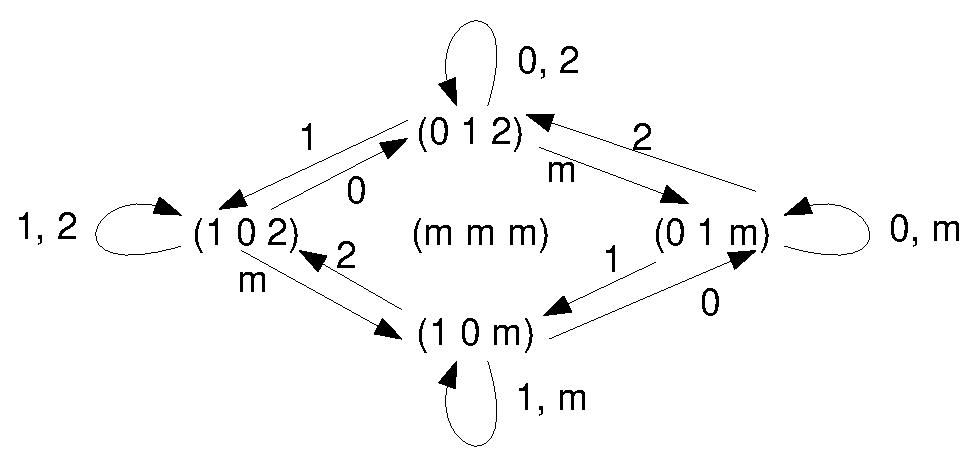
\includegraphics[width=0.7\textwidth]{2.theor/badpolicy}\\
  \caption{Граф для модельной стратегии вытеснения}\label{badpolicy}
\end{figure}

Для определения существования пути невытеснения может применяться
следующий алгоритм: сначала перебираются порядки на множестве чисел
$\{0, 1, ..., w{-}1\}$; обозначим очередной порядок как $i_1, i_2,
..., i_w$; строим множество вершин графа $V_1$, достижимых из (0~1
... $w{-}1$) по путям только с пометками $m$, в которых не встречается вершина ($m$ $m$ ... $m$); если среди таких путей есть путь с циклом,
алгоритм завершается с ответом <<путь невытеснения есть>>; иначе
строим множество вершин $V'_1$, достижимых из $V_1$ по дугам с
пометкой $i_1$; затем строим множество вершин графа $V_2$, достижимых из
вершин $V'_1$ по путям только с пометками $m$, в которых не встречается вершина ($m$ $m$ ... $m$); если среди таких путей есть путь с циклом,
алгоритм завершается с ответом <<путь невытеснения есть>>; иначе
строим множество вершин $V'_2$, достижимых из $V_2$ по дугам с
пометкой $i_2$; и так далее. Если путь с циклом нигде не встретился и все
возможные порядки просмотрены, алгоритм завершается с ответом <<пути
невытеснения нет>>.

В примере для модельной стратегии вытеснения, выбрав $i_1 = 0$, $i_2 = 1$, $i_3 = 2$, получим $V_1 = \{ (0~1~2), (0~1~m) \}$ и имеется путь с циклом: $m$ $m$ ..., в котором не встречается вершина ($m$ $m$ $m$). Тем самым путь невытеснения найден.

Граф для стратегий вытеснения \LRU и \PseudoLRU в случае\\двух-ассоциативной таблицы (для сокращения пометки заменены
штриховкой: дуга с пометка $m$ обозначена сплошной линией, дуга с
пометкой $0$ обозначена линией из точек, дуга с пометкой $1$
обозначена линией из пунктиров) изображен на
рисунке~\ref{fig:lrupolicy}. В этом графе есть всего один цикл,
состоящий из сплошных дуг -- петля на вершине ($m$ $m$). Поскольку он включает
в себя вершину ($m$ $m$), то в этом графе нет пути невытеснения.
В случае таблиц с б\'{о}льшим количеством строк в регионе ситуация будет
аналогичной.

Аналогичная ситуация будет и со стратегией вытеснения \FIFO (граф
для двух-ассоциативной таблицы изображен на рисунке~\ref{fig:fifopolicy}). В этом графе тоже всего один цикл, состоящий из сплошных дуг -- петля на вершине ($m$ $m$). Поскольку
этот цикл включает в себя вершину ($m$ $m$), то в этом графе нет
пути невытеснения. В случае буферов с большим количеством строк в регионе
ситуация будет аналогичной.

\begin{figure}[t]
\parbox{0.5\textwidth}{ \centering
  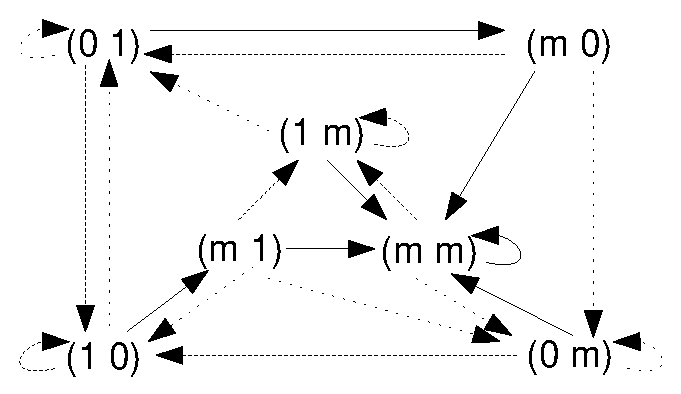
\includegraphics[width=0.45\textwidth]{2.theor/lrupolicy}
  \caption{Граф для стратегий вытеснения \LRU и \PseudoLRU с ассоциативностью 2}
  \label{fig:lrupolicy}
} \vline
\parbox{0.5\textwidth}{ \centering
  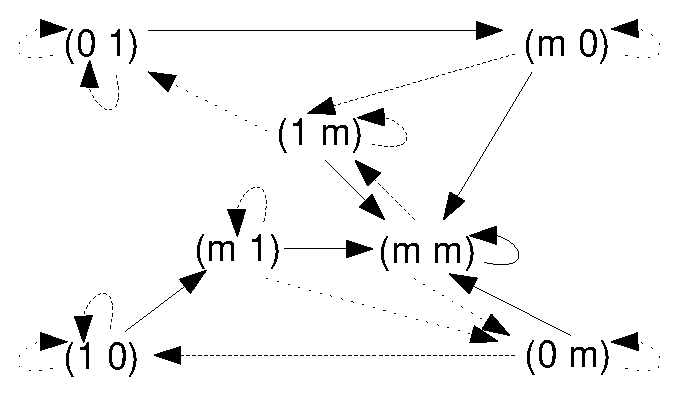
\includegraphics[width=0.45\textwidth]{2.theor/fifopolicy}
  \caption{Граф для стратегии вытеснения \FIFO с ассоциативностью 2}
  \label{fig:fifopolicy}
}
\end{figure}

%% надо ли общее доказательство для этих стратегий вытеснения ?

Предложенный орграф также полезен для получения верхней оценки количества инициализирующих обращений в таблицу (в алгоритме это число было названо $m$). Исходя из доказательства теоремы о полноте, можно сформулировать

\begin{utv}[Верхняя оценка количества инициализирующих обращений]
$$m \leqslant R \cdot (w + D)$$
где $R$ --- количество различных регионов, задействованных в тестовом шаблоне, $w$ --- ассоциативность таблицы (количество строк в регионе), $D$ --- максимальная длина ациклического пути в вершину ($m$ $m$ ... $m$) орграфа.
\end{utv}

$R$ --- есть атрибут тестового шаблона, $w$ --- атрибут структуры таблицы, $D$ --- атрибут функционирования таблицы.

Однако при рассмотрении конкретных случаев можно предложить и более сильные верхние оценки. Например, для стратегии вытеснения \LRU верна

\begin{theorem}[Верхняя оценка количества инициализирующих обращений для стратегии вытеснения
\LRU]\label{thm_mirror_lenth_lru} \UpperBoundLRUMirror
\end{theorem}
Доказательство теоремы приведено в приложении~\ref{proofs}.
\begin{sld}
      $$m = O(n)$$
\end{sld}

% доказать для алгоритмов теоремы корректности и полноты? что не теряются правильные решения и не появляются неправильные ?

\section{Конструирование тестовой программы для кэш-памяти первого и второго уровня}

В результате разрешения ограничений будет сгенерирована для каждой таблицы ключи и данные последовательности обращений. Как уже было сказано, задачей конструктора тестовых программ является построение инструкций микропроцессора, которые осуществляют вычисленные обращения. Для написания конструктора тестовых программ надо выяснить из документации по архитектуре способы исполнения инструкций, при которых задействованы различные таблицы. Если для таблицы нашлась инструкция, которая может произвести в нее обращение независимо от других таблиц, то эту инструкцию и будет использовать конструктор. Более сложный случай --- если такой инструкции найти не удается. В данном разделе будет показан один такой случай и возможное поведение конструктора тестовой программы для него.

Речь идет о кэш-памяти первого и второго уровня. Если обращение в кэш-память первого уровня оказывается успешным (попадание), то обращение в кэш-память второго уровня не производится. Получается, что последовательность обращений в кэш-память второго уровня влияет на последовательность обращений в кэш-память первого уровня: чтобы произошло обращение в кэш-память второго уровня, обращение в кэш-память первого уровня должно быть неуспешным; и, наоборот, при неуспешном обращении в кэш-память первого уровня возможно обращение в кэш-память второго уровня (которое может нарушить построенную инициализирующую последовательность для нее), правда, обращение к кэш-память второго уровня некоторые микропроцессоры позволяют запретить (например, микропроцессоры MIPS~\cite{MIPS64_III}). Но и это еще не всё: обращения в кэш-память обоих уровней осуществляются по одному и тому же адресу, тем самым для обращения в кэш-память второго уровня нужен промах обращения по специальному ключу в кэш-памяти первого уровня.

Поскольку инициализирующие последовательности ключей строятся в предположении произвольности состояния таблицы перед её выполнением и поскольку обращение в кэш-память второго уровня обязательно включает в себя обращение в кэш-память первого уровня, то в тестовой прогармме сначала надо инициализировать кэш-память второго уровня, а затем уже кэш-память первого уровня. Теперь надо понять, какую последовательность инструкций надо конструировать для инициализации каждого уровня кэш-памяти.

Еще раз вспомним, на основе чего надо проводить конструирование: каждый элемент инициализирующей последовательности --- это ключ, регион и, возможно, данные. Конструируются обычные инструкции, обычная программа на языке ассемблера. Но она должна осуществлять заданную последовательность обращений, в том числе, в кэш-память второго уровня. У каждой инструкции есть аргументы. Сконструировать программу --- значит выбрать последовательность названий инструкций и значения аргументов для них. Ключ и регион -- есть атрибуты адреса (физического или виртуального), который вычисляется по аргументам инструкции. Значит, ключ и регион нам даны, по ним надо собрать адрес, по адресу вычислить аргументы и, наконец, составить инструкцию из них.

\begin{figure}[h] \centering
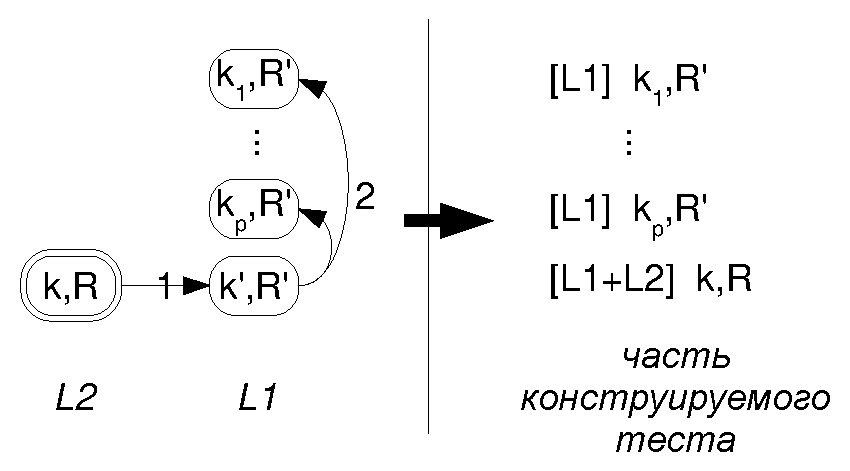
\includegraphics[width=0.6\textwidth]{2.theor/L1L2}
\caption{Конструирование обращения в кэш-память второго уровня вместе с обращениями в кэш-память первого уровня}\label{fig:L1L2}
\end{figure}

Итак, по последовательности ключей и регионов для кэш-памяти первого уровня инструкция составляется по только что приведенной схеме. С одним лишь уточнением, что адрес должен быть таким, что при обращении по нему кэш-память второго уровня не задействована. Теперь разберемся с последовательностью ключей и регионов для кэш-памяти второго уровня. Рисунок~\ref{fig:L1L2} схематически показывает, какие дополнительные инструкции можно строить для произвольного обращения по ключу $k$ в регион $R$ кэш-памяти второго уровня. А именно, ключу $k$ в регионе $R$ соответствует некоторый адрес, этому же адресу соответствуют и некоторый ключ $k'$ в регионе $R'$ кэш-памяти первого уровня (стрелка с цифрой 1). Но надо еще обеспечить отсутствие этого ключа, иначе обращения в кэш-память второго уровня не будет. Для этого надо сгенерировать небольшую последовательность произвольных различных и не равных $k'$ ключей $k_1, k_2, \dots, k_p$ и обратиться по ним в регион $R'$ кэш-памяти первого уровня без затрагивания кэш-памяти второго уровня (значение числа $p$ зависит от стратегии вытеснения).

%Рассмотрим один часто встречающийся случай кэширующих буферов,
%инициализация которого может вызывать трудности. Речь идет о
%кэш-памяти второго уровня. Зачастую кэш-память второго уровня не
%может быть инициализирована отдельно от остальных подсистем
%микропроцессора, обычно оно связано с изменением кэш-памяти первого
%уровня. Это создает дополнительные сложности при формулировании
%ограничений методом зеркальной генерации, поскольку инициализирующая
%последовательность должна подготавливать сразу два кэширующих буфера
%одновременно -- кэш-память первого уровня и кэш-память второго
%уровня. Кроме того, зачастую кэш-память второго уровня является
%совместной для хранения в ней данных и инструкций. Поэтому на
%инициализацию кэш-памяти второго уровня влияют и сами
%инициализирующие инструкции, и даже адрес расположения тестовой
%программы в памяти (от него зависит виртуальный адрес инструкций, а
%значит теги и индексы при обращении к кэш-памяти инструкций).
%
%Если принять дополнительное требование (и оно даст решение), что в
%кэш-памяти второго уровня наборы, используемые для доступа к
%инструкциям, не пересекаются с наборами, используемыми для доступа к
%данным, то генерируемые ограничения упрощаются (кэширование
%инструкций можно вообще не учитывать). С точки зрения зеркальной
%генерации это означает, что надо сформулировать требования на
%инициализирующую последовательность. Напомню, что одним из ключевых
%требований является произвольность начального состояния
%(содержимого) кэш-памяти.
%
%Предположим, что обращение к кэш-памяти второго уровня
%осуществляется при кэш-промахе в кэш-памяти первого уровня и
%кэш-память не является virtually indexed virtually
%tagged~\cite{HennessyPatterson3rd}. Для составления ограничений с
%использованием функций полезности необходимо знать, которые
%инструкции среди инициализирующей последовательности действительно
%обращаются в кэш-память второго уровня (иными словами, в каких
%инструкциях среди инициализирующей последовательности происходит
%кэш-промах при обращении к кэш-памяти первого уровня). Возможным
%решением было бы перебирать всевозможные распределения тестовых
%ситуаций в кэш-памяти первого уровня на элементах инициализирующей
%последовательности (с предварительной подготовкой этих тестовых
%ситуаций). Однако следующая лемма~\ref{special_initialization_L2}
%показывает, что для любого такого произвольного распределения
%тестовых ситуаций в кэш-памяти первого уровня существует решение со
%специальным распределением тестовых ситуаций. Это позволяет
%перебирать только такие специальные распределения тестовых ситуаций
%в кэш-памяти первого уровня. При этом вычислительная сложность
%процедуры поиска инициализирующей последовательности, дающей
%решение, изменяется от экспоненциальной от длины тестового шаблона к
%полиномиальной, что показывает лемма~\ref{max_k_h} (ее доказательство
%приведено в приложении~\ref{proofs}):
%\begin{lemma}[Верхняя оценка длины специальной инициализирующей
%последовательности для стратегии вытеснения \LRU]\label{max_k_h} \MaxUpperBoundLRU
%\end{lemma}
%\begin{sld}
%$$m = O(n)$$ где $m$ --- длина специальной инициализирующей
%последовательности, $n$ -- количество инструкций тестового шаблона.
%\end{sld}
%
%Для получения инициализирующей программы минимальной длины, можно
%применять сначала двоичный поиск суммы $k+h$ с применением
%дальнейшего поиска допустимых значений $k$ и $h$.


\chapter{Методы генерации ограничений для описания стратегий вытеснения}

\section{Свойство <<быть вытесненным>>}

Методы генерации ограничений из раздела ???????????? основываются на методах записи ограничения <<быть вытесненным>>. Иными словами, данный ключ <<вытеснен>> в таблице тогда и только тогда, когда в ней нет строки, которая бы подошла под этот ключ.

\begin{utv}\label{hit_miss_simpleform}
Пусть $L$ -- текущее множество строк таблицы, $(x,R)$ -- ключ и регион данного обращения. Тогда
\begin{itemize}
\item попадание выражается в виде ограничения $x \in L$ для региона $R$;
\item промах выражается в виде ограничения $x \notin L$ для региона $R$.
\end{itemize}
\end{utv}

Здесь и далее под ограничением <<$\in$>> будет пониматься наличие строки с подходящей <<ключевой частью>>. В том случае, когда в строке только одно поле ключа, принадлежность будет выражать естественным образом наличие или отсутствие строки. Кроме того, далее без ограничения общности речь будет вестись про произвольный регион (без явного введения переменных для региона).

Далее будет показано, как выразить свойство <<быть вытесненным>> с использованием дополнительных переменных, отвечающих вытесняемым строкам (они будут помечаться штрихованным способом).

Для переменной $L$ в каждой инструкции методом индукции может быть
составлено следующее выражение. База: $L$ для первой инструкции есть
начальное содержимое таблицы, это переменная величина в
системе уравнений. Теперь индуктивный шаг. Пусть выражение для
очередной инструкции $L$, а для следующей -- $LL$. Тогда если
обращение по ключу в очередной инструкции успешно (это попадание), то $LL
\equiv L$ (так как содержимое не меняется). Если это обращение неуспешно с
ключом $x$, то $LL \equiv (L \setminus \{x'\} \cup \{x\})$ в случае, если
в таблицу при промахе добавляются данные по требуемому ключу.
Для новой переменной $x'$ добавим в систему такие уравнения: $x' \in
L \wedge displaced_L(x')$. Предикат $displaced_L(x')$ истинен, если $x'$ является ключом вытесняемой строки при состоянии таблицы $L$. Предикат $displaced$ как раз и описывает
стратегию вытеснения.

Следующая теорема описывает выражение для $L$ без использования
индукции:
\begin{lemma}\label{L_current} \LcurrentBody
\end{lemma}
Доказательство леммы приведено в приложении~\ref{proofs}.

Например, если перед данной инструкцией располагается 3 инструкции с
промахами, то $L \equiv L_0 \setminus \{x'_1, x'_2, x'_3\} \cup
(\{x_1\} \setminus \{x'_2, x'_3\}) \cup (\{x_2\} \setminus \{x'_3\})
\cup \{x_3\}$.

\begin{theorem}[Дизъюнктивная форма уравнений для попаданий и промахов]\label{hit_miss_equations} \HitMissEquations
\end{theorem}
\begin{proof}
Применим утверждение~\ref{hit_miss_simpleform} и лемму~\ref{L_current} для записи текущего
состояния таблицы.

Для определения ключей вытесняемых строк добавляются ограничения:
\begin{itemize}
    \item такие, будто по этому ключу происходит попадание (поскольку вытесняемая строка
принадлежит текущему состоянию таблицы);
    \item $displaced(x')$ по определению вытесняемой строки.
\end{itemize}
\end{proof}

Заметьте, что получившиеся ограничения для попадания и
промаха получились очень похожими, хотя изначально вид ограничений у них был
совершенно противоположным.

Тем самым метод записи ограничения <<быть вытесненным>> сводится к методу записи ограничения $displaced$. Различие в них следующее: $displaced(x')$ истинен, если именно $x'$ является ключом строки, которая вытесняется именно в данной инструкции, а <<$x$ вытеснен>> истинно, если $x$ был вытеснен в одной из предыдущих инструкций и после этого не появлялся в таблице.

%Теорему~\ref{hit_miss_equations} можно переформулировать без
%использования вытеснямых тегов:
%
%\begin{utv}\label{hit_miss_human} Пусть $L_0$ -- множество
%адресов данных, расположенных в кэширующем буфере перед исполнением
%первой инструкции тестового шаблона. Тогда
%\begin{itemize}
%\item для инструкции с кэш-попаданием адреса $x$ следует добавить
%следующую совокупность уравнений:
%$$
%\left[
%   \begin{array}{l}
%    x \in L_0 \wedge x~\mbox{все еще не вытеснен} \\
%    x~\mbox{внесен одним из кэш-промахов} \wedge \mbox{с тех пор не вытеснен} \\
%   \end{array}
%  \right.
%$$
%
%\item для инструкции с кэш-промахом адреса $x$ следует добавить следующую систему
%уравнений ($\{x_i\}$ -- множество адресов данных в инструкциях с
%кэш-промахами, расположенными до текущей инструкции):
%$$
%\left[
%   \begin{array}{l}
%    x \notin L_0 \wedge x \notin \{x_1, x_2, ..., x_n\} \\
%    x~\mbox{был вытеснен} \wedge \mbox{не был больше внесен в буфер}\\
%  \end{array}
%\right.
%$$
%
%\end{itemize}
%\end{utv}
%
%Формально показано, что утверждение~\ref{hit_miss_human} описывает
%все возможные сценарии появления и вытеснения данных в кэширующих
%буферах. Однако применение этих ограничений в данном виде для
%реальных микропроцессоров может быть ограничено из-за большого
%размера $L_0$ (что влечет к большому размеру ограничений и к
%невозможности разрешения таких больших ограничений доступными
%инструментами). Далее будет показано, как \emph{совместное
%рассмотрение} тестовых ситуаций разных буферов и таблиц позволят
%существенно сократить размер этой формулы и обратиться к генерации
%ограничений для описания вытеснения.

Далее в этой главе даётся два метода генерации ограничений для описания стратегии вытеснения (описания свойства строки <<быть вытесненной>>): метод диапазонов вытеснения (ссылка?????????) и метод функций полезности (ссылка?????????). Поскольку методы предполагают анализ стратегии вытеснения, то перед их описанием (раздел~\ref{sec:plru_new_definition}) дан подробный комментарий о стратегии вытеснения \PseudoLRU, как мало исследованной в литературе по сравнению со стратегиями вытеснения \LRU и \FIFO. В разделе~\ref{sec:plru_new_definition} дается новое определение стратегии вытеснения \PseudoLRU, упрощающее применение предлагаемых методов.

В методе диапазонов вытеснения выражается предикат $displaced$ в виде ограничений, а в методе функций полезности свойство <<быть вытесненным>> выражается напрямую, без использования $displaced$.

Завершается глава разделом (ссылка????????????????) с частными случаями тестовых шаблонов и генерацией ограничений для этих случаев.

\section{Исследование стратегии вытеснения \PseudoLRU}\label{sec:plru_new_definition}

Стратегия вытеснения \LRU хоть и хорошо приближает поведение
таблицы к идеальному случаю (когда данные находятся в
таблице в тот момент, когда они нужны), однако все известные на
сегодняшний момент реализации \LRU для микропроцессоров требуют большого
количества дополнительной логики. Поэтому производятся поиски
стратегии вытеснения, близкой по эффективности к \LRU, но имеющей
реализацию с меньшими накладными расходами. Эти поиски привели к
стратегии вытеснения \PseudoLRU. Она используется в микропроцессорах архитектур PowerPC и Pentium~\cite{FundamentalOfComputerOrganizationAndDesign}.

\subsubsection{Каноническое определение \PseudoLRU на бинарном дереве}

Следующее описание часто встречается в
литературе~\cite{FundamentalOfComputerOrganizationAndDesign} при
определении \PseudoLRU. Оно формулируется на
упорядоченном бинарном дереве высоты $\log_2 w$, в листьях которого
подряд расположены строки (их количество равно $w$). Стратегия вытеснения \PseudoLRU
определяется только для таблиц с ассоциативностью, являющейся степенью двойки, поэтому число $\log_2 w$ является натуральным. Одна исходящая из вершины дуга помечена цифрой 0 (<<идущая налево>>), другая дуга помечена цифрой 1 (<<идущая направо>>). Вершины тоже помечаются цифрами 0 или 1. Стратегия вытеснения определяется как процесс изменения пометок в вершинах дерева.

При попадании <<в лист>> меняются пометки в нелистовых вершинах пути от корня до этого листа (см. рис.~\ref{pseudo_lru_hit}). А именно вершина получает пометку исходящей из нее дуги этого пути. Т.е. если дуга, соответствующая пути, выходит влево, вершина помечается цифрой 0, если вправо -- 1 (старая пометка вершины забывается). Пометки остальных вершин дерева не меняются.

\begin{figure}[h] \center
  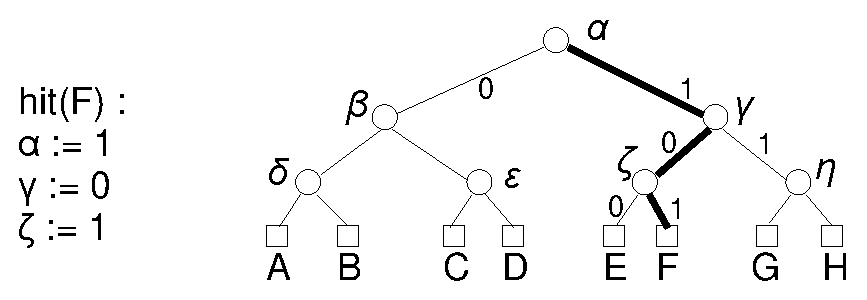
\includegraphics[width=0.7\textwidth]{2.theor/plruhit}\\
  \caption{Попадание для стратегия вытеснения \PseudoLRU
  (16-ассоциативная таблица)}\label{pseudo_lru_hit}
\end{figure}

На основании пометок вершин определяется и лист, по которому надо произвести вытеснение.
%Вытесняющий тег помещается в дереве на место вытесняемого.
Из корня дерева строится <<вытесняющий путь>> (он будет единственным), вытесняться будут данные листа этого пути. В <<вытесняющем пути>> нужная исходящая дуга каждой очередной вершины должна иметь пометку, противоположную пометке этой вершины. Т.е. если вершина помечена цифрой 0, значит дуга пути из этой вершины идет вправо, если вершина помечена цифрой 1 -- влево. Затем пометки вершин дерева изменяются так, как будто происходит попадание на <<вытесняемый>> лист. Пример того, как определяется вытесняемый элемент, показан на рис.~\ref{pseudo_lru_miss}. Цветом показаны пометки нелистовых вершин: черным вершинам соответствует пометка 1, белым
-- 0. В изображенном на рисунке дереве в качестве вытесняемого листа будет выбран D, к которому ведет путь $\alpha-\beta-\varepsilon$.

\begin{figure}[h] \center
  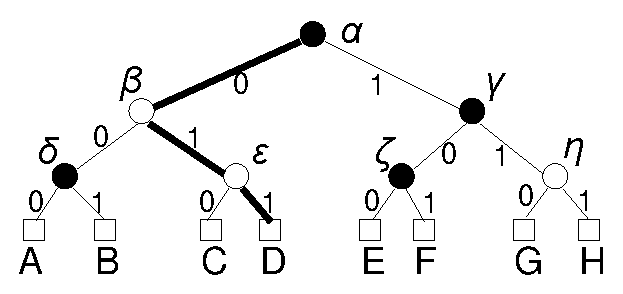
\includegraphics[width=0.5\textwidth]{2.theor/plrumiss}\\
  \caption{Определение вытесняемого элемента для стратегия вытеснения
  \PseudoLRU (16-ассоциативный кэширующий буфер)}\label{pseudo_lru_miss}
\end{figure}


\subsubsection{Каноническое определение \PseudoLRU на битовой строке}

Для каждого региона хранится битовая строка $\beta$ длины $w-1$, где $w$ --
ассоциативность таблицы. Стратегия вытеснения определяется как процесс изменения бит этой битовой строки.

Во многих книгах приводятся следующее определение стратегии
вытеснения \PseudoLRU для случая
$w=4$~\cite{FundamentalOfComputerOrganizationAndDesign} (в этом
случае для каждого региона выделяется 3 бита $B_1$, $B_2$ и $B_3$):
$$ \left[
  \begin{array}{c|ccc}
          & B_1 & B_2 & B_3 \\ \hline
    \pi_0 & 0 & 0 & \textsf{X} \\
    \pi_1 & 0 & 1 & \textsf{X} \\
    \pi_2 & 1 & \textsf{X} & 0 \\
    \pi_3 & 1 & \textsf{X} & 1 \\
  \end{array}
\right]
$$

Строки в регионе пронумерованы числами от 0 до $w-1$. При попадании на строку региона с номером $i$ задейстована строка матрицы, начинающаяся с $\pi_i$. Биты $\beta$, напротив которых в строке матрицы находится \textsf{X}, не меняются. Биты $\beta$, напротив которых в $i$'й строке находится число, принимают значение, равное этому числу.

При промахе надо определить номер вытесняемой строки. Для этого используется инвертированная форма той же матрицы:
$$
\left[
  \begin{array}{ccc|c}
    B_1 & B_2 & B_3 & \\ \hline
    1 & 1 & \textsf{X} & \rightarrow \pi_0 \\
    1 & 0 & \textsf{X} & \rightarrow \pi_1 \\
    0 & \textsf{X} & 1 & \rightarrow \pi_2 \\
    0 & \textsf{X} & 0 & \rightarrow \pi_3 \\
  \end{array}
\right]
$$

Выбирается строка, соответствующая текущему состоянию бит $B_1$,
$B_2$ и $B_3$: если напротив бита в строке находится число, бит
должен быть равен этому числу -- если напротив бита в строке
находится \textsf{X}, то требования на соответствующий бит нет.
Подходящая строка всегда будет существовать и она будет
единственной.

Изменение $\beta$ можно демонстрировать на бинарном дереве и
наоборот. $\beta$ составляется из пометок вершин дерева,
начиная с корня и далее по слоям от левых к правым вершинам (см.
рис.~\ref{plru_bittree}).

\begin{figure}[h] \center
  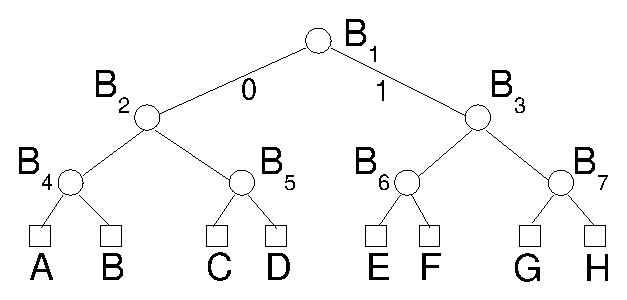
\includegraphics[width=0.5\textwidth]{1.review/plru}\\
  \caption{Битовая строка в бинарном дереве}\label{plru_bittree}
\end{figure}

Формализованное описание для всех допустимых $w$ в литературе не
приводится. Однако в дальнейшем для формулирования и доказательства
утверждений про стратегию вытеснения \PseudoLRU такое описание будет
необходимо. Для $w=8$ стратегия будет задаваться следующей матрицей:
$$
\left[
  \begin{array}{c|ccccccc}
          & B_1 & B_2 & B_3 & B_4 & B_5 & B_6 & B_7 \\ \hline
    \pi_0 & 0 & 0 & \textsf{X} & 0 & \textsf{X} & \textsf{X} & \textsf{X} \\
    \pi_1 & 0 & 0 & \textsf{X} & 1 & \textsf{X} & \textsf{X} & \textsf{X} \\
    \pi_2 & 0 & 1 & \textsf{X} & \textsf{X} & 0 & \textsf{X} & \textsf{X} \\
    \pi_3 & 0 & 1 & \textsf{X} & \textsf{X} & 1 & \textsf{X} & \textsf{X} \\
    \pi_4 & 1 & \textsf{X} & 0 & \textsf{X} & \textsf{X} & 0 & \textsf{X} \\
    \pi_5 & 1 & \textsf{X} & 0 & \textsf{X} & \textsf{X} & 1 & \textsf{X} \\
    \pi_6 & 1 & \textsf{X} & 1 & \textsf{X} & \textsf{X} & \textsf{X} & 0 \\
    \pi_7 & 1 & \textsf{X} & 1 & \textsf{X} & \textsf{X} & \textsf{X} & 1 \\
  \end{array}
\right]
$$

Следующее утверждение~\ref{wMinus1PseudoLRU} дает алгоритм
преобразования списка бит\\ $B_1, B_2, ..., B_{w{-}1}$ в результате
обращения в таблицу. В его формулировке применяется двоичное
разложение. Биты разложения обозначаются последовательностью от
старших бит к младшим (т.е. список ($x_1~x_2~\dots~x_n$) обозначает
число $x_n + 2\cdot x_{n-1} + 4\cdot x_{n-2} + \dots + 2^n\cdot x_1$, $x_i \in \{0,
1\}$ для $i = 1, 2, \dots, n$). Например, 1 = (0 0 1), 6 = (1 1 0).

Везде далее символ $W$ будет обозначать $\log_2 w$. По определению
стратегии вытеснения \PseudoLRU $W$ будет натуральным числом.

\begin{utv}[$(w{-}1)$-представление стратегии вытеснения
\PseudoLRU]\label{wMinus1PseudoLRU}При попадании строки с позицией
$i = (i_1~i_2~\dots~i_W)$ происходит следующее изменение бит $B_1,
B_2, ..., B_{w{-}1}$:

\parbox{0.3\textwidth}{
  $$ \begin{array}{l}
  B_{k_1} := i_1 \\
  B_{k_2} := i_2 \\
  B_{k_3} := i_3 \\
  ...\\
  B_{k_W} := i_W \\
  \end{array}$$
} \vline
\parbox{0.7\textwidth}{
  $$ \begin{array}{l}
  k_1 = (1) \\
  k_2 = (1~i_1) \\
  k_3 = (1~i_1~i_2) \\
  ...\\
  k_W = (1~i_1~i_2~\dots~i_{W{-}1}) \\
  \end{array} $$
}
\\[1cm]

При промахе позиция вытеснения $i = (i_1~i_2~\dots~i_W)$ определяется
следующим образом:

\parbox{0.3\textwidth}{
  $$ \begin{array}{l}
  i_1 = \neg B_{k_1} \\
  i_2 = \neg B_{k_2} \\
  i_3 = \neg B_{k_3} \\
  ...\\
  i_W = \neg B_{k_W} \\
  \end{array}$$
} \vline
\parbox{0.7\textwidth}{
  $$ \begin{array}{l}
  k_1 = (1) \\
  k_2 = (1~\neg B_{k_1}) \\
  k_3 = (1~\neg B_{k_1}~\neg B_{k_2}) \\
  ...\\
  k_W = (1~\neg B_{k_1}~\neg B_{k_2}\dots\neg B_{k_{W{-}1}}) \\
  \end{array} $$
}
\\[0.5cm]

Кроме того при кэш-промахе после определения позиции $i$ делается
преобразование бит $B_1, B_2, ..., B_{w{-}1}$ так, как в случае
попадания на $\pi_i$.
\end{utv}

Нехитрые расчеты показывают, что это утверждение верно для $w$ = 4 и 8.

\subsubsection{Определение \PseudoLRU на ветвях бинарного
дерева}\label{sec:PseudoLRUonBranches}

Здесь будет показано, как из канонического определения \PseudoLRU
получить формулировку \PseudoLRU с точки зрения одной строки региона
(каноническое определение рассматривает весь набор целиком и
для него формулирует правила работы с последовательностью бит $B_1,
B_2, ..., B_{w{-}1}$). Это определение ранее не встречалось в
литературе.

Сначала этот переход покажем на примере $w=4$. Первый шаг --- это
смена <<состояния>>: вместо последовательности бит $B_1, B_2, ...,
B_{w-1}$ будем рассматривать последовательность векторов бит
$\beta_0, \beta_1, \dots, \beta_{w-1}$ размера $W$. Каждый $\beta_i$
соответствует $i$'й листовой вершине бинарного дерева. Попадание
меняет теперь атрибуты не внутренних вершин дерева, а листовых.
Каждый $\beta_i$ будет представляться списком длины $W$ -- путь от
корня дерева к $i$'й листовой вершине: $\beta_0$ соответствует
($B_1$ $B_2$), $\beta_1$ соответствует ($B_1$ $\neg B_2$), $\beta_2$
соответствует ($\neg B_1$ $B_3$) и $\beta_3$ соответствует ($\neg
B_1$ $ \neg B_3$).\\[0.5cm]

\parbox{0.2\textwidth}{ \centering
  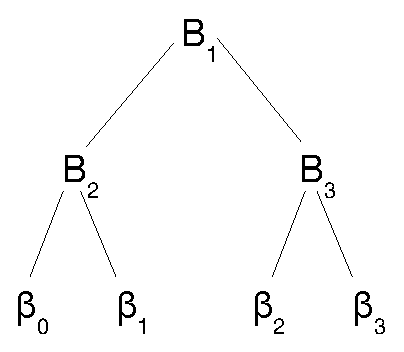
\includegraphics[width=0.2\textwidth]{1.review/btree}
}
\parbox{0.25\textwidth}{
$$ \left[
  \begin{array}{c|ccc}
          & B_1 & B_2 & B_3 \\ \hline
    \pi_0 & 0 & 0 & \textsf{X} \\
    \pi_1 & 0 & 1 & \textsf{X} \\
    \pi_2 & 1 & \textsf{X} & 0 \\
    \pi_3 & 1 & \textsf{X} & 1 \\
  \end{array}
\right]
$$
} $\stackrel{1}{\longrightarrow}$ %\vline
\parbox{0.4\textwidth}{
$$ \left[
  \begin{array}{c|cccc}
          & \beta_0 & \beta_1 & \beta_2 & \beta_3 \\ \hline
    \pi_0 & (0~0) & (0~1) & (1~\textsf{X}) & (1~\textsf{X}) \\
    \pi_1 & (0~1) & (0~0) & (1~\textsf{X}) & (1~\textsf{X}) \\
    \pi_2 & (1~\textsf{X}) & (1~\textsf{X}) & (0~0) & (0~1) \\
    \pi_3 & (1~\textsf{X}) & (1~\textsf{X}) & (0~1) & (0~0) \\
  \end{array}
\right]
$$
}

Заметим, что получилась симметричная матрица. На пересечении $\pi_i$
и $\beta_j$ располагается вектор, задающий изменение вектора в $j$'й
листовой вершине дерева при попадании $i$'й листовой вершины
дерева. Назовем позицию $i \oplus j$ \emph{относительной позицией}
$i$ относительно $j$. Рассмотрим отдельно каждый столбец
получившейся матрицы и переставим элементы столбца в порядке
увеличения относительных позиций.

\parbox{0.2\textwidth}{
$$ \left[
  \begin{array}{c|c}
          & \beta_0 \\ \hline
    \pi_0 & (0~0) \\
    \pi_1 & (0~1) \\
    \pi_2 & (1~\textsf{X}) \\
    \pi_3 & (1~\textsf{X}) \\
  \end{array}
\right]
$$
}\parbox{0.2\textwidth}{
$$ \left[
  \begin{array}{c|c}
          & \beta_1 \\ \hline
    \pi_0 & (0~1) \\
    \pi_1 & (0~0) \\
    \pi_2 & (1~\textsf{X}) \\
    \pi_3 & (1~\textsf{X}) \\
  \end{array}
\right]
$$
}\parbox{0.2\textwidth}{
$$ \left[
  \begin{array}{c|c}
          & \beta_2 \\ \hline
    \pi_0 & (1~\textsf{X}) \\
    \pi_1 & (1~\textsf{X}) \\
    \pi_2 & (0~0) \\
    \pi_3 & (0~1) \\
  \end{array}
\right]
$$
}\parbox{0.2\textwidth}{
$$ \left[
  \begin{array}{c|c}
          & \beta_3 \\ \hline
    \pi_0 & (1~\textsf{X}) \\
    \pi_1 & (1~\textsf{X}) \\
    \pi_2 & (0~1) \\
    \pi_3 & (0~0) \\
  \end{array}
\right]
$$
} $\stackrel{2}{\stackrel{\longrightarrow}{\pi^i_j \equiv \pi_{i
\oplus j}}}$

\parbox{0.24\textwidth}{
$$ \left[
  \begin{array}{c|c}
          & \beta_0 \\ \hline
    \pi^0_0 \equiv \pi_0 & (0~0) \\
    \pi^0_1 \equiv \pi_1 & (0~1) \\
    \pi^0_2 \equiv \pi_2 & (1~\textsf{X}) \\
    \pi^0_3 \equiv \pi_3 & (1~\textsf{X}) \\
  \end{array}
\right]
$$
}\parbox{0.24\textwidth}{
$$ \left[
  \begin{array}{c|c}
          & \beta_1 \\ \hline
    \pi^1_0 \equiv \pi_1 & (0~0) \\
    \pi^1_1 \equiv \pi_0 & (0~1) \\
    \pi^1_2 \equiv \pi_3 & (1~\textsf{X}) \\
    \pi^1_3 \equiv \pi_2 & (1~\textsf{X}) \\
  \end{array}
\right]
$$
}\parbox{0.24\textwidth}{
$$ \left[
  \begin{array}{c|c}
          & \beta_2 \\ \hline
    \pi^2_0 \equiv \pi_2 & (0~0) \\
    \pi^2_1 \equiv \pi_3 & (0~1) \\
    \pi^2_2 \equiv \pi_0 & (1~\textsf{X}) \\
    \pi^2_3 \equiv \pi_1 & (1~\textsf{X}) \\
  \end{array}
\right]
$$
}\parbox{0.24\textwidth}{
$$ \left[
  \begin{array}{c|c}
          & \beta_3 \\ \hline
    \pi^3_0 \equiv \pi_3 & (0~0) \\
    \pi^3_1 \equiv \pi_2 & (0~1) \\
    \pi^3_2 \equiv \pi_1 & (1~\textsf{X}) \\
    \pi^3_3 \equiv \pi_0 & (1~\textsf{X}) \\
  \end{array}
\right]
$$
}

После перехода к относительным позициям ($\pi^i_j$ -- это позиция
$\pi_j$ относительно $\pi_i$) все столбцы получились одинаковыми.
Иными словами, \emph{алгоритм изменения региона согласно стратегии
вытеснения \PseudoLRU на относительных позициях инвариантен
относительно абсолютной позиции вытесняемой строки}. Строка вытесняется в
том случае, когда её вектор равен (1 1). Следующая теорема
формально доказывает этот факт.

Будем называть \emph{\PseudoLRU-ветвью позиции $i$} вектор
$(B_{k_1}^{\sigma_1}~B_{k_2}^{\sigma_2}~\dots~B_{k_W}^{\sigma_W})$,
в котором $\sigma_j = \neg i_j$, $k_j = (1~i_1~i_2~\dots~i_{j-1})$,
$j = 1, 2, \dots, W$, $i = (i_1~i_2~\dots~i_W)$ (двоичное
разложение). Степени определены стандартным образом: $B^1 \equiv B,
B^0 \equiv \neg B$.

\begin{theorem}[Инвариантность преобразования \PseudoLRU-ветвей относительными
позициями]\label{thm_pseudoLRU_invariant} \PseudoLRUInvariant
\end{theorem}
Доказательство теоремы приведено в приложении~\ref{proofs}.

Доказанный факт позволяет сформулировать определение стратегии
вытеснения \PseudoLRU, сфокусированное не на изменении атрибутов строк всего региона,
а на изменении атрибутов одной строки. На этом определении
будут базироваться применения предлагаемых методов генерации
ограничений для стратегии вытеснения \PseudoLRU.

\begin{utv}[формулировка \PseudoLRU на ветвях бинарного дерева]
Сопоставим строке вектор длины $W$. Каждая инструкция, обращающаяся к этой строке,
делает её вектор равным (0 0 ... 0). Строка является вытесняемой в
том и только в том случае, если её вектор равен (1 1 ... 1).
Влияние других инструкций определяется относительной позицией их
строки относительно позиции данной строки. Если относительная позиция
принадлежит области $[\frac{w}{2^k},~\frac{w}{2^{k-1}}), k =
1,2,...,W$, то первые $k{-}1$ элементов вектора становятся равными
0, $k$'й элемент вектора становится равным 1, остальные элементы
вектора не меняются.
\end{utv}

Вектор длины $W$ будет соответствовать пути из корня бинарного
дерева в листовую вершину, соответствующую данной строке.
Будем называть процесс изменения элемента вектора
\emph{перекрашиванием вершины ветви}. Элементы вектора, равные 0,
будем называть \emph{белыми}, элементы вектора, равные 1, будем
называть \emph{черными}.

Говоря в терминах бинарного дерева, нелистовая вершина в ветви к
данной листовой вершине будет <<белой>>, если дуга пути от нее идет
налево и она помечена цифрой 1 или дуга пути от нее идет направо и она
помечена цифрой 0 (т.е. в том случае, когда направление дуги из нее
соответствует пометке этой дуги). Нелистовая вершина будет
называться <<черной>>, если направление дуги пути из нее не соответствует
пометке этой дуги. Вытесняется та строка, путь к которой
полностью состоит из несоответствующих дуг. На рисунке~\ref{recolor}
изображен процесс перекрашивания ветви, ведущей в А, под действием
попадания в C (для сокращения показана только ветвь в А без
остальной части дерева). Так как путь из корня в C совпадает из
верхних двух вершин, то они перекрашиваются в белый цвет. Дуга из
третьей вершины пути в С не совпадает с дугой пути в А, поэтому
третья вершина перекрашивается в черный цвет. Остальные вершины
ветви остаются без изменений.

\begin{figure}[h] \center
  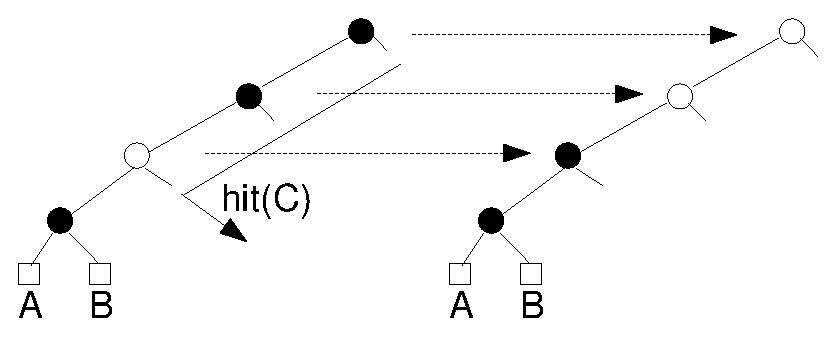
\includegraphics[width=0.8\textwidth]{1.review/recolor}\\
  \caption{Перекрашивание ветви в А}\label{recolor}
\end{figure}


Определение стратегии вытеснения \PseudoLRU на ветвях дерева
является связующим звеном между каноническим определением (например,
на битовой строке) и определением с помощью таблицы вытеснения,
поскольку ветвь -- это и есть позиция, которая меняется точно так
же, как и позиция в перестановке согласно таблице вытеснения.

\section{Метод перебора диапазонов вытеснения записи стратегии
вытеснения в виде ограничений}

{\footnotesize В разделе рассматривается метод составления ограничений, описывающих
стратегию вытеснения. Метод применяется к стратегиям вытеснения, для
которых можно определить \emph{метрику вытеснения} и \emph{диапазон
вытеснения}. Составляемые ограничения представляют собой дизъюнкции
по всем возможным диапазонам вытеснения для данного вытесняемого
тега. В разделе приведены метрики вытеснения и ограничения для трех
наиболее часто использующихся в микропроцессорах стратегий
вытеснения --- \LRU, \FIFO и \PseudoLRU}.

Неформально говоря, \emph{диапазон вытеснения} -- это непрерывная
часть тестового шаблона, заканчивающаяся в данной инструкции (это
т.н. \emph{конец диапазона вытеснения}). Эта непрерывная часть непосредственно
влияет на вытеснение строки конца диапазона.
Зачастую \emph{началом диапазона вытеснения} является инструкция, в
которой осуществляется последнее обращение к этой строке.

\emph{Метрикой вытеснения} будем называть функцию от текущего
состояния таблицы и части тестового шаблона. Она
максимальна в конце диапазона вытеснения и минимальна в начале
диапазона вытеснения.

Метод заключается в выделении метрики вытеснения, затем в выделении диапазона вытеснения и, наконец, выписывании ограничений (constraints), выражающих определение данного диапазона вытеснения.

\subsection{Метод перебора диапазонов вытеснения для стратегии
вытеснения \LRU}\label{sec:LRU_constraints}

\LRU (Least Recently Used) --- это стратегия вытеснения,
определяющая вытесняемые данные как наименее используемые. Она
эффективна для алгоритмов, обладающих свойством локальности данных,
т.е. чаще использующих те данные, к которым недавно происходило
обращение. Эта стратегия используется, например, в микропроцессорах
архитектуры MIPS~\cite{mips64_II}.

Стратегия вытеснения \LRU обычно определяется с использованием
счетчиков обращений. Для каждой строки таблицы
вводится счетчик обращений к ней. Каждое обращение увеличивает
счетчик. Вытесняемым в регионе будет элемент с минимальным счетчиком его строк.
Поскольку границы значений счетчика неизвестны, формулирование
метрики вытеснения на основе счетчика провести сложно.

Другой способ описания \LRU основан на введении порядка на строках региона (т.е. регион представляется списком строк). После каждой
инструкции элементы этого списка переупорядочиваются согласно следующим правилам
(см.рис.~\ref{fig:lru1}):
\begin{itemize}
\item при попадании элемент, соответствующий адресу инструкции,
перемещается в начало, остальные элементы от первого до данного
сдвигаются на одну позицию;
\item при промахе вытесняется последний элемент, в начало
вставляется элемент, вызвавший промах.
\end{itemize}

\begin{figure}[h] \center
  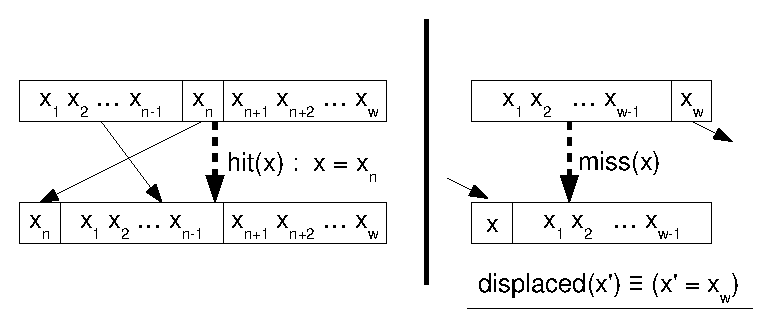
\includegraphics[width=0.6\textwidth]{2.theor/lru1}\\
  \caption{Стратегия вытеснения \LRU (w --- ассоциативность) на списках}\label{fig:lru1}
\end{figure}

Это описание подходит для определения метрики вытеснения: ею будет
\emph{индекс элемента в этом списке}. Такая метрика максимальна в
момент вытеснения (индекс равен длине списка). Значит, минимальное значение
она принимает в момент попадания на этот элемент (т.к. он
переносится в самое начало, индекс становится равным 1). Значит,
применение перебора диапазонов вытеснения возможно (выделена метрика
вытеснения), началом диапазонов вытеснения будет последнее обращение
к вытесняемому элементу.

\begin{utv}[метрика вытеснения для стратегии вытеснения \LRU]
Метрикой вытеснения элемента для стратегии вытеснения \LRU является
индекс элемента в наборе согласно порядку последних обращений.
Диапазон вытеснения начинается в инструкции, последний раз
обращающейся к элементу (или в начальном состоянии, если инструкции
тестового шаблона к этому элементу не обращаются).
\end{utv}

Другое объяснение таким диапазонам вытеснения можно дать, исходя из
самого определения \LRU. А именно, если элемент должен стать \LRU,
т.е. наиболее неиспользуемым, все остальные элементы, наоборот,
должны быть хотя бы раз использованы (т.е. к ним должны быть
обращения до вытесняющей инструкции). Иными словами, чтобы элемент
был вытеснен, необходимо и достаточно, чтобы между последним
обращением к нему и вытеснением были обращения ко всем элементам
текущего состояния кэширующего буфера, кроме него (см.
рис.~\ref{lru-ranges}).

\begin{figure}[h] \center
  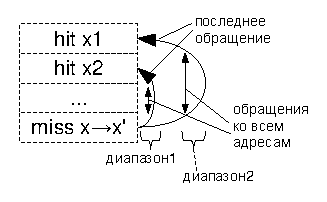
\includegraphics[width=0.4\textwidth]{2.theor/lru}\\
  \caption{Диапазоны вытеснения для стратегии вытеснения \LRU}\label{lru-ranges}
\end{figure}

Запишем в виде уравнений на множества эту логику~\cite{my_syrcose_2009}. Предикат\\
$displaced(x')$ будет представлен дизъюнкцией уравнений --- каждый
элемент дизъюнкции соответствует некоторому диапазону вытеснения.
Тогда для диапазона вытеснения к инструкции, обращающейся по ключу
$y$ надо составить такую систему уравнений ($x_1, x_2, ..., x_n$ --
ключи, по которым происходят обращения внутри диапазона
вытеснения, а также элементы начального состояния, если диапазон начинается там, $L$ --
выражение для состояния таблицы перед инструкцией, в которой вытесняется $x'$):
$$
\left\{
   \begin{array}{l}
    x' = y \\
    \{x_1, x_2, ..., x_n\} \cap R(y) = (L \setminus \{y\}) \cap R(y)\\
   \end{array}
  \right.
$$

Функциональный символ $R$ обозначает множество ключей того же региона. Он может быть определен формально следующим образом:
$$x_i \in R(x_k) \Leftrightarrow R_i = R_k$$
А именно ключ $x_i$ (с регионом $R_i$) принадлежит $R$ от ключа $x_k$ (с регионом $R_k$) тогда и только тогда, когда их регионы совпадают, т.е. $R_i = R_k$. Если вместо $x_i$ рассматривается элемент начального состояния, то $R_i$ --- это регион, в котором этот элемент находится.

Следующая теорема обосновывает и упрощает систему уравнений для $x'$.
\begin{theorem}[Уравнение для \LRU]\label{LRU_equation} \DiapazonLRU
\end{theorem}

Доказательство теоремы приведено в приложении~\ref{proofs}.

\subsection{Метод перебора диапазонов вытеснения для стратегии
вытеснения \FIFO}

\FIFO (First-In First-Out) -- это стратегия вытеснения, определяющая
вытесняемые данные согласно принципу очереди FIFO. Например, в
микропроцессоре PowerPC 970FX вытеснение из небольшого буфера,
хранящего последние преобразованные эффективные адреса в физические,
D-ERAT происходит согласно \FIFO~\cite{PowerPC970FXUserManual}.

Стратегия \FIFO может быть описана на основе порядка на строках
региона (т.е. регион представляется списком строк-элементов). После каждой
инструкции элементы переупорядочиваются согласно следующим правилам
(см.рис.~\ref{fifo1}):
\begin{itemize}
\item при попадании порядок элементов не меняется;
\item при промахе вытесняется последний элемент, в начало вставляется элемент, вызвавший промах.
\end{itemize}

\begin{figure}[h] \center
  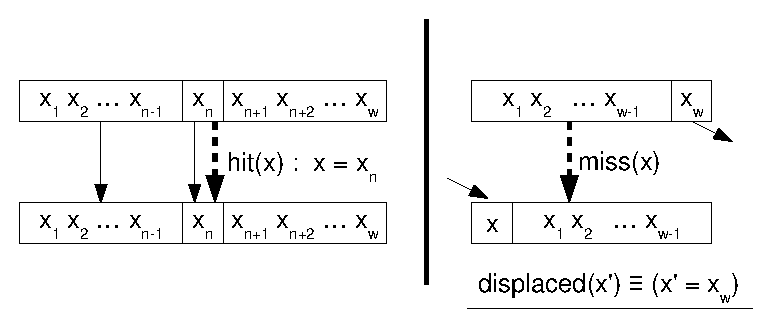
\includegraphics[width=0.6\textwidth]{2.theor/fifo1}\\
  \caption{Стратегия вытеснения \FIFO (w --- ассоциативность таблицы)}\label{fifo1}
\end{figure}

Отличие от \LRU лишь в том, что при \FIFO не происходит перестановки
элементов набора при возникновении попадания. Поэтому таблица
вытеснения~\cite{policy_tables} для стратегии вытеснения \FIFO будет
выглядеть так, как изображено на рисунке~\ref{fifo_policy_table}.

\begin{figure}
$$
  \left[
    \begin{array}{c|cccccc}
      \pi_0 & 0 & 1 & 2 & 3 & \dots & w-1 \\
      \pi_1 & 0 & 1 & 2 & 3 & \dots & w-1 \\
      \pi_2 & 0 & 1 & 2 & 3 & \dots & w-1 \\
      \vdots &  &  &  & & & \\
      \pi_{w-1} & 0 & 1 & 2 & 3 & \dots & w-1 \\
      \pi_m & m & 0 & 1 & 2 & \dots & w-2 \\
    \end{array}
  \right]
$$
\caption{Таблица вытеснения для \FIFO}\label{fifo_policy_table}
\end{figure}

Как и для \LRU, в качестве метрики вытеснения можно взять индекс
элемента в списке, что дает возможность использовать перебор
диапазонов вытеснения.
Началом диапазона вытеснения будет внесение элемента в кэширующий
буфер, концом диапазона вытеснения -- его вытеснение. При
составлении ограничений все инструкции с попаданиями внутри
диапазона будем игнорировать (они не влияют на вытеснение с точки
зрения \FIFO). Тогда \emph{\FIFO будет выполнено в том случае, когда
в диапазоне встречаются все строки таблицы без вытесняемой}.

\begin{utv}[метрика вытеснения для стратегии вытеснения \FIFO]
Метрикой вытеснения строки для стратегии вытеснения \FIFO является ее
индекс в наборе согласно порядку последних обращений. Диапазон
вытеснения начинается в инструкции c промахом, последний раз
обращающейся к вытесняемой строке (или в начальном состоянии, если
инструкции тестового шаблона к этоЙ строке не обращаются).
\end{utv}

Запишем в виде уравнений на множества эту логику~\cite{my_nivc_2009}. Предикат\\
$displaced(y')$ будет представлен дизъюнкцией уравнений -- каждый
элемент дизъюнкции соответствует некоторому диапазону вытеснения.
Тогда для диапазона вытеснения к инструкции, обращающейся к адресу
$y$, надо составить такую систему уравнений ($y_1, y_2, ..., y_n$ --
множество ключей, по которым происходят обращения внутри диапазона
вытеснения \textbf{с промахами}, а также элементы начального
состояния, если диапазон начинается там, $L$ -- выражение для
состояния таблицы для инструкции, вытесняющей $y'$):
\begin{theorem}[Уравнение для \FIFO]\label{FIFO_equation} \DiapazonFIFO
\end{theorem}

Функциональный символ $R$ используется в том же смысле, как он использовался для \LRU:  множество ключей того же региона. Доказательство теоремы приведено в приложении~\ref{proofs}.

\subsection{Метод перебора диапазонов вытеснения для стратегии
вытеснения \PseudoLRU}

Воспользуемся определением \PseudoLRU на ветвях бинарного дерева
(см. п.~\ref{PseudoLRUonBranches}). Согласно этому определению при
попадании (или внесении в таблицу) строки её ветвь
<<обнуляется>>, т.е. становится равной (0 0 ... 0). Каждая
последующая инструкция перекрашивает часть этой ветви до тех пор,
пока к некоторому промаху эта ветвь не станет равной (1 1 ...
1). В этом случае данная строка будет вытеснена. Таким образом, в
качестве метрики вытеснения предлагается использовать количество
единиц в ветви. Это количество максимально в момент вытеснения и
минимально в момент попадания (или внесения) по ней.
Применение перебора диапазонов вытеснения для описания \PseudoLRU
возможно: началом диапазона будет последнее обращение к строке
(листовой вершине дерева), концом диапазона будет вытесняющая эту строку инструкция.

\begin{utv}[метрика вытеснения для стратегии вытеснения \PseudoLRU]
Метрикой вытеснения элемента для стратегии вытеснения \PseudoLRU
является количество вершин в пути к вытесняемой листовой вершине с
пометками, противоположными пометкам при прохождении по пути при
попадании. Диапазон вытеснения начинается в инструкции,
последний раз обращающейся к листовой вершине (или в начальном
состоянии, если инструкции тестового шаблона к этой листовой вершине
не обращаются).
\end{utv}

%Отличием этой метрики вытеснения от метрики вытеснения для \LRU или
%\FIFO является \emph{немонотонность}. Обращение к листовым вершинам,
%лежащим близко к данной, может перекрасить в белый цвет некоторые до
%этого бывшие черными вершины, что уменьшит метрику, но не сделает ее
%значение минимальной. Как будет продемонстрировано ниже, монотонные
%метрики вытеснения позволяют строить более компактные ограничения,
%чем немонотонные. Метрика вытеснения не является единственной для
%стратегии вытеснения, поэтому поиск монотонной метрики вытеснения
%является еще одним способом упрощения ограничений.

Осталось записать уравнения, описывающие предложенные диапазоны
вытеснения. Обозначим позиции строк буквой $\pi$. Предикат $displaced(x')$ будет
представлен дизъюнкцией уравнений -- каждый элемент дизъюнкции
соответствует некоторому диапазону вытеснения. Тогда для диапазона
вытеснения к инструкции, обращающейся по ключу $x_1$ c позицией
$\pi_1$ надо составить такую систему уравнений (~$x_2, x_3, ...,
x_n$ -- множество ключей, к которым происходят обращения внутри
диапазона вытеснения, $\pi_2, \pi_3, ..., \pi_n$ -- соответствующие
им позиции, $\delta_i = \pi_i \oplus \pi', i = 2,3,\dots,n$, --
относительные позиции ):

\begin{figure}[h] \center
  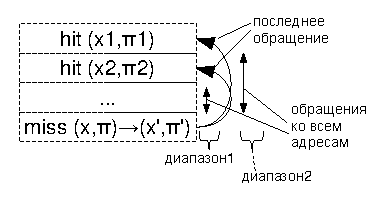
\includegraphics[width=0.5\textwidth]{2.theor/plru-ranges}\\
  \caption{Диапазоны вытеснения для стратегии вытеснения \PseudoLRU}
\end{figure}

$$
\left\{
\begin{array}{l}
x' = x_1\\
\pi' = \pi_1\\
\pi = \pi'\\
((0~op_x~\delta_2)~op_x~\delta_3) ... ~op_x~\delta_n  = w-1\\
\end{array}
\right.
$$

Операция $op_x$ выполняет очередной шаг по <<перекрашиванию>> пути,
ведущего в элемент $x$. Она может быть определена следующей формулой:

$$X~op_x~\delta \equiv \mbox{~if~} R(X) \neq R(x) \mbox{~then~} X \mbox{~else~} (X \&
\delta_{<1>}) | \delta_{<0>} \mbox{~end~}$$

где \& -- побитовая конъюнкция, | -- побитовая дизъюнкция,
$\delta_{<1>} = 2 * \delta_{<0>} - 1$, а $\delta_{<0>} = 2^{[\log_2
\delta]}$ может быть определено следующим переборным способом:
$\delta_{<0>} = \mbox{~if~} 1 \leqslant \delta < 2 \mbox{~then~} 1
\mbox{~elsif~} 2 \leqslant \delta < 4 \mbox{~then~} 2 \mbox{~elsif~}
... \mbox{~else~} w \mbox{~end~}$. Другой способ получения
$\delta_{<0>}$ и $\delta_{<1>}$ удобно применять при побитовом
рассмотрении $\delta$: $\delta_{<0>} = (\delta_{<1>} + 1) \gg 1$,
$\delta_{<1>}[i] = \delta[1] \vee \delta[2] \vee ... \vee
\delta[i]$, где символом $d[i]$ обозначен $i$'й бит числа $d$, биты
нумеруются со старших к младшим.


%%%%%%%%%%%%%%%%%%%%%%%%%%%%%%%%%%%%%%%%%%%%%%%%%%%%%%%%%%%%%%%%%%%%

\pagebreak
\section{Метод функций полезности записи стратегии вытеснения в виде
ограничений}\label{sec:usefulness_functions}

{\footnotesize В разделе рассматривается метод составления ограничений для описывания
стратегии вытеснения, для которой можно определить метрику
вытеснения. Стратегия вытеснения описывается ограничением сверху на
количество \emph{полезных} инструкций (т.е. помогающих вытеснению).
В разделе приведены метрики полезности и ограничения для трех
наиболее часто использующихся в микропроцессорах стратегий
вытеснения -- \LRU, \FIFO и \PseudoLRU. Освещается понятие
\emph{монотонной метрики вытеснения}, которая является залогом более
компактной системы ограничений.}

В данном разделе процесс вытеснения будет представляться как изменение значений системы функций, отображающих ключи в целые числа. Т.е. вводится набор функций, отображающий ключи в целые числа. Каждая инструкция изменяет значения функций по всем ключам. Для каждого отдельного ключа этот процесс можно представить графиком (см. рис.~\ref{fig:graphic}).

\begin{figure}[h] \center
  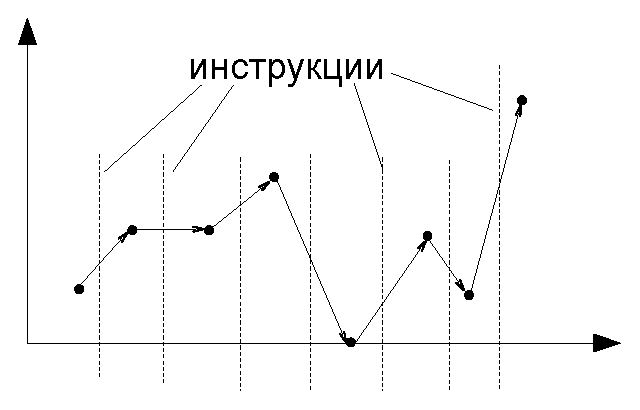
\includegraphics[width=0.5\textwidth]{2.theor/graphic}\\
  \caption{К определению стратегии вытеснения}\label{fig:graphic}
\end{figure}

Говоря формально, пусть $\alpha, \beta, \dots, \gamma$ --- одноместные функции, отображающие ключи в целые числа. Для каждой инструкции определены функции изменения значений функций $\alpha, \beta, \dots, \gamma$:
$$\parbox{2.5cm}{in-parallel\\forall x~}\left|\begin{array}{l}
\alpha(x) := A_I(k, \alpha, \beta, \dots, \gamma)\\
\beta(x) := B_I(k, \alpha, \beta, \dots, \gamma)\\
\dots\\
\gamma(x) := C_I(k, \alpha, \beta, \dots, \gamma)\\
\end{array}\right.
$$

Обновления $\alpha, \beta, \dots, \gamma$ выполняются одновременно. $I$ --- инструкция, $k$ --- ключ в этой инструкции. Функции $A_I$, $B_I$, \dots, $C_I$ отражают влияние обращения по некоторому ключу на другой произвольный ключ. Возможны следующие случаи (в качестве $x$ рассматривается произвольный ключ, не обязательно <<находящийся>> в регионе):
\begin{itemize}
    \item в результате обращения по ключу $k$ ключ $x$ <<попадает>> в регион (т.е. в регион добавляется строка с ключом $x$);
    \item в результате обращения по ключу $k$ ключ $x$ <<вытесняется>> из региона (т.е. из региона удаляется строка с ключом $x$);
    \item в результате обращения по ключу $k$ состояние ключа $x$ в регионе не меняется.
\end{itemize}

Этим ситуациям как раз и ставятся в соответствие классы значений функций $\alpha, \beta, \dots, \gamma$, а функции $A_I$, $B_I$, \dots, $C_I$ осуществляют переход между этими классами. Тем самым стратегия вытеснения будет описана в виде изменения таких <<счетчиков>> $\alpha, \beta, \dots, \gamma$.

Формально это правило можно выразить следующим образом. Будем называть функцию $\alpha$ \emph{метрикой вытеснения} для заданной стратегии вытеснения, если одновременно выполнены следующие свойства:
\begin{enumerate}
  \item существуют константы $\alpha_{min}$ и $\alpha_{max}$ такие, что $\alpha_{min} \leqslant \alpha_{max}$;
  \item для любого ключа $x$ $\alpha_{min} \leqslant \alpha(x) \leqslant \alpha_{max}$ тогда и только тогда, когда $x$ находится в регионе по определению стратегии вытеснения;
  \item для любого ключа $k$ $A_I(k, \alpha,\beta,\dots,\gamma) (k) = \alpha_{min}$;
  \item $\exists! \phi: \mbox{~ключ~}^2 \times \mathds{Z}^{2\cdot n} \rightarrow \mathds{Z}$, где $n$ --- количество функций во множестве $\{\alpha,\beta,\dots,\gamma\}$, такая, что для любого ключа $x$ $A_I(k, \alpha,\beta,\dots,\gamma)(x) \equiv \phi(k, \alpha(k), \beta(k), \dots, \gamma(k), x, \alpha(x), \beta(x), \dots, \gamma(x))$; иными словами, в функции изменения метрики вытеснения разрешается обращаться только к $k$ и тому ключу, для которого определяется метрика вытеснения;
  \item $\exists! x^* : \alpha(x^*) = \alpha_{max}$;
  \item перед любым неуспешным обращением (промахом) $\alpha(x^*) = \alpha_{max}$ тогда и только тогда, когда $x^*$ есть <<вытесняемый>> ключ по определению стратегии вытеснения (т.е. строка с ключом $x^*$ является вытесняемой при данном обращении по определению стратегии вытеснения);
\end{enumerate}

Пример метрики вытеснения: $\alpha$ --- счетчик количества обращений к строке для стратегии вытеснения \LRU. Обращение по тому же счетчику делает $\alpha$ равным 1, по другому ключу --- увеличивает $\alpha$ на единицу. Вытесняемым считается ключ, чей счетчик равен $w$ --- количеству строк в регионе. Проверим определение метрики вытеснения:
\begin{enumerate}
    \item $\alpha_{min}$ = 1, $\alpha_{max}$ = $w$, $1 \leqslant w$;
    \item верно, что счетчик больше $w$ тогда и только тогда, когда $x$ не находится в регионе; в противном случае, было бы возможно успешное обращение к большему числу строк, чем хранится в регионе;
    \item по условию обращение по тому же счетчику делает $\alpha$ равным 1, что и есть $A_I(x;...)(x) = 1$;
    \item изменение одного счетчика не требует изменения других счетчиков (т.е. они, конечно, изменяются, но все изменения счетчиков можно проводить независимо);
    \item такой $x^*$ существует, ибо в противном случае было бы возможно успешное обращение к большему числу строк, чем хранится в регионе; такой $x^*$ единственный, поскольку каждая инструкция меняет каждый счетчик и в минимальное значение $\alpha$ изменяется лишь по единственному ключу.
\end{enumerate}

Пусть для стратегии вытеснения сформулирована метрика вытеснения. Будем называть
инструкцию (обращение по некоторому ключу) \emph{полезной для вытеснения} ключа $x$ (или просто, \emph{полезной}), если она увеличивает метрику вытеснения по ключу $x$ на этапе монотонного увеличения метрики до максимального значения (см.
рис.~\ref{useful}).

\begin{figure}[h] \center
  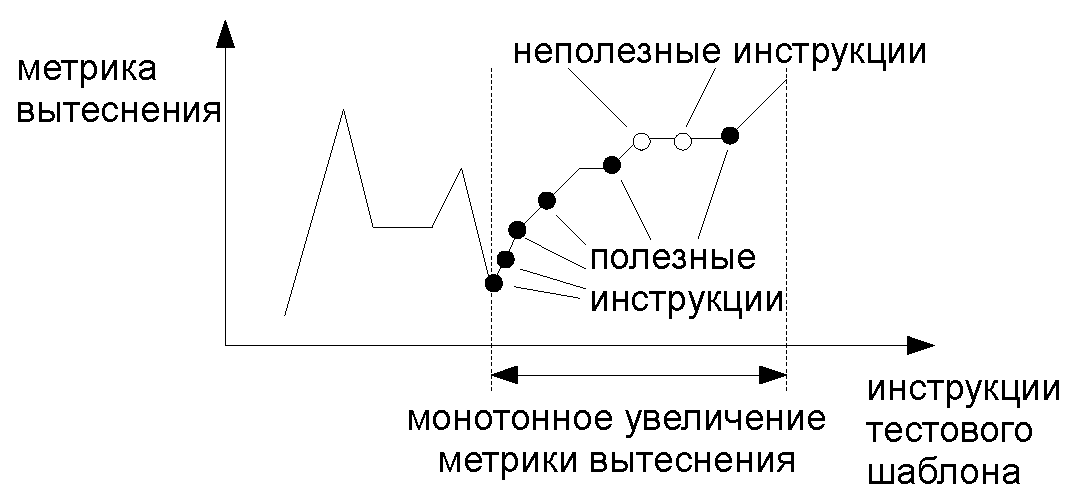
\includegraphics[width=0.6\textwidth]{2.theor/useful}\\
  \caption{К определению полезных инструкций}\label{useful}
\end{figure}

Тогда вытеснение будет происходить в том случае, когда количество
полезных инструкций превысит некоторое константное количество.
И вытеснение не будет происходить, если количество полезных инструкций
не превысит некоторой константной верхней границы.

\emph{Функцией полезности} инструкции будем называть характеристическую функцию свойства инструкции быть полезной. Т.е. функция полезности для полезной инструкции равна 1, для остальных инструкций равна 0. В дальнейших формулировках функцией полезности могут обозначаться просто предикаты, что надо воспринимать как функцию, равную 1 при истинном предикате и 0 при ложном.

Тем самым ограничение (constraint) <<быть вытесненным>> можно представить в виде ограничения сверху на сумму функций полезности инструкций, составляющих тестовый шаблон: $\sum_{i=1}^n u_x(k_i) < N$, где $u_x(k_i)$ -- функция полезности обращения по ключу $k_i$ для ключа $x$. Если будет важен регион, в который происходит обращение, то он также будет указываться: $u_{x,r}(k_i, r_i)$. Еще раз подчеркну, что представленное неравенство выражает ограничение количества полезных инструкций, каждая полезная инструкция увеличивает метрику вытеснения, значит при должном количестве полезных инструкцкий метрика вытеснения примет <<максимальное>> значение ($\alpha_{max}$) и произойдет вытеснение.

Функции полезности, как и метрики вытеснения, не являются единственными. Например, для стратегии вытеснения \LRU возможны следующие две различные функции полезности (далее для одной из них будет формально показано, что она действительно является функцией полезности) (функции вытеснения приведены для случая полностью ассоциативной таблицы):
\begin{itemize}
  \item $u_x(x_i) \equiv (x \notin \{x_i, x_{i+1}, ..., x_n\} \wedge \bigwedge\limits_{j=1,2,...,i-1} (x \in \{x_j, x_{j+1}, ..., x_{i-1}\} \vee x_j \neq x_i))$ -- инструкция считается полезной, если она расположена после последнего обращения к $x$ и с того момента является первым обращением к своему ключу; тут можно вспомнить определение \LRU на рисунке~\ref{fig:lru1}, где обращение по ключу $x_j$, который расположен после ключа $x$, передвигает $x$ к концу списка, на котором происходит вытеснение; первые обращения по ключам после последнего обращения к $x$ -- это и есть именно те обращения, где $x$ сдвигается к концу; иначе говоря, полезная инструкция сдвигает $x$ к концу, приближая его к вытеснению;
  \item $u_x(x_i) \equiv (x \notin \{x_i, x_{i+1}, ..., x_n\} \wedge x_i \notin \{x_{i+1}, x_{i+2}, ..., x_n\})$ -- инструкция считается полезной, если она расположена после последнего обращения к $x$ и является последним обращением к своему ключу перед финальным обращением к $x$; т.е. в таблице хранятся некоторые ключи, есть некоторый ключ $x$, есть последовательность других обращений (их ключи есть $x_i$, ..., $x_n$), полезными будут лишь последние к ним обращения (среди $x_i$, ..., $x_n$ могут быть равные), т.е. все полезные инструкции вместе образуют (по разу) все различные ключи (ровно это же говорит и уравнение для \LRU -- см. теорему~\ref{LRU_equation}).
\end{itemize}

Тем самым, метод функций полезности состоит в следующем:
\begin{enumerate}
  \item выделить метрику вытеснения $\alpha$;
  \item выделить определение полезной инструкции;
  \item записать функцию полезности $u_{x,r}(x_i, r_i)$ для инструкции с ключом $x$ и регионом $r$;
  \item определить $\alpha_{max}$;
  \item составить ограничение для свойства <<$x$ вытеснен>> в виде $\sum\limits_{i=1}^n u_{x,r}(x_i, r_i) > \alpha_{max}$ и для свойства <<$x$ не вытеснен>> в виде $\sum\limits_{i=1}^n u_{x,r}(x_i,r_i) \leqslant \alpha_{max}$.
\end{enumerate}

Ключевой вопрос при применении метода функций полезности --- это, конечно, выбор метрики вытеснения. От нее в том числе будет зависеть сложность функции полезности и генерируемых ограничений.

В некоторых случаях метрика вытеснения может быть получена из таблицы вытеснения (policy table). А именно, если вытеснение происходит с позиции с максимальным номером (т.е. в последней строке отсутствует число $w-1$), а в результате попадания ключ переносится в самое начало (т.е. второй столбец имеет вид (0 1 2 ... $w-1$ $m$)$^T$ ). Тогда $\alpha$ --- это позиция ключа в перестановке, $\alpha_{min}$ = 0, $\alpha_{max} = w{-}1$. Этими свойствами, например, обладают таблицы вытеснения \LRU (см.рис.~\ref{fig:PolicyTableLRU8}) и \PseudoLRU~\cite{policy_tables}.

В отличие от метода диапазонов вытеснения при использовании функций полезности не происходит выделение участка тестового шаблона, непосредственно влияющего на вытеснение. Считается, что это влияние начинается с момента появления строки в таблице. Другое дело, что одни инструкции влияют на ее вытеснение (это и есть <<полезные>> инструкции), а другие -- нет.


\subsection{Метод функций полезности для стратегии вытеснения \LRU}

Вытеснение заданного ключа в случае \LRU происходит тогда, когда к моменту некоторого промаха он не использовался дольше всего. Это свойство можно выразить несколькими способами на основе <<счетчиков>>. Метрику вытеснения можно построить, например, на основе уже знакомого определения <<на позициях>> (см. раздел~\ref{sec:LRU_constraints}). Ключи в регионе организуются в список. Каждому ключу сопоставляется некоторая <<позиция>> (индекс этого ключа в списке). Обращение по ключам этого списка (т.е. попадание) будет переставлять ключи в списке. При необходимости вытеснения вытесняемым будет ключ с максимальной позицией (последний в списке) --- см. рис.~\ref{fig:lru1}. Позиция ограничена, единственна, ее изменение может быть представлено вне зависимости от других ключей. Тем самым \emph{<<позиция>> ключа может быть метрикой вытеснения}.

Функция изменения этой метрики выглядит следующим образом:\\

\parbox{0.5\textwidth}{ \tt
$A_{\mbox{hit}}(k, \alpha)(x) \equiv$\\
if $\alpha(x) > w$ then $\alpha(x)$\\
elsif $\alpha(k) > \alpha(x)$ then $\alpha(x)+1$\\
elsif $\alpha(k) = \alpha(x)$ then $1$\\
else $\alpha(x)$ endif%
}\parbox{0.5\textwidth}{\tt
$A_{\mbox{miss}}(k, \alpha)(x) \equiv$\\
if $k = x$ then $1$\\
elsif $\alpha(x) > w$ then $\alpha(x)$\\
else $\alpha(x) + 1$ endif}\\

Согласно методу полезной будет считаться инструкция, увеличивающая позицию, т.е. переставляющая соответствующий ключ к концу. Такими инструкциями являются все промахи (поскольку они
вытесняют последний элемент списка с передвижением всех остальных на одну
позицию к концу, т.е. будет передвинут и данный рассматриваемый элемент) и попадания к элементам, находившимся ближе к концу, чем данный вытесняемый (потому как при попадании они
передвинутся в самое начало, а все элементы от начала и до них сдвинутся на одну позицию к концу, в том числе и рассматриваемый).

Осталось выразить эту идею в виде ограничений~\cite{my_ewdts_2009}.
Учет полезных инструкций начинается уже в инициализирующей последовательности, тем самым необходимо будет сформулировать функции полезности и для инициализирующих инструкций.

Следующая теорема описывает функцию полезности для \LRU ($m$ --- количество инициализирующих инструкций):

\begin{theorem}[Корректность ограничений, генерируемые зеркальным методом с
использованием функций полезности для
\LRU]\label{correct_mirror_LRU} Пусть $(t_1, r_1), (t_2,r_2), ..., (t_m,r_m)$ -- ключи и регионы инструкций инициализирующей последовательности, $k, R$ -- ключ и регион инструкции, для которой описывается вытеснение (будем ее называть <<вытесняемой>>), $(k_1,R_1), (k_2,R_2), ..., (k_n,R_n)$ --- ключи и регионы инструкций тестового шаблона, находящихся перед <<вытесняемой>>, причем $(k||R) \in \{(t_1||r_1), ..., (t_m||r_m), (k_1||R_1), ..., (k_n||R_n)\}$ и
$\{(t_1||r_1), ...,\\(t_m||r_m)\}$ --- все разные. Тогда $k$ не вытеснен из региона $R$ согласно определению на списках тогда и только тогда, когда
$$\sum\limits_{i=1}^{m+n} u_{k,R}(s_i) < w$$
где последовательность $s \equiv \langle (t_1||r_1), ..., (t_m||r_m), (k_1||R_1), ...,
(k_n||R_n)\rangle$, $R(s_i)$ --- вторая компонента $s_i$ (регион), а функция полезности определена следующим образом:
$$u_{k,R}(s_i) \equiv ((k||R) \notin \{s_i, ..., s_{m+n}\} \wedge
R = R(s_i) \wedge s_i \notin\{s_{i+1},..., s_{m+n}\})$$

%$$\sum\limits_{i=1}^m \tilde{u}_x(t_i) + \sum\limits_{i=1}^n u_x(x_i) < w$$
%где функции полезности определены следующим образом:
%$$\begin{array}{c}
%\tilde{u}_x(t_i) \equiv (x \notin \{t_i, ..., t_m, x_1, ..., x_n\}
%\wedge R(x) = R(t_i))\\u_x(x_i) \equiv (x \notin \{x_i, ..., x_n\}
%\wedge R(x) = R(x_i))\end{array}$$

%$$\begin{array}{c}u_x(x_i) \equiv (x \notin \{x_i, ..., x_n\} \wedge R(x) =
%R(x_i)), \mbox{если}~S_i=\mbox{miss}\end{array}$$
%$$\begin{array}{c}u_x(x_i) \equiv (x \notin \{x_i, ..., x_n\} \wedge R(x) =
%R(x_i) \wedge \sum\limits_{j=1}^{m} \tilde{c}_{x_i}(t_j) = 0
%\wedge \sum\limits_{j=1}^{i-1} c_i(x_j) = 0),\\
%\mbox{если}~S_i=\mbox{hit}\end{array}$$
%$$c_i(x_j) \equiv (x \notin \{x_j, ..., x_{i-1}\} \wedge x_i = x_j)$$
%$$\tilde{c}_{x_i}(t_j) \equiv (x \notin \{t_j, ..., t_m, x_1, ..., x_{i-1}\} \wedge x_i = t_j)$$
\end{theorem}
\begin{proof}
//TODO написать правильное доказательство:
сумма полезных - это количество различных тегов, тогда полезными будем считать инструкции тестового шаблона, которые обращаются к разным тегам, при этом ко всем различным тегам есть инструкция; различные - например, последние; отсюда и функция полезности.

%Воспользуемся леммой~\ref{hit_II}. При этом в качестве
%последовательности тегов тестового шаблона в этой лемме рассмотрим
%последовательность $t_1, t_2,~\dots,~t_m,~x_1,~x_2,~\dots,~x_n$.
%Согласно лемме тестовая ситуация на $x$ выполнена при
%соответствующем условии на сумму функций полезности от элементов
%этой последовательности. Функции полезности для
%$x_1,~x_2,~\dots,~x_n$ без изменений переходят из формулировки
%леммы~\ref{hit_II} в данную теорему. Функцию полезности для $t_1,
%t_2,~\dots,~t_m$ из формулировки леммы~\ref{hit_II} получить нельзя,
%поскольку неизвестна тестовая ситуация на эти теги. Однако, вспомнив
%определение полезной инструкции, функцию полезности для этих тегов
%получить несложно. А именно, тег $t_i$ будет полезным, если он
%продвигает $x$ к концу списка \LRU после последнего обращения к $x$.
%Если после последнего обращения к $x$ сам тег $t_i$ встречается
%впервые, то он будет полезным (см. доказательство
%леммы~\ref{hit_II}). Если же после последнего обращения к $x$ $t_i$
%встречается не в первый раз, то он не двигает $x$ к концу списка,
%что, тем самым, означает бесполезность $t_i$. Но поскольку все $t_i$
%разные, то повторное обращение возможно лишь среди
%$x_1,~x_2,~\dots,~x_n$ -- поэтому в функцию полезности для этих
%тегов добавлено отличие от $t_1,~t_2,~\dots,~t_m$.
\end{proof}
%\begin{sld}[Корректность ограничений, генерируемые зеркальным методом с
%использованием функций полезности для полностью ассоциативного \LRU
%буфера] Пусть $t_1, t_2, ..., t_m$ -- теги инициализирующей
%последовательности, $x$ -- текущий тег тестового шаблона, $x_1, x_2,
%..., x_n$ -- теги предыдущих инструкций тестового шаблона, причем $x
%\in \{t_1, ..., t_m, x_1, ..., x_n\}$ и $\{t_1, ..., t_m\}$ --- все
%разные. Тогда $x$ не вытеснен из полностью ассоциативного буфера
%согласно определению на списках тогда и только тогда, когда
%$$x \in \{s_{m+n-w+1}, ..., s_{m+n}\}$$ где последовательность $s
%\equiv \langle t_1, ..., t_m, x_1, ..., x_n\rangle$.
%\end{sld}
%\begin{proof}
%  //TODO
%\end{proof}

Из теоремы~\ref{correct_mirror_LRU} следует система уравнений для
описания обращений по ключу $k$ в регион $R$ согласно методу функций полезности для \LRU: \begin{itemize}
\item $k$ еще не вытеснен из региона $R$:
$$
\left\{\begin{array}{l} (k||R) \in \{(t_1||r_1), ..., (t_m||r_m), (k_1||R_1), ..., (k_n||R_n)\}\\
\sum\limits_{i=1}^m u_{k,R}(t_i||r_i) + \sum\limits_{i=1}^n u_{k,R}(k_i||R_i) < w\\
\{(t_1||r_1), ..., (t_m||r_m)\} - \mbox{все разные}\\
\end{array} \right.
$$
\item $k$ вытеснен из региона $R$:
$$
\left\{\begin{array}{l} (k||R) \in \{(t_1||r_1), ..., (t_m||r_m), (k_1||R_1), ..., (k_n||R_n)\}\\
\sum\limits_{i=1}^m u_{k,R}(t_i||r_i) + \sum\limits_{i=1}^n u_{k,R}(k_i||R_i)
\geqslant w\\
\{(t_1||r_1), ..., (t_m||r_m)\} - \mbox{все разные}\\
\end{array} \right.
$$
\end{itemize}


%Для этого удобно использовать утверждение~\ref{hit_miss_human}. Символом
%$\lambda_\delta$ будет обозначаться элемент начального
%состояния таблицы с индексом $\delta$ по порядку \LRU, $1 \leqslant \delta \leqslant w$. Индекс 1 обозначает самый молодой элемент, индекс $w$ обозначает самый старый элемент.
%
%Применение полезностей эффективно в том случае, когда домен имеет
%небольшой размер. В этом случае можно перебрать все элементы
%домена (это и будут $\lambda_\delta$) и составить для них свои
%полезности, причем для каждого элемента будет известен индекс по
%порядку \LRU ($\delta$). Ограничение, описывающее стратегию
%вытеснения, будет при этом иметь вид дизъюнкции по элементам домена.
%
%Если вытесняемый элемент был в начальном состоянии (пусть это
%$\lambda_\delta$) и к нему не было обращений, то для его вытеснения
%необходимо $w-\delta + 1$ полезных инструкций, потому что столько
%раз надо подвинуть элемент с индексом $\delta$ в \LRU-списке в
%сторону к концу (к элементам с индексом $w$), чтобы он вышел за
%границу списка (иными словами, чтобы он был вытеснен).
%
%Если вытесняемый элемент был в начальном состоянии и к нему было
%обращение, то для его вытеснения необходимо $w$ инструкций, так как
%во время обращения элемент был поставлен в самое начало \LRU-списка.
%То же справедливо для внесенных в кэширующий буфер новых тегсетов --
%чтобы их вытеснить, надо так же $w$ полезных инструкций, чтобы
%переместить их к концу \LRU-списка.
%
%В таблице~\ref{hit_miss_table} приведены все функции полезности для
%кэш-попаданий и кэш-промахов. Доказательство корректности приведенных
% в ней формул (т.е. доказательство того, что эти формулы действительно
% описывают \LRU) важны, но не представляют самостоятельного результата.
%Поэтому они были вынесены за пределы основной части диссертации и
%находятся в приложении~\ref{proofs}.

Несколько слов об уменьшении ограничений для всех случаев.
Представленные ограничения достаточны для полного описания
попаданий и промахов. В некоторых случаях однако их
количество можно сократить, используя следующую эвристику для ограничения вида $\sum_{i=1}^n a_i \leqslant C$:
\begin{itemize}
    \item если $C > n$, то его можно не включать в конъюнкцию;
    \item если $C < 0$, то вся конъюнкция с этим ограничением несовместна;
    \item если $C = 0$, то его можно сразу расписать в конъюнкцию ограничений $a_i = 0$ для каждого $i$ от 1 до $n$;
    \item если $C = n$, то его можно сразу расписать в конъюнкцию ограничений $a_i = 1$ для каждого $i$ от 1 до $n$.
\end{itemize}

Аналогично с ограничениями вида $\sum_{i=1}^n a_i \geqslant C$.


\subsection{Метод функций полезности для стратегии
вытеснения \FIFO}

Из сравнения таблиц вытеснения для \FIFO и \LRU следует, что
стратегию вытеснения \FIFO можно воспринимать, как частный случай
\LRU, в котором попадание не меняет состояния списка \LRU.
Поэтому и ограничения с функциями полезности для \FIFO будем строить
на основе уже сформулированных и обоснованных ограничений с
функциями полезности для \LRU. Кроме того все инструкции с
попаданиями, поскольку они не влияют на вытеснение, можно вообще
исключить из ограничений.

Таким образом система уравнений для описания обращений по ключу $k$ в регион $R$ согласно методу функций полезности для \FIFO выглядит следующим образом:
\begin{itemize}
\item $k$ еще не вытеснен из региона $R$:
$$
\left\{\begin{array}{l} (k||R) \in \{(t_1||r_1), ..., (t_m||r_m), (k_1||R_1), ..., (k_n||R_n)\}\\
\sum\limits_{i=1}^m u_{k,R}(t_i||r_i) + \sum\limits_{i=1..n:(k_i,R_i)\mbox{~-- miss}} u_{k,R}(k_i||R_i) < w\\
\{(t_1||r_1), ..., (t_m||r_m)\} - \mbox{все разные}\\
\end{array} \right.
$$
\item $k$ вытеснен из региона $R$:
$$
\left\{\begin{array}{l} (k||R) \in \{(t_1||r_1), ..., (t_m||r_m), (k_1||R_1), ..., (k_n||R_n)\}\\
\sum\limits_{i=1}^m u_{k,R}(t_i||r_i) + \sum\limits_{i=1..n:(k_i,R_i)\mbox{~-- miss}} u_{k,R}(k_i||R_i)
\geqslant w\\
\{(t_1||r_1), ..., (t_m||r_m)\} - \mbox{все разные}\\
\end{array} \right.
$$
\end{itemize}

$$u_{k,R}(s_i) \equiv ((k||R) \notin \{s_i, ..., s_{m+n}\} \wedge
R = R(s_i) \wedge s_i \notin\{s_{i+1},..., s_{m+n}\})$$
$s \equiv \langle (t_1||r_1), ..., (t_m||r_m), (k_1||R_1), ...,
(k_n||R_n)\rangle$, $R(s_i)$ --- вторая компонента $s_i$ (регион).


\subsection{Метод функций полезности для стратегии вытеснения \PseudoLRU}

Для выделения метрики вытеснения воспользуемся определением \PseudoLRU <<на ветвях бинарного дерева>> (см. раздел~\ref{sec:PseudoLRUonBranches}). А именно, определение того, вытеснен ли ключ $k$ в регионе $R$, будет вестись на основе атрибутов вершин пути от корня дерева к соответствующему ключу листу. Эти вершины могут быть белыми (им сопоставлено число 0) или чёрными (им сопоставлено число 1). Обращение по другому ключу $k_i$ (в этом же регионе) перекрашивает некоторые вершины этого пути. А именно, при следовании от корня к листу сначала часть вершин перекрашивается в белый цвет, затем одна вершина красится в черный цвет, остальные вершины не перекрашиваются. Если происходит обращение к листу, то вся ветвь красится в белый цвет.

\begin{figure}[h] \center
  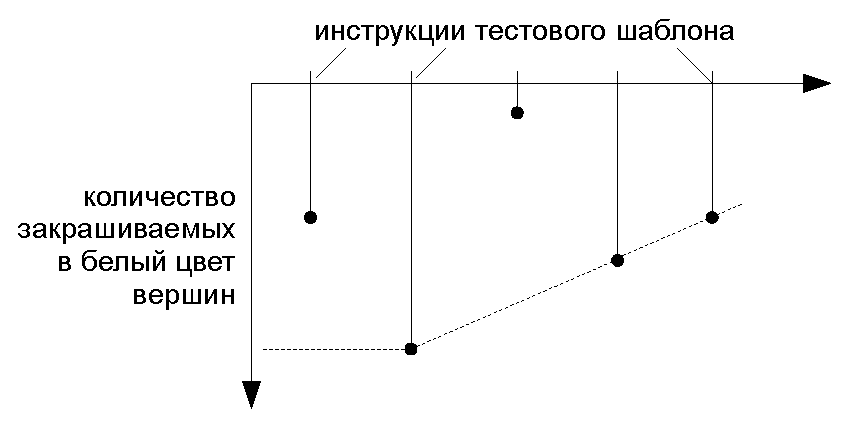
\includegraphics[width=0.6\textwidth]{2.theor/white_feeds}
  \caption{Последовательность закрашиваний белыми вершинами и ее выпуклая оболочка}\label{fig:white-feeds}
\end{figure}

На рисунке~\ref{fig:white-feeds} изображена последовательность из чисел-количеств вершин некоторой ветви, которые закрашивается в белый цвет очередной инструкцией тестового шаблона. Пунктиром обозначена ее <<выпуклая оболочка>>. Количество различных элементов в этой последовательности, которые входят в границу <<выпуклой оболочки>> соответствует количеству черных вершин в ветви. Вытеснение произойдет тогда, когда вся ветвь будет черной, т.е. когда количество различных инструкций, попадающих в границу <<выпуклой оболочки>>, превысит некоторую константную границу. Верно и обратное, вытеснение не произойдет, если количество этих инструкций будет меньше. Перекрашивание выполняется лишь на основе самой ветви. При обращении по тому ключу, который соответствует листу рассматриваемой ветви, количество черных вершин становится минимальным (равным 0). Итак, для стратегии вытеснения \PseudoLRU \emph{в качестве метрики вытеснения рассмотрим длину <<нижней>> черной части} пути к листу.

%Например, представленный на рисунке~\ref{fig:plru-useful} шаблон успевает покрасить 5 вершин ветви в черный цвет.
%
%\begin{figure}[t] \center
%  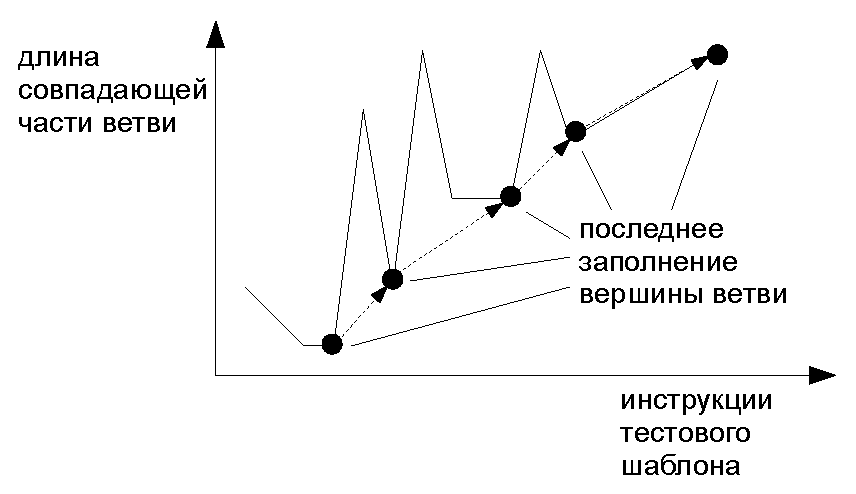
\includegraphics[width=0.6\textwidth]{2.theor/plru-useful}\\
%  \caption{Заполнение ветви черными вершинами в стратегии вытеснения
%  \PseudoLRU}\label{fig:plru-useful}
%\end{figure}

\begin{utv}
Инструкция $I$ считается полезной в случае стратегии вытеснения
\PseudoLRU, если все последующие инструкции затрагивают только те
вершины ветви, которые расположены выше вершины, перекрашиваемой инструкцией $I$ в черный цвет.
\end{utv}

Для вытеснения нужно не менее $\log_2 w$ полезных инструкций (длина ветви). Далее выражение $\log_2 w$ будет обозначаться буквой $W$.

Отличие этой метрики вытеснения от метрики вытеснения для \LRU
является \emph{немонотонность}. Это означает, что полезные
инструкции надо считать для каждого промаха заново ---
инструкции между двумя соседними промахами могут <<забелить>>
несколько вершин ветви, что уменьшит метрику вытеснения
(см.рис.~\ref{nonmonotonic}). Метрика для \LRU является монотонной,
потому что инструкции между промахами не могут уменьшить метрику
вытеснения -- либо не меняют, либо увеличивают ее, сдвигая
ключ к концу списка \LRU (см. рис.~\ref{monotonic}).
%Таким образом, ограничение, описывающее стратегию вытеснения
%\PseudoLRU, будет представлено дизъюнкцией ограничений по всем
%предыдущим кэш-промахам.

\begin{figure}[h] \center
  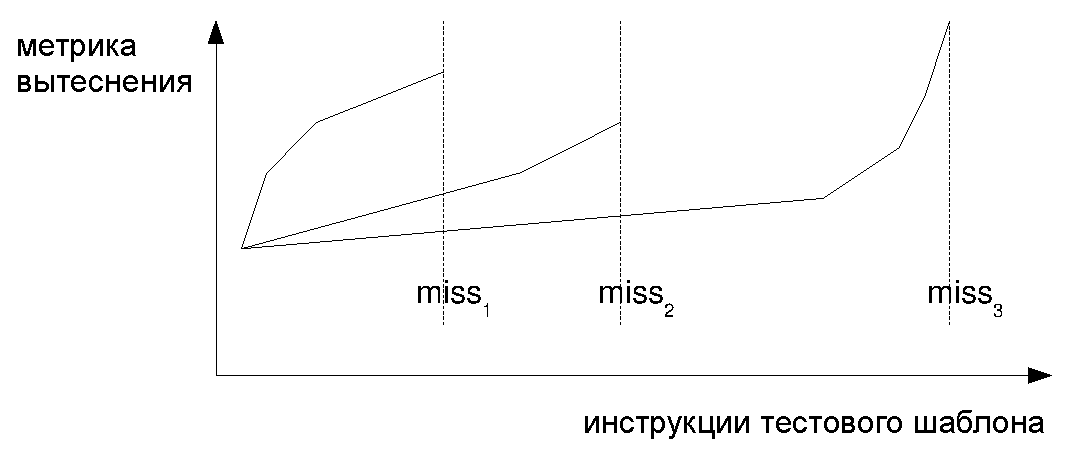
\includegraphics[width=0.6\textwidth]{2.theor/nonmonotonic}\\
  \caption{Немонотонная метрика вытеснения}\label{nonmonotonic}
\end{figure}

\begin{figure}[h] \center
  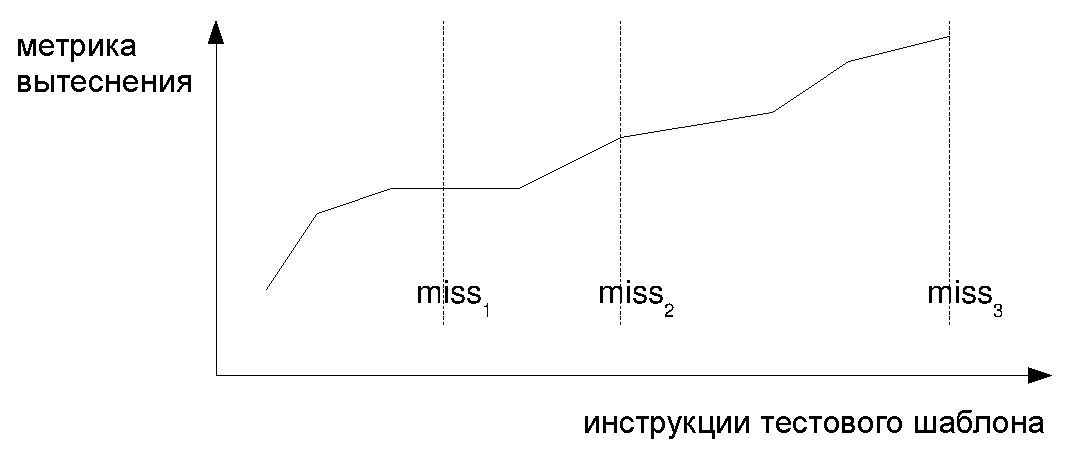
\includegraphics[width=0.6\textwidth]{2.theor/monotonic}\\
  \caption{Монотонная метрика вытеснения}\label{monotonic}
\end{figure}

Осталось записать понятие полезной инструкции для \PseudoLRU в виде
ограничений. Каждый ключ $k_i$ в регионе $R_i$ кроме своего значения
снабжен <<позицией>> $\pi_i$ ($\pi_i \in \{0..w{-}1\})$. Позиции -- это еще один набор переменных в добавление к ключам и регионам. Пусть надо записать ограничение, что ключ $k$ в регионе $R$ вытеснен в некоторой инструкции. Пусть $(k_1, R_1)$, $(k_2, R_2)$, ..., $(k_n, R_n)$ --- ключи и регионы предыдущих инструкций. Надо выяснить, когда заданная предыдущая инструкция будет полезной для вытеснения ключа $k$ из региона $R$. Инструкция не может быть полезной, пока не произошло в последний раз обращение к ключу $k$ в регионе $R$. В момент этого последнего обращения ветвь к нему становится целиком белой и начинается процесс вытеснения. Т.е. для дальнейших инструкций нам будет важно, каким позициям соответствуют в них ключи. Согласно определению полезные инструкции должны закрашивать больше белых вершин, чем закрашивают все последующие инструкции. И, наконец, эта логика в виде ограничений -- $(k_i, R_i, \pi_i)$ будет полезным для вытеснения ключа $k$ в регионе $R$, если выполнены все следующие условия:
\begin{itemize}
    \item $(k||R) \notin \{(k_i||R_i), (k_{i+1}||R_{i+1}), ..., (k_n||R_n)\}$ -- инструкция расположена после последнего обращения к $k$ в $R$;
    \item $R = R_i$ -- инструкция обращатеся в тот же регион;
    \item $P(\pi_i \oplus \pi,~\pi_{i+1} \oplus \pi) \wedge P(\pi_i \oplus \pi,~\pi_{i+2} \oplus \pi) \wedge ... \wedge P(\pi_i \oplus \pi,~\pi_{n-1} \oplus \pi)$ -- все последующие обращения должны пересекаться только в более верхних частях ветви (это выражает предикат $P$ для пары векторов); обращение в $n$'й инструкции должно быть промахом (потом это условие будет обеспечено); предикат $P(\delta_i, \delta_j)$ истинен тогда и только тогда, когда количество старших нулевых бит у $\delta_i$ больше количества старших нулевых бит у $\delta_j$, иными словами, только и только тогда, когда существует $k$ такое, что $\delta_i < 2^k \leqslant \delta_j$; с использованием битовых операций этот предикат можно записать в следующем виде: $P(\delta_i, \delta_j) \equiv (\delta_j > \delta_i~~\wedge~~\delta_j \oplus \delta_i > \delta_i)$, сравнения беззнаковые.
\end{itemize}

Итак, система уравнений для описания обращений по ключу $k$ в регион $R$ согласно методу функций полезности для \PseudoLRU:
\begin{itemize}
\item $k$ еще не вытеснен из региона $R$:
$$
\left\{\begin{array}{l}
(k||R) \in \{(t_1||r_1), ..., (t_m||r_m), (k_1||R_1), ..., (k_n||R_n)\}\\
\{(t_1||r_1), ..., (t_m||r_m)\} - \mbox{все разные}\\
\bigvee_{q:1..n:\mbox{miss}} \sum\limits_{i=1}^m u_{k,R}(t_i||r_i) + \sum\limits_{i=1}^q u_{k,R}(k_i||R_i) < w\\
\end{array} \right.
$$
\item $k$ вытеснен из региона $R$:
$$
\left\{\begin{array}{l} (k||R) \in \{(t_1||r_1), ..., (t_m||r_m), (k_1||R_1), ..., (k_n||R_n)\}\\
\{(t_1||r_1), ..., (t_m||r_m)\} - \mbox{все разные}\\
\bigwedge_{q:1..n:\mbox{miss}} \sum\limits_{i=1}^m u_{k,R}(t_i||r_i) + \sum\limits_{i=1}^q u_{k,R}(k_i||R_i) \geqslant w\\
\end{array} \right.
$$
\end{itemize}

$$u_{k,R} (s_i) \equiv \left\{\begin{array}{l}
(k||R) \notin \{(k_i||R_i), (k_{i+1}||R_{i+1}), ..., (k_n||R_n)\}\\
R = R(s_i)\\
P(\pi_i \oplus \pi,~\pi_{i+1} \oplus \pi)\\
P(\pi_i \oplus \pi,~\pi_{i+2} \oplus \pi)\\
... \\
P(\pi_i \oplus \pi,~\pi_{n-1} \oplus \pi)
\end{array}\right.
$$
$$s \equiv \langle (t_1,r_1), (t_2,r_2), ..., (t_m,r_m), (k_1, R_1), ..., (k_n,R_n) \rangle$$
$$R(s_i) \mbox{~--- вторая компонента~} s_i$$

Поскольку введены позиции, то надо еще в систему ограничений включить соотношение позиций и ключей --- конъюнкцию для каждой пары $(s_i,\pi_i)$ и $(s_j, \pi_j)$, где инструкция второй пары расположена после инструкции первой пары, ограничений:
\begin{itemize}
    \item если вторая инструкция --- попадание, то $$(\pi_i||R(s_i) = \pi_j||R(s_j)~\wedge$$ $$\pi_i||R(s_i) \notin \{\pi_{m_1}||R(s_{m_1}), \pi_{m_2}||R(s_{m_2}), \dots, \pi_{m_n}||R(s_{m_n})\}) \rightarrow s_i = s_j$$
    \item если вторая инструкция --- промах, то $$(\pi_i||R(s_i) = \pi_j||R(s_j)~\wedge$$ $$\pi_i||R(s_i) \notin \{\pi_{m_1}||R(s_{m_1}), \pi_{m_2}||R(s_{m_2}), \dots, \pi_{m_n}||R(s_{m_n})\}) \rightarrow s_i \neq s_j$$
\end{itemize}
где $(\pi_{m_1},R(s_{m_1})), (\pi_{m_2},R(s_{m_2})), \dots, (\pi_{m_n},R(s_{m_n}))$ --- позиции и регионы\\инструкций-промахов, расположенных между $i$'й и $j$'й инструкциями. В качестве $i$'й инструкции также надо рассмотреть и инициализирующие инструкции.

%Таблица~\ref{plru_table} содержит ограничения для разных случаев
%кэш-попаданий и кэш-промахов (см. утверждение~\ref{hit_miss_human}).
%В каждое из них включается ограничение на количество полезных
%инструкций согласно предлагаемой методике использования функций
%полезности. Полезности считаются относительно некоторого кэш-промаха
%(для их перебора используется сокращение $x_m : \mbox{miss}$).

Теорема, доказывающая корректность этих ограничений, приведена и доказана в приложении~\ref{proofs}.


\subsection{Разрешение уравнений, описывающих стратегии вытеснения}

Ограничения, которые предлагается генерировать для описания тестовых ситуаций, являются \emph{ограничениями мощности} (cardinality constraints). Это ограничения вида $C_1 \leqslant \sum_{i=1}^n a_i \leqslant C_2$, где $C_1, C_2$ -- неотрицательные целые числа, а $a_i$ принимают значения 0 или 1~\cite{smt_debugging, PiskacK08, KuncakR07,
Revesz05}. Речь идет об ограничении размера некоторого множества
элементов, заданного с помощью характеристической функции.
В~\cite{smt_debugging} проведено исследование способов записи
ограничений мощности и показано, что от формы записи зависит
эффективность разрешения этих ограничений. Например, ограничения
мощности можно рассматривать, как компактную форму записи уравнения
вида $\bigvee_{C_1 \leqslant C \leqslant C_2} \sum_{i=1}^n a_i = C$,
где равенство есть
\begin{itemize}
\item тождественная ложь, если $C < 0$ или $C > n$;
\item конъюнкция $\bigwedge_{1\leqslant i\leqslant n} (a_i = 0)$,
если $C = 0$;
\item дизъюнкция по всевозможным выборкам индексов $i_1, ..., i_C$, где
для каждого индекса $i_k$ справедливы свойства $1 \leqslant i_k
\leqslant n$ и $i_k < i_{k+1}$, конъюнкций $\bigwedge_{i_k} (a_{i_k}
= 1)$, если $1 \leqslant C \leqslant n$.
\end{itemize}

В данной работе не ставилась задача исследования способов разрешения ограничений мощности (с целью выбора наиболее эффективного способа их представления). Вместо этого были использованы
имеющиеся инструменты разрешения ограничений мощности~\cite{Z3, Yices}. Для записи оставшихся формул были использован язык битовых строк, для разрешения формул над которым существуют эффективные SMT-инструменты (например, Z3~\cite{Z3}).

%После устранения ограничений мощности в формуле остаются только
%ограничения на конечные множества тегсетов: принадлежности и
%непринадлежности тега конечному множеству тегсетов и равенства и
%неравенства битовых полей тегсетов. Поскольку конечные множества
%тегсетов известны (заданы перечислением тегсетов, которые в входят в
%это множество), то ограничения принадлежности и непринадлежности
%могут быть переписаны без использования этих отношений. Отношение
%принадлежности $x \in \{x_1, x_2, ..., x_n\}$ может быть переписано
%в виде дизъюнкции $(x = x_1) \vee (x = x_2) \vee ... \vee (x =
%x_n)$, а отношение непринадлежности $x \notin \{x_1, x_2, ...,
%x_n\}$ -- в виде конъюнкции $(x \neq x_1) \wedge (x \neq x_2) \wedge
%... \wedge (x \neq x_n)$.
%
%В результате получается предикат, в котором переменными величинами
%являются неотрицательные целые числа с конечной областью значений
%(тегсеты), над переменными возможны операции получения битового
%поля, в предикате используется отношение равенства и неравенства над
%битовыми полями. Кроме того, этот предикат задается с использованием
%ограничений мощности.
%
%Для разрешения такого рода предикатов можно было бы разрабатывать
%собственные процедуры распространения ограничений, но это свело бы
%на нет все усилия по выработке собственного представления стратегии
%вытеснения. Однако предлагаемые ограничения могут быть тривиальным
%образом выражены на языке теорий, для которых существуют эффективные
%разрешающие процедуры (битовые строки, неинтерпретируемые функции).
%Поэтому для записи и разрешения этих ограничений могут быть
%использованы SMT-инструменты~\cite{Z3}.

%%%%%%%%%%%%%%%%%%%%%%%%%%%%%%%%%%%%%%%%%%%%%%%%%%%%%%%%%%%%%%%%%%%
%
%\pagebreak
%\section{Ограничения, описывающие тестовые ситуации в некоторых
%частных случаях, для стратегии вытеснения \LRU}
%
%\subsection{Тестовые шаблоны без кэш-промахов}
%
%В случае тестовых шаблонов, в которых нет кэш-промахов, нет ни
%вытесняющих, ни вытесняемых тегсетов. Поэтому в таких шаблонов
%уравнения для кэш-попаданий имеют очень простой вид:
%
%$$
%\left\{
%\begin{array}{l}
%x \in D\\
%... (\mbox{тестовые ситуации на остальные буферы})\\
%\end{array}
%\right.
%$$
%
%\subsection{Тестовые шаблоны без кэш-попаданий}
%
%В случае тестовых шаблонов, в которых нет кэш-попаданий, надо
%генерировать ограничения для вытесняющих и лишь иногда для
%вытесняемых тегсетов. А именно, вытесняемый тегсет требуется лишь в
%том случае, когда кэш-промах вносит в кэширующий буфер ранее
%вытесненный тегсет. В этом случае для вытесняемого тегсета известен
%домен, что позволяет построить уравнения обозримого размера. Кроме
%того, поскольку отсутствуют кэш-попадания, повторные обращения к
%вытесняемым тегсетам (кроме кэш-промаха, который их может внести в
%кэширующий буфер) невозможны, что также упрощает генерируемые
%уравнения.
%
%В результате получается, что вытесняющий тегсет описывается в
%тестовом шаблоне без кэш-попаданий следующей системой уравнений:
%$$
%F'(x) \vee F''(x) \vee \bigvee_{\lambda_\delta \in D} F'''(x, \lambda_\delta)
%$$
%
%где
%
%$$F'(x) \equiv (x \notin D \wedge x \notin \{x_1, ..., x_n\})$$
%
%$$F''(x) \equiv (x \in \{x_1, ..., x_n\} \wedge \sum_{i=1}^n u''(x_i) \geqslant w)$$
%
%$$u''(x_i) \equiv (x\notin \{x_i, ..., x_n\} \wedge R(x_i) = R(x))$$
%
%$$F'''(x, \lambda_\delta) \equiv (x = \lambda_\delta \wedge x \notin
%\{x_1, ..., x_n\} \wedge \sum_{i=1}^n (R(x_i) = R(x)) \geqslant w -
%\delta + 1)$$
%
%\subsection{Короткие тестовые шаблоны}
%
%Будем называть тестовый шаблон \emph{коротким}, если в нем не более
%$w$ инструкций обращения к памяти. Очевидно, что любой короткий
%тестовый шаблон является простым. Из 7 случаев для коротких тестовых
%шаблонов остается всего 5 (первые два можно еще объединить в более
%компактную систему уравнений). В таблице~\ref{short_templates_table}
%предъявлены функции полезности и ограничения для коротких тестовых
%шаблонов в случае стратегии вытеснения \LRU. Соответствующая теорема
%корректности этих ограничений сформулирована и доказана в приложении~\ref{proofs}.
%
%\begin{table}[t]
%\begin{tabular}{|c|c|c|c|}
%\hline  & \centering случай &
%\begin{tabular}{c}переменная\\перебора\end{tabular} & система \\
%\hline \hline \multirow{-2}{*}{\rotatebox{90}{кэш-попадание}} &
%\makecell[c{p{0.3\textwidth}}]{тегсет находится в начальном
%состоянии буфера и он всё ещё не вытеснен} & $\lambda_\delta \in D$
%&
%$\left\{\begin{array}{l} x = \lambda_\delta\\
%\sum\limits^n_{i=1} u(x_i) \leqslant w - \delta
%\end{array}\right.$ \\ \hhline{~|---}
%& \makecell[c{p{0.3\textwidth}}]{тегсет уже встречался в шаблоне} &
%-- & $x \in \{x_1, ..., x_n\}$
%\\ \hline \hline \multirow{6}{*}{\rotatebox{90}{кэш-промах}}
%& \makecell[c{p{0.3\textwidth}}]{тегсет встречается впервые} & -- &
%$\left\{\begin{array}{l} x \notin D\\
%x \notin \{x_1, ..., x_n\}\\
%\end{array}\right.$\\ \hhline{~|---} &
%\makecell[c{p{0.3\textwidth}}]{тегсет находился в начальном
%состоянии буфера и был вытеснен} & $\begin{array}{c}\lambda_\delta
%\in D,\\\delta \geqslant w-n+1\end{array}$ &
%$\left\{\begin{array}{l} x = \lambda_\delta\\
%x \notin \{x_1, ..., x_n\}\\
%\sum\limits^n_{i=1} u(x_i) > w - \delta\\
%\end{array}\right.
%$ \\ \hline
%\end{tabular}
%
%%где функция полезности определена следующим образом:
%$$u(x_i) \equiv
%\left\{\begin{array}{l} x_i \in \{ \lambda_{\delta+1}, ...,
%\lambda_w\}~\wedge~x_i \notin \{x_1, ..., x_{i-1}\}, \mbox{если}~S_i
%= \mbox{hit}\\
%R(x_i) = R(x), \mbox{если}~S_i = \mbox{miss}
%\end{array}\right.
%$$
%\caption{Таблица систем уравнений для тестовых ситуаций в кэширующих
%буферах для коротких тестовых шаблонов в случае стратегии вытеснения
%\LRU}\label{short_templates_table}
%\end{table}
%
%
%
%%\begin{landscape}
%%\begin{table}
%%\begin{tabular}{|c|c|c|c|c|c|}
%%\hline  & \centering случай &
%%\begin{tabular}{c}переменная\\перебора\end{tabular} & система &
%%\begin{tabular}{c}функция\\полезности\\для кэш-\\попадания\end{tabular} &
%%\begin{tabular}{c}функция\\полезности\\для кэш-\\промаха\end{tabular} \\
%%\hline \hline \multirow{-2}{*}{\rotatebox{90}{кэш-попадание}} &
%%\makecell[c{p{0.3\textwidth}}]{тегсет находится в начальном
%%состоянии буфера и он всё ещё не вытеснен} & $\lambda_\delta \in
%%D$ &
%%$\left\{\begin{array}{l} x = \lambda_\delta\\
%%\sum\limits^n_{i=1} u(x_i) \leqslant w - \delta
%%\end{array}\right.
%%$ &
%%\begin{tabular}{c}
%%$x_i \in \{ \lambda_{\delta+1}, ..., \lambda_w\}$\\
%%$\wedge~x_i \notin \{x_1, ..., x_{i-1}\}$
%%\end{tabular}
%%& $R(x_i) = R(x)$
%%\\ \hhline{~|-----}
%%& \makecell[c{p{0.3\textwidth}}]{тегсет уже встречался в шаблоне} &
%%-- & $x \in \{x_1, ..., x_n\}$ & -- & --
%%\\ \hline \hline \multirow{6}{*}{\rotatebox{90}{кэш-промах}}
%%& \makecell[c{p{0.3\textwidth}}]{тегсет встречается впервые} & -- &
%%$\left\{\begin{array}{l} x \notin D\\
%%x \notin \{x_1, ..., x_n\}\\
%%\end{array}\right.
%%$ & -- & -- \\ \hhline{~|-----} &
%%\makecell[c{p{0.3\textwidth}}]{тегсет находился в начальном
%%состоянии буфера и был вытеснен} &
%%$\begin{array}{c}\lambda_\delta \in D,\\\delta \geqslant
%%w-n+1\end{array}$ &
%%$\left\{\begin{array}{l} x = \lambda_\delta\\
%%x \notin \{x_1, ..., x_n\}\\
%%\sum\limits^n_{i=1} u(x_i) > w - \delta\\
%%\end{array}\right.
%%$ &
%%\begin{tabular}{c}
%%$x_i \in\{\lambda_{\delta+1}, ..., \lambda_w\}$\\
%%$\wedge~x \notin \{x_1, ..., x_{i-1}\}$\\
%%\end{tabular}
%%&
%%\begin{tabular}{c}
%%$R(x_i) = R(x)$\\
%%\end{tabular}
%%\\ \hline
%%\end{tabular}
%%\caption{Таблица систем уравнений для тестовых ситуаций в кэширующем буфере
%%для коротких тестовых шаблонов в случае стратегии вытеснения
%%\LRU}\label{short_templates_table}
%%\end{table}
%%\end{landscape}
%
%
%\subsection{Генерация тестовых данных для кэш-памяти, содержащей
%<<грязные>> ячейки}
%
%Любая ячейка в кэш-памяти может быть помечена \emph{грязной}
%(\emph{invalid}). Это означает, что данные, находящиеся в кэширующем
%буфере по этому адресу, не могут использоваться в качестве данных,
%хранящихся в памяти по этому адресу.
%
%Рассмотренные ранее в этой работе случаи не учитывали грязные ячейки
%кэширующем буфере, хотя они зачастую присутствуют в микропроцессоре
%после его запуска -- с таким состоянием кэширующего буфера работают
%первые после запуска микропроцессора инструкции.
%
%Кэш-попадание возникает в том случае, когда требуемые данные
%присутствуют среди <<чистых>> ячеек кэширующего буфера. Кэш-промах
%возникает в том случае, когда требуемых данных нет среди <<чистых>>
%ячеек. Причем при наличии <<грязных>> ячеек вытеснения может и не
%произойти. А именно, если все ячейки набора, с которым работает
%инструкция, являются <<чистыми>>, то происходит вытеснение согласно
%стратегии вытеснения, остальные наборы не меняются. Если же среди
%ячеек набор есть <<грязные>> ячейки, то вытеснение не происходит, а
%на место одной из <<грязных>> ячеек помещаются данные из основной
%памяти по заданному адресу и ячейка объявляется <<чистой>>.
%Остальные ячейки не меняются. В стратегии вытеснения \LRU эта бывшая
%<<грязная>> ячейка становится самой новой.
%
%Для генерации тестовых данных для кэширующих буферов с грязными
%ячейками предлагается применять ограничения с функциями полезности.
%Примечательно, что наличие грязных ячеек не меняет качественно
%систему уравнений.
%
%В данном разделе рассматривается случай, когда начальное состояние
%микропроцессора известно. Кроме того, рассматриваемый случай
%учитывает отсутствие инструкций в тестовом шаблоне, которые
%превращали бы <<чистые>> ячейки в <<грязные>> (т.е. все такие
%изменения должны делаться явно вне тестовых шаблонов).
%
%\subsubsection{случай полностью-ассоциативного кэширующего буфера}
%
%В случае полностью-ассоциативных кэширующих буферов очевидно, что
%первые кэш-промахи будут заполнять <<грязные>> ячейки. Пусть $N$ --
%количество <<грязных>> ячеек в начальном состоянии кэширующего
%буфера, а $L_0$ -- начальное состояние (выражение) кэширующего
%буфера (только <<чистые>> ячейки). Тогда для тестовых ситуаций надо
%генерировать такие ограничения ($L$ -- выражение для состояния
%кэширующего буфера перед исполнением инструкции, $L'$ -- выражение
%для состояния кэширующего буфера после исполнения инструкции):
%\begin{itemize}
%\item для \emph{кэш-попадания} hit($x$) генерируются ограничения
%$$
%\left\{
%\begin{array}{l}
%x \in L\\
%L' \equiv L\\
%\end{array}
%\right.
%$$
%
%\item для \emph{кэш-промаха} miss($x$), если это один из первых $N$
%кэш-промахов, генерируются ограничения:
%$$
%\left\{
%\begin{array}{l}
%x \notin L\\
%L' \equiv L \cup \{x\}\\
%\end{array}
%\right.
%$$
%
%\item для \emph{кэш-промаха} miss($x$), являющегося по счету более
%чем $N$'м кэш-промахом тестового шаблона, генерируются ограничения:
%$$
%\left\{
%\begin{array}{l}
%x \notin L\\
%x' \in L\\
%L' \equiv L\setminus\{x'\} \cup \{x\}\\
%displaced(x', L)\\
%\end{array}
%\right.
%$$
%\end{itemize}
%
%Предикат $displaced(x', L)$ истинен, если $x'$ является вытесняемым
%тегом в текущем состоянии кэширующего буфера $L$. Для стратегии
%вытеснения \LRU этот предикат может быть записан с использованием
%тех же диапазонов вытеснения, что и для кэширующего буфера без
%<<грязных>> ячеек (см.п.~\ref{LRU_constraints}). А именно, диапазон
%вытеснения начинается на инструкции, которая последний раз перед
%вытеснением тега обращается к нему. Тогда между этой инструкцией и
%инструкцией, вытесняющей $x$, должны быть обращения ко всем
%остальным тегам текущего состояния кэширующего буфера. Эта логика
%может быть записана в виде тех же уравнений, что и в
%пункте~\ref{LRU_constraints}. Нетрудно проверить, что для
%кэширующего буфера с <<грязными>> ячейками остается справедливой
%лемма о невложенных диапазонах вытеснения, что доказывает
%корректность использования ограничений из
%пункта~\ref{LRU_constraints} для кэширующего буфера с <<грязными>>
%ячейками.
%
%\subsubsection{случай наборно-ассоциативного кэширующего буфера}
%
%В этом пункте будет показано, что ограничения для кэширующего
%буфера, начальное состояние которого содержит <<грязные>> ячейки,
%качественно не отличаются от ограничений для кэширующего буфера без
%<<грязных>> ячеек.
%
%Аналогично тому, как это делалось для кэширующих буферов без
%<<грязных>> ячеек, для тестовых ситуаций на кэширующие буферы с
%<<грязными>> ячейками тоже возможно следующее исчерпывающее
%выделение случаев:
%\begin{itemize}
%\item кэш-попадание тега:
%    \begin{enumerate}
%    \item данный тег находился в начальном состоянии кэширующего буфера и не был
%    вытеснен к моменту данной инструкции;
%    \item данный тег был внесен в кэширующий буфер одной из инструкций
%    кэш-промаха и с тех пор не был вытеснен;
%    \end{enumerate}
%\item кэш-промах тега:
%    \begin{enumerate}
%    \item данный тег не встречался ранее (не находился в начальном
%    состоянии кэширующего буфера и не был внесен какими-либо кэш-промахами);
%    \item данный тег был ранее вытеснен из кэширующего буфера и с тех пор
%    не был внесен в кэширующий буфер вновь.
%    \end{enumerate}
%\end{itemize}
%
%Соответствующие ограничения приведены в
%таблице~\ref{dirty_hit_miss_table}.
%
%
%В таблице~\ref{dirty_hit_miss_table} символ $\Delta$ означает
%количество <<чистых>> ячеек в начальном состоянии того региона, про
%который идет речь в уравнении. На самом деле $\Delta$ есть функция
%региона ($\Delta = \Delta(\lambda_\delta)$), но для сокращения
%записи оставлен только функциональный символ. Кроме того, в
%приведенных уравнениях домен переменной включает только <<чистые>>
%ячейки.
%
%Сходства уравнений (со случаем кэширующих буферов без <<грязных>>
%ячеек) удалось добиться за счет рассмотрения <<грязных>> ячеек, как
%ячеек с наименьшим счетчиком \LRU, которые не участвуют в
%определении нахождения тега в кэширующих буферах. Поэтому в функциях
%полезности участвуют множества не $\{\lambda_{\delta+1}, ...,
%\lambda_w\}$, а множества $\{\lambda_{\delta+1}, ...,
%\lambda_\Delta\}$. Все <<чистые>> ячейки получили первые индексы,
%т.е. индексы всех от 1 до $\Delta$.
%
%%\begin{theorem}[корректность использования функций полезности для
%%записи \LRU в случае наличия <<грязных>> ячеек в начальном состоянии
%%кэширующего буфера] Тестовая программа, построенная по ограничениям,
%%которые сгенерированы с использованием предъявленных в
%%таблице~\ref{dirty_hit_miss_table} функций полезности, в случае
%%наличия <<грязных>> ячеек в начальном состоянии кэширующего буфера
%%удовлетворяет своему тестовому шаблону.
%%\end{theorem}
%%\begin{proof}
%%  //TODO
%%\end{proof}
%
%Для приведенных ограничений также могут быть применены эвристики,
%сокращающие их количество, которые были упомянуты для кэширующих
%буферов без <<грязных>> ячеек. Кроме того, в данном случае возможна
%дополнительная эвристика \emph{ограничение на $\delta$}: если
%$\delta + 1 < \Delta$, то функция полезности, в которую входит
%множество $\{\lambda_{\delta+1}, ..., \lambda_\Delta\}$, равна 0.
%
%%\subsection{Функции полезности для зеркальной генерации тестовых
%%данных}
%%
%%Рассмотрим ограничения, генерируемые для тестовых шаблонов
%%зеркальным методом с использованием функций полезности. По сравнению
%%с представленными ограничениями (см. табл.~\ref{hit_miss_table})
%%зеркальная генерация имеет свои особенности:
%%\begin{enumerate}
%%  \item множества констант (как, например, $L, D$) не используются,
%%  поэтому в ограничениях будут отсутствовать соответствующие им
%%  случаи;
%%  \item так как теги инструкций тестового шаблона должны появиться
%%  среди инициализирующей последовательности, то для вытеснения
%%  требуется $w-1$ инструкций, где $w$ -- ассоциативность кэширующего буфера;
%%  \item учет полезных инструкций начинается уже в инициализирующей
%%  последовательности, тем самым необходимо сформулировать функцию
%%  полезности для инициализирующих инструкций.
%%\end{enumerate}
%%
%%Следующая теорема описывает функцию полезности для инициализирующих
%%инструкций и описывает ограничения, генерируемые для тестовых
%%шаблонов зеркальным методом с использованием функций полезности
%%(количество инициализирующих инструкций зафиксировано, оно будет
%%обозначено параметром $m$):
%%
%%\begin{theorem}[Корректность ограничений, генерируемые зеркальным методом с
%%использованием функций полезности для
%%\LRU]\label{correct_mirror_LRU} Пусть $t_1, t_2, ..., t_m$ -- теги
%%инициализирующей последовательности, $x$ -- текущий тег тестового
%%шаблона, $x_1, x_2, ..., x_n$ -- теги предыдущих инструкций
%%тестового шаблона, причем $x \in \{t_1, ..., t_m, x_1, ..., x_n\}$ и
%%$\{t_1, ..., t_m\}$ --- все разные. Тогда $x$ не вытеснен согласно
%%определению на списках тогда и только тогда, когда
%%$$\sum\limits_{i=1}^{m+n} u_x(s_i) < w$$
%%где последовательность $s \equiv \langle t_1, ..., t_m, x_1, ...,
%%x_n\rangle$, а функция полезности определена следующим образом:
%%$$u_x(s_i) \equiv (x \notin \{s_i, ..., s_{m+n}\} \wedge
%%R(x) = R(s_i) \wedge s_i \notin\{s_{i+1},..., s_{m+n}\})$$
%%
%%%$$\sum\limits_{i=1}^m \tilde{u}_x(t_i) + \sum\limits_{i=1}^n u_x(x_i) < w$$
%%%где функции полезности определены следующим образом:
%%%$$\begin{array}{c}
%%%\tilde{u}_x(t_i) \equiv (x \notin \{t_i, ..., t_m, x_1, ..., x_n\}
%%%\wedge R(x) = R(t_i))\\u_x(x_i) \equiv (x \notin \{x_i, ..., x_n\}
%%%\wedge R(x) = R(x_i))\end{array}$$
%%
%%%$$\begin{array}{c}u_x(x_i) \equiv (x \notin \{x_i, ..., x_n\} \wedge R(x) =
%%%R(x_i)), \mbox{если}~S_i=\mbox{miss}\end{array}$$
%%%$$\begin{array}{c}u_x(x_i) \equiv (x \notin \{x_i, ..., x_n\} \wedge R(x) =
%%%R(x_i) \wedge \sum\limits_{j=1}^{m} \tilde{c}_{x_i}(t_j) = 0
%%%\wedge \sum\limits_{j=1}^{i-1} c_i(x_j) = 0),\\
%%%\mbox{если}~S_i=\mbox{hit}\end{array}$$
%%%$$c_i(x_j) \equiv (x \notin \{x_j, ..., x_{i-1}\} \wedge x_i = x_j)$$
%%%$$\tilde{c}_{x_i}(t_j) \equiv (x \notin \{t_j, ..., t_m, x_1, ..., x_{i-1}\} \wedge x_i = t_j)$$
%%\end{theorem}
%%\begin{proof}
%%//TODO написать правильное доказательство
%%
%%сумма полезных - это количество различных тегов, тогда полезными будем считать инструкции тестового шаблона, которые обращаются к разным тегам, при этом ко всем различным тегам есть инструкция; различные - например, последние; отсюда и функция полезности.
%%
%%%Воспользуемся леммой~\ref{hit_II}. При этом в качестве
%%%последовательности тегов тестового шаблона в этой лемме рассмотрим
%%%последовательность $t_1, t_2,~\dots,~t_m,~x_1,~x_2,~\dots,~x_n$.
%%%Согласно лемме тестовая ситуация на $x$ выполнена при
%%%соответствующем условии на сумму функций полезности от элементов
%%%этой последовательности. Функции полезности для
%%%$x_1,~x_2,~\dots,~x_n$ без изменений переходят из формулировки
%%%леммы~\ref{hit_II} в данную теорему. Функцию полезности для $t_1,
%%%t_2,~\dots,~t_m$ из формулировки леммы~\ref{hit_II} получить нельзя,
%%%поскольку неизвестна тестовая ситуация на эти теги. Однако, вспомнив
%%%определение полезной инструкции, функцию полезности для этих тегов
%%%получить несложно. А именно, тег $t_i$ будет полезным, если он
%%%продвигает $x$ к концу списка \LRU после последнего обращения к $x$.
%%%Если после последнего обращения к $x$ сам тег $t_i$ встречается
%%%впервые, то он будет полезным (см. доказательство
%%%леммы~\ref{hit_II}). Если же после последнего обращения к $x$ $t_i$
%%%встречается не в первый раз, то он не двигает $x$ к концу списка,
%%%что, тем самым, означает бесполезность $t_i$. Но поскольку все $t_i$
%%%разные, то повторное обращение возможно лишь среди
%%%$x_1,~x_2,~\dots,~x_n$ -- поэтому в функцию полезности для этих
%%%тегов добавлено отличие от $t_1,~t_2,~\dots,~t_m$.
%%\end{proof}
%%%\begin{sld}[Корректность ограничений, генерируемые зеркальным методом с
%%%использованием функций полезности для полностью ассоциативного \LRU
%%%буфера] Пусть $t_1, t_2, ..., t_m$ -- теги инициализирующей
%%%последовательности, $x$ -- текущий тег тестового шаблона, $x_1, x_2,
%%%..., x_n$ -- теги предыдущих инструкций тестового шаблона, причем $x
%%%\in \{t_1, ..., t_m, x_1, ..., x_n\}$ и $\{t_1, ..., t_m\}$ --- все
%%%разные. Тогда $x$ не вытеснен из полностью ассоциативного буфера
%%%согласно определению на списках тогда и только тогда, когда
%%%$$x \in \{s_{m+n-w+1}, ..., s_{m+n}\}$$ где последовательность $s
%%%\equiv \langle t_1, ..., t_m, x_1, ..., x_n\rangle$.
%%%\end{sld}
%%%\begin{proof}
%%%  //TODO
%%%\end{proof}
%%
%%Из теоремы~\ref{correct_mirror_LRU} следует система уравнений для
%%описания тестовой ситуации $S$ тега $x$, генерируемая зеркальным
%%методом с использованием функций полезности для \LRU (функции
%%полезности приведены в формулировке
%%теоремы~\ref{correct_mirror_LRU}):
%%\begin{itemize}
%%\item если $S$ = hit, то
%%$$
%%\left\{\begin{array}{l} x \in \{t_1, ..., t_m, x_1, ..., x_n\}\\
%%\sum\limits_{i=1}^m u_x(t_i) + \sum\limits_{i=1}^n u_x(x_i) < w\\
%%\{t_1, ..., t_m\} - \mbox{все разные}\\
%%\end{array} \right.
%%$$
%%\item если $S$ = miss, то
%%$$
%%\left\{\begin{array}{l} x \in \{t_1, ..., t_m, x_1, ..., x_n\}\\
%%\sum\limits_{i=1}^m u_x(t_i) + \sum\limits_{i=1}^n u_x(x_i)
%%\geqslant w\\
%%\{t_1, ..., t_m\} - \mbox{все разные}\\
%%\end{array} \right.
%%$$
%%\end{itemize}
%%
%%%Стоит заметить, что функции полезности добавили новое дополнительное
%%%условие на теги инициализирующих инструкций: они должны быть
%%%различными. В этом выражается свойство <<простоты>> инициализирующей
%%%последовательности, эта последовательность не должна содержать
%%%сложной внутренней последовательности изменений состояния
%%%кэширующего буфера.

\chapter{Апробация}

В этой главе показывается, что предлагаемых в диссертации средств
описания модели состояния MMU и инструкций достаточно для генерации
тестов таких трех часто используемых архитектур как MIPS~\cite{mips64_II},
PowerPC~\cite{??????????????} и Pentium~\cite{???????????????}. При
рассмотрении архитектур важными будут следующие вопросы:
\begin{enumerate}
    \item описываются ли инструкции в виде ограничений на битовые
    строки в документации?
    \item описывается ли модель состояния MMU в виде лишь таблиц? нет ли там чего-нибудь, не сводящегося к таблице?
    \item хватает ли предлагаемых средств для описания трансляции адреса ?
\end{enumerate}

В разделе ??????????? описаны эксперименты по оценке длины шаблонов, для
которых можно эффективно строить тесты предлагаемыми в диссертации
методами (и оценка переиспользования и пр????????). Заканчивается глава
сравнением особенностей предлагаемого метода генерации тестов по
тестовым шаблонам с методом, предлагаемым инструментом
Genesys-Pro~\cite{????????????????}.

%% отвечаем на следующие вопросы:
% 1. описываются ли инструкции в виде ограничений на битовые строки в документации
% 2. описывается ли модель состояния MMU в виде лишь таблиц? нет ли там чего-нибудь, не сводящегося к таблице?
% -> структура TLB
% 3. хватает ли средств для описания трансляции адреса ?
% -> поток данных, описывающих трансляцию
% режимы работы (real mode, protected mode)

% таблица - то, что представляется множеством строк,
% строка представляется набором полей ключа и полей данных

%% схема описания компонента MMU:
% 1. поля строк
% 2. количество строк
% 3. битовая длина номера региона (тип таблицы - полностью-ассоциативная, ....)
% 4. стратегия вытеснения
% 5. предикат keyMatch
% 6. особенности компонента (чего-то более одного, чего-то быть не может, ...) - например, одна строка хранит несколько подряд данных

% в MIPS R12000 появилась кэш-память адресов переходов (32 строки), но она не относится к MMU данных

\section{Генерация тестов для архитектуры MIPS}

%\begin{utv}
%Для архитектуры MIPS возможно применение применение методов, описыванных в диссертации, для генерации тестовых программ по тестовым шаблонам; причем методов достаточно
%для полного описания поведения MMU микропроцессоров архитектуры MIPS.
%\end{utv}

Документация по архитектуре MIPS представлена ................~\cite{??????????}. Документ
.... содержит описания инструкций, которые действительно описываются в виде набора
операций над битовыми строками.

<пример страницы документации>

Документ ...... содержит описание подсистемы управления памяти в микропроцессорах
MIPS. Для работы с данными она содержит следующие блоки (количественные
характеристики приведены для микропроцессора MIPS R10000~\cite{R10000}):
\begin{itemize}
  \item \emph{кэш-память данных первого уровня (D-Cache-1)}:
        \begin{itemize}
            \item размер: 32 кБ;
            \item поля строк: тэг физического адреса (ключ), данные (данные);
            \item битовая длина номера региона: 6 (наборно-ассоциативная кэш-память);
            \item количество строк в регионе: 2;
            \item стратегия вытеснения \LRU;
        \end{itemize}
  \item \emph{кэш-память второго уровня (Cache-2)}:
        \begin{itemize}
            \item размер: от 512 кБ до 16 МБ;
            \item поля строк: тэг физического адреса для кэш-памяти второго уровня (ключ), данные (данные) (16 или 32 слова);
            \item количество строк в регионе: 2;
            \item стратегия вытеснения \LRU;
        \end{itemize}
         Cache-2 является внешней;
  \item \emph{TLB (Joint-TLB)}:
        \begin{itemize}
            \item поля строк: r, vpn/2, g, asid (ключи), pfn0, cca0, v0, c0, d0, pfn1, cca1, v1, c1, d1 (данные);
            \item битовая длина номера региона: 0 (полностью-ассоциативный TLB);
            \item количество строк в регионе: 64;
            \item вытеснение программное (т.е. стратегия вытеснения none);
            \item размер виртуального адреса: 44 бита;
            \item размер физического адреса: 40 бит;
        \end{itemize}
        одна строка TLB хранит информацию про две соседние страницы виртуальной
        памяти;
  \item \emph{буфер TLB (D-TLB)}:
        \begin{itemize}
            \item поля строк те же, что и для Joint-TLB;
            \item битовая длина номера региона: 0 (полностью-ассоциативный);
            \item количество строк в регионе: 8;
            \item стратегия вытеснения \LRU;
        \end{itemize}
\end{itemize}

Другие блоки для обращения в память не используются.

Осталось показать, что трансляция адреса также может быть представлена в виде
отношений на битовых строках и обращениях в таблицы. Обычное выполнение обращения к памяти в MIPS следующее:
\begin{enumerate}
    \item на основе аргументов инструкции формируется \emph{виртуальный адрес};
    \item заменой номера страницы виртуальной памяти на номер фрейма физической памяти формируется \emph{физический адрес};
    \item по физическому адресу, если нужно, осуществляется обращение в кэш-память иди, если данных по физическому адресу нет в кэш-памяти, обращение в оперативную память.
\end{enumerate}

В зависимости от значения виртуального адреса и состояния управляющих регистров возможны следующие варианты трансляции адреса:
\begin{itemize}
  \item для виртуального адреса трансляция проходит через TLB (см.рис.~\ref{fig:mips_address_translation});
  \item для виртуального адреса трансляция проходит без таблиц (физический адрес --- битовая строка --- является результатом битовых операций над виртуальным адресом --- битовой строкой).
\end{itemize}

\begin{figure}[h] \center
  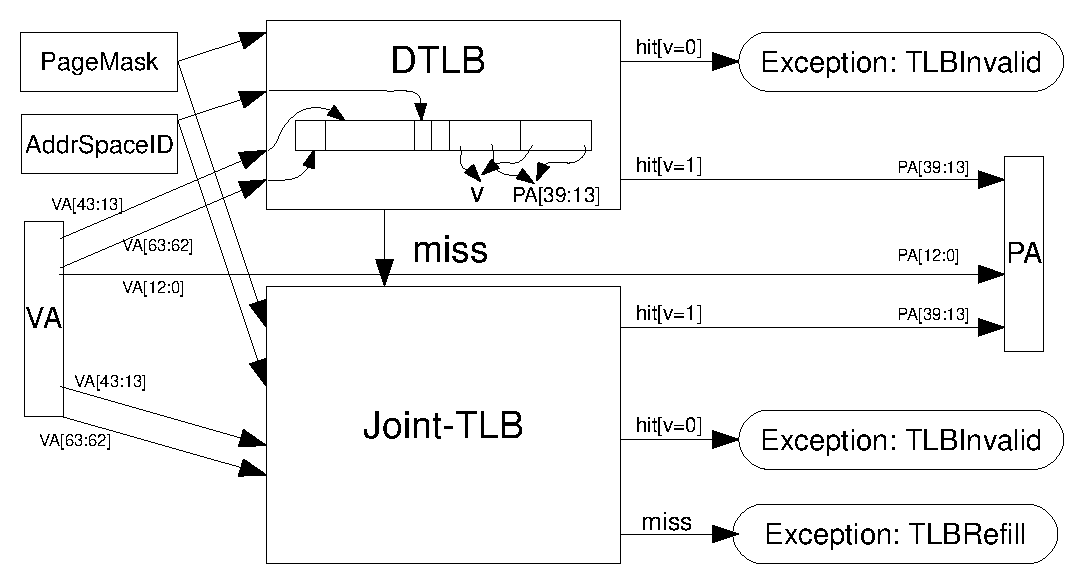
\includegraphics[width=0.8\textwidth]{4.analysis/mips_addrtrans}\\
  \caption{Трансляция адреса в MIPS}\label{fig:mips_address_translation}
\end{figure}

\section{Генерация тестов для архитектуры PowerPC}

Документация по архитектуре PowerPC представлена ................~\cite{??????????}. Документ
.... содержит описания инструкций, которые действительно описываются в виде набора
операций над битовыми строками.

<пример страницы документации>

Документ ...PowerPC Operating Environment Architecture (Book III, Version 2.01)... содержит описание подсистемы управления памяти в микропроцессорах PowerPC. Для работы с данными она содержит следующие блоки (количественные
характеристики приведены для микропроцессора PowerPC 970FX
~\cite{PowerPC970FXUserManual}% -- см. рис.~\ref{powerpc_mmu_scheme}
):
\begin{itemize}
  \item \emph{кэш-память данных первого уровня (D-Cache-1)}:
        \begin{itemize}
            \item размер: 32 кБ;
            \item поля строк: тэг физического адреса (ключ), данные (данные);
            \item битовая длина номера региона: 7 (наборно-ассоциативная кэш-память);
            \item количество строк в регионе: 2;
            \item стратегия вытеснения \LRU;
        \end{itemize}
  \item \emph{кэш-память второго уровня (Cache-2)}:
        \begin{itemize}
            \item размер: 512 кБ;
            \item поля строк: тэг физического адреса (ключ), данные (данные);
            \item битовая длина номера региона: 11 (наборно-ассоциативная кэш-память);
            \item количество строк в регионе: 8;
            \item стратегия вытеснения \LRU;
        \end{itemize}
  \item \emph{таблица страниц виртуальной памяти (PageTable)}:
        \begin{itemize}
            \item поля строк: номер страницы виртуальной памяти (ключ), номер фрейма физической памяти (данные);
            \item битовая длина номера региона: 65;
            \item количество строк в регионе: 1;
            \item вытеснение программное;
            \item размер эффективного адреса: 64 бита;
            \item размер виртуального адреса: 65 бит;
            \item размер физического адреса: 42 бита;
        \end{itemize}
        на самом деле таблица страниц виртуальной памяти организована в виде хэш-таблицы, но для тестирования этот момент не важен --- главное, что это соответствие номеров страниц виртуальной памяти номерам фреймов физической памяти, причем необязательно представлены все страницы виртуальной памяти;
  \item \emph{D-TLB} (кэш таблицы страниц):
        \begin{itemize}
            \item поля строк: номер страницы виртуальной памяти (ключ), номер фрейма физической памяти (данные);
            \item битовая длина номера региона: 8 (наборно-ассоциативный);
            \item количество строк в регионе: 4;
            \item стратегия вытеснения \LRU;
        \end{itemize}
  \item \emph{сегментные регистры (SLB, Segment Lookaside Buffer)}:
        \begin{itemize}
            \item поля строк: effective segment id (ключ), virtual segment id (данные), биты U/S, X, V (данные);
            \item битовая длина номера региона: 0 (полностью ассоциативный);
            \item количество строк в регионе: 64;
            \item вытеснение программное;
        \end{itemize}
        используются для получения виртуального адреса по эффективному;
  \item \emph{буфер непосредственной трансляции адресов (D-ERAT)}:
        \begin{itemize}
            \item поля строк: номер <<эффективной страницы>> (ключ), номер фрейма физической памяти (данные), биты (данные);
            \item битовая длина номера региона: 6 (наборно-ассоциативная таблица);
            \item количество строк в регионе: 2;
            \item стратегия вытеснения \FIFO;
        \end{itemize}
\end{itemize}

Другие блоки для обращения в память не используются.

Осталось показать, что трансляция адреса также может быть представлена в виде
отношений на битовых строках и обращениях в таблицы. Обычное выполнение обращения к памяти в PowerPC следующее:
\begin{enumerate}
    \item аргументы инструкции обращения к памяти формируется \emph{эффективный адрес};
    \item заменой номера сегмента из эффективного адреса получается \emph{виртуальный адрес};
    \item заменой номера виртуальной страницы в виртуальном адресе на номер фрейма физической памяти получается \emph{физический адрес};
    \item по физическому адресу, если нужно, осуществляется обращение в кэш-память иди, если данных по физическому адресу нет в кэш-памяти, обращение в оперативную память.
\end{enumerate}
 
В зависимости от состояния управляющих регистров возможны следующие варианты трансляции адреса:
\begin{itemize}
  \item <<трансляция выключена>>; физический адрес вычисляется по эффективному без обращения к каким-либо таблицам; (а как же ERAT ????)
  \item .........................
\end{itemize}

%\section{Генерация ограничений для архитектуры Alpha}
%
%\begin{utv}
%Для архитектуры Alpha возможно применение применение методов
%генерации ограничений, описыванных в диссертации, для генерации
%тестовых программ по тестовым шаблонам.
%\end{utv}
%
%Рассмотрим исполнение инструкции обращения к памяти в
%микропроцессоре архитектуры Alpha. MMU в микропроцессорах Alpha
%включает в себя  (количественные характеристики приведены для
%микропроцессора Alpha 21264~\cite{HennessyPatterson3rd} -- см.
%рис.~\ref{alpha_mmu_scheme}):
%\begin{itemize}
%  \item \emph{кэш-память данных первого уровня (D-Cache-1)}:
%  virtually indexed physically tagged, размер 64 килобайта,
%  наборно-ассоциативный, количество секций равно 2, стратегия вытеснения
%  \LRU, размер строки кэш-памяти 64 байта;
%  \item \emph{кэш-память второго уровня (Cache-2)}: physically
%  indexed physically tagged, прямого отображения, размер от 1 до 16
%  мегабайт
%  \item \emph{таблица TLB (D-TLB)}: 128 строк, полностью
%  ассоциативная, размер виртуального адреса 48/43 бит, размер физического адреса
%  44/41 бит, размер страницы виртуальной памяти от 8 килобайт до 4
%  мегабайт;
%  \item \emph{буфер вытесненных данных (VictimBuffer)}: полностью
%  ассоциативный, количество строк равно 8, стратегия
%  вытеснения \FIFO.
%\end{itemize}
%Таким образом, основная проблема при записи ограничений -- большой
%размер содержимого кэш-памяти.
%
%Инструкция может содержать тестовые ситуации в:
%\begin{itemize}
%  \item кэш-памяти данных первого уровня;
%  \item кэш-памяти первого и второго уровней.
%\end{itemize}
%
%\begin{figure}[h] \center
%  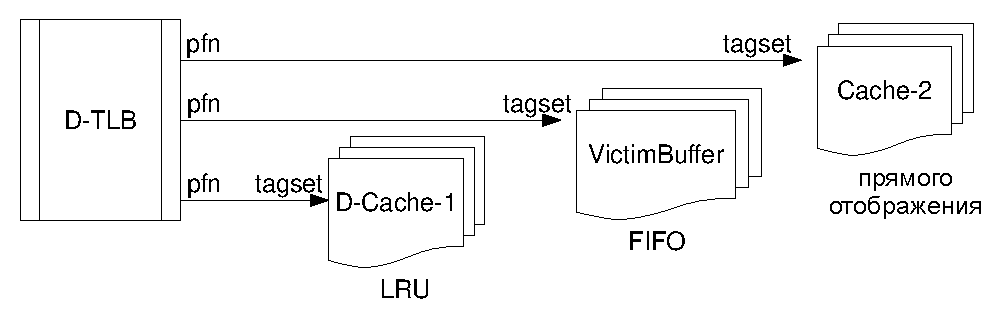
\includegraphics[width=0.8\textwidth]{4.analysis/alpha}\\
%  \caption{Схема MMU микропроцессора Alpha}\label{alpha_mmu_scheme}
%\end{figure}
%
%Совместная генерация возможна на границе TLB--кэш-память, так как
%получаемый из TLB номер физического кадра (pfn) становится битовым
%полем тегсета физического адреса (см.рис.~\ref{alpha_mmu_scheme}).



\section{Генерация тестов для архитектуры Pentium}

\begin{utv}
Для архитектуры Pentium возможно применение применение методов
генерации ограничений, описыванных в диссертации, для генерации
тестовых программ по тестовым шаблонам.
\end{utv}

Рассмотрим исполнение инструкции обращения к памяти в
микропроцессоре архитектуры Pentium P6. MMU в микропроцессорах
Pentium включает в себя (количественные характеристики приведены для
микропроцессора Intel Pentium III~\cite{HennessyPatterson3rd} -- см.
рис.~\ref{p6_mmu_scheme}):
\begin{itemize}
  \item \emph{кэш-память данных первого уровня (D-Cache-1)}: размер
  16 килобайт, наборно-ассоциативная, количество секций равно 2,
  стратегия вытеснения \LRU, размер строки 32 байта;
  \item \emph{кэш-память второго уровня (Cache-2)}: размер от 256 килобайт
  до 2 мегабайт, наборно-ассоциативная, количество секций равно 8, стратегия
  вытеснения \LRU, размер строки 32 байта;
  \item \emph{кэш-буфер TLB (D-TLB)}: наборно-ассоциативный,
  количество секций равно 4, в каждой секции 16 строк, стратегия вытеснения
  \PseudoLRU;
  \item \emph{таблица страниц виртуальной памяти (PageTable)}:
  размер страницы от 8 килобайт, длина логического адреса 48 бит,
  длина линейного адреса 32 бита, длина физического адреса 32 бита;
  \item \emph{таблица дескрипторов сегментов (SDT)}: размер от 8 байт до 64
  килобайт~\cite{FundamentalOfComputerOrganizationAndDesign}.
\end{itemize}
Таким образом, проблема возникнет при записи ограничений на
кэш-память и на TLB.

Инструкция может содержать тестовые ситуации в:
\begin{itemize}
  \item кэш-памяти данных первого уровня, первого и второго уровней;
  \item кэш-буфере данных TLB (D-TLB).
\end{itemize}

\begin{figure}[h] \center
  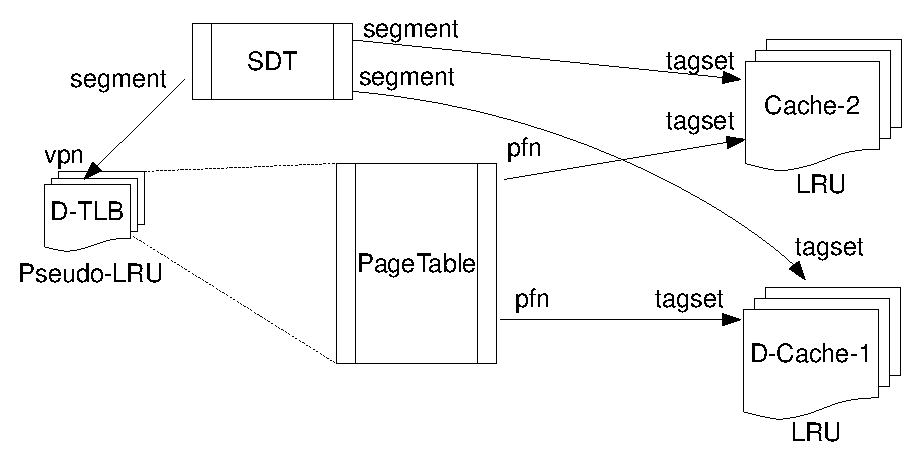
\includegraphics[width=0.8\textwidth]{4.analysis/p6}\\
  \caption{Схема MMU микропроцессора Pentium}\label{p6_mmu_scheme}
\end{figure}

Совместная генерация возможна (см. рис.~\ref{p6_mmu_scheme}):
\begin{itemize}
  \item на границе SDT--D-TLB, так как значение сегментного регистра
  становится битовым полем номера страницы виртуальной памяти (vpn);
  \item на границе D-TLB--кэш-память, так как получаемый из D-TLB номер
физического кадра (pfn) становится битовым полем тегсета физического
адреса;
  \item на границе SDT--кэш-память при неотображаемом обращении, так как
  получаемый из SDT сегментный регистр становится битовым полем тегсета физического
адреса.
\end{itemize}

\section{Оценка допустимой сложности тестовых шаблонов}

эксперименты с длинами и временем генерации/процентом успешной
генерации

\section{Сравнение с Genesys-Pro}
На рис.~\ref{comparison_genesyspro} показано сравнение предлагаемого
генератора тестовых программ с известным генератором
Genesys-Pro~\cite{GenesysPro}. Оба генератора получают на вход
тестовый шаблон, а на выходе у них тестовые программы.

Genesys-Pro на вход требует architectural model и testing knowledge
-- первая дает по сути эталонный симулятор микропроцессора (задает
операционную семантику инструкций и модель состояния
микропроцессора), а второй описывает эвристики выбора аргументов для
инструкции. Genesys-Pro чётко разделяет свойства аргументов
инструкции и свойства результата инструкции, соотношение между ними
задается не с помощью ограничений (т.е. не декларативным способом),
а в виде алгоритма (т.е. императивным способом). Genesys-Pro не
предполагает систематического описания семантики инструкций,
выделения ветвей их функциональности, описания программных
контрактов инструкций. Симулятор нужен для построения модельного
состояния микропроцессора после исполнения очередной сгенерированной
инструкции, а эвристики выбора аргументов составляют основу тех
ограничений, которые описывают значения аргументов очередной
инструкции.

Другой особенностью Genesys-Pro является то, что поддерживаемые им
тестовые шаблоны зачастую не фиксируют последовательность инструкций
(это позволяет строить более простые ограничения, потому как
генерируемая последовательность инструкций может по ходу генерации
подстраиваться под уже сгенерированные инструкции со
сгенерированными значениями аргументов, под состояние
микропроцессора, в которое привели сгенерированные инструкции).

Выразительный язык Genesys-Pro для описания ограничений однако
содержит такие нетривиальные конструкции, как явное использование
элементов массивов данных, что требует для разрешения продвинутый
решатель CSP, в том числе и заточенный под особенности генерации
тестовых данных для тестовых шаблонов (как минимум такие ограничения
могут включать битовые операции). Подобный решатель был разработан в
IBM для инструмента Genesys-Pro~\cite{GenesysSolver}. Однако
создание такого решателя -- отдельное сложное исследование, которое
не входило в цели данного исследования. В данной работе было принято
решение использовать доступные существующие решатели (не обязательно
CSP) и сосредоточиться на упрощении генерируемых ограничений для
некоторых частных случаев архитектур.

\begin{figure}[h]
\parbox{0.5\textwidth}{ \centering
  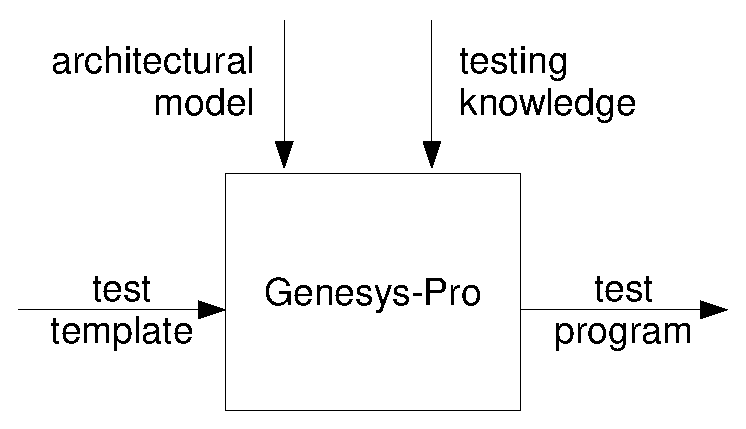
\includegraphics[width=0.45\textwidth]{3.impl/genesys-pro}
} \vline
\parbox{0.5\textwidth}{ \centering
  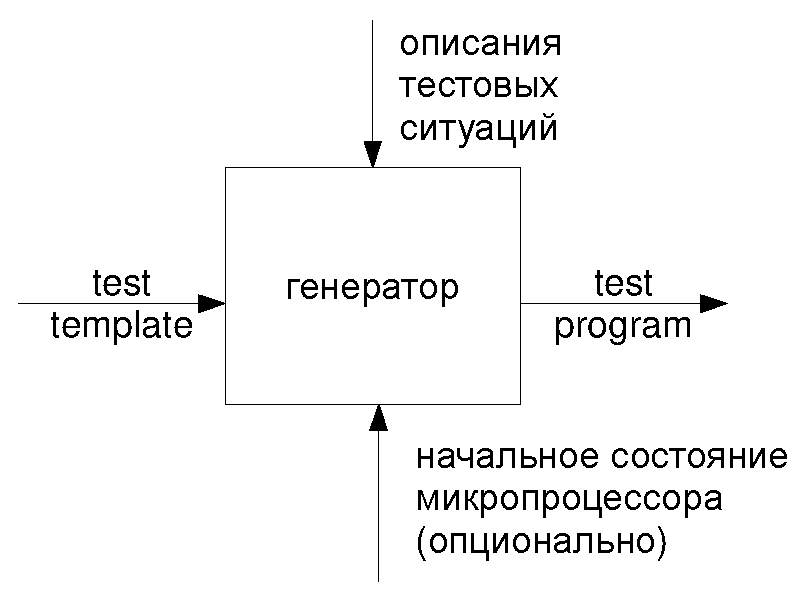
\includegraphics[width=0.45\textwidth]{3.impl/mygen}
}
\caption{Сравнение с Genesys-Pro}\label{comparison_genesyspro}
\end{figure}

В отличие от Genesys-Pro в предлагаемом инструменте описание
семантики инструкций задается в едином виде -- в виде описаний
тестовых ситуаций~\cite{my_syrcose_2008, my_isp_2008}. Каждая
тестовая ситуация описывает не только ограничение на свои аргументы,
но и результат исполнения инструкции \emph{при данном ограничении на
аргументы} инструкции декларативным образом. В функции, которую
реализует инструкция, выделяются отдельные \emph{ветви
функциональности}, ситуации различного поведения инструкций, каждая
ветвь функциональности становится отдельной тестовой ситуацией.
Например, инструкция целочисленного сложения ADD может быть
исполнена либо точно, либо с возникновением переполнения. Поэтому у
этой инструкции можно выделить 2 ветви функциональности (точное
исполнение и исполнение с переполнением), каждая ветвь дает свою
тестовую ситуацию. Кроме того, предлагаемый генератор дает
возможность указать начальное состояние микропроцессора, которое
будет эффективно использовано при построении тестовой программы.
Последовательность инструкций фиксирована и задается в тестовом
шаблоне.



%%%\section{��������}

��������������� �������� ����� �� ������ ������ ��������������
������. ������� ������������ ����������������, � ��� ����� � ��
��������� ������, �������� ���������� �������. ���������
�������������� ������������ ����������� � �������������� ��������
����� �������� �� ����� ���������� (�������� ��������). �����
��������� ����������� � ������ ������, �����������, ������� ��
���������� ��������������� � ����� �������������. � ����������
��������� �������, � ����� ������� �������������� ���� �����
����������� (������������ ��������� ���������, �������� �� ����, ���
�������� � ������������). ������ ��� ���������� ����������
������������ ��� ����������� ���������������� ��������� ���������
�������� ��������, ��� ������ ���������� ������ ��������������
��������� �������� ��������.

� ������~\cite{kamkin} ���������� ��������������� ������� ����������
�������� �������� �� ������ ������ ���������������. � ������ ����
������� ������� �������� ��������� �������������� �������� �
����������� ���� (� ���� ��������� �������) �- ��� ����������
���������� ����������. �������� ������� ��������� ������������������
����������, ��������� ���������� � ��������� ������������ �������
(��������, ������������, ������� ��� ��������� � ���-������). �
�������� ���������� ���������� ����� ���� ������� �������� �
���������. ������������������ ���������� ���� ����� ������ ����.
������������� � �������� ������� ������ ��������� �����, �����
������������ ���������� ���������� ������� � ��� ���� ��������
������������������� ����������, ������ �� ������� ������ ����
��������� �������� �������.

����� �������� �������� ��������� �� ��������� ��������� �������,
���������� ����� ��������� �������� ��������� � ��� ����� ���-������
� ������ ���������, � �������� �������� ���������� �������.
����������� � ������� ������ ���������� ��������� �������, � ������
�� ���������� � ������� ��������� �������� ������. �� ��������
������ �������� ����� ���������� ������������� ���������������
(�������� �������� � ��������, ��� � �.�.), ������� ����������� �
������ ��������� �������. ���������� ����� ������� ��������
��������� ����� ��������� � ���������, ��������� �� ��������� ������
���������� � ���, ��� ���� �������� � �������� �������. ��� �������
�������� �������� (������� �����������, ������� ������������������
����������) ������ ��������� �������� ������ ���������� ���������
���������, ������� � ��������� ������ ������.

%%%
%%%\section{����� ����� �� ���������� ��������������� ������������
����������������}

� ��������� ����� � �������� ���������� ��������������� ������������
���������������� ����� �������� ��������� ������� � ����������
�������� ��������:
\begin{itemize}
\item \emph{������ ���������� �������� ��������} ���� � ����������� �����������
��� ������� ������������ ���������������, �� �� ����� �����������
��� ������������ ������, ������� �������;
\item \emph{������������ � �������������� �����-����������} ����������� �����
��-�� ��������� ��������� ��� ����������: ����� ������������
������������ ��������������� ����� �������� ������ �����-����������,
� ���, ��������������� ��� �����-����������, ��� �����. ������
������������� ������� ����� ������������ �� �����;
\item \emph{��������� ��������� �������� ��������} ����������� ��� �� ����� �
���� �������� �������������. ��������������� ����� ������� ��������
��������� ��������� ������ ���������� ������� ������, ������ ��
����������� ������� ������������. ��������������� � ����� �������
�������� ��������� ���������~\cite{muGP};
\item \emph{��������� �������� �������� �� ������ ��������
��������} ������������ ���������� �������� ��������� ��������
��������� �� ��� ����� (��. ���.~\ref{pic_commonprocess}): �� ������
���������������� �������� ������� -- ����������� �������������
�������� �������� (� �������� �������� ��� ���������� ����������
������ �������� ����������� ����������� �� ��������) -- � �� ������
����� �� �������� �������� ������������ �������� ���������. ������
���� �������� � ���� \emph{��������� �������� ������}, �.�.
��������� ���������� ���������� (����������-��������) � ���������
�������� ���������, ����� ���-������, ����� TLB � �.�. ������ �����
��������� ��� ���������� �������� � �������� �������, � ������ �����
��������� ����� ������� ��������� �������� ������.
\end{itemize}

\begin{figure}
\center
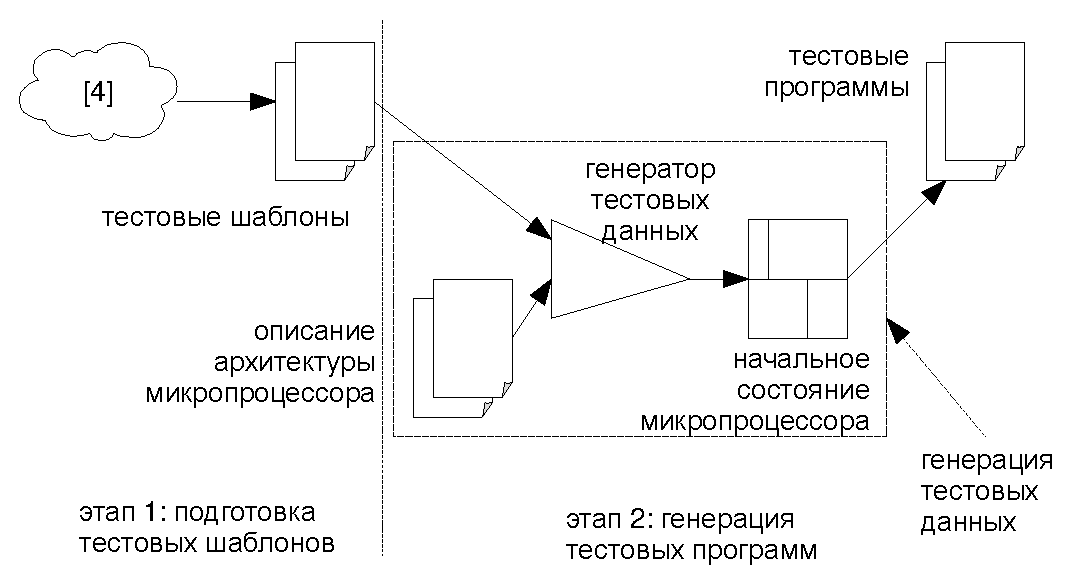
\includegraphics[width=0.8\textwidth]{test.eps}
\caption{��������� �������� �������� �� ������ ��������
��������}\label{pic_commonprocess}
\end{figure}

�������� ������� ��������� ������������������ ����������, ���������
���������� � ��������� ������������ ������� (��������, ������������,
������� ��� ��������� � ���-������). � �������� ����������
���������� ����� ���� ��� ���� ������� �������� � ���������, ��� �
������������� ����������� ����������� ������ ��������� ��������.
������������������ ���������� ���� ����� ������ ����. �������������
� �������� ������� ������ ��������� �����, ����� ������������
���������� ���������� ������� � ��� ���� ��������
������������������� ����������, ������ �� ������� ������ ����
��������� �������� �������. ������ ��������� �������:

{ \normalsize
\begin{verbatim}
REGISTER ax:32;
REGISTER bx:32;
REGISTER cx:32;
LW cx, ax, 0 @ l1Hit
SD ax, bx, 2 @ l1Miss
\end{verbatim}
}

\noindent � ���� �������� ������� 2 ���������� -- LW � SD. � ������
���������� ������� ��������� -- 2 �������� � ��������� -- � �����
����� '@' ���������� � ���, ��� ������ ���� ��������� ����������
(����������� �� �������� ���������� ���������� � ���������
���������������): l1Hit -- c ���-���������� (��� �������� �� ������
������ �� ���������� ����������� ������ � ������ ����������
���������� ������ �������������� � ���-������) � l1Miss -- c
���-�������� (��� �������� �� ������ ������ �� ����������
����������� ������ � ������ ���������� ���������� �� ������
�������������� � ���-������). ����� �������� �������� ��������� ��
����� �������, ���������� ������ ��������� �������� ��������� ax, bx
� cx � ��� ����� ���-������, � ������� �������� ����������
 -- ��� � ����� �������� ������ ��� ������� �������. ��� �����
�������, ������� � ������ ��������� ������� ���������� �������������
��������� ���������������. ���������� �������� ��������� �����
��������� � ���������, ��������� �� ��������� ������ ���������� �
���, ��� ���� �������� � �������� �������.

��������� � ������ ��������� �������� ������. ����� ��������� �����
����� �������� ��������� ������ �� �������:
\begin{itemize}
\item ������������� �������;
\item ������� ������ ATPG;
\item ���������� �����������.
\end{itemize}

\emph{������������� �������} ��������� � ������ ������� ��������
��������. ����� �������� ������� �������� ���� ������� �����������,
� ������ �������� ������� �������� ����������. ������ ��� ��������
���� ������� � �������� ��������� �����������. ������� ���� �
�������, �� �������� ������������ � ����������, ��������� �� ������
���������� �������� ����������� �� ���������� � ������ ��������
����. � ������ �������������� �� Fujitsu Lab.~\cite{TSE}
������������ ������� �������� ��������� � ���� ��������� (Test
Specification Expressions, TSE), � ���������� ��������������� -- ��
����� ISDL. ����������� ��������� ������ �������� ���������,
��������������� TSE. Kohno � Matsumoto~\cite{mVpGen} �������������
������ ����������� ����������� ����������������, ��������� ��� �����
��������� �������� �������� � ������� �������� ��������. �������
�������� ���������� � ����� �������� ������������ �� ��������� �
�������� ��������.

������������� �� Politecnico di Milano~\cite{toATPG} ����������
���������� �������� ������ � �������������� \emph{������ �������
������ ATPG} (Automatic Test Pattern Generation). ATPG -- ������
������ �������� ������� �������� (<<��������>>) ����� � ����� ������
�� ������������� ���������. ATPG ���� ����������� ��� ����������
������������, ���� �������� RTL-������ ���������������. ������ ATPG
�������� ����� � ��� �� ������� ���������� (� ��� �����
������������) �����������. ��� ���������� ATPG ��� ���������
�������� �������� ����������, ����� RTL-������ ��������������� ����
������ � ������� ��������� �������� ������. ����� ����,
������������� ����� �������� ������ ��� ��������������� ������������
����������, ��������� �������� ���������� �������������� �������
��������� ���������� -- ������� RTL-������ �������� ������,
�������������� ����������� � ��������� � ������� ��������������
����������� �� ���� ����������.

�������� ������������ ����������� ��������� �����������, ������������ ���
��������� �������� ������ \emph{���������� �����������}. ����������� �
���������� ����� ������ �� ��, ��� � ��������, � ������ ���������� �����������
-- �� ��, ��� � ������ ������������ ������� ����������, �� ��� ������� ����
������ ����������� ����������� ���������~\cite{ConstrProp}. �
������~\cite{MAATG} �������������� �� ���������� ������������� ������������
���������� ������������ ����������� ���������� MAATG. �������� ������ ��� ����
����� ��������� ���� ����������� ��������� ��� ����������� �������� � ��������
������� �������� ����������. ��� ������� ����������� ���������������
������������ �������� �� ����� EXPRESSION. ������ ���������� --
Genesys-Pro~\cite{GenesysPro2004} -- ��������������� ��������� IBM ���
����������, ��������� ������ �� ���������� ��������� 20 ���. �������� �������
��������� �������� �������� ��������� ���������� �����. ��� ����� ���������� �
�������� ������� ����� ���� ������� ��������� ��� ������ ��������
����������~\cite{GenesysPro2004Innovations}. ����� ��������� �������� ���� �
��������� �� ������� � ���-������ � ��� ���������� �������. ������ � ���������
������� �� ������������ ���������� ����� ��������, ��� �� ���� �����������
������ ������������� ��������� ��������, ���������� �� ������������ ������.
������� ������ ��������������� ������ ���� ������� � ���� �����������
(constraint net) �� ��������, ��� ��������, ��� �� �������� ������������
��������� ��������� ����������, �������� ���� � ������ ��� �����������
��������� ���������������� ���������� �� ������ ���������� ����������. ���
��������� ���������� ��������� ���������� Genesys-Pro ���������� ���
����������� �������� ��������� � ��������� ���������������, ������� ��������
���������. ���� ������ ��������� ���������������� �� ������� �������� �������,
�� � ������ � ������������� ������������� ��������� �������� (backtracking),
���� ������� ��������� ��� ��������� ���������� ����������.

%����� ���� ���������� �� ���������� """�������������� �����"""
%������ ������, � ���������� �������� ���������� ��������� �������,
%������ �� ��� ����������� ����� �������� ��������� �� ���� �������.
%����� �������, �������� ��������� �������� ��-��������, ��� �����
%������������ ��������� �� ������������� ������ Genesys-Pro ��
%������� �������� ��������.

% �� �������� ����� Genesys-Pro ���� ������ ��������� ��������� �������,
% � � ������ ����� ������� ������ - ����� ���������� ������������� �
% ��������� ���������! � IBM ��������� ������: ����� ������� - ���������
% ��������� ��� �������� (� �.�. ��� ����), � ��������� ������ "��������".
% ��������: cache = [ set1:0,5,10; set2:2,4,7 ], select(set,tag: cache miss)
% -> ������: set isin {1,2}, tag ~isin cache(set). ������ ������� ������ ��������,
% ����� ������. �������� set = 1, tag = 1. �� ������.
% � �������� ��� � ���, ��� � ����: (set,tag): cache miss,.... � ���!
% ��� ���� �������, ��� ����� miss.

� ������ ������ ��� ������� ������ ��������� �������� ������ �����
������������ ���������� �����������. ����������� ��� ������ � ������
��������������� ������� ���������� �������� �������� �� ������
������ ���������������~\cite{kamkin}. ������ ��� �������� ��������,
���������� � ������ ���� ��������������� �������, ���������� MAATG
����������, ��������� ������� ����� ��������� �� ������ �����������
��������� ��� ����������� ���������, �� � ����� ������� �����������,
��������, ���-������. � ������ ������ �� ��������� � Genesys-Pro
�������� ������ ������������� � ����������� ������� (��������, ���
������ ���������� ����������� (�.�. ������ ������������) NP-�����;
��� ��������, ��� ��� ������� �������� �������� ������������ �
������ ������ ����� ����� ���� �� ����� �����������, ������ ��������
����������, ��� ������ � ����������� ������ �������������� ��
�������� ���������� ��������� �����). ��� ������������ �����������
���������� ����������� �������� ������������� � ��������� ��������.
��-�� ����� ����������� �������� ����������� ������� �����������
(Genesys-Pro ������ ����� ������ � ��������� �����, �� �������
������� ���������). ����� ����, � ������ ������ ������������ �����
������������� ����� ���������� �������� ������: ������ ����������
��������������� ����� ���� �������� �� ��������� �����������
���������������.

������������ �������� ��������, ���������� � ������~\cite{kamkin}, ��������
�������� ��� ������ ���������� ���������-����������. ��� ����� ��������
Genesys-Pro ����� �������� ������ ������������, ��������� �������� �����������
� ������� ������ ���������� <<���������>> ���������� ��������� ���������� ���
�������� � �������� ������� ��� ��� �������. �� �������� ��������
��~\cite{kamkin} Genesys-Pro ����� �������� ��������� �������: �������
��������� ��������� ��������� ���������������, ������ ��������� �������� ������
(��������� ��������� ��������� ��� ��������), �� ��� ������ ������ ��
����������, ������� ����� ��������� �� ���, ��� ��������� � �������,
Genesys-Pro ������� ������� � ����� ������, � ������ ��� �������� �������
������ ��������� ��������� ��������������� � ���� ������� ��������� ������.
����� ������� ��������� �������� ������ ������� ������������. ��� ������� �����
���������� ������� � Genesys-Pro ������������ ������������ ������
DeepTrans~\cite{DeepTrans}. ������ �� ��������� ������� ���������� �������
����� � ���, ��� ����� ����� ���������� ������� ������������ � �����������.
������ ������ ���������� ��� �������� ������� ���������� ������ ��������
������� Memory � ������������ ���������. ��������, ��� ������� ����������
�����������, ����������� ������ � ���������� ������� ��� ����������� ��������,
�������� � ����� ������� ������������, ������������ ������� �� ���������� �����
����� ��������� ��� ��������.

������� �������� �������� ���� �� �������������� � ������ ������������
(����������� ��������� ��������� ������� �������� � ������������ ����� ���� �
���� �����������) ��� ���������� ������ � ������� �������� � ����� �������
������������, ������� �� ������� ��������� �� ���������� �����. ���� ��� �����
���������� ������� ��� ����������� ��������� ��������������� ����� ������������
������� ������ ������� ������� ������ ($mem_0 = var0 \wedge mem_1 = var1 \wedge
...$); ������ ��������� ������������ �� ������������ �������, ������� ���
������ ������ ��������� ��������������� ���������� ���������� ��� ���������
�������� ($mem[i] := x$ �������� � ������� $(i = 0 \wedge mem_0 = x \wedge
mem_1 = var1 \wedge ...) \vee (i = 1 \wedge mem_0 = var0 \wedge mem_1 = x
\wedge ...) \vee ...$), � ���� ����� ��������� ���������, �� ����������
������������� ��� ��������� �������� �������� ��������. ������������ �������
����� ������ ������� $|L| \cdot 2^n$, ��� $|L|$ -- ������ ������, � $n$ --
���������� ��������� ������. � ������ ������ ��������� ����� �����������
���������, ���������� � ������� ������� ������� $|L| + n$.

% ������� �� Genesys-Pro:
% 1) ������ �������� ��������� ��������� �������:
%    �������� ������ ��������������� �������, � �� �� ����� �������
% 2) ������ ���������� �������� ������ (��������, ���������� ���������)
%    �������� ����� �������. Genesys-Pro �� ���� ��, � �������� ������ �����
%    ������. ���� ������ �������, �����. � � ���� ������ �����.
% 3) ������������ ����� �������� �������� �������� ��������.
%    �� �����������, � ���������.
% 4) ���� ��������� ��������� ������ �������� ��������, ��������� ��� ���
%    ������� � ������������ �� �������� ����������� :)
% 5) Genesys-Pro �� �������� ��������, ��� ��� ����������� ���-�� ���������
%   (���, ��������, � ������� ��������), ����� �������� ������ ������������,
%   ��� ������������� ������ Genesys-Pro ����������� � �� ���� ����, ��� �� ���
%   ����� �������� ���������, ��������, ��������, ���� � ������� ��� ��������,
%   ����� ��� ������ ���� �������. �� ������� �������� Genesys-Pro �����������
%   ��������� ��������� ��������� ���������������, � ����� ������ ������ ���������
%   ������ (��������� � ������� �������� ��� �������� ��� �������). ����� ��������
%   �������� �������� - �� ���� ����� ������� Genesys-Pro. � ��� ���� ��� ����������
%   ��������� ������� �� ���������� ��������� �������� ��������, Genesys-Pro
%   ��������� � ������ ������ � ������� ������ ��������� ���������. ����� ��������
%   �������� ������. ���� �� ����������, ����� ������� � ����� ������ ���������� ��������.
%   ����� ����� ������������ � ����� ���������� ������!

%%%
%%%% !Mode:: "TeX:UTF-8"

\newcommand{\cmpn}[1]{\textsf{#1}}

\chapter{Описание предлагаемых методов и моделей}

\section{Описание предлагаемого подхода генерации тестовых программ}\label{sec:approach}

Рассмотрим следующую схему предлагаемого программного средства для генерации тестовой программы по тестовому шаблону (рисунок~\ref{fig:gen_scheme}). Программное средство изображено на схеме прямоугольником с подчеркнутыми границами. Внутри прямоугольника расположено 2 других прямоугольника, означающих следующие компоненты программного средства: \cmpn{Генератор ограничений} и \cmpn{Конструктор текстов программ}. На схеме есть прямоугольник \cmpn{Решатель ограничений} --- это другое программное средство, внешнее к программному средству для генерации тестовой программы. Остальные элементы схемы --- это исходные и выходные текстовые данные (тестовый шаблон, описания вариантов исполнения инструкций, описания устройств подсистемы управления памяти и тестовая программа), параллелограмм означает, что программное средство для генерации тестовой программы определило невозможность построения тестовой программы для данных исходных текстовых данных. Стрелки от текстовых данных к компонентам программного средства означают то, что эти текстовые данные являются входом компонентов. Стрелка от компонента \cmpn{Конструктор текстов программ} к тестовой программе означает то, что этот компонент строит тестовую программу. Стрелка от компонента \cmpn{Генератор ограничений} к \cmpn{Решатель ограничений}, подписанная словом <<ограничения>>, означает, что \cmpn{Генератор ограничений} строит ограничения, которые передаются как вход \cmpn{Решателю ограничений}. Стрелка от \cmpn{Решателя ограничений} к \cmpn{Конструктору текстов программ} означает то, что результат работы \cmpn{Решателя ограничений} становится входными данными компонента \cmpn{Конструктор текстов программ}.

\begin{figure}[h] \center
  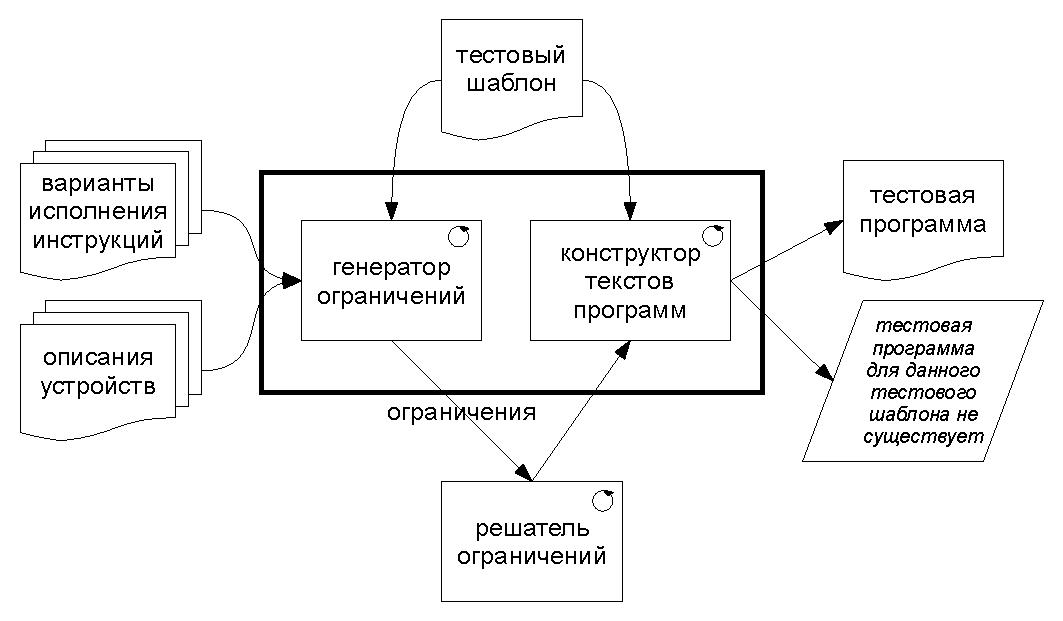
\includegraphics[width=0.8\textwidth]{2.theor/scheme}
  \caption{Программное средство для генерации тестовых программ}\label{fig:gen_scheme}
\end{figure}

Согласно схеме на рисунке~\ref{fig:gen_scheme} построение тестовой программы осуществляется следующим образом:
\begin{enumerate}
  \item \cmpn{Генератор ограничений} принимает на вход тестовый шаблон, описания вариантов исполнения инструкций и описания устройств подсистемы управления памяти и строит ограничения;
  \item Ограничения передаются на вход \cmpn{Решателю ограничений}; он определяет совместность данных ему ограничений; если ограничения несовместны, результатом его работы является сообщение о несовместности ограничений; если ограничения совместны, то он строит одно решение ограничений и сообщает это решение в качестве результата своей работы;
  \item \cmpn{Конструктор текстов программ} получает на вход тестовый шаблон и результат работы \cmpn{Решателя ограничений}; если \cmpn{Решатель ограничений} сообщил о несовместности ограничений, то \cmpn{Конструктор текстов программ} сообщает о несуществовании тестовой программы для данного тестового шаблона; иначе \cmpn{Конструктор текстов программ} на основе тестового шаблона по переданному \cmpn{Конструктору} решению ограничений строит тестовую программу, соответствующую тестовому шаблону.
\end{enumerate}

\begin{figure}[h] \center
  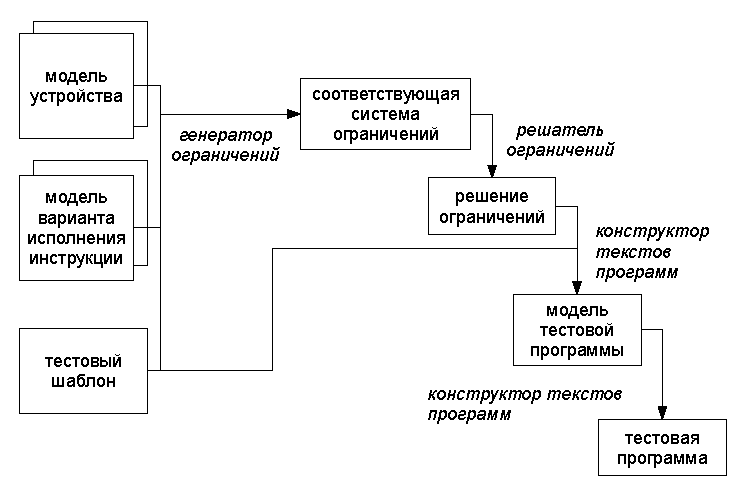
\includegraphics[width=0.8\textwidth]{2.theor/scheme2}
  \caption{Модели и задачи компонентов программного средства для генерации тестовых программ}\label{fig:models_tasks}
\end{figure}

Поставленная в разделе~\ref{sec:problem_refinement} задача решалась за счёт выбора специальных моделей (для вариантов исполнения инструкций, содержимого устройств подсистемы управления памяти и тестовой программы) и алгоритмов на основе этих моделей. На рисунке~\ref{fig:models_tasks} представлено место моделей в процессе генерации тестовой программы и задачи, которые решают компоненты описываемой здесь программной системы для генерации тестовых программ. В разделе~\ref{sec:state_model_section} будут даны формальные определения \emph{модели вариантов исполнения инструкций} и \emph{модели устройств}. В разделе~\ref{sec:constraints_generation_section} будет дано формальное определение \emph{системы ограничений, соответствующей} тестовому шаблону, моделям вариантов исполнения инструкций и моделям устройств. Неформально говоря, это такая система ограничений, которая эквивалентным образом выражает все ограничения на начальное состояние микропроцессора, содержащиеся в тестовом шаблоне и моделях. Задачей компонента \cmpn{Генератор ограничений} является построение системы ограничений, соответствующей тестовому шаблону, моделям вариантов исполнения инструкций и моделям устройств. Задачей \cmpn{Решателя ограничений} является разрешение этой системы ограничений. В разделе~\ref{?????} будет дано формальное определение \emph{модели тестовой программы} и \emph{модели тестовой программы, соответствующей решению ограничений и тестовому шаблону}. Неформально говоря, модель тестовой программы состоит из тестового шаблона, у каждой инструкции которого указаны значения ее аргументов, и последовательности адресов, по которым надо обратиться перед инструкциями тестового шаблона, и начальные значения регистров. Модель тестовой программы соответствует тестовому шаблону и решению ограничений, если в модели тестовой программы присутствует та же последовательность инструкций, а значения аргументов инструкций, адреса и начальные значения регистров взяты из решения ограничений. В разделе~\ref{????} будет дано формальное определение тестовой программы, соответствующей модели тестовой программы. Неформально говоря, это такая тестовая программа, которая исполняется в точном соответствии с моделью тестовой программы. Задачами компонента \cmpn{Конструктор тестовой программы} являются:
\begin{enumerate}
  \item построение модели тестовой программы, соответствующей тестовому шаблону и решению ограничений;
  \item построение тестовой программы, соответствующей модели тестовой программы.
\end{enumerate}




\section{Моделирование устройств подсистемы \\управления памяти и вариантов исполнения инструкций}\label{sec:state_model_section}

В данном разделе будут даны формальные определения ряда моделей%, будет уточнено определение тестового шаблона с учетом того, что эти шаблоны используются для тестирования подсистем управления памяти
. Будет дан ряд примеров и очерчена область применимости моделей.

\subsubsection*{Модель устройства подсистемы управления памяти}

%% определяется структура и содержание модельного состояния устройства

Назовем \emph{структурой поля} пару $(N, B)$, где $N$ --- произвольное имя, $B \in \mathds{N}$. $N$ будем называть \emph{именем} поля, $B$ --- \emph{битовой длиной} поля.

Назовем \emph{структурой строки} пару $(K, D)$, где $K$ и $D$ --- множества полей такие, что все поля в $K \cup D$ имеют разные имена. $K$ будем называть \emph{полями ключа}, $D$ будем называть \emph{полями данных}.

Назовем \emph{структурой региона} пару $(w, S)$, где $w \in \mathds{N}$, $S$ --- структура строки. $w$ будем называть \emph{ассоциативностью}.

Назовем \emph{структурной частью модели устройства} (или, \emph{структурой таблицы}) пару $(R, r)$, где $R \in \mathds{N} \cup \{0\}$, $r$ --- структура региона. Будем называть число $2^R$ \emph{количеством регионов}.

Назовем \emph{состоянием поля} со структурой $(N, B)$ целое число $v$ такое, что $v \geqslant 0$ и $v < 2^B$.

Назовем \emph{состоянием строки} со структурой $(K, D)$ пару $(k, d)$, где $K = \{K_1, K_2, ..., K_n\}$, $D = \{D_1, D_2, ..., D_m\}$, $k = \{k_1, k_2, ..., k_n\}$, $d = \{d_1, d_2, ..., d_m\}$, $k_i$ является состоянием поля $K_i$ для всех $i = 1, 2, ..., n$, $d_j$ является состоянием поля $D_j$ для всех $j = 1, 2, ..., m$.

Назовем \emph{состоянием региона} со структурой $(w, S)$ последовательность $\langle s_1,$ $s_2, ..., s_w\rangle$, где $r_i$ --- состояние строки со структурой $S$, $i = 1, 2, ..., w$, все состояния строк $s_j$ для $j = 1, 2, ..., w$ различные.

Назовем \emph{предикатом соответствия строки ключу} предикат $KM(k, \kappa)$, где $(k,d)$ --- состояние строки, $\kappa = (\kappa_1, \kappa_2, ..., \kappa_p)$, $\kappa_i \in \mathds{N} \cup \{0\}$, $i = 1, 2, ..., p$. Будем называть $\kappa$ \emph{ключом обращения}.

Назовем \emph{модельным состоянием устройства} со структурной частью $ST = (R, r)$ и предикатом соответствия строки ключу $KM$ последовательность $L = \langle r_0, r_1, ..., r_{2^R-1} \rangle$, где $r_i$ --- состояние региона со структурой $r$, $i = 0, 1, ..., 2^R{-}1$, и для любого состояния региона $r_i = \langle s_1, s_2, ..., s_w \rangle$ и для любого ключа обращения $\kappa$ не существует разных $s'$ и $s''$ из последовательности $r_i$ c состояниями полей ключей $k'$ и $k''$ соответственно таких, что $KM(k', \kappa)$ и $KM(k'', \kappa)$ истинны.


%% далее определяем правильные цепочки состояний
%%    с помощью определения правильных переходов между состояниями
%% > в результате будет определена `стратегия вытеснения'

Далее определим понятие <<стратегии вытеснения>> и ряда функций над модельными состояниями устройств.

Функция $hit: S \times \kappa \rightarrow S$, где $S$ --- состояние региона, $\kappa$ --- ключ обращения, определенная на тех парах $(S, \kappa)$, что в $S$ есть состояние строки $s = (k,d)$ такое, что $KM(k, \kappa)$ истинно, причем множество состояний строк в $hit(S, \kappa)$ и в $S$ одинаковые. Будем говорить, что в функции $hit$ осуществляется \emph{обращение к строке} $s$.

Функция $load: S \times \kappa \times dL \rightarrow S$, где $S$ --- состояние региона, $\kappa$ --- ключ обращения, $dL$ --- состояние полей данных, определенная на тех тройках $(S, \kappa, dL)$, что в $S$ есть состояние строки $s = (k,d)$ такое, что $KM(k, \kappa)$ истинно и $d = dL$, причем $load(S, \kappa, dL) = hit(S, \kappa)$. Будем говорить, что в функции $load$ осуществляется \emph{обращение к строке} $s$.

Функция $store: S \times \kappa \times dS \rightarrow S$, где $S$ --- состояние региона, $\kappa$ --- ключ обращения, $dS$ --- состояние полей данных, определенная на тех тройках $(S, \kappa, dS)$, что в $S$ есть состояние строки $s = (k,d)$ такое, что $KM(k, \kappa)$ истинно, причем выполнено следующее свойство: обозначим $store(S, \kappa, dS) = \langle r'_0, r'_1, ..., r'_{2^R-1}\rangle$ и $hit(S, \kappa) = \langle r''_0, r''_1, ..., r''_{2^R-1}\rangle$, $r''_i = s$, тогда $r'_j = r''_j$ для $j = 0, 1, ..., 2^R{-}1$, $j \neq i$, $r'_i = (k, dS)$. Будем говорить, что в функции $store$ осуществляется \emph{обращение к строке} $s$.

Функция $miss: S \times \kappa \rightarrow S$, где $S$ --- состояние региона, $\kappa$ --- ключ обращения, определенная на тех парах $(S, \kappa)$, что в $S$ нет состояния строки $s = (k,d)$ такого, что $KM(k, \kappa)$ истинно, и $miss(S, \kappa) = S$.

Назовем \emph{правилом определения вытесняемой строки} функцию $EV : S \rightarrow s$, где $S$ --- состояние региона, $s$ является состоянием одной из строк в $S$.

Функция $replace: S \times \kappa \times dR \rightarrow S$, где $S$ --- состояние региона, $\kappa$ --- ключ обращения, $dR$ --- состояние полей данных, определенная на тех тройках $(S, \kappa, dR)$, что в $S$ нет состояния строки $s = (k,d)$ такого, что $KM(k, \kappa)$ истинно, в состоянии региона $replace(S, \kappa, dR)$ есть состояние строки $s' = (\kappa, dR)$ и множество состояний строк в $S$ без состояния строки $EV(S)$ равно множеству состояний строк в $replace(S, \kappa, dR)$ без $s'$.

Назовем \emph{стратегией вытеснения} тройку функций $(hit, replace, EV)$.

Далее определим ряд семейств бинарных отношений над модельными состояниями устройств (другими словами, определим ряд \emph{параметризованных} бинарных отношений над модельными состояниями устройств, это означает, что каждому отношению будет сопоставлен ряд чисел и векторов чисел). Все определяемые далее бинарные отношения должны быть функциями, т.е. они должны определять однозначное соответствие (но не обязательно взаимно однозначное соответствие). По этой причине эти отношения будут далее в том числе использоваться как \emph{операции} над модельным состоянием.

Назовем \emph{отношением успешного обращения без данных} $Hit_{\kappa, \rho}$ множество пар модельных состояний $(L', L'')$, где $\kappa$ --- ключ обращения, $\rho$ --- целое число, $L' = \langle r'_0, r'_1, ..., r'_{2^R-1} \rangle$, $L'' = \langle r''_0, r''_1, ..., r''_{2^R-1} \rangle$, в которых выполнены все 3 следующие свойства:
  \begin{enumerate}
    \item $r''_i = r'_i$ для $i = 0, 1, 2, ..., 2^R{-}1$, $i \neq \rho$;
    \item в состоянии региона $r'_{\rho}$ существует строка $s = (k,d)$, для которой истинно $KM(k, \kappa)$;
    \item $r''_{\rho} = hit(r'_{\rho}, \kappa)$.
  \end{enumerate}

Назовем \emph{отношением успешного обращения с данными без изменения} (или, просто, \emph{отношением успешного обращения}) $HitLoad_{\kappa, \rho, dL}$ множество пар модельных состояний $(L', L'')$, где $\kappa$ --- ключ обращения, $\rho$ --- целое число, $dL$ --- состояние полей данных, $L' = \langle r'_0, r'_1, ..., r'_{2^R-1} \rangle$, $L'' = \langle r''_0, r''_1, ..., r''_{2^R-1} \rangle$, в которых выполнены все 3 следующие свойства:
  \begin{enumerate}
    \item $r''_i = r'_i$ для $i = 0, 1, 2, ..., 2^R{-}1$, $i \neq \rho$;
    \item в состоянии региона $r'_{\rho}$ существует строка $s = (k,d)$, для которой истинно $KM(k, \kappa)$ и $d = dL$;
    \item $r''_{\rho} = load(r'_{\rho}, \kappa, dL)$.
  \end{enumerate}

Назовем \emph{отношением успешного обращения без данных с изменением}\\ $HitStore_{\kappa, \rho, dS}$ множество пар модельных состояний $(L', L'')$, где $\kappa$ --- ключ обращения, $\rho$ --- целое число, $dS$ --- состояние полей данных, $L' = \langle r'_0, r'_1, ..., r'_{2^R-1} \rangle$, $L'' = \langle r''_0, r''_1, ..., r''_{2^R-1} \rangle$, в которых выполнены все 3 следующие свойства:
  \begin{enumerate}
    \item $r''_i = r'_i$ для $i = 0, 1, 2, ..., 2^R{-}1$, $i \neq \rho$;
    \item в состоянии региона $r'_{\rho}$ существует строка $s = (k,d)$, для которой истинно $KM(k, \kappa)$;
    \item $r''_{\rho} = store(r'_{\rho}, \kappa, dS)$.
  \end{enumerate}

Назовем \emph{отношением успешного обращения с данными с изменением} (или, просто, \emph{успешного обращения с изменением}) $HitLoadStore_{\kappa, \rho, dL, dS}$ множество пар модельных состояний $(L', L'')$, где $\kappa$ --- ключ обращения, $\rho$ --- целое число, $dL$ и $dS$ --- два состояния полей данных устройства, $L' = \langle r'_0, r'_1, ..., r'_{2^R-1} \rangle$, $L'' = \langle r''_0, r''_1, ..., r''_{2^R-1} \rangle$, в которых выполнены все 3 следующие свойства:
  \begin{enumerate}
    \item $r''_i = r'_i$ для $i = 0, 1, 2, ..., 2^R{-}1$, $i \neq \rho$;
    \item в состоянии региона $r'_{\rho}$ существует строка $s = (k,d)$, для которой истинно $KM(k, \kappa)$ и $d = dL$;
    \item $r''_{\rho} = store(r'_{\rho}, \kappa, dS)$.
  \end{enumerate}

Назовем \emph{отношением неуспешного обращения без замещения} $Miss(\kappa, \rho)$ множество пар модельных состояний $(L', L'')$, где $\kappa$ --- ключ обращения, $\rho$ --- целое число, $L' = \langle r'_0, r'_1, ..., r'_{2^R-1} \rangle$, $L'' = \langle r''_0, r''_1, ..., r''_{2^R-1} \rangle$, в которых выполнены все 3 следующие свойства:
  \begin{enumerate}
    \item $r''_i = r'_i$ для $i = 0, 1, 2, ..., 2^R{-}1$, $i \neq \rho$;
    \item в состоянии региона $r'_{\rho}$ нет состояния строки $s = (k,d)$, для которой истинно $KM(k, \kappa)$;
    \item $r''_{\rho} = miss(r'_{\rho}, \kappa)$.
  \end{enumerate}

Назовем \emph{отношением неуспешного обращения с замещением}\\ $MissReplace(\kappa, \rho, dR)$ множество пар модельных состояний $(L', L'')$, где $\kappa$ --- ключ обращения, $\rho$ --- целое число, $dR$ --- состояние полей данных, $L' = \langle r'_0, r'_1, ...,$ $r'_{2^R-1} \rangle$, $L'' = \langle r''_0, r''_1, ..., r''_{2^R-1} \rangle$, в которых выполнены все 3 следующие свойства:
  \begin{enumerate}
    \item $r''_i = r'_i$ для $i = 0, 1, 2, ..., 2^R{-}1$, $i \neq \rho$;
    \item в состоянии региона $r'_{\rho}$ нет строки $s = (k,d)$, для которой истинно $KM(k, \kappa)$;
    \item $r''_{\rho} = replace(r'_{\rho}, \kappa, dR)$.
  \end{enumerate}


Назовем \emph{моделью устройства} (или, \emph{таблицей}) тройку $(ST, RP, KM)$, где $ST$ --- структурная часть модели устройства, $RP$ --- стратегия вытеснения, $KM$ --- предикат соответствия строки ключу.

%% теперь вводим конечный автомат, раз он фигурирует в результатах автореферата!

Из введенной модели устройства следует представление устройства подсистемы управления памяти \emph{в виде конечного автомата}. Множеством состояний такого конечного автомата является множество всех модельных состояний (так, как они определены выше) и состояние Fail. Одно из модельных состояний выбрано в качестве начального состояния. Неформально говоря, к устройству производятся <<обращения>> с целью загрузить данные из устройства по заданному ключу в заданном регионе или сохранить данные в устройстве по заданному ключу в заданному регионе. Каждому обращению будет соответствовать один переход в конечном автомате. Переход помечен символом load, если это обращение с целью загрузки данных, или символом store, если это обращение с целью сохранения данных. Кроме того, символы load и store снабжены параметрами. load снабжен двумя параметрами: $\kappa$ (ключом обращения) и $\rho$ (номером региона). store снабжен тремя параметрами: $\kappa$ (ключом обращения), $\rho$ (номером региона) и $\delta$ (состоянием полей данных). Выходной алфавит конечного автомата состоит из символов $HitLoad$, $HitStore$ и $MissReplace$. Символ $HitLoad$ снабжен параметром $\delta$ (состояние полей данных). Функция переходов конечного автомата определено соответственно определениям отношений $HitLoad$, $HitStore$ и $MissReplace$, а именно:
  \begin{itemize}
    \item если для модельного состояния $L'$ существует такое модельное состояние $L''$, что $(L', L'') \in Hit_{\kappa, \rho}$, то из состояния $L'$ по входу load$(\kappa, \rho)$ осуществляется переход в состояние $L''$, при этом выходом является $HitLoad(\delta)$, где $\delta$ --- состояние полей данных такое, что $(L', L'') \in HitLoad_{\kappa, \rho, \delta}$; такой переход будет называться далее \emph{успешным обращением без изменения} (или, просто, \emph{успешного обращения});
    \item если для модельного состояния $L'$ не существует модельное состояние $L''$ такое, что $(L', L'') \in Hit_{\kappa, \rho}$, то из состояния $L'$ по входу load$(\kappa, \rho)$ осуществляется переход в состояние Fail;
    \item если для модельного состояния $L'$ существует такое модельное состояние $L''$, что $(L', L'') \in HitStore_{\kappa, \rho, \delta}$, то из состояния $L'$ по входу store$(\kappa, \rho, \delta)$ осуществляется переход в состояние $L''$, при этом выходом является\\ $HitStore$; такой переход будет называться далее \emph{успешным обращением c изменением};
    \item если для модельного состояния $L'$ существует такое модельное состояние $L''$, что $(L', L'') \in MissReplace_{\kappa, \rho, \delta}$, то из состояния $L'$ по входу store$(\kappa, \rho, \delta)$ осуществляется переход в состояние $L''$, при этом выходом является $MissReplace$; такой переход будет называться далее \emph{неуспешным обращением};
    \item все переходы из Fail ведут в Fail.
  \end{itemize}

Из определения отношений $HitStore$ и $MissReplace$ следует, что для любых $\kappa$, $\rho$, $\delta$ и для любого состояния $L'$, отличного от Fail, всегда есть либо переход из $L'$, помеченный $HitStore(\kappa, \rho, \delta)$, либо переход из $L'$, помеченный $MissReplace(\kappa, \rho, \delta)$.

Введенный таким образом конечный автомат позволяет по цепочке обращений в устройство из некоторого состояния определить, является ли эта цепочка обращений допустимой (т.е. приводит ли она в состояние Fail) и какие из обращений в этой цепочке были успешными, а какие были неуспешными.

% примеры моделей для устройств давать не буду, т.к. слишком много надо пояснять (почему LRU моделируется таким способом, почему регионы с вытеснением - это строки секций по одному и тому же индексу и т.д.)
% но можно ли тут сказать, что эту модель можно построить для практически полезных устройств? (кэш-память, TLB в MIPS, оперативная память)

% нотация
Для программной системы построения тестовых программ по тестовым шаблонам устройство подсистемы управления памяти должно быть представлено в рамках определенной в этом разделе модели устройства. Модель должна быть записана в виде \emph{описания устройства}. Описание устройства состоит из предиката соответствия строки ключу keyMatch и из пар <<название параметра = значение параметра>> для следующих параметров:
\begin{itemize}
    \item policy --- идентификатор, представляющий стратегию вытеснения (\LRU, \FIFO, \PseudoLRU); в число этих идентификаторов добавлен идентификатор none, он означает такую <<стратегию вытеснения>>, в которой нет функции replace и, соответственно, нет отношения $MissReplace$ (этот частный случай удобен при моделировании оперативной памяти, где отношения $Miss$ и $MissReplace$ по определению невозможны и при моделировании устройств, в которых неуспешные обращения не приводят к замещению);
    \item regionbits --- первый компонент структурной части модели устройства (двоичный логарифм количества регионов);
    \item lines --- количество строк в регионе (первый компонент структуры региона);
    \item line --- структура строки (для каждого поля указывается название, битовая длина, поле ли это ключа или поле данных).
%    \item keyMatch --- предикат от аргументов операции обращения и полей ключа строки; он истинен в том и только том случае, когда строка соответствует аргументам операции (тегам физического адреса, номерам виртуальных страниц и т.п.).
\end{itemize}

Пример описания кэш-памяти:
\begin{verbatim}
table L1 {
  policy = LRU;
  regionbits = 7;
  lines = 4;
  line( tag:24:key, d:32:data );
  keyMatch(kappa_tag:24) { kappa_tag = tag };
}
\end{verbatim}

Строка кэш-памяти состоит из поля tag, оно является полем ключа, и поля d. Ключ обращения состоит из одного компонента (kappa\_tag), его битовая длина равна 24 (т.е. kappa\_tag принимает целые значения от 0 до $2^{24}{-}1$. Ключ обращения соответствует строке, если kappa\_tag равен полю tag. Стратегия вытеснения LRU определяет такие правила перестановки строк, что в функции $replace$ замещается строка, последнее обращение к которой произошло раньше последнего обращения к любой другой строке региона. Детальное рассмотрение этой и других стратегий вытеснения будет сделано в разделе~\ref{sec:policy_table}.

%%% нужны пояснения ???

%Рассуждая для кэш-памяти (ее структура описана в разделе~\ref{section:cache}), строками будут кэш-строки с тегами адресов. Регион будут составлять кэш-строки из всех секций, расположенные по одному и тому же индексу. Количество строк в регионе  равно количеству секций, т.е. ассоциативности кэш-памяти $w$. Количество регионов равно количеству кэш-строк в секции.
%
%Буфер трансляции (TLB) в микропроцессорах архитектуры MIPS64~\cite{mips64III} состоит из строк, каждая строка содержит ряд полей, в том числе половину номера виртуальной страницы $v$, номер физического кадра, соответствующего виртуальной странице с номером $2v$, и номер физического кадра, соответствующего виртуальной странице с номером $2v+1$. Обращение в буфер происходит по некоторому виртуальному адресу. Если его половина присутствует в одной из строк TLB, то вычисляется физический адрес на основе одного из номеров физических кадров той же строки. Эту ситуацию будем считать <<попаданием>>. Если его половине не присутствует ни в одной из строк TLB, ситуацию будем считать <<промахом>>. При этом одна из строк будет вытеснена и заменена другой (это делается программно так же, как показано на рисунке~\ref{fig:blocks_init_examples}. Поэтому буфер трансляции адресов в микропроцессорах архитектуры
%MIPS64 моделируется таблицей из одного региона, каждая его строка состоит из полей \texttt{r}, \texttt{vpn/2}, \texttt{g}, \texttt{asid}, \texttt{pfn}$_0$, \texttt{CCA}$_0$, \texttt{v}$_0$, \texttt{pfn}$_1$, \texttt{CCA}$_1$, \texttt{valid}$_1$ и других.
%
%Упор на вытеснение сделан неслучайно: как показано в разделе~\ref{section:cache}, ряд важных ошибок связан именно с некорректной реализацией вытеснения. Предлагаемые здесь модели составляются для устройств подсистемы управления памяти, обладающих вытеснением. Это кэш-память всех уровней, таблицы трансляции адресов. Таким же образом можно смоделировать и оперативную память: строка такой таблицы содержит физический адрес и данные по нему, каждый регион состоит из одной строки.

%Описание модели уже упомянутого буфера трансляции адресов микропроцессоров архитектуры
%MIPS64 выглядит следующим образом:
%\begin{verbatim}
%table TLB
%{
%    line(   r:2:key, vpnd2:28:key, g:1:key, asid:4:key,
%            pfn0:24:data, cca0:3:data, valid0:1:data,
%            pfn1:24:data, cca1:3:data, valid1:1:data );
%    regionbits = 0;
%    policy = none;
%    lines = 48;
%    keyMatch(r:2, vpnd2:28) { .... };
%}
%\end{verbatim}
%
%Предикат keyMatch будет приведен чуть позже, когда будет описан для этого язык.




\subsubsection*{Модель варианта исполнения инструкций}

Напомню, что вариант исполнения инструкции --- это ограничение на значения аргументов инструкции и состояния микропроцессора, перед инструкцией и после нее.

%Здесь будет дано определение модели варианта исполнения инструкции.

%Представление варианта исполнения инструкции в рамках этой модели позволит увеличить при автоматизации построения тестовой программы для тестового шаблона

Назовем \emph{моделью варианта исполнения инструкции} для моделей устройств $M_1, M_2, ..., M_n$ пятерку $(Y, X, U, P, S)$, где
  \begin{itemize}
    \item $Y$ --- конечное множество переменных (множество \emph{выходных переменных});
    \item $X$ --- конечное множество переменных (множество \emph{входных переменных}), $X \cap Y = \varnothing$;
    \item $U$ --- конечное множество переменных (множество \emph{промежуточных переменных}), $U \cap Y = \varnothing$, $U \cap X = \varnothing$;
    \item $P$ --- ограничение над переменными $X \cup Y \cup U$;
    \item $S$ --- это множество троек $(M, r, p)$, где $M \in \{M_1, M_2, ..., M_n\}$, $r \in \{Hit,$ $HitLoad, HitStore, HitLoadStore, Miss, MissReplace\}$, $p$ --- это либо пара $(\kappa, \rho)$ при $r \in \{Hit, Miss\}$, либо тройка $(\kappa, \rho, d)$ при $r \in \{HitLoad,$ $HitStore, MissReplace\}$, либо четверка $(\kappa, \rho, dL, dS)$ при $r = HitLoadStore$, $\kappa$, $d$, $dL$, $dS$ --- последовательности переменных из множества $X \cup Y \cup U$, $\rho \in X \cup Y \cup U$, причем нет двух троек с одинаковым компонентом $M$.
  \end{itemize}

Тем самым модель указывает, что в рамках варианта исполнения инструкции допустим лишь определенный вид изменения модельного состояния устройств ($Hit$, $HitLoad$, $HitStore$, $HitLoadStore$, $Miss$ и $MissReplace$).

% нотация и семантика
Как и модели устройств, модели вариантов исполнения инструкций должны быть описаны на специальном языке для их использования в программной системе построения тестовых программ. Грамматика языка описания вариантов исполнения инструкции в виде расширенной формы Бэкуса-Наура приведена в приложении~\ref{sec:syntax}. Описание варианта исполнения инструкции состоит из двух частей: заголовка и тела описания. Заголовок состоит из объявлений аргументов инструкции. Объявление аргумента состоит из имени внутри данного описания и битовой длины аргумента. Аргументы в описаниях вариантов исполнения инструкций аналогичны формальным параметрам процедур в языке Паскаль с передачей аргументов по ссылке. Тело описания варианта исполнения инструкции состоит из последовательности \emph{операторов} над переменными-битовыми строками (let, assume) и операторов-обращений (hit, miss). Операторы над переменными-битовыми строками задают ограничение $P$, а операторы-обращения задают последовательность $\langle (r_i, p_i) \rangle_{i=1}^n$ (обозначения из определения модели варианта исполнения инструкции).

Семантика описаний вариантов исполнения инструкций представлена на языке RSL~\cite{RSL} в приложении~\ref{sec:semantics}. Назовем \emph{допустимым модельным состоянием} для модели варианта исполнения инструкции $(Y, X, U, P, S)$ вектор из значений всех переменных множества $X \cup Y \cup U$ и для каждой модели устройств подсистемы управления памяти бесконечная последовательность модельных состояний с указанием на одно из модельных состояний как на <<текущее>>. Каждому оператору в описании варианта исполнения инструкции сопоставим пару множеств допустимых модельных состояний $(PreS, PostS)$, причем $PostS \subseteq PreS$. Множество $PostS$ для произвольного (не последнего) оператора в описании варианта исполнения инструкции равно множеству $PreS$ для следующего оператора в этом же описании варианта исполнения инструкции. В приложении~\ref{sec:semantics} на языке RSL дано формальное определение допустимого модельного состояния и отношений над парами множеств допустимых модельных состояний $(PreS, PostS)$ для каждого оператора. Далее будут рассмотрены эти отношения для каждого оператора.

По определению множество допустимых модельных состояний $PostS$ последнего оператора в описании варианта исполнения инструкции включает лишь те модельные состояния устройств подсистемы управления памяти и значения переменных, из которых выполнены все операторы описания варианта исполнения инструкции. Если $PreS$ первого оператора в описании варианта исполнения инструкции включает все возможные допустимые модельные состояния, то $PostS$ последнего оператора этого описания варианта исполнения инструкции включает те и только те модельные состояния, на которых выполнены все операторы варианта исполнения инструкции. Описанию варианта исполнения инструкции соответствуют 2 множества допустимых модельных состояний: $PreS$ первого оператора в этом варианте исполнения инструкции и $PostS$ последнего оператора того же варианта исполнения инструкции. В тестовом шаблоне описания вариантов исполнения инструкций расположены в заданной последовательности, в которой $PostS$ для произвольного (не последнего) варианта исполнения инструкции совпадает с $PreS$ следующего за ним варианта исполнения инструкции. Тем самым, если $PreS$ первого описания варианта исполнения инструкции включает все возможные допустимые модельные состояния, то $PostS$ последнего описания варианта исполнения инструкции включает те и только те допустимые модельные состояния, на которых выполнены все варианты исполнения инструкции --- каждое такое допустимое модельное состояние задает \emph{начальное} состояний микропроцессора, из которого инструкции тестового шаблона будут исполняться согласно указанным вариантам исполнения. В это начальное состояние микропроцессора входят значения переменных, соответствующих регистрам микропроцессора, и первые элементы в последовательностях модельных состояний устройств.

$PostS$ \emph{оператора допущения} (\texttt{assume : boolexpr;}) равно множеству тех состояний из $PreS$, в которых для значений переменных выполнено логическое выражение \texttt{boolexpr}.

Входные и выходные переменные должны быть объявлены в заголовке описания варианта исполнения инструкции. А промежуточные переменные появляются внутри описаний вариантов исполнения инструкции --- для этого служит \emph{оператор объявления нового имени} let. Этот оператор имеет две формы: явную (\texttt{var <- expr;}) и неявную (\texttt{let var : BITLEN;}), \texttt{var} --- это имя переменной, \texttt{expr} --- выражение, \texttt{BITLEN} --- натуральное число. Оператор let в неявной форме объявляет промежуточную переменную \texttt{var} (т.е. в операторах описания варианта исполнения инструкции, расположенных до этого оператора let, переменной \texttt{var} нельзя пользоваться, после этого оператора --- можно) и фиксирует битовую длину ее значений, т.е. переменная может принимать любое целое значение от 0 до $2^{\mbox{\texttt{BITLEN}}}-1$. Иными словами, для оператора let в неявной форме $PostS$ равно $PreS$, причем все модельные состояния из $PostS$ отличаются лишь значением переменной \texttt{var} и среди всех модельных состояний из $PostS$ переменная \texttt{var} принимает все целые значения от 0 до $2^{\mbox{\texttt{BITLEN}}}-1$. Оператор let в явной форме является краткой записью такой последовательности операторов: \texttt{let var: BITLEN; assume: var = expr;}.

Операторам-обращения соответствуют следующие отношения над парами множеств модельных состояний $(PreS, PostS)$:
\begin{itemize}
  \item $PostS$ \emph{оператора попадания} \texttt{hit<table>(key, region) \{[loaded(} \\ \texttt{datafields)] [storing(datafields)]\}} равно множеству тех состояний из $PreS$, в которых текущее модельное состояния устройства table и следующее за ним модельное состояние устройства table находятся в отношении $p \in \{Hit, HitLoad, HitStore, HitLoadStore\}$, в этих отношениях состояние полей ключа $\kappa$ равно значению выражения \texttt{key} от значений переменных в допустимом модельном состоянии, а значение номера региона $\rho$ равно значению выражения \texttt{region} от значений переменных в допустимом модельном состоянии; синтаксис оператора попадания допускает наличие и отсутствие \texttt{loaded(datafields)} и \texttt{storing(datafields)}; если эти обе части отсутствуют, то $p = Hit$, если присутствует только \texttt{loaded}, то $p = HitLoad$, если присутствует только \texttt{storing}, то $p = HitStore$, в противном случае $p = HitLoadStore$, $datafields$ --- это последовательность выражений, задающая состояние полей данных;
  \item $PostS$ \emph{оператора промаха} \texttt{miss<table>(key, region) \{[replacing(} \\ \texttt{datafields)]\}} равно множеству тех состояний из $PreS$, в которых текущее модельное состояния устройства table и следующее за ним модельное состояние устройства table находятся в отношении $p \in \{Miss,$ $MissReplace\}$, в этих отношениях состояние полей ключа $\kappa$ равно значению выражения \texttt{key} от значений переменных в допустимом модельном состоянии, а значение номера региона $\rho$ равно значению выражения \texttt{region} от значений переменных в допустимом модельном состоянии; синтаксис оператора попадания допускает наличие и отсутствие \texttt{replacing(}\\ \texttt{datafields)}; в случае отсутствия \texttt{replacing} $p = Miss$, в противном случае $p = MissReplace$, $datafields$ --- это последовательность выражений, задающая состояние полей данных.
\end{itemize}

Неформально говоря, вариант исполнения инструкции описывается как последовательность уточнений состояния (assume), объявлений новых переменных (let) и обращений к устройствам подсистемы управления памяти (hit, miss).

Для составления выражений boolexpr и expr определены следующие <<операции>>~\cite{my_syrcose_2008, my_isp_2008}:
\begin{itemize}
    \item битовые операции:
        \begin{itemize}
            \item выделение бита с заданным индексом: \texttt{x[i]} есть значение \texttt{i}'го бита битовой строки \texttt{x};
            \item выделение диапазона бит в заданных границах: \texttt{x[i..j]} есть битовая строка, составленная из последовательности бит строки \texttt{x} с номерами \texttt{i}, \texttt{i+1}, ..., \texttt{j};
            \item битовая конкатенация: \texttt{x || y} есть битовая строка, первые биты которой равны битам строки \texttt{x}, а последующие --- битам строки \texttt{y};
            \item битовая степень: \texttt{x\^{ }n} есть битовая строка, равная $\underbrace{\mbox{\texttt{x||x||...||x}}}_{\mbox{\texttt{n}}}$;
            \item знаковое расширение битового размера: \texttt{(n) x} есть строка, битовая длина которой равна \texttt{n} и в знаковом представлении значение этой строки совпадает со значением строки \texttt{x};
        \end{itemize}
    \item арифметические операции (суммирование, вычитание, умножение); суммирование и вычитание производится только над числами одинаковой битовой длины по модулю, равному степени двойки с показателем, равным этой битовой длине; умножение есть в беззнаковой  (\texttt{*+}) и знаковой (\texttt{*-}) форме и проводится также над числами одинаковой битовой длины, но точно;
    \item отношения сравнения (равенство/неравенство, сравнение на\\больше~-~меньше);
    \item логические связки конъюнкция и дизъюнкция.
\end{itemize}

В приложении~\ref{sec:xml} приведен пример описания варианта исполнения инструкции загрузки данных из памяти целиком.

% границы применимости
Область действия моделей вариантов исполнения инструкций и языка описания вариантов исполнения инструкций позволяет выразить ряд структурных и функциональных особенностей организации устройств подсистемы управления памяти  и функциональных особенностей инструкций обращения в память, а именно:
\begin{itemize}
    \item многоуровневая кэш-память: для каждого уровня кэш-памяти составляется своя модель устройства, в вариантах исполнения инструкций явно указывается, в какие уровни происходят обращения, а в какие нет;
    \item обращение в память с использованием виртуальной памяти и без ее использования: эти два случая различаются классом виртуальных адресов (трансляция одного класса виртуальных адресов выполняется при помощи TLB, а другого класса --- без TLB), для указания класса виртуальных адресов достаточно добавить в ограничение $P$ модели варианта исполнения инструкции условие на виртуальный адрес;
    \item сквозная запись в память (write-through) и отложенная запись в память (write-back): в структуре строки модели устройства для кэш-памяти и в структуре строки модели устройства для оперативной памяти надо указать поля данных, а в описаниях вариантов исполнения инструкций явно указать изменение состояний этих полей при помощи storing в операторе hit;
    \item дополнительные условия на состояния полей ключа и данных: эти условия добавляются с помощью оператора assume;
    \item virtually indexed virtually tagged - кэш-память --- это кэш-память, в которой ключ и регион обращения вычисляются по виртуальному, а не физическому адресу (соответствующие выражения для состояний полей ключа и номеров регионов указываются в операторах-обращениях).
\end{itemize}

Ряд особенностей организации устройств подсистемы управления памяти не удается выразить в модели устройств и моделях вариантов исполнения инструкций~\cite{my_ewdts_2009}. Среди них:
\begin{itemize}
%    \item псевдослучайных действий: псевдослучайное вытеснение, псевдослучайный выбор таблицы, к которой происходит обращение;
    \item временн\'{ы}е ограничения: например, в некоторых микропроцессорах\\ PowerPC~\cite{PowerPC} трансляция адреса выполняется в два этапа: эффективный адрес (он содержит номер сегментного регистра и смещение в сегменте) сначала преобразуется в линейный (в нем нет номера сегментного регистра), затем линейный --- в физический; причем имеется буфер, который хранит пары из эффективного и физического адресов; во время трансляции одновременно выполняется обращение в этот буфер и двухэтапная схема; физический адрес считывается из того устройства, где быстрее будет получен физический адрес; тестовая ситуация, предписывающая выполнение трансляции в устройстве быстрее/медленнее, нежели чем через другое устройство, невыразима с использованием предлагаемого формализма;
    \item циклические действия с переменным числом итераций в описании инструкций: такие действия часто встречаются при задании алгоритмов работы FPU, однако на основе анализа документации по разным архитектурам был сделан вывод, что инструкции обращения к памяти с потоком управления, включающим такие итеративные действия, не сводящиеся к поиску строк и их вытеснению, как это определяется в операторах попадания и промаха, практически не встречаются;
    \item кэш-память инструкций, совместная кэш-память (с данными и инструкциями): кэш-память инструкций предназначена для кэширования блоков инструкций, тегами в строках кэш-памяти инструкций являются битовые части адресов, по которым расположены в памяти эти инструкции; однако в тестовых шаблонах инструкции расположены друг за другом, что не позволяет выразить многие тестовые ситуации на кэш-память инструкций; иными словами, для целенаправленной генерации тестовых программ на кэш-память инструкций нужная иная постановка задачи --- иначе тестовые ситуации, иные тестовые шаблоны, что выходит за рамки данной работы.
\end{itemize}


% модель программы

% соответствие модели программы и шаблона




%Теперь переходим к языку описания формализованных вариантов исполнения инструкций (или просто, языку описания инструкций). На предыдущих этапах вариант исполнения задавался в виде последовательности неформализованных действий. Формализованное описание инструкции повторяет эту последовательность, внося ряд уточнений. В документации по микропроцессору вариант исполнения инструкции описывается на псевдокоде в виде последовательности преобразований-операторов, причем большая их часть --- это операторы над битовыми строками (например, значениями регистров, виртуальных адресов, физических адресов). Предлагаемое в диссертации описание следует этому же принципу: это последовательность операторов над битовыми строками и двух дополнительных операторов, специфичных блокам подсистемы управления памяти.


%Далее будет рассмотрен ряд примеров описаний некоторых вариантов инструкций обращения к памяти.
%
%Рассмотрим на примере, как строится описание варианта инструкции LW под названием l1hit. В документации написано, что формат инструкции LW следующий:
%\begin{verbatim}
%LW rt, offset(base)
%\end{verbatim}
%
%Эта инструкция загружает в регистр rt 32 бита из памяти по (виртуальному) адресу base{+}offset. Описание функциональности инструкции LW в документации приводится на специальном псевдокоде (см. рисунок~\ref{fig:lw_exmp}).
%
%\begin{figure}[h]
%\begin{tabular}{cl}
%    ${ }^1$ & \texttt{vAddr <- sign\_extend(offset) + GPR[base]}\\
%    ${ }^2$ & \texttt{if vAddr[1..0] != 0\^{ }2 then}\\
%    ${ }^3$ & \hspace{2cm} \texttt{SignalException(AddressError)}\\
%    ${ }^4$ & \texttt{endif}\\
%    ${ }^5$ & \texttt{(pAddr, CCA) <- AddressTranslation(vAddr, DATA, LOAD)}\\
%    ${ }^6$ & \texttt{pAddr <- pAddr[PSIZE-1..3] || (pAddr[2..0] xor}\\
%       & \hspace{5cm} \texttt{(ReverseEndian || 0\^{ }2) )}\\
%    ${ }^7$ & \texttt{memdoubleword <- LoadMemory(CCA, WORD, pAddr, vAddr, DATA)}\\
%    ${ }^8$ & \texttt{byte <- vAddr[2..0] xor (BigEndianCPU || 0\^{ }2)}\\
%    ${ }^9$ & \texttt{GPR[rt] <- sign\_extend(memdoubleword[31+8*byte..8*byte])}\\
%\end{tabular}
%\caption{Описание инструкции LW на псевдокоде из документации по MIPS64}\label{fig:lw_exmp}
%\end{figure}
%
%Это описание представляет собой последовательность операторов, которые изменяют значения переменных и внутреннее состояние микропроцессора. В этом описании присутствует оператор присваивания (он обозначен обратной стрелкой <-) и условный оператор if-then-endif, в then-ветви которого находится оператор исключительной ситуации SignalException, прерывающий исполнение этой инструкции. GPR[rt] и GPR[base] --- это выражения для получения значений регистров общего назначения с именами rt и base соответственно. Также используется ряд других операций и констант (они набраны прописными буквами).
%
%В отдельной главе документации (2.2 Operation Section Notation and\\Functions) содержится описание <<подпрограмм>> AddressTranslation и\\LoadMemory. В первой происходит трансляция виртуального адреса в физический, во второй происходит обращение в оперативную память по физическому адресу с использованием кэш-памяти. В другой главе документации (4. Virtual Memory) указано, что в этих подпрограммах задействуются следующие устройства подсистемы управления памяти:
%\begin{itemize}
%  \item кэш-память данных первого уровня (D-cache);
%  \item кэш-память инструкций первого уровня (I-cache);
%  \item кэш-память второго уровня, совместная для данных и инструкций (L2-cache);
%  \item общий буфер трансляции адресов (TLB);
%  \item буфер трансляции адресов данных (DTLB);
%  \item буфер трансляции адресов инструкций (ITLB).
%\end{itemize}
%
%Вариант l1hit будет означать такое исполнение инструкции LW, при котором трансляция адреса выполняется без обращения к TLB и DTLB, а при обращении в кэш-память первого уровня происходит кэш-попадание.
%
%Тем самым для тестового шаблона будет задействована кэш-память данных первого уровня, значит, надо смоделировать устройство D-cache. Устройства I-cache и L2-cache и все *TLB не задействованы в l1hit, поэтому их моделировать не нужно.
%
%Составляем модель D-cache. Для этого читаем документацию и выделяем из нее:
%\begin{itemize}
%  \item ассоциативность равна 4;
%  \item стратегия вытеснения --- LRU;
%  \item размер виртуального адреса --- 64 бита;
%  \item размер физического адреса --- 36 бит; из них биты с 35го по 12й дают тег, с 11го по 5й --- дают номер региона, с 4го по 0й дают смещение в кэш-строке.
%\end{itemize}
%
%Тем самым, модель кэш-памяти первого уровня будет следующей:
%\begin{verbatim}
%    table l1 {
%        line(tag:24:key);
%        regionbits = 7;
%        policy = LRU;
%        lines = 4;
%        keyMatch(key:24) { key = tag };
%    }
%\end{verbatim}
%
%Кроме того, нужно будет получить значения из памяти (в memdoubleword). Значит, нужно смоделировать оперативную память:
%\begin{verbatim}
%    table memory {
%        line(phys:33:key; memdw:64:data);
%        regionbits = 0;
%        policy = none;
%        lines = 8589934592;
%    }
%\end{verbatim}
%
%Для подготовки формального описания l1Hit надо в описании инструкции LW:
%\begin{enumerate}
%  \item выделить аргументы инструкции и их битовые длины;
%  \item определить значения <<констант>> (в данном случае это PSIZE,\\ ReverseEndian, BigEndianCPU, WORD);
%  \item выделить в потоке управления этого описания путь, соответствующий варианту исполнения l1hit;
%  \item формализовать <<подпрограммы>> AddressTranslation и LoadMemory в контексте l1hit;
%  \item выразить выделенный путь в потоке управления в виде последовательности операторов.
%\end{enumerate}
%
%Аргументов здесь три: offset, GPR[base] и GPR[rt]. Их битовые длины -- 16, 64 и
%64 (первое написано также на странице описания LW, а остальные аргументы суть
%GPR --- регистры общего назначения, чей битовый размер в MIPS64 равен 64).
%<<Константы>> PSIZE, ReverseEndian, BigEndianCPU являются частью режима работы
%микропроцессора в момент тестирования. Тем самым их значения надо искать в этом
%режиме. Путь в потоке управления должен быть таким, чтобы в него попал
%LoadMemory (чтобы произошло заявленное кэш-попадание в кэш-память первого
%уровня).
%
%Начинаем строить формализованное описание варианта l1hit. Объявления аргументов:
%\begin{verbatim}
%    base : 64;
%    offset : 16;
%    rt : 64;
%\end{verbatim}
%
%Начало описания пути \texttt{l1Hit} практически дословно повторяет документацию (строки 1--4 описания инструкции LW):
%\begin{verbatim}
%    vAddr <- (64)offset + base;
%    assume: vAddr[1..0] = 0^2;
%\end{verbatim}
%
%В строке 5 идет <<вызов подпрограммы>> \texttt{AddressTranslation}. В l1hit трансляция виртуального адреса в физический должна выполняться без
%обращения к TLB. Это означает, что надо специфицировать условия, при которых
%трансляция адреса выполняется именно таким образом, и результат этой трансляции.
%Условия и результат трансляции описаны в документации (глава 4. Virtual memory). А именно, такая
%трансляция выполняется тогда, когда биты виртуального адреса с 58го по 36й равны нулю. В качестве результата формируется значение новых переменных --- физического адреса \texttt{pAddr} и политики кэширования \texttt{cca}:
%\begin{verbatim}
%    assume: vAddr[58..36] = 0^23;
%    pAddr <- vAddr[35..0];
%    cca <- vAddr[63..61];
%\end{verbatim}
%
%От политики кэширования будет зависеть работа кэш-памяти и это действительно
%разные способы работы -- сквозная запись и отложенная запись, где-то
%производится запись в кэш-память и в оперативную память, где-то только в
%оперативную память. Но при \texttt{l1Hit} запись не производится и
%поэтому достаточно, чтобы кэш-память просто была задействована. Согласно
%документации это означает, что \texttt{cca} не должно равняться 2. Тем самым
%появляется еще одно условие про \texttt{AddressTranslation}:
%\begin{verbatim}
%    assume: cca != 2;
%\end{verbatim}
%
%В строке 6 идет изменение физического адреса с учетом \texttt{ReverseEndian}.
%<<Константа>> ReverseEndian соответствует режиму, в котором происходит
%тестирование. Т.е. в момент генерации теста значение \texttt{ReverseEndian}
%известно, его не нужно искать с помощью ограничений. Если тест будет исполняться
%в режиме с \texttt{ReverseEndian = 0}, то преобразование выполнять не надо, т.к.
%\texttt{pAddr <- pАddr[PSIZE-1..3]||(pAddr[2..0] xor (0||0\^{ }2))} эквивалентно
%\texttt{pAddr <- pАddr[PSIZE-1..0])}, а \texttt{PSIZE = 36} (из документации),
%т.е. \texttt{pАddr[PSIZE-1..0]} получается то же, что и \texttt{pАddr}.
%Рассмотрим более сложный случай ---\\ \texttt{ReverseEndian = 1} (кроме того, хотя в документации используется одно и то же имя для физического адреса до изменения и после, при формализации надо указать новое имя):
%\begin{verbatim}
%    pAddr2 <- pAddr[35..3] || (pAddr[2]+1) || pAddr[1..0];
%\end{verbatim}
%
%В строке 7 идет <<вызов подпрограммы>> \texttt{LoadMemory}. В \texttt{l1Hit} это должно быть лишь
%обращение в кэш-память первого уровня с попаданием и обращение в память за
%данными. Надо понять, что является ключами и регионами этих обращений. Читаем
%документацию по тому, как проводится обращение в кэш-память:
%\begin{verbatim}
%    tag <- pAddr2[35..12];
%    region <- pAddr2[11..5];
%    phys <- pAddr2[35..3];
%    let data:64;
%    hit<l1>(tag, region){};
%    hit<memory>(phys){loaded(memdw=data)};
%\end{verbatim}
%
%Неявная форма оператора let была использована для получения значения поля memdw. Приведенная последовательность операторов фиксирует, что при обращение в \texttt{l1} должно быть успешным и
%из памяти считывается 64 бита в переменную \texttt{memdw}.
%
%В строках 8 и 9 из этих 64 бит выбираются 32 бита  --- старшая половина или младшая --- на основе значения \texttt{vAddr[2..0]}:
%\begin{verbatim}
%    byte <- vAddr[2..0];
%    let word:32;
%    assume: byte = 0 and word = memdw[31..0]
%         or byte = 4 and word = memdw[63..32];
%    rt <- (64)word;
%\end{verbatim}
%
%Описание инструкции \texttt{LW} для \texttt{l1Hit} готово. В правой половине рисунка~\ref{fig:l1hit_model} изображено формализованное описание варианта l1hit. В левой половине  рисунка~\ref{fig:l1hit_model} для сравнения приведен путь выполнения инструкции KW, которому соответствует l1hit.
%
%\begin{figure}[h]
%\noindent\parbox{0.4\textwidth}{ \footnotesize \tt
%vAddr <- sign\_extend(offset) + GPR[base];\\
%assume: vAddr[1..0] = 0\^{}2;\\
%(pAddr, CCA) <- AddressTranslation( vAddr, DATA, LOAD );\\
%pAddr <- pAddr[PSIZE-1..3] || (pAddr[2..0] xor (ReverseEndian || 0\^{}2 ));\\
%memdoubleword <- LoadMemory(CCA, WORD, pAddr, vAddr, DATA);\\
%byte <- vAddr[2..0] xor (BigEndianCPU || 0\^{}2);\\
%GPR[rt] <- sign\_extend( memdoubleword[ 31+8*byte .. 8*byte ] );\\
%} \parbox{0.1\textwidth}{ \quad
%} \parbox{0.5\textwidth}{ \footnotesize \tt
%base : 64;\\
%offset : 16;\\
%rt : 64;\\
%\\
%vAddr <- (64)offset + base;\\
%assume: vAddr[1..0] = 0\^{}2;\\
%assume: vAddr[58..36] = 0\^{}23;\\
%pAddr <- vAddr[35..0];\\
%cca <- vAddr[63..61];\\
%assume: cca != 2;\\
%pAddr2 <- pAddr[35..3] ||\\
%\indent\hspace{1cm}(pAddr[2]+1) || pAddr[1..0];\\
%tag <- pAddr2[35..12];\\
%region <- pAddr2[11..5];\\
%phys <- pAddr2[35..3];\\
%let data:64;\\
%hit<l1>(tag, region)\{\};\\
%hit<memory>(phys)\{loaded(memdw=data)\};\\
%byte <- vAddr[2..0];\\
%let word:32;\\
%assume: byte = 0 and word = data[31..0]\\
%\indent\hspace{1cm}or byte = 4 and word = data[63..32];\\
%rt <- (64) word;}
%\caption{Описание варианта l1hit до и после полной формализации}\label{fig:l1hit_model}
%\end{figure}
%
%Другим примером будет предикат keyMatch для TLB микропроцессоров MIPS64:
%(\texttt{asid} является <<константой>> режима тестирования, для примера
%допустим, что она равна 10)
%
%\begin{verbatim}
%table TLB
%{
%    line(   r:2:key, vpnd2:28:key, g:1:key; asid:4:key,
%            pfn0:24:data, cca0:3:data, valid0:1:data,
%            pfn1:24:data, cca1:3:data, valid1:1:data );
%    regionbits = 0;
%    policy = none;
%    lines = 48;
%    keyMatch(r1:2, vpnd:28) { r1 = r and vpnd = vpnd2 and
%        (g = 1 or asid = 10)};
%}
%\end{verbatim}


\section{Метод построения ограничений}\label{sec:constraints_generation_section}

В этом разделе будет формально поставлена задача, которую решает компонент \cmpn{Генератор ограничений} (см. схему на рисунке~\ref{fig:gen_scheme}), описано ее решение (алгоритм построения ограничений), обоснована корректность этого решения и исследован ряд свойств этого решения.

Задачей компонента \cmpn{Генератор ограничений} является построение системы ограничений, решение которой позволило бы построить тестовую программу для тестового шаблона. Для этого система ограничений должна <<соответствовать>> тестовому шаблону. В разделе~\ref{?????} дается формальное определение системы ограничений, соответствующей тестовому шаблону и моделям вариантов исполнения инструкций и устройств.

Неформально говоря, целью составления и разрешения системы ограничений является поиск значений операндов инструкций (как входящих в тестовый шаблон, так и дополнительных, \emph{инициализирующих} микропроцессор, которые помещаются в тестовую программу перед инструкциями из тестового шаблона), при которых возникнет заданная тестовым шаблоном тестовая ситуация (т.е. инструкции тестового шаблона будут выполнены согласно указанным для них вариантам исполнения).  Существует набор инструментов~\cite{Z3, Yices}, которые позволяют решить ограничения, поэтому ограничения должны принадлежать классам ограничений, с которыми умеют работать эти инструменты (известно, что с ограничениями в битовой арифметике и с ограничениями в линейной арифметике эти инструменты умеют работать).

Поскольку количество инструкций в тестовом шаблоне конечно, то в этих инструкциях осуществляются обращения лишь к конечному числу регионов устройств подсистемы управления памяти. Тем самым, необязательно при помощи ограничений искать всё целиком модельное состояние каждого устройства. Вместо этого достаточно искать состояния лишь необходимых для опе-раторов-обращений регионов модельных состояний (поскольку по определению отношений над парами модельных состояний одно обращение к устройству <<работает>> лишь с одним регионом, а состояния остальных регионов не изменяется). В некоторых случаях нет необходимости даже искать и состояние региона целиком (например, если в тестовом шаблоне есть всего один оператор-обращение к региону, причем это оператор попадания, тогда достаточно в инициализирующих инструкциях обеспечить 1 инструкцию, которая обратится в этот регион и обеспечит попадание). В разделе~\ref{?????} дается алгоритм построения системы ограничений. В нем учитываются высказанные в данном абзаце идеи по уменьшению количества переменных в ограничениях и количество самих ограничений, что, тем самым, позволяеь сократить вычислительную сложность разрешения ограничений.

Исполнение инструкций конвейеризовано, поэтому расположенные рядом инструкции в действительности будут выполняться параллельно в конвейере. Однако в алгоритме генерации ограничений считается, что инструкции выполняются последовательно, а тестовые шаблоны составлены таким образом, чтобы при работе соответствующих шаблонам тестовых программ проявились все выраженные в шаблонах параллельные эффекты.

В разделе~\ref{?????} формулируется и доказывается теорема корректности алгоритма построения ограничений. Эта теорема обосновывает тот факт, что предлагаемый в разделе~\ref{?????} алгоритм строит систему ограничений, соответствующую тестовому шаблону и моделям вариантов исполнения инструкций и устройств.

В разделе~\ref{?????} формулируется теорема полноты алгоритма построения ограничений. Эта теорема обосновывает тот факт, что множество значений переменных в тестовом шаблоне, соответствующих решению системы ограничений (построенной согласно этому алгоритму), а, соответственно, и множество тестовых программ для этих значений переменных в тестовом шаблоне, исчерпывает все возможные тестовые программы, удовлетворяющие тестовому шаблону. Иными словами, если построенная алгоритмам система ограничений окажется несовместной, то для тестового шаблона и моделей вариантов исполнения инструкций и устройств на самом деле не существует ни одной удовлетворяющей им тестовой программы.

%Формализовав устройства подсистемы управления памяти и инструкции и составив тестовый шаблон, нужно определить те значения регистров и хранящиеся данные устройств, при которых исполнение инструкций, указанных в тестовом шаблоне, будет проходить согласно указанным там вариантам. Для этого составляется система ограничений, выражающая все необходимые условия на такие значения. В результате разрешения этой системы определяются искомые значения. В данном разделе описывается предлагаемый алгоритм построения ограничений для тестового шаблона. Исполнение инструкций конвейеризовано, поэтому расположенные рядом инструкции в действительности будут выполняться с существенной долей параллелизма. Однако в алгоритме генерации ограничений считается, что инструкции выполняются последовательно, а тестовые шаблоны составлены таким образом, чтобы при работе соответствующих им тестовых программ проявились все нужные параллельные эффекты.
%
%По каждому оператору алгоритм строит свою часть ограничений, которые выражают семантику этого оператора. Операторы обращений в устройства транслируются в ограничения без моделирования состояний устройств, несмотря на то, что определение этих операторов включало состояние устройства. Это позволяет существенно уменьшить количество переменных-битовых строк и размер ограничений и, тем самым, ускорить разрешение ограничений. Специальное представление выбрано и для начального содержимого устройств, а именно, последовательность обращений в это устройство. Поэтому в число переменных в ограничениях входят переменные, задающие аргументы этих, \emph{инициализирующих}, обращений: ключи, номера регионов. Для операторов \texttt{hit} и \texttt{miss} строятся ограничения на аргументы-ключи и номера регионов (эти ограничения должны гарантировать успешное обращение для \texttt{hit} и неуспешное --- для \texttt{miss}) и ограничения на аргументы-данные из секций loaded, storing и replacing (обращения по одинаковым адресам должны давать одинаковые данные, если они не были изменены). Ограничения на аргументы-ключи и аргументы-номера регионов строятся согласно следующим определениям операторов: \texttt{hit(k$_i$;R$_i$)} / \texttt{miss(k$_i$;R$_i$)} происходит, если
%\begin{itemize}
%\item[$(\alpha)$] перед ним есть обращение по тому же ключу (\texttt{k}$_i$) в тот же регион (\texttt{R}$_i$),
%\item[$(\beta)$] после которого и до этого обращения соответствующая строка \underline{не была} \underline{вытеснена} / \underline{была вытеснена} из таблицы.
%\end{itemize}
%
%Трансляция свойства $\alpha$ достаточно очевидна, трансляция свойства $\beta$ рассматривается в разделе~\ref{sec:usefulness_functions}.

\subsection{Алгоритмы}

При формулировке алгоритмов будут использоваться следующие обозначения:
\begin{itemize}
  \item <<||>> --- битовая конкатенация;
  \item $[\varphi] \equiv $ if $\varphi$ then 1 else 0 endif.
\end{itemize}

\subsubsection*{Система ограничений, соответствующая тестовому шаблону, моделям устройств и вариантов исполнения инструкций}

Пусть задан следующий тестовый шаблон из $q$ инструкций для моделей устройств $M_1,$ $M_2,$ ..., $M_p$:

$I^{(1)}~a_1^{(1)}~a_2^{(1)}~...~a_{ac_1}^{(1)}~\mbox{@}~c^{(1)}( y_1^{(1)}, ..., y_{yc_1}^{(1)}, x_1^{(1)}, ..., x_{xc_1}^{(1)}, u_1^{(1)}, ..., u_{uc_1}^{(1)})$

$I^{(2)}~a_1^{(2)}~a_2^{(2)}~...~a_{ac_2}^{(2)}~\mbox{@}~c^{(2)}( y_1^{(2)}, ..., y_{yc_2}^{(2)}, x_1^{(2)}, ..., x_{xc_2}^{(2)}, u_1^{(2)}, ..., u_{uc_2}^{(2)})$

. . . . .

$I^{(q)}~a_1^{(q)}~a_2^{(q)}~...~a_{ac_q}^{(q)}~\mbox{@}~c^{(q)}( y_1^{(q)}, ..., y_{yc_q}^{(q)}, x_1^{(q)}, ..., x_{xc_q}^{(q)}, u_1^{(q)}, ..., u_{uc_q}^{(q)})$

где для каждого $i = 1, 2, ..., q$ $Y^{(i)} = \{ y_1^{(i)}, ..., y_{yc_i}^{(i)} \}$, $X^{(i)} = \{ x_1^{(i)}, ..., x_{xc_i}^{(i)} \}$, $U^{(i)} = \{ u_1^{(i)}, ..., u_{uc_i}^{(i)} \}$, $ac_i = yc_i + xc_i$, $Y^{(i)} \cap X^{(i)} = \varnothing$, $Y^{(i)} \cap U^{(i)} = \varnothing$, $X^{(i)} \cap U^{(i)} = \varnothing$, $c^{(i)} = (Y^{(i)}, X^{(i)}, U^{(i)}, P^{(i)}, Q^{(i)})$,

и для любых $i, j = 1, 2, ..., q$ таких, что $i \neq j$, $Y^{(i)} \cap Y^{(j)} = \varnothing$, $X^{(i)} \cap X^{(j)} = \varnothing$, $U^{(i)} \cap U^{(j)} = \varnothing$, $Y = \bigcup_{i=1}^q Y^{(i)}$, $X = \bigcup_{i=1}^q X^{(i)}$, $U = \bigcup_{i=1}^q U^{(i)}$, $Y \cap X = \varnothing$, $Y \cap U = \varnothing$, $X \cap U = \varnothing$,

для каждого $i = 1, 2, ..., q$ аргументам инструкции $I^{(i)}$ сопоставлены аргументы $c^{(i)}$: аргументу $a_1^{(i)}$ сопоставлено $y_1^{(i)}$, аргументу $a_2^{(i)}$ сопоставлено $y_2^{(i)}$, и т.д.

Тогда систему ограничений, удовлетворяющую всем следующим свойствам, будем называть \emph{соответствующей} тестовому шаблону, моделям вариантов инструкций и моделям устройств:
  \begin{enumerate}
    \item множество переменных системы ограничений равно множеству $Y \cup X \cup U \cup t \cup r \cup d$, где $t = \bigcup_{i=1}^p t^{(i)}$, $t^{(i)} = \{t_1^{(i)}, ..., t_{m_i}^{(i)}\}$, $r = \bigcup_{i=1}^p r^{(i)}$, $r^{(i)} = \{r_1^{(i)}, ..., r_{m_i}^{(i)}\}$, $d = \bigcup_{i=1}^p d^{(i)}$, $d^{(i)} = \{d_1^{(i)}, ..., d_{m_i}^{(i)}\}$, $t \cap r = \varnothing$, $t \cap d = \varnothing$, $r \cap d = \varnothing$, для всех допустимых различных $i'$ и $j'$ выполнено $t^{(i')} \cap t^{(j')} = \varnothing$, $r^{(i')} \cap r^{(j')} = \varnothing$, $d^{(i')} \cap d^{(j')} = \varnothing$, для всех $i'' = 1, 2, ..., q$ и различных $j'', j''' = 1, 2, ..., m_{i''}$ $t_{j''}^{(i'')} \neq t_{j'''}^{(i'')}$, $r_{j''}^{(i'')} \neq r_{j'''}^{(i'')}$, $d_{j''}^{(i'')} \neq d_{j'''}^{(i'')}$;

    \item для любого решения системы ограничений выполнены все следующие свойства:
        \begin{enumerate}
          \item для любых двух инструкций в тестовом шаблоне $I'$ и $I''$ (таких, что $I''$ идет после $I'$), среди аргументов которых встречается один и тот же аргумент $a$, который не встречается среди аргументов инструкций, расположенных в тестовом шаблоне между $I'$ и $I''$, если в $I'$ аргументу $a$ сопоставлен $x' \in X \cup Y$, а в $I''$ --- $x'' \in X$, то в решении системы ограничений переменные $x'$ и $x''$ имеют одинаковые значения;
          \item для каждого $i = 1, 2, ..., q$ предикат $P^{(i)}$ выполнен на значениях переменных из решения системы ограничений, соответствующих переменным из множеств $Y^{(i)}$, $X^{(i)}$ и $U^{(i)}$;
          \item для каждого $i = 1, 2, ..., p$ для любого модельного состояния $L_0^{(i)}$ устройства $M_i$ существует последовательность модельных состояний устройства $M_i$ $\langle L_{0;0}^{(i)}, L_{0;1}^{(i)}, L_{0;2}^{(i)}, ..., L_{0;m_i}^{(i)}, L_1^{(i)}, L_2^{(i)}, ..., L_q^{(i)}, L_{q+1}^{(i)} \rangle$ такая, что $L_{0;0}^{(i)} = L_0^{(i)}$, для каждого $j = 1, 2, ..., m_i$ $(L_{0;j-1}^{(i)}, L_{0;j}^{(i)}) \in HitStore^{(i)} (t_j^{(i)}, r_j^{(i)}, d_j^{(i)}) \cup MissReplace^{(i)} (t_j^{(i)}, r_j^{(i)}, d_j^{(i)})$, $L_{0;m_i}^{(i)} = L_1^{(i)}$ и для каждого $j = 1, 2, ..., q$ если в $Q^{(j)}$ есть тройка $(M_i, S_i, p_i)$, то $(L_j^{(i)}, L_{j+1}^{(i)}) \in S_i(p_i)$, где вместо переменных в $p_i$ подставлены значения соответствующих им переменных из решения ограничений, если же в $Q^{(j)}$ нет такой тройки, то $L_j^{(i)} = L_{j+1}^{(i)}$; $HitStore^{(i)}$ и $MissReplace^{(i)}$ соответствуют стратегии вытеснения в модели устройства $M_i$.
        \end{enumerate}
  \end{enumerate}

\paragraph{Основной алгоритм генерации ограничений} следующий:
\begin{enumerate}
    \item объединить последовательности операторов из описаний вариантов исполнения инструкций в порядке их упоминания в тестовом шаблоне в одну последовательность операторов;
    \item разделить полученную последовательность операторов на следующие подпоследовательности:
            \begin{itemize}
                \item первая подпоследовательность включает все операторы let и assume исходной последовательности (т.е. в этой подпоследовтельности находятся все предикаты $P$ из моделей вариантов исполнения инструкций);
                \item каждой другой подпоследовательности взаимно однозначно сопоставлено одно из устройств, в каждую такую подпоследовательность попадают все операторы-обращения к устройству, сопоставленному этой подпоследовательности (т.е. в этой подпоследовтельности находятся все тройки $(M, r, p)$ из моделей вариантов исполнения инструкций, в которых $M$ означает модель устройства, сопоставленного этой подпоследовательности);
            \end{itemize}
    \item транслировать операторы первой подпоследовательности в ограничения на битовые строки (из оператора <<assume: boolexpr>> таким ограничением становится boolexpr, из оператора <<var <- expr>> таким ограничением становится var = expr), иными словами, предикаты $P$ из моделей вариантов исполнения инструкций без изменения переходят в искомую систему ограничений (т.е. предикаты $P$ --- это предикаты над переменными-целыми числами ограниченной битовой длины, или, что то же самое, над битовыми строками);
    \item объявить переменные для аргументов описаний вариантов исполнения инструкций и состояний полей строк в операторах-обращениях для каждой подпоследовательности с шага 2 из операторов-обращений (т.е. искомая система ограничений формулируется над переменными, входящими в $X \cup Y \cup U$);
    \item для каждой построенной на шаге 2 подпоследовательности операторов-обращений выполнить
            \begin{enumerate}
                \item алгоритм генерации ограничений на ключи обращений;
                \item алгоритм генерации ограничений на загружаемые/сохраняемые данные.
            \end{enumerate}
\end{enumerate}

Введем следующее обозначение для задачи генерации ограничений на ключи обращений. Выберем устройство, обращения к которому будут составлять задачу, обозначим его модель $M$. Обозначим  последовательность $\{c^{(i)}\}_{i=1}^q$ моделей вариантов исполнения инструкций тестового шаблона, $c^{(i)} = (Y^{(i)}, X^{(i)},$ $U^{(i)},$ $P^{(i)}, Q^{(i)})$, $Q^{(i)}$ --- множество троек $(M', HM', HMA')$, где $M'$ --- модель одного из устройств, $HM' \in \{Hit, HitLoad, HitStore, HitLoadStore,$ $Miss,$ $MissReplace$ $\}$, в зависимости от значения $HM'$ $HMA'$ является парой, тройкой или четверкой, но в $HMA'$ обязательно присутствуют 2 переменные: первая $k'$ означает ключ обращения $k'$, вторая $R'$ --- номер региона. Из последовательности $\{c^{(i)}\}_{i=1}^q$ составим последовательность $\{Q^{(i)}\}_{i=1}^q$. Выберем из этой последовательности те элементы $Q^{(i)}$, где встречается тройка с моделью $M$. Далее в каждом элементе полученной последовательности оставим только ту тройку, в которую входит модель $M$. Получим последовательность $\{(M, HM'_j, HMA'_j)\}_{j=1}^n$. Составим по полученной последовательности следующую последовательность троек (назовем ее \emph{последовательность обращений к таблице}): $\{(S_j, k_j, R_j)\}_{j=1}^n$ (т.е. длина последовательности обращений к таблице будет обозначаться символом $n$), где $S_j$ = hit при $HM'_j \in \{Hit, HitLoad, HitStore, HitLoadStore\}$ и $S_j$ = miss при $HM'_j \in \{Miss, MissReplace\}$, а $k_j$ и $R_j$ --- переменные, означающие ключ обращения и номер региона из $HMA'_j$. Следующие алгоритмы генерации ограничений на ключи обращений предполагает, что на вход ему подана именно такая последовательность троек.

\subsubsection*{Алгоритм генерации ограничений на ключи обращений для таблицы, стратегия вытеснения которого есть \texttt{none}}

\begin{enumerate}
    \item выбрать подпоследовательность всех троек $(S, k, R)$ из данной последовательности обращений к таблице, в которых $S$ = hit; обозначить эту подпоследовательность $(S_1, k_1, R_1), ..., (S_N, k_N, R_N)$;
    \item для каждой тройки $(S, k, R)$ из данной последовательности обращений к таблице, в которой $S$ = miss, составить ограничение (если ключ обращения многомерный, то на месте символа $k$ в ограничениях должна стоять битовая конкатенация полей ключа обращения): $$(k||R) \notin \{(k_1||R_1), ..., (k_N||R_N)\}$$
    \item если $N > w$, где $w$ --- количество строк в регионе (т.е. значение параметра lines в описании устройства), то для каждого $l = w+1, w+2, \dots, N$ составить ограничение (<<в регионе не может быть больше различных строк, чем lines>>)
$$\sum_{i=1}^l [c_{R_l} (k_i, R_i)] \leqslant w$$
$$c_r (k_i, R_i) \equiv (R_i = r) \wedge \bigwedge_{j=1}^{i-1} (R_j \neq r \vee k_j \neq k_i)$$
\end{enumerate}

\subsubsection*{Алгоритм генерации ограничений на ключи обращений для таблицы,
стратегия вытеснения которой отлична от \texttt{none}}
поскольку алгоритм принимает на вход последовательность обращений к одной и той же таблице, то в обозначениях переменных по сравнению с определением системы ограничений, соответствующей моделям устройств и вариантов исполнения инструкций, будут отсутствовать надписи $(i)$, но будет подразумеваться, что везде речь идет про один и тот же $i = 1, 2, ..., p$, символом $m$ обозначено число $m_i$ из определения системы ограничений, соответствующей моделям устройств и вариантов исполнения инструкций: %~\cite{my_isp_2010}}:

\begin{enumerate}
    \item установить $m = n \cdot (n + 2\cdot w)$, где $n$ --- длина данной последовательности обращений к таблице, $w$ --- количество строк в регионе (т.е. значение параметра lines в описании устройства);
    \item в дополнение к уже объявленным переменным объявить переменные $t_1$, $t_2$, ..., $t_m$ (переменные для ключей обращений) и $r_1, r_2, ..., r_m$ (переменные для номеров регионов);
    \item составить ограничение <<все разные $(t_1||r_1), (t_2||r_2), ..., (t_m||r_m)$>>;
    \item для каждой тройки $(S_i, k_i, R_i)$ из данной последовательности обращений к таблице, в которой $S_i$ = hit, составить ограничения:
$$\left\{\begin{array}{l}
    (k_i||R_i) \in \{(t_1||r_1), (t_2||r_2), ..., (t_m||r_m), (k_1||R_1), ..., (k_{i-1}||R_{i-1}) \}\\
    \neg \mbox{displaced}(k_i, R_i)\\
\end{array}\right.$$

где предикат displaced$(k_i, R_i)$ истинен тогда и только тогда, когда с момента последнего вхождения $(k_i||R_i)$ в последовательность $\langle (t_1||r_1),$ $(t_2||r_2),$ ..., $(t_m||r_m), (k_1||R_1), ..., (k_{i-1}||R_{i-1})\rangle$ строка, на чьем поле ключа $k$ истинно $KM(k, k_i)$, вытеснена, т.е. после последнего вхождения $(k_i||R_i)$ есть оператор-обращение, в результате которого вытесняется строка, для полей ключа $k$ которой истинен $KM(k, k_i)$;

    \item для каждой тройки $(S_i, k_i, R_i)$ из данной последовательности обращений к таблице, в которой $S_i$ = miss, составить ограничения:
$$\left\{\begin{array}{l}
    (k_i||R_i) \in \{(t_1||r_1), (t_2||r_2), ..., (t_m||r_m), (k_1||R_1), ...,
(k_{i-1}||R_{i-1}) \}\\
    \mbox{displaced}(k_i, R_i)\\
\end{array}\right.$$

    \item если $n > w$, где $n$ --- длина данной последовательности обращений к таблице, $w$ --- количество строк в регионе (т.е. значение параметра lines в описании устройства), то для каждого $l = w+1, w+2, \dots, n$ составить ограничение (<<в регионе не может быть больше различных строк, чем lines>>)
$$\sum_{i=1}^l [c_{R_l} (k_i, R_i)] \leqslant w$$
$$c_{R_l} (k_i, R_i) \equiv (R_i = R_l ) \wedge \neg \mbox{displaced}_l (k_i, R_i) \wedge \bigwedge_{j=i+1}^{l} (R_j \neq R_l \vee k_j \neq k_i)$$
где предикат displaced$_l (k_i, R_i)$ истинен тогда и только тогда, когда среди операторов с $i+1$'го по $l$'й есть такой, в результате которого из региона с номером $R_i$ вытесняется строка, для полей ключа $k$ которой истинен предикат $KM(k, k_i)$.
\end{enumerate}

Предикаты displaced и displaced$_l$ отличаются лишь тем, начиная с какого оператора-обращения нужно проверять вытеснение. В случае displaced --- c первого инициализирующего обращения, в случае displaced$_l(k_i, R_i)$ --- с $i+1$'го. Поэтому далее речь будет идти про предикат displaced, но ровно то же самое переносится на предикат displaced$_l$.

Детальное исследование вопроса о том, как выразить предикат displaced (свойство <<быть вытесненным к моменту одного из обращений>>) в виде ограничений на битовые строки и линейную целочисленную арифметику дается в разделе~\ref{sec:usefulness_functions}.

\subsubsection*{Алгоритм генерации ограничений на поля данных в обращениях к таблицам}

Обозначим $M$ --- модель устройства, для обращений к которой применяется алгоритм.

\begin{enumerate}
  \item составить последовательность четверок $(A_j, k_j, R_j, d_j)$: обозначим  последовательность $\{c^{(i)}\}_{i=1}^q$ моделей вариантов исполнения инструкций тестового шаблона, $c^{(i)} = (Y^{(i)}, X^{(i)}, U^{(i)}, P^{(i)}, Q^{(i)})$, $Q^{(i)}$ --- множество троек $(M', HM', HMA')$, где $M'$ --- модель одного из устройств, $HM' \in \{Hit, HitLoad, HitStore, HitLoadStore, Miss, MissReplace\}$, в зависимости от значения $HM'$ $HMA'$ является парой, тройкой или четверкой, но в $HMA'$ обязательно присутствуют 2 переменные: первая $k'$ означает ключ обращения $k'$, вторая $R'$ --- номер региона; из последовательности $\{c^{(i)}\}_{i=1}^q$ составим последовательность $\{Q^{(i)}\}_{i=1}^q$; выберем из этой последовательности те элементы $Q^{(i)}$, где встречается тройка с моделью $M$; далее в каждом элементе полученной последовательности оставим только ту тройку, в которую входит модель $M$; получим последовательность $\{(M, HM'_j, HMA'_j)\}_{j=1}^{n'}$; уберем из этой последовательности тройки с $HM'_j \in \{Hit, Miss\}$; заменим в ней все тройки с $HitLoadStore$ $(M, HitLoadStore, (k', R', dL', dS'))$ на пару троек $(M, HitLoad, (k',$ $R',$ $dL')),$ $(M, HitStore, (k', R', dS'))$; получили последовательность троек\\ $\{(M, HM'_j, (k'_j, R'_j, d'_j))\}_{j=1}^n$; составим по полученной последовательности следующую последовательность четверок (назовем ее \emph{последовательность обращений с данными к таблице}) $\{(A_j, k_j, R_j, d_j)\}_{j=1}^n$ (т.е. длина последовательности обращений к таблице будет обозначаться символом $n$), где $A_j \in$ \{load, store\}, следующим образом: каждой тройке $(M, HM'_j, (k'_j, R'_j,$ $d'_j))$ сопоставим четверку $(A_j, k'_j, R'_j, d'_j)$, где $A_j$ = hit при $HM'_j = HitLoad$ и $A_j$ = miss при $HM'_j \in \{HitStore, MissReplace\}$, и поместим эти четверки в том же порядке, что и тройки $(M, HM'_j,$ $(k'_j,$ $R'_j, d'_j))$;
  \item для каждой четверки $(A_i, k_i, R_i, d_i)$, где $A_i$ = load, ввести переменные $v_{1;i}, v_{2;i}, ..., v_{i-1;i}, v_{i;i}$ и составить ограничения:
$$v_{i;i} = \mbox{~true}$$
$$v_{j;i} \equiv \begin{cases} \mbox{if~} (k_j||R_j = k_{j-1}||R_{j-1}) \mbox{~then~} d_j = d_{j-1} \mbox{~else~} v_{j-1;i} \mbox{~endif}, j{=}2,3,...,i\\
\mbox{true}, j{=}1\end{cases}$$
\end{enumerate}

\subsubsection*{Исследование описанных в этом разделе алгоритмов генерации ограничений}

Далее формулируется теорема~\ref{mirror_correctness} о том, что Основной алгоритм генерации ограничений строит систему ограничений, соответствующую тестовому шаблону, моделям вариантов исполнения инструкций и моделям устройств. Из очевидных соображений следует, что шаги Основного алгоритма и Алгоритма генерации ограничений на поля данных выполняют действия, сформулированные в определении системы ограничений, соответствующей тестовому шаблону, моделям вариантов исполнения инструкций и моделям устройств. Поэтому формулировка теоремы касается Алгоритма генерации ограничений на ключи обращений. В формулировку теоремы кроме последовательности обращений к таблице добавлено ограничение $P$ --- конъюнкция ограничений $P$ из моделей вариантов исполнения инструкций, входящих в тестовый шаблон.

\begin{theorem}[Корректность алгоритма генерации ограничений на ключи обращений]\label{mirror_correctness}
\CorrectnessMirror
\end{theorem}
\begin{proof}
  Предикат $P$ выполнен, потому что он, как есть, входит в систему ограничений (это следует из шага 3 Основного алгоритма генерации ограничений).

  Сначала рассмотрим таблицы, чья стратегия вытеснения не есть \texttt{none}. Для каждого $i = 1, 2, ..., n$ при $S_i${=}hit  $k_i$ и $R_i$ имеют такие значения, что для них выполнено свойство <<не быть вытесненным>>, это означает, что при обращении по этому ключу в этом регионе произойдет попадание. Аналогично для $S_i$ = miss.

  Теперь рассмотрим таблицы, чья стратегия вытеснения есть \texttt{none}. Разделим последовательность $\{(k_i, R_i)\}_{i=1}^n$ (часть решения системы ограничений) на подпоследовательности по значению $R_i$: все пары с одинаковым значением второго компонента будут образовывать одну подпоследовательность. Дальнейшее рассмотрение касается произвольной подпоследовательности (обозначим значение второго компонента пар в этой последовательности как $R$), оно без изменений переносится на все остальные подпоследовательности. Для любого ключа $k$, который входит в подпоследовательность обращений к таблице в тройке $($ miss, $k, R)$, из системы ограничений следует, что $(k||R) \notin \{(k_1||R_1), ..., (k_N||R_N)\}$. Поскольку для каждого $(k_i, R_i)$ $(k||R) = (k_i||R_i) \Leftrightarrow (k = k_i) \wedge (R = R_i)$, то ограничение на $(k||R)$ переписывается в виде $k \notin \{k_1, ..., k_{N'}\}$, где из множества удалены все ключи обращений $k_i$, для которых $R_i \neq R$. Обозначим $L_0 = \{k_1, ..., k_{N'}\}$. Если $|L_0| = w$, то положим $L'_0 = L_0$, иначе положим $L'_0 = L_0 \cup \{l_1, ..., l_{N''}\}$, где $l_1, ...., l_{N''}$ --- различные ключи такие, что $L_0 \cap \{l_1, ..., l_{N''}\} = \varnothing$ и $|L'_0| = w$. Таким образом, будет построено множество $L'_0$, состоящее из $w$ различных ключей обращений, причем любой ключ $k$, который входит в последовательность обращений к таблице в тройке $($ hit, $k, R)$, принадлежит этому множеству, а любой ключ $k$, который входит в последовательность обращений к таблице в тройке $($ miss, $k, R)$, не принадлежит этому множеству. Тем самым показано, что решение системы ограничений удовлетворяет последовательности $S_1, S_2, ..., S_n$.
\end{proof}

% доказательство для случая none кривое? надо еще показать, связь с t_i, а то получается, что теорема доказана не для любого начального состояния региона, а для некоторого специального

Иными словами, множество переменных в системе ограничений, которую строят описанные в этом разделе алгоритмы, совпадает с тем множеством, которое требуется в определении <<соответствующей системы ограничений>>, ограничения $P^{(i)}$ из моделей вариантов исполнения инструкций переходят в систему ограничений без изменений, для ключей обращения система ограничений, которую строят описанные в этом разделе алгоритмы, имеет множество решений, удовлетворяющих указанным в тестовом шаблоне отношениям $Hit...$ и $Miss...$. Ограничения, генерируемые алгоритмом на поля данных, в точности выражают свойство, что для любых двух обращений к таблице (из которых второе --- load) выполнено свойство: если в этих обращениях задействован один и тот же регион и одна и та же строка региона, то в этих строках должны совпадать состояния полей данных, если между этими обращениями нет других обращений к той же строке (повторное обращение по тому же <<адресу>> должно давать те же данные, если данные между обращениями не менялись). Тем самым, представленные в данном разделе алгоритмы строят систему ограничений, соответствующую тестовому шаблону, моделям вариантов исполнения инструкций и моделям устройств.

Следующие две теоремы формулируют свойство <<полноты>> системы ограничений, которую строят представленные в данном разделе алгоритмы. Неформально говоря, <<полнота>> означает, что алгоритмы строят такую систему ограничений, чье множество решений исчерпывает все возможные значения переменных, входящих в тестовый шаблон, при которых выполнены все ограничения в тестовом шаблоне.

\begin{theorem}[Полнота алгоритма генерации ограничений на ключи обращений для таблицы, стратегия вытеснения которой есть \texttt{none}]\label{mirror_fullness_none}
\FullnessMirrorNone
\end{theorem}

\begin{theorem}[Полнота алгоритма генерации ограничений на ключи обращений для таблицы, стратегия вытеснения которой не \texttt{none} и является \textbf{существенно вытесняющей}]\label{mirror_fullness}
\FullnessMirror
\end{theorem}

В приложении~\ref{sec:proofs} приведены доказательства теорем~\ref{mirror_fullness_none} и \ref{mirror_fullness}. Понятие <<существенно вытесняющей>> стратегии вытеснения дается в разделе~\ref{sec:essentially_displacing}. Неформально говоря, это такая стратегия вытеснения, в которой последовательные промахи в один регион приводят к полному перезаполнению состояния региона таблицы. В разделе~\ref{sec:essentially_displacing} доказывается, что к таким стратегиям вытеснения относятся \LRU, \FIFO и \PseudoLRU~---~это те стратегии вытеснения, которые используются в большинстве микропроцессоров, что демонстрирует практическую применимость теорем о полноте.

Длина инициализирующей последовательности обращений (эта последовательность обозначалась $t_1, t_2, ..., t_m$ (ключи обращений) и $r_1, r_2, ..., r_m$ (номера регионов)) $m$ должна быть достаточной, чтобы в результате исполнения инициализирующей последовательности обращений обеспечить специальное модельное состояние устройства перед первой инструкций тестового шаблона --- чтобы к моменту первой инструкции тестового шаблона в модельном состоянии заведома были определенные строки и заведома не было ряда других строк. Из доказательства теоремы~\ref{mirror_fullness} следует, что $m \leqslant r \cdot (\max(n,w) + w) \leqslant r \cdot (n + w + w)$, где $r \equiv |\{R_1, R_2, ..., R_n\}|$. Очевидно, что $r \leqslant n$, поэтому $m \leqslant n \cdot (n + 2\cdot w)$.

Можно рассматривать класс алгоритмов генерации ограничений на ключи обращений, различающихся значением $m$ (от 0 до $n(n+2w)$). Меньшее значение $m$ (т.е. более короткая инициализирующая последовательность обращений) дает и более короткую тестовую программу. Более короткие тестовые программы обладают лучшими техническими характеристиками (такими как время исполнения, размер программы в памяти), особенно важными при использовании тестовых программ на практике, где количество тестовых программ измеряется десятками и сотнями тысяч. Возможна и модификация алгоритма генерации ограничений на ключи обращений, в котором вся цепочка построения тестовой программы проводится несколько раз, каждый раз с разным значением $m$, не превышающим $n(n+2w)$. Такой алгоритм позволяет подобрать минимальное значение $m$, при котором генерируемая система ограничений совместна.

Следующая теорема показывает, что для стратегии вытеснения \LRU достаточно использовать значения $m$, меньшие $n(n+2w)$:

\begin{theorem}[Верхняя оценка достаточного количества инициализирующих обращений для
стратегии вытеснения \LRU]\label{thm_mirror_lenth_lru} \UpperBoundLRUMirror
\end{theorem}
Доказательство теоремы приведено в приложении~\ref{sec:proofs}.
%\begin{sld} Для \LRU
%      $$m = O(n)$$
%\end{sld}


%Следующий вопрос, как выбирать длину инициализирующей программы $m$. % Из леммы .......... следует, что такая длина существует для любой последовательности обращений в таблицу.
%Доказательство теоремы о полноте дает верхнюю оценку: $m = O(n^2)$ (см. раздел~\ref{sec:essentially_displacing}). Однако в конкретных случаях возможны более сильные верхние оценки для $m$. Так в разделе~\ref{sec:essentially_displacing} приведена верхняя оценка $m$ для стратегии вытеснения \LRU, линейно зависимая от длины последовательности обращений (ее доказательство --- в приложении~\ref{sec:proofs}). Этот факт делает эффективным использование алгоритмов типа дихотомии для поиска минимального значения $m$ для данной последовательности обращений (минимизация ведет к уменьшению размеров будущих тестовых программ и, как следствие, ускорению тестирования).

\subsection{Таблицы вытеснения (policy table)}\label{sec:policy_table}

Таблицы вытеснения были предложены в 2008 году исследователями из немецкого университета Саарланда~\cite{policy_tables}. Таблица вытеснения однозначно описывает изменение порядка и вытеснение строк региона. Тем самым таблица вытеснения есть метод формального описания стратегии вытеснения.

Таблица вытеснения исходит из \emph{перестановочной интерпретации} стратегии
вытеснения. Она состоит в том, что строки в регионе упорядочены, каждое
обращение к таблице осуществляет перестановку строк региона.
Никакие дополнительные данные (счетчики, строки, деревья) при этом не используются. Можно понимать эти перестановки и как перестановки <<позиций строк>>.
Определение вытесняемого элемента тоже осуществляется лишь на основе текущих
позиций строк. Таблица вытеснения как раз фиксирует выполняемые перестановки.

Таблица вытеснения представляет собой матрицу $(w{+}1) \times (w{+}1)$, где $w$
--- ассоциативность таблицы (количество строк региона). Первый столбец ---
специальный, он содержит указание позиций от 0 до $w{-}1$ (для успешных обращений) и специальную <<псевдопозицию>> для неуспешных обращений (символ $\pi$ помогает
указанию того, что речь идет о позициях). Остальными элементами
матрицы являются числа от 0 до $w{-}1$ и специальный символ $m$ для
вытесняющего ключа. Пример таблицы вытеснения (для стратегии
вытеснения \LRU) приведен на рисунке~\ref{fig:PolicyTableLRU8}.

\begin{figure}[h]
$$ \left[
     \begin{array}{c|cccccccc}
       \pi_0 & 0 & 1 & 2 & 3 & 4 & 5 & 6 & 7 \\
       \pi_1 & 1 & 0 & 2 & 3 & 4 & 5 & 6 & 7 \\
       \pi_2 & 2 & 0 & 1 & 3 & 4 & 5 & 6 & 7 \\
       \pi_3 & 3 & 0 & 1 & 2 & 4 & 5 & 6 & 7 \\
       \pi_4 & 4 & 0 & 1 & 2 & 3 & 5 & 6 & 7 \\
       \pi_5 & 5 & 0 & 1 & 2 & 3 & 4 & 6 & 7 \\
       \pi_6 & 6 & 0 & 1 & 2 & 3 & 4 & 5 & 7 \\
       \pi_7 & 7 & 0 & 1 & 2 & 3 & 4 & 5 & 6 \\
       \pi_m & m & 0 & 1 & 2 & 3 & 4 & 5 & 6 \\
     \end{array}
   \right]
$$
\caption{Таблица вытеснения для стратегии вытеснения \LRU,
8-ассоциативная таблица}\label{fig:PolicyTableLRU8}
\end{figure}

Строки таблицы вытеснения, кроме последней, описывают перестановку позиций строк
региона при обращении с попаданием. Каждой такой строке соответствует попадание
на позицию, которая указана в первом столбце строки. Остальная часть строки есть
перестановка позиций строк (0~1~...~$w{-}1$). Например, для стратегии вытеснения
\LRU,
представленной на рисунке~\ref{fig:PolicyTableLRU8}, при попадании по позиции 5
строки таблицы, пронумерованные как (4 6 5 7 1 0 2 3), будут переставлены
(смотрим строку с $\pi_2$, потому что позиция 5 находится на позиции c номером
2) согласно (2 0 1 3 4 5 6 7), что даст в результате новое расположение этих
строк как (5 4 6 7 1 0 2 3).

Последняя строка таблицы вытеснения соответствует обращению с промахом.
Вытесняющая строка помечается буквой $m$. Позиция вытесняемой строки --- тот
элемент набора (0~1~... $w{-}1$), который отсутствует в последней строке таблицы
вытеснения. Например, в таблице вытеснения на рисунке~\ref{fig:PolicyTableLRU8}
позиция вытесняемой строки равна 7, т.е. вытесняется последняя строка, а
вытесняющая помещается в самое начало со сдвигом оставшихся строк.

В качестве другого примера приведем таблицы вытеснений для других двух стратегий
вытеснения -- \FIFO и \MRU (см. рис.~\ref{fig:fifo_mru_tables}).

\begin{figure}[h] \centering
\parbox{0.4\textwidth}{
$$ \left[
     \begin{array}{c|cccccccc}
       \pi_0 & 0 & 1 & 2 & 3 & 4 & 5 & 6 & 7 \\
       \pi_1 & 0 & 1 & 2 & 3 & 4 & 5 & 6 & 7 \\
       \pi_2 & 0 & 1 & 2 & 3 & 4 & 5 & 6 & 7 \\
       \pi_3 & 0 & 1 & 2 & 3 & 4 & 5 & 6 & 7 \\
       \pi_4 & 0 & 1 & 2 & 3 & 4 & 5 & 6 & 7 \\
       \pi_5 & 0 & 1 & 2 & 3 & 4 & 5 & 6 & 7 \\
       \pi_6 & 0 & 1 & 2 & 3 & 4 & 5 & 6 & 7 \\
       \pi_7 & 0 & 1 & 2 & 3 & 4 & 5 & 6 & 7 \\
       \pi_m & m & 0 & 1 & 2 & 3 & 4 & 5 & 6 \\
     \end{array}
   \right]$$
\center \FIFO} \qquad
\parbox{0.4\textwidth}{
$$ \left[
     \begin{array}{c|cccccccc}
       \pi_0 & 1 & 2 & 3 & 4 & 5 & 6 & 7 & 0 \\
       \pi_1 & 0 & 2 & 3 & 4 & 5 & 6 & 7 & 1 \\
       \pi_2 & 0 & 1 & 3 & 4 & 5 & 6 & 7 & 2 \\
       \pi_3 & 0 & 1 & 2 & 4 & 5 & 6 & 7 & 3 \\
       \pi_4 & 0 & 1 & 2 & 3 & 5 & 6 & 7 & 4 \\
       \pi_5 & 0 & 1 & 2 & 3 & 4 & 6 & 7 & 5 \\
       \pi_6 & 0 & 1 & 2 & 3 & 4 & 5 & 7 & 6 \\
       \pi_7 & 0 & 1 & 2 & 3 & 4 & 5 & 6 & 7 \\
       \pi_m & 0 & 1 & 2 & 3 & 4 & 5 & 6 & m \\
     \end{array}
   \right]$$
\center \MRU } \caption{Таблицы вытеснения для 8-ассоциативной
таблицы}\label{fig:fifo_mru_tables}
\end{figure}

\subsection{Существенно вытесняющие стратегии вытеснения}\label{sec:essentially_displacing}

Стратегию вытеснения будем называть \emph{существенно вытесняющей}, если $w$ промахов в один регион полностью вытесняют его предыдущее содержимое.

С использованием аппарата таблиц вытеснения дадим другое определение существенно вытесняющей стратегии вытеснения. Обозначим $T_m$ --- последнюю строку таблицы вытеснения (перестановку, соответствующую промаху). Тогда стратегия вытеснения называется существенно вытесняющей, если $$(0~1~2~\dots~w{-}1) \cdot T_m^w = (\underbrace{m~m~\dots~m}_{\mbox{$w$~раз}})$$ где $w$ --- размерность перестановки (ассоциативность таблицы).

\begin{theorem}\label{thm:LRU_essential}
  Стратегия вытеснения \LRU является существенно вытесняющей.
\end{theorem}
\begin{proof}
  Для \LRU последняя строка таблицы вытеснения имеет вид: $T_m = (m~0~1~2~\dots~w{-}2)$ Поэтому
  $$(0~1~2~\dots~w{-}1) \cdot T_m = (m~0~1~2~\dots~w{-}2)$$
  $$(0~1~2~\dots~w{-}1) \cdot T_m^2 = (m~m~0~1~\dots~w{-}3)$$
  $$\mbox{...}$$
  $$(0~1~2~\dots~w{-}1) \cdot T_m^w = (m~m~m~\dots~m)$$
\end{proof}

\begin{theorem}
  Стратегия вытеснения \FIFO является существенно вытесняющей.
\end{theorem}
\begin{proof}
  Для \FIFO последняя строка таблицы вытеснения совпадает с таковой для \LRU. Поэтому доказательство этой теоремы идентично доказательству теоремы~\ref{thm:LRU_essential}.
\end{proof}

\begin{theorem}\label{thm:PseudoLRU_essential} \PseudoLRUEssential \end{theorem}

Доказательство этой теоремы находится в приложении~\ref{sec:proofs}.



\section{Новое определение стратегии вытеснения\\ \PseudoLRU}\label{sec:plru_new_definition}

Стратегия вытеснения \LRU хоть и хорошо приближает поведение
таблицы к идеальному случаю (когда данные находятся в
таблице в тот момент, когда они нужны), однако все известные на
сегодняшний момент реализации \LRU для микропроцессоров требуют большого
количества дополнительной логики. Поэтому производятся поиски
стратегии вытеснения, близкой по эффективности к \LRU, но имеющей
реализацию с меньшими накладными расходами. Эти поиски привели к
стратегии вытеснения \PseudoLRU. Она используется в микропроцессорах архитектур
PowerPC~\cite{PowerPC} и IA-32~\cite{FundamentalOfComputerOrganizationAndDesign}.

\subsubsection{Каноническое определение \PseudoLRU на бинарном дереве}

Следующее описание часто встречается в
литературе~\cite{FundamentalOfComputerOrganizationAndDesign} при
определении \PseudoLRU. Оно формулируется на
упорядоченном бинарном дереве высоты $\log_2 w$, в листьях которого
подряд расположены строки (их количество равно $w$). Стратегия вытеснения
\PseudoLRU определяется только для таблиц с ассоциативностью, являющейся степенью двойки, поэтому число $\log_2 w$ является натуральным. Каждая душа дерева помечена цифрой 0 (<<дуга идет налево>>) или цифрой 1 (<<дуга идет направо>>). Вершины тоже помечаются цифрами 0 или 1. Стратегия вытеснения определяется как процесс изменения пометок в вершинах дерева.

Успешному обращению в таблицу всегда соответствует некоторая (единственная) строка, значит, и некоторая листовая вершина дерева. При неуспешном обращении определена (единственная) вытесняемая строка, а, значит, определена и соответствующая этой строке листовая вершина дерева. В результате обращения меняются пометки в нелистовых вершинах пути от корня до этой листовой вершины (см. рис.~\ref{pseudo_lru_hit}). А именно вершина получает пометку
исходящей из нее дуги согласно этому пути. Т.е. если дуга, соответствующая пути, выходит влево, вершина помечается цифрой 0, если вправо -- 1 (старая пометка вершины забывается). Пометки остальных вершин дерева не меняются.

\begin{figure}[h] \center
  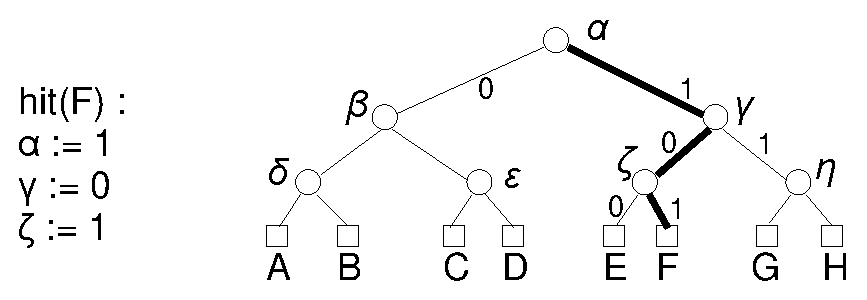
\includegraphics[width=0.7\textwidth]{2.theor/plruhit}\\
  \caption{Попадание для стратегия вытеснения \PseudoLRU
  (8-ассоциативная таблица)}\label{pseudo_lru_hit}
\end{figure}

На основании пометок вершин определяется и листовая вершина вытесняемой строки.
%Вытесняющий тег помещается в дереве на место вытесняемого.
Из корня дерева строится <<вытесняющий путь>> (он будет единственным), он приводит к вытесняемой строке. Начинает <<вытесняющий путь>> строиться из корневой вершины. Далее в <<вытесняющем пути>> исходящая дуга каждой вершины имеет пометку, противоположную пометке этой вершины. Т.е. если вершина помечена цифрой 0, значит дуга пути из этой вершины идет вправо, если вершина помечена цифрой 1 -- влево. Пример того, как определяется вытесняемая строка, показан на рис.~\ref{pseudo_lru_miss}. Цветом показаны пометки нелистовых вершин: черным
вершинам соответствует пометка 1, белым -- 0. В изображенном на рисунке дереве в качестве вытесняемой строки будет выбрана строка D, к которой ведет путь $\alpha-\beta-\varepsilon$.

\begin{figure}[h] \center
  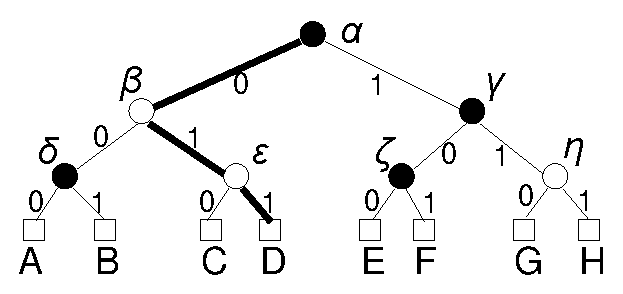
\includegraphics[width=0.5\textwidth]{2.theor/plrumiss}\\
  \caption{Определение вытесняемого элемента для стратегия вытеснения
  \PseudoLRU (8-ассоциативная таблица)}\label{pseudo_lru_miss}
\end{figure}


\subsubsection{Каноническое определение \PseudoLRU на битовой строке}

Для каждого региона хранится битовая строка $\beta$ длины $w{-}1$, где $w$ --
ассоциативность таблицы. Стратегия вытеснения определяется как процесс изменения
бит этой битовой строки.

Во многих книгах приводятся следующее определение стратегии
вытеснения \PseudoLRU для случая
$w=4$~\cite{FundamentalOfComputerOrganizationAndDesign} (в этом
случае для каждого региона выделяется 3 бита $B_1$, $B_2$ и $B_3$):
$$ \left[
  \begin{array}{c|ccc}
          & B_1 & B_2 & B_3 \\ \hline
    \pi_0 & 0 & 0 & \textsf{X} \\
    \pi_1 & 0 & 1 & \textsf{X} \\
    \pi_2 & 1 & \textsf{X} & 0 \\
    \pi_3 & 1 & \textsf{X} & 1 \\
  \end{array}
\right]
$$

Строки в регионе пронумерованы числами от 0 до $w{-}1$. При попадании на строку
региона с номером $i$ задействована строка матрицы, начинающаяся с $\pi_i$. Биты
$\beta$, напротив которых в строке матрицы находится \textsf{X}, не меняются.
Биты $\beta$, напротив которых в $i$'й строке находится число, принимают
значение, равное этому числу.

При промахе надо определить номер вытесняемой строки. Для этого используется
инвертированная форма той же матрицы (если элемент исходной матрицы был равен 0, то в инвертированной он равен 1; если в исходной равен 1, то в инвертированной равен 0; если в исходной равен \textsf{X}, то в инвертированной равен \textsf{X}):
$$
\left[
  \begin{array}{ccc|c}
    B_1 & B_2 & B_3 & \\ \hline
    1 & 1 & \textsf{X} & \rightarrow \pi_0 \\
    1 & 0 & \textsf{X} & \rightarrow \pi_1 \\
    0 & \textsf{X} & 1 & \rightarrow \pi_2 \\
    0 & \textsf{X} & 0 & \rightarrow \pi_3 \\
  \end{array}
\right]
$$

Выбирается строка матрицы, соответствующая текущему состоянию бит $B_1$,
$B_2$ и $B_3$, следующим образом: если напротив бита в строке матрицы находится число, бит
должен быть равен этому числу -- если напротив бита в строке матрицы
находится \textsf{X}, то соответствующий бит может иметь любое значение. Для любого набора значений $(B_1~B_2~B_3)$ подходящая строка матрицы всегда будет существовать и она будет единственной. Эта строка матрицы определяет вытесняемую строку региона.

Изменение $\beta$ обычно демонстрируют на бинарном дереве. Это то же дерево, что и в каноническом определении \PseudoLRU <<на бинарном дереве>>. $\beta$ составляется из пометок вершин дерева, начиная с корня и далее по слоям от левых к правым вершинам <<обходом в ширину>> (см. рис.~\ref{plru_bittree}).

\begin{figure}[h] \center
  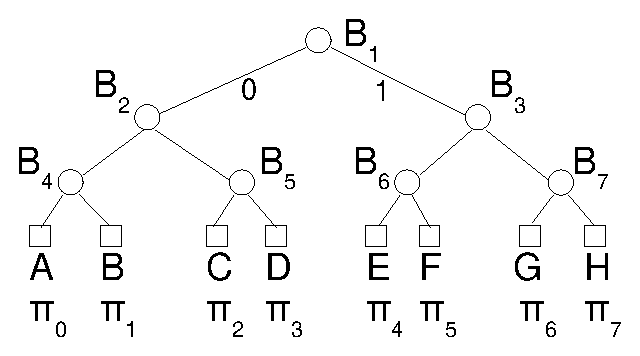
\includegraphics[width=0.5\textwidth]{2.theor/plru}\\
  \caption{Битовая строка в бинарном дереве}\label{plru_bittree}
\end{figure}

Формализованное описание для всех допустимых $w$ в литературе не
приводится. Однако в дальнейшем для формулирования и доказательства
утверждений про стратегию вытеснения \PseudoLRU такое описание будет
необходимо. Для $w=8$ изменение битовой строки будет задаваться следующей матрицей:
$$
\left[
  \begin{array}{c|ccccccc}
          & B_1 & B_2 & B_3 & B_4 & B_5 & B_6 & B_7 \\ \hline
    \pi_0 & 0 & 0 & \textsf{X} & 0 & \textsf{X} & \textsf{X} & \textsf{X} \\
    \pi_1 & 0 & 0 & \textsf{X} & 1 & \textsf{X} & \textsf{X} & \textsf{X} \\
    \pi_2 & 0 & 1 & \textsf{X} & \textsf{X} & 0 & \textsf{X} & \textsf{X} \\
    \pi_3 & 0 & 1 & \textsf{X} & \textsf{X} & 1 & \textsf{X} & \textsf{X} \\
    \pi_4 & 1 & \textsf{X} & 0 & \textsf{X} & \textsf{X} & 0 & \textsf{X} \\
    \pi_5 & 1 & \textsf{X} & 0 & \textsf{X} & \textsf{X} & 1 & \textsf{X} \\
    \pi_6 & 1 & \textsf{X} & 1 & \textsf{X} & \textsf{X} & \textsf{X} & 0 \\
    \pi_7 & 1 & \textsf{X} & 1 & \textsf{X} & \textsf{X} & \textsf{X} & 1 \\
  \end{array}
\right]
$$

Следующее утверждение~\ref{wMinus1PseudoLRU} дает алгоритм
преобразования битовой строки\\ $B_1,~B_2,~...,~B_{w{-}1}$ в результате
обращения в таблицу. В его формулировке будет применяться двоичное
разложение целых неотрицательных чисел от старших бит к младшим. Оно будет обозначаться для целого неотрицательного $x$ как $(x_1~x_2~...~x_n)_2$, где $x_i \in \{0, 1\}$ для $i = 1, 2, ..., n$, такие, что $x = x_n + 2{\cdot}x_{n-1} + 4{\cdot}x_{n-2} + \dots + 2^{n-1}{\cdot}x_1$. Например, 1 = (0 0 1)$_2$, 6 = (1 1 0)$_2$.

Обозначим символом $W$ выражение $\log_2 w$. По определению
стратегии вытеснения \PseudoLRU $W$ будет натуральным числом.

\begin{utv}[$(w{-}1)$-представление стратегии вытеснения
\PseudoLRU]\label{wMinus1PseudoLRU}При попадании по строке региона с номером $i = (i_1~i_2~\dots~i_W)_2$ происходит следующее изменение битовой строки $B_1,
B_2, ..., B_{w{-}1}$:

\parbox{0.3\textwidth}{
  $$ \begin{array}{l}
  B_{k_1} := i_1 \\
  B_{k_2} := i_2 \\
  B_{k_3} := i_3 \\
  ...\\
  B_{k_W} := i_W \\
  \end{array}$$
} \vline
\parbox{0.7\textwidth}{
  $$ \begin{array}{l}
  k_1 = (1)_2 \\
  k_2 = (1~i_1)_2 \\
  k_3 = (1~i_1~i_2)_2 \\
  ...\\
  k_W = (1~i_1~i_2~\dots~i_{W{-}1})_2 \\
  \end{array} $$
}
\\[1cm]

При промахе номер вытесняемой строки региона $j = (j_1~j_2~\dots~j_W)_2$ определяется следующим образом:

\parbox{0.3\textwidth}{
  $$ \begin{array}{l}
  i_1 = \neg B_{k_1} \\
  i_2 = \neg B_{k_2} \\
  i_3 = \neg B_{k_3} \\
  ...\\
  i_W = \neg B_{k_W} \\
  \end{array}$$
} \vline
\parbox{0.7\textwidth}{
  $$ \begin{array}{l}
  k_1 = (1)_2 \\
  k_2 = (1~\neg B_{k_1})_2 \\
  k_3 = (1~\neg B_{k_1}~\neg B_{k_2})_2 \\
  ...\\
  k_W = (1~\neg B_{k_1}~\neg B_{k_2}\dots\neg B_{k_{W{-}1}})_2 \\
  \end{array} $$
}
\\[0.5cm]

Кроме того при промахе делается такое же преобразование бит $B_1$, $B_2$, ..., $B_{w{-}1}$, как и в случае попадания на строку с номером $j$.
\end{utv}

Прямой проверкой нетрудно убедиться, что это утверждение верно для $w$ = 4 и 8.

\subsubsection{Определение \PseudoLRU на ветвях бинарного
дерева}\label{sec:PseudoLRUonBranches}

Здесь будет показано, как из канонических определений \PseudoLRU
получить формулировку \PseudoLRU с точки зрения одной строки региона~\cite{my_lomonosov_2010}
(в канонических определениях рассматривается весь регион целиком и
для него формулируются правила работы с последовательностью бит $B_1,
B_2, ..., B_{w{-}1}$ или пометками вершин бинарного дерева). Описываемое в этом разделе определение \PseudoLRU ранее не встречалось в литературе.

Сначала этот переход покажем в частном случае, на примере $w=4$. Первый шаг --- это
смена <<состояния>>: вместо последовательности бит $B_1, B_2, ...,
B_{w-1}$ будем рассматривать последовательность векторов бит
$\beta_0,~\beta_1,~\dots,~\beta_{w-1}$, каждый $\beta_i$ --- это вектор из $W$ бит. Каждый $\beta_i$ соответствует $i$'й листовой вершине бинарного дерева (см. рисунок~\ref{fig:plru_def_step1}). Попадание
меняет теперь атрибуты не внутренних вершин дерева $(B_1~B_2~B_3)$, а листовых $(\beta_0~...~\beta_3)$.
Каждый $\beta_i$ будет представляться списком длины $W$, обозначающим путь от
корня дерева к $i$'й листовой вершине: $\beta_0$ соответствует
($B_1$ $B_2$), $\beta_1$ соответствует ($B_1$ $\neg B_2$), $\beta_2$
соответствует ($\neg B_1$ $B_3$) и $\beta_3$ соответствует ($\neg
B_1$ $ \neg B_3$).\\[0.5cm]

\begin{figure}[h]
\parbox{0.2\textwidth}{ \centering
  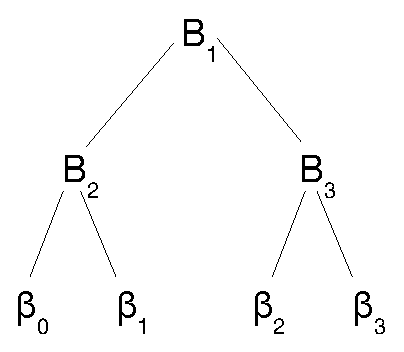
\includegraphics[width=0.2\textwidth]{1.review/btree}
}
\parbox{0.25\textwidth}{
$$ \left[
  \begin{array}{c|ccc}
          & B_1 & B_2 & B_3 \\ \hline
    \pi_0 & 0 & 0 & \textsf{X} \\
    \pi_1 & 0 & 1 & \textsf{X} \\
    \pi_2 & 1 & \textsf{X} & 0 \\
    \pi_3 & 1 & \textsf{X} & 1 \\
  \end{array}
\right]
$$
} $\stackrel{1}{\longrightarrow}$ %\vline
\parbox{0.4\textwidth}{
$$ \left[
  \begin{array}{c|cccc}
          & \beta_0 & \beta_1 & \beta_2 & \beta_3 \\ \hline
    \pi_0 & (0~0) & (0~1) & (1~\textsf{X}) & (1~\textsf{X}) \\
    \pi_1 & (0~1) & (0~0) & (1~\textsf{X}) & (1~\textsf{X}) \\
    \pi_2 & (1~\textsf{X}) & (1~\textsf{X}) & (0~0) & (0~1) \\
    \pi_3 & (1~\textsf{X}) & (1~\textsf{X}) & (0~1) & (0~0) \\
  \end{array}
\right]
$$
}
\caption{Смена состояния}\label{fig:plru_def_step1}
\end{figure}

Заметим, что получилась симметричная матрица. На пересечении $\pi_i$
и $\beta_j$ располагается вектор, задающий изменение $\beta_j$ (вектора в $j$'й
листовой вершине дерева) при попадании по строке региона, соответствующей $i$'й листовой вершине дерева. Назовем позицию $i \oplus j$ \emph{относительной позицией}
$i$ относительно $j$. Рассмотрим отдельно каждый столбец
получившейся матрицы (на рисунке~\ref{fig:plru_def_step2} до стрелки) и упорядочим строки столбцов в порядке увеличения относительных позиций (на рисунке~\ref{fig:plru_def_step2} после стрелки).

\begin{figure}[h]
\parbox{0.2\textwidth}{
$$ \left[
  \begin{array}{c|c}
          & \beta_0 \\ \hline
    \pi_0 & (0~0) \\
    \pi_1 & (0~1) \\
    \pi_2 & (1~\textsf{X}) \\
    \pi_3 & (1~\textsf{X}) \\
  \end{array}
\right]
$$
}\parbox{0.2\textwidth}{
$$ \left[
  \begin{array}{c|c}
          & \beta_1 \\ \hline
    \pi_0 & (0~1) \\
    \pi_1 & (0~0) \\
    \pi_2 & (1~\textsf{X}) \\
    \pi_3 & (1~\textsf{X}) \\
  \end{array}
\right]
$$
}\parbox{0.2\textwidth}{
$$ \left[
  \begin{array}{c|c}
          & \beta_2 \\ \hline
    \pi_0 & (1~\textsf{X}) \\
    \pi_1 & (1~\textsf{X}) \\
    \pi_2 & (0~0) \\
    \pi_3 & (0~1) \\
  \end{array}
\right]
$$
}\parbox{0.2\textwidth}{
$$ \left[
  \begin{array}{c|c}
          & \beta_3 \\ \hline
    \pi_0 & (1~\textsf{X}) \\
    \pi_1 & (1~\textsf{X}) \\
    \pi_2 & (0~1) \\
    \pi_3 & (0~0) \\
  \end{array}
\right]
$$
} $\stackrel{2}{\stackrel{\longrightarrow}{\pi^i_j \equiv \pi_{i
\oplus j}}}$

\parbox{0.24\textwidth}{
$$ \left[
  \begin{array}{c|c}
          & \beta_0 \\ \hline
    \pi^0_0 \equiv \pi_0 & (0~0) \\
    \pi^0_1 \equiv \pi_1 & (0~1) \\
    \pi^0_2 \equiv \pi_2 & (1~\textsf{X}) \\
    \pi^0_3 \equiv \pi_3 & (1~\textsf{X}) \\
  \end{array}
\right]
$$
}\parbox{0.24\textwidth}{
$$ \left[
  \begin{array}{c|c}
          & \beta_1 \\ \hline
    \pi^1_0 \equiv \pi_1 & (0~0) \\
    \pi^1_1 \equiv \pi_0 & (0~1) \\
    \pi^1_2 \equiv \pi_3 & (1~\textsf{X}) \\
    \pi^1_3 \equiv \pi_2 & (1~\textsf{X}) \\
  \end{array}
\right]
$$
}\parbox{0.24\textwidth}{
$$ \left[
  \begin{array}{c|c}
          & \beta_2 \\ \hline
    \pi^2_0 \equiv \pi_2 & (0~0) \\
    \pi^2_1 \equiv \pi_3 & (0~1) \\
    \pi^2_2 \equiv \pi_0 & (1~\textsf{X}) \\
    \pi^2_3 \equiv \pi_1 & (1~\textsf{X}) \\
  \end{array}
\right]
$$
}\parbox{0.24\textwidth}{
$$ \left[
  \begin{array}{c|c}
          & \beta_3 \\ \hline
    \pi^3_0 \equiv \pi_3 & (0~0) \\
    \pi^3_1 \equiv \pi_2 & (0~1) \\
    \pi^3_2 \equiv \pi_1 & (1~\textsf{X}) \\
    \pi^3_3 \equiv \pi_0 & (1~\textsf{X}) \\
  \end{array}
\right]
$$
}
\caption{Нумерация относительными позициями}\label{fig:plru_def_step2}
\end{figure}

После перехода к относительным позициям ($\pi^i_j$ -- это позиция
$\pi_j$ относительно $\pi_i$, т.е. $\pi_{i \oplus j}$) все столбцы получились одинаковыми.
Иными словами, \emph{алгоритм изменения порядка строк региона согласно стратегии
вытеснения \PseudoLRU на относительных позициях инвариантен
относительно абсолютной позиции вытесняемой строки}. Следующая теорема
формально доказывает этот факт.

Будем называть \emph{\PseudoLRU-ветвью позиции $i$} вектор
$(B_{k_1}^{\sigma_1}~B_{k_2}^{\sigma_2}~\dots~B_{k_W}^{\sigma_W})$,
в котором $k_1 = (1)_2, \sigma_1 = \neg i_1, \sigma_j = \neg i_j$, $k_j = (1~i_1~i_2~\dots~i_{j-1})_2$, $j = 2, 3, \dots, W$, $i = (i_1~i_2~\dots~i_W)_2$. Степени определены стандартным образом: $B^1 \equiv B, B^0 \equiv \neg B$. Например, \PseudoLRU-ветвью позиции 0 есть $(B_1~B_2~B_4~...)$. Каждой строке региона (т.е. каждой позиции строк региона) соответствует своя \PseudoLRU-ветвь. Каждое обращение изменяет все ветви некоторым образом, который не зависит от абсолютной позиции, а зависит от относительной:

\begin{theorem}[Инвариантность преобразования \PseudoLRU-ветвей относительными
позициями]\label{thm_pseudoLRU_invariant} \PseudoLRUInvariant
\end{theorem}
Доказательство теоремы приведено в приложении~\ref{sec:proofs}.

Доказанный факт позволяет сформулировать определение стратегии
вытеснения \PseudoLRU, сфокусированное не на изменении атрибутов строк всего
региона,
а на изменении атрибутов одной строки. На этом определении
будут базироваться применения предлагаемых методов генерации
ограничений для стратегии вытеснения \PseudoLRU.

\begin{utv}[формулировка \PseudoLRU на ветвях бинарного дерева]
Сопоставим некоторой произвольной строке региона вектор длины $W$. Каждое обращение к этой строке региона делает её вектор равным (0 0 ... 0). Строка региона является вытесняемой, если её вектор равен (1 1 ... 1).
Влияние других обращений определяется относительной позицией их
строки региона относительно позиции данной строки региона. Если относительная позиция
принадлежит области $[\frac{w}{2^k},~\frac{w}{2^{k-1}}), k =
1,2,...,W$, то первые $k{-}1$ элементов битового вектора становятся равными
0, $k$'й элемент вектора становится равным 1, остальные элементы
вектора не меняются. Если относительная позиция равна 0, то все элементы вектора становятся равными 0.
\end{utv}

Битовый вектор длины $W$ будет соответствовать пути из корня бинарного
дерева в листовую вершину, соответствующую данной строке региона.
Удобно представлять процесс изменения элементов бинарного вектора  в виде их
\emph{перекрашивания}. Про элементы битового вектора, равные 0,
будем говорить, что они покрашены в \emph{белый} цвет, а элементы вектора, равные 1, --- в\emph{черный}.

Говоря в терминах бинарного дерева из канонических определений \PseudoLRU, каждое обращение в регион изменяет пометки в нелистовых вершинах дерева. Каждой листовой вершине соответствует единственный в нее путь из корня дерева (та самая <<ветвь>>). Вершина дерева, входящая в ветвь, с точки зрения этой ветви будет <<белой>>, если пометка этой вершины совпадает с направлением дуги дерева из этой вершины. входящей в ветвь, <<черной>> --- если не совпадает. Вытесняется та строка региона, путь к которой полностью состоит из несоответствующих дуг по каноническим определениям, т.е. из черных вершин по новому определению. На рисунке~\ref{recolor}
изображен процесс перекрашивания ветви, ведущей в А, под действием
попадания в C (для сокращения показана только ветвь в А без
остальной части дерева). Так как путь из корня в C совпадает из
верхних двух вершин, то они перекрашиваются в белый цвет. Дуга из
третьей вершины пути в С не совпадает с дугой пути в А, поэтому
третья вершина перекрашивается в черный цвет. Остальные вершины
ветви остаются без изменений.

\begin{figure}[h] \center
  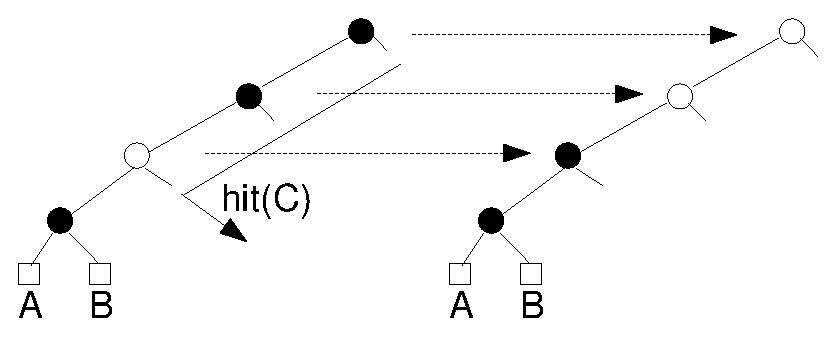
\includegraphics[width=0.8\textwidth]{1.review/recolor}\\
  \caption{Перекрашивание ветви в А}\label{recolor}
\end{figure}


Определение стратегии вытеснения \PseudoLRU на ветвях дерева
является связующим звеном между каноническим определением (например,
на битовой строке) и определением с помощью таблицы вытеснения,
поскольку ветвь -- это и есть двоичное разложение позиции, которая меняется точно так же, как и позиция в перестановке согласно таблице вытеснения.


%%%%%%%%%%%%%%%%%%%%%%%%%%%%%%%%%%%%%%%%%%%%%%%%%%%%%%%%%%%%%%%%%%%%

\section{Метод полезных обращений для записи стратегии вытеснения в виде ограничений}\label{sec:usefulness_functions}

%{\footnotesize В разделе рассматривается метод составления ограничений для
%описания стратегии вытеснения, для которой удается определить функционал
%вытеснения. Стратегия вытеснения описывается ограничением сверху на количество \emph{полезных} инструкций (т.е. помогающих вытеснению).
%В разделе приведены определения полезных инструкций и способы составления ограничений для трех
%наиболее часто используемых в микропроцессорах стратегий вытеснения -- \LRU, \FIFO и \PseudoLRU. Освещается понятие \emph{монотонного функционала вытеснения}, который является залогом более
%простой системы ограничений.}

В данном разделе процесс вытеснения будет представляться как изменение  системы функций, отображающих ключи в целые числа. Каждое обращение в таблицу изменяет значения функций по всем ключам\footnote{это напоминает изменение операций в рамках машин абстрактного состояния Ю.Гуревича~\cite{ASM}}. Пример процесса изменения значения функции для некоторого ключа изображен на рисунке~\ref{fig:graphic}.

\begin{figure}[h] \center
  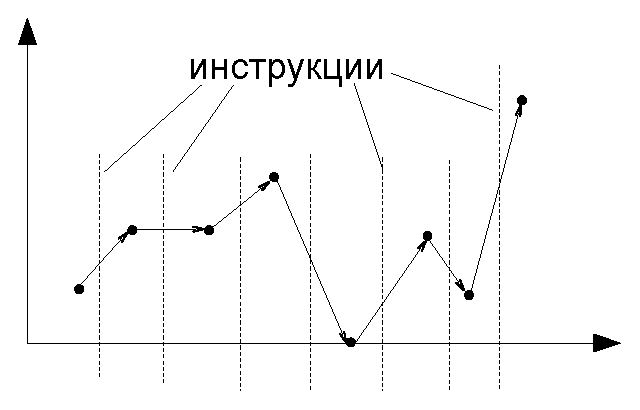
\includegraphics[width=0.7\textwidth]{2.theor/graphic}\\
  \caption{К определению стратегии вытеснения}\label{fig:graphic}
\end{figure}

Говоря формально, пусть $\alpha, \beta, \dots, \gamma$ --- одноместные функции,
отображающие ключи в целые числа. Для каждого обращения определены функции
изменения значений функций $\alpha, \beta, \dots, \gamma$ (если не сказано иное, будет предполагаться, что обращения осуществляются в один и тот же регион):
$$\parbox{2.5cm}{in-parallel\\forall keys x~}\left|\begin{array}{l}
\alpha(x) := A_I(k, \alpha, \beta, \dots, \gamma)\\
\beta(x) := B_I(k, \alpha, \beta, \dots, \gamma)\\
\dots\\
\gamma(x) := C_I(k, \alpha, \beta, \dots, \gamma)\\
\end{array}\right.
$$

Обновления значений функций $\alpha, \beta, \dots, \gamma$ выполняются одновременно. $I$ --- обращение в таблицу, $k$ --- ключ в этом обращении. Функции $A_I$, $B_I$, \dots, $C_I$ отражают влияние обращения по некоторому ключу на другой произвольный ключ. $x$ --- это ключ, за которым <<следим>> и условия вытеснения которого нас интересуют, а $k$ ---это ключ в очередном обращении из тестового шаблона.
Возможны следующие случаи (в качестве $x$ рассматривается произвольный ключ, не
обязательно <<находящийся>> в регионе):
\begin{itemize}
    \item в результате обращения по ключу $k$ ключ $x$ <<попадает>> в регион (т.е. в регион добавляется строка с ключом $x$);
    \item в результате обращения по ключу $k$ ключ $x$ <<вытесняется>> из региона (т.е. из региона удаляется строка с ключом $x$);
    \item в результате обращения по ключу $k$ <<состояние>> ключа $x$ в регионе не меняется.
\end{itemize}

%Этим ситуациям как раз и ставятся в соответствие классы значений функций $\alpha, \beta, \dots, \gamma$, а функции $A_I$, $B_I$, \dots, $C_I$ осуществляют переход между этими классами. Тем самым стратегия вытеснения будет описана в виде изменения таких <<счетчиков>> $\alpha, \beta, \dots, \gamma$.

%Формально это правило выражается следующим образом.
Будем называть функцию
$\alpha$, отображающую ключи в целые числа, \emph{функционалом вытеснения} для заданной стратегии вытеснения, если одновременно выполнены следующие свойства:
\begin{enumerate}
  \item существуют константы $\alpha_{min}$ и $\alpha_{max}$ такие, что
$\alpha_{min} \leqslant \alpha_{max}$;
  \item для любого ключа $x$ $\alpha_{min} \leqslant \alpha(x) \leqslant
\alpha_{max}$ тогда и только тогда, когда $x$ находится в регионе по определению
стратегии вытеснения (т.е. <<был помещен>> в регион и до сих пор не вытеснен);
  \item для любого ключа $k$ $A_I(k, \alpha,\beta,\dots,\gamma) (k) =
\alpha_{min}$;
  \item $\exists! \varphi: \mbox{~ключ~} \times \mathds{Z}^{n} \times \mbox{~ключ~} \times \mathds{Z}^{n} \rightarrow
\mathds{Z}$, где $n$ --- количество функций во множестве
$\{\alpha,\beta,\dots,\gamma\}$, такая, что для любого ключа $x$ $$A_I(k,
\alpha,\beta,\dots,\gamma)(x) \equiv \varphi(k, \alpha(k), \beta(k), \dots,
\gamma(k), x, \alpha(x), \beta(x), \dots, \gamma(x))$$ иными словами, в функции
изменения функционала вытеснения разрешается обращаться только к $k$ и тому ключу,
для которого определяется функционал вытеснения;
  \item $\exists!$ ключ $x^* : \alpha(x^*) = \alpha_{max}$;
  \item перед любым неуспешным обращением $\alpha(x^*) =
\alpha_{max}$ тогда и только тогда, когда $x^*$ есть <<вытесняемый>> ключ по
определению стратегии вытеснения (т.е. строка с ключом $x^*$ является
вытесняемой при данном обращении по определению стратегии вытеснения);
\end{enumerate}

Пример функционала вытеснения: $\alpha$ --- счетчик количества обращений к строке
для стратегии вытеснения \LRU. Обращение по тому же ключу делает $\alpha$
равным 1, по другому ключу --- увеличивает $\alpha$ на единицу. Вытесняемым
считается ключ, чей счетчик равен $w$ --- количеству строк в регионе. Проверим
определение функционала вытеснения:
\begin{enumerate}
    \item $\alpha_{min}$ = 1, $\alpha_{max}$ = $w$, $1 \leqslant w$;
    \item верно, что счетчик больше $w$ тогда и только тогда, когда $x$ не
находится в регионе; в противном случае, было бы возможно подряд успешно обратиться к
большему числу строк, чем хранится в регионе;
    \item по условию обращение по тому же ключу делает $\alpha$ равным 1, что
и есть $A_I(x;...)(x) = 1$;
    \item изменение одного счетчика производится независимо от изменений других счетчиков (хотя, конечно, все счетчики изменяются одновременно);
    \item такой $x^*$ существует, ибо в противном случае было бы возможно подряд успешно обратиться к большему числу строк, чем хранится в регионе; такой $x^*$ единственный, поскольку каждое обращение меняет каждый счетчик и в минимальное значение $\alpha$ изменяется лишь по единственному ключу.
\end{enumerate}

Пусть для стратегии вытеснения сформулирован функционал вытеснения. Будем называть
обращение по некоторому ключу \emph{полезным для вытеснения} ключа
$x$ (или просто, \emph{полезным}), если оно монотонно увеличивает функционал вытеснения по
ключу $x$ до максимального значения (см. рис.~\ref{useful}).\\

\begin{figure}[h] \center
  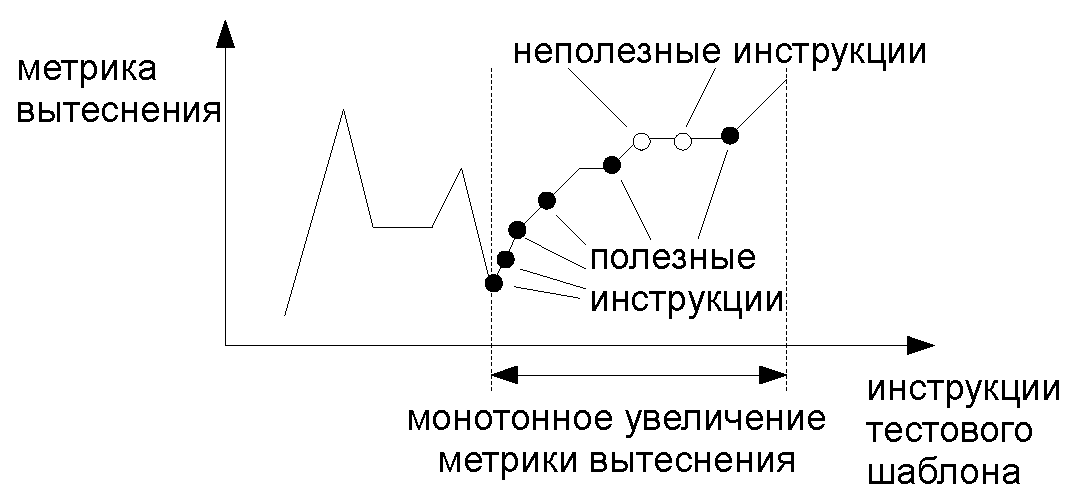
\includegraphics[width=0.6\textwidth]{2.theor/useful}\\
  \caption{К определению полезных обращений}\label{useful}
\end{figure}

Тогда вытеснение будет происходить в том случае, когда количество
полезных обращений превысит некоторое константное количество.
И вытеснение не будет происходить, если это количество не превысит некоторой константной верхней границы.

\emph{Формулой полезного обращения} будем называть предикат от вытесняемого ключа $k$ и региона $R$ и ключей и регионов предыдущих обращений, при которых это обращение будет полезным для вытеснения ключа $k$ из региона $R$.

Тем самым ограничение (constraint) <<быть вытесненным>> представимо в виде
ограничения сверху на <<сумму>> формул полезных обращений по всем предыдущим обращениям: $\sum_{i=1}^n [u_x(k_i)] < N$, где $u_x(k_i)$ -- формула полезного обращения по ключу $k_i$ для ключа $x$ в полностью ассоциативной таблице, для остальных таблиц будут указываться регионы обращений: $u_{x,r}(k_i, r_i)$.

Формулы полезных обращений, как и функционалы вытеснения, не являются единственными. Например, для стратегии вытеснения \LRU возможны следующие две различные формулы полезных обращений (далее для одной из них будет формально показано, что она действительно задает полезные обращения) (формулы приведены для случая полностью ассоциативной таблицы):
\begin{itemize}
  \item $u_x(x_i) \equiv (x \notin \{x_i, x_{i+1}, ..., x_n\} \wedge
\bigwedge\limits_{j=1}^{i-1} (x \in \{x_j, x_{j+1}, ..., x_{i-1}\} \vee x_j
\neq x_i))$ -- обращение считается полезным, если оно расположена после
последнего обращения к $x$ и с того момента является первым обращением к своему
ключу; нетрудно заметить, что это в чистом виде определение \LRU, изображенное на рисунке~\ref{fig:lru1}: обращение по ключу $x_j$, который расположен после ключа $x$, передвигает $x$ к концу вектора, за концом происходит вытеснение; первые обращения по ключам после последнего обращения к $x$ -- это и есть именно те обращения, где $x$ сдвигается к концу; иначе говоря, полезное обращение сдвигает $x$ к концу, приближая его к вытеснению;
  \item $u_x(x_i) \equiv (x \notin \{x_i, x_{i+1}, ..., x_n\} \wedge x_i \notin
\{x_{i+1}, x_{i+2}, ..., x_n\})$ -- обращение считается полезным, если оно
расположено после последнего обращения к $x$ и является последним обращением к
своему ключу перед финальным обращением к $x$; т.е. в таблице хранятся некоторые ключи, есть некоторый ключ $x$, есть последовательность других обращений (их
ключи обозначены как  $x_i$, ..., $x_n$), полезными будут лишь последние к ним обращения (среди $x_i$, ..., $x_n$ могут быть равные), т.е. все полезные обращения вместе образуют (по разу) все различные ключи.
\end{itemize}

Тем самым, метод полезных обращений состоит в следующем:
\begin{enumerate}
  \item выделить функционал вытеснения $\alpha$;
  \item выделить определение полезной инструкции;
  \item записать формулу полезного обращения $u_{x,r}(x_i, r_i)$ для обращения с ключом $x$ и регионом $r$;
  \item определить $\alpha_{max}$;
  \item составить ограничение для свойства <<$x$ вытеснен>> в виде
$\sum\limits_{i=1}^n u_{x,r}(x_i, r_i) > \alpha_{max}$ и для свойства <<$x$ не
вытеснен>> в виде $\sum\limits_{i=1}^n u_{x,r}(x_i,r_i) \leqslant \alpha_{max}$.
\end{enumerate}

Ключевой вопрос при применении метода полезных обращений --- это выбор
функционала вытеснения. От него в том числе будет зависеть сложность функции
полезности и генерируемых ограничений.

 Функционал вытеснения может быть получен из таблицы вытеснения
(policy table). А именно, если вытеснение происходит с позиции с максимальным
номером (т.е. в последней строке отсутствует число $w{-}1$), а в результате
попадания ключ переносится в самое начало (т.е. второй столбец имеет вид (0 1 2
... $w{-}1$ $m$)$^T$ ). Тогда $\alpha$ --- это позиция ключа в перестановке,
$\alpha_{min}$ = 0, $\alpha_{max} = w{-}1$. Этими свойствами, например, обладают
таблицы вытеснения \LRU (см.рис.~\ref{fig:PolicyTableLRU8}) и
\PseudoLRU~\cite{policy_tables}.

%В отличие от метода диапазонов вытеснения при использовании функций полезности не происходит выделение участка тестового шаблона, непосредственно влияющего на вытеснение. Считается, что это влияние начинается с момента появления строки в таблице. Другое дело, что одни инструкции влияют на ее вытеснение (это и есть <<полезные>> инструкции), а другие -- нет.


\subsection{Метод полезных обращений для стратегии вытеснения \LRU}

\LRU (Least Recently Used) --- это стратегия вытеснения,
определяющая вытесняемые данные как наименее используемые. Она
эффективна для алгоритмов, обладающих свойством локальности данных,
т.е. чаще использующих те данные, к которым недавно происходило
обращение. Эта стратегия используется, например, в микропроцессорах
архитектуры MIPS~\cite{mips64II}.

Стратегия вытеснения \LRU обычно определяется с использованием
счетчиков обращений. Для каждой строки таблицы
вводится счетчик обращений к ней. Каждое обращение увеличивает
счетчик. Счетчик вытесняющей строки на единицу больше максимального счетчика невытесняемых строк. Вытесняемой в регионе будет строка с минимальным счетчиком его строк.
%Поскольку границы значений счетчика неизвестны, формулирование
%функционала вытеснения на основе счетчика провести сложно.

Другой способ описания \LRU основан на введении порядка на строках региона (т.е.
регион представляется вектором строк). После каждой инструкции элементы этого вектора переупорядочиваются, \emph{переставляются}, согласно следующим правилам (см.рис.~\ref{fig:lru1}):
\begin{itemize}
\item при попадании соответствующая строка перемещается в начало, строки, которые расположены левее этой, сдвигаются на одну позицию вправо;
\item при промахе вытесняется последняя строка, в начало вставляется вытесняющая.
\end{itemize}

\begin{figure}[h] \center
  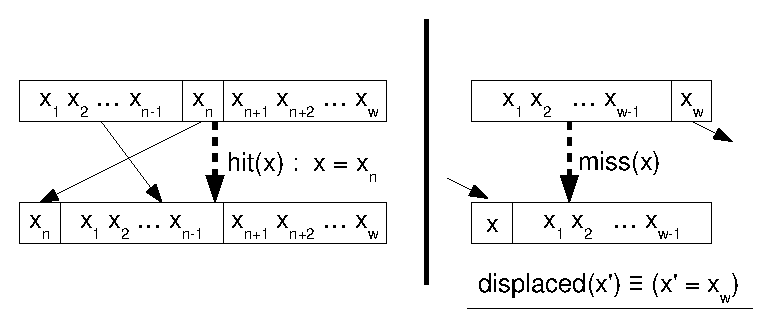
\includegraphics[width=0.6\textwidth]{2.theor/lru1}\\
  \caption{Стратегия вытеснения \LRU (w --- ассоциативность) на
перестановках}\label{fig:lru1}
\end{figure}

Позиция строки, ее индекс, в таком векторе ограничена, единственна, ее изменение допускает представление, независимое от других ключей. Тем самым \emph{<<позиция>> ключа является функционалом вытеснения}.

Функция изменения этого функционала выглядит следующим образом:\\

\parbox{0.5\textwidth}{ \tt
$A_{\mbox{hit}}(k, \alpha)(x) \equiv$\\
if $\alpha(x) > w$ then $\alpha(x)$\\
elsif $\alpha(k) > \alpha(x)$ then $\alpha(x)+1$\\
elsif $\alpha(k) = \alpha(x)$ then $1$\\
else $\alpha(x)$ endif%
}\parbox{0.5\textwidth}{\tt
$A_{\mbox{miss}}(k, \alpha)(x) \equiv$\\
if $k = x$ then $1$\\
elsif $\alpha(x) > w$ then $\alpha(x)$\\
else $\alpha(x) + 1$ endif}\\

Полезным будет считаться обращение, увеличивающее позицию, т.е.
переставляющее соответствующий ключ к концу. Такими обращениями являются все
промахи (поскольку они вытесняют последнюю строку вектора с передвижением всех остальных на одну позицию к концу, т.е. будет передвинута и строка с ключом $x$) и
попадания к строкам, находившимся ближе к концу, чем $x$ (потому как при попадании они передвинутся в самое начало, а все строки от начала и до них сдвинутся на одну
позицию к концу, в том числе и $x$).

Осталось выразить эту идею в виде ограничений~\cite{my_ewdts_2009}.
Учет полезных обращений начинается уже в инициализирующей последовательности,
тем самым необходимо будет сформулировать формулы полезных обращений и для
инициализирующих обращений.

Следующая теорема описывает функцию полезности для \LRU ($m$ --- количество
инициализирующих инструкций):

\begin{theorem}[Выражение свойства <<быть вытесненным>> для \LRU]\label{correct_mirror_LRU} \LRUusefuls
\end{theorem}

\begin{proof}
По определению стратегии вытеснения \LRU <<$k$ не вытеснен из региона $R$ согласно определению на перестановках>> эквивалентно тому, что после последнего обращения к $k$ в $R$ происходит не более $w$ обращений по различным ключам в регион $R$. Несложно убедиться, что это количество выражается следующей формулой: $$|\{s_i| R = R(s_i) \wedge s \notin \{s_i, ..., s_{m+n}\}\}|$$
Однако это же число можно записать другим образом, чтобы исключить повторения одинаковых $s_i$:
$$|\{s_i| R = R(s_i) \wedge s \notin \{s_i, ..., s_{m+n}\} \wedge s_i \notin \{s_{i+1}, ..., s_{m+n}\}\}|$$

Ввиду конечности последовательности $\langle s_i, ..., s_{m+n}\rangle$ в нем всегда найдется последнее вхождение $s_i$ --- множество последних вхождений всех элементов списка равно множеству всех элементов списка.

Представленная мощность множества и есть требуемая сумма.
\end{proof}

Из теоремы~\ref{correct_mirror_LRU} следует система ограничений для
описания обращений по ключу $k_i$ в регион $R_i$ согласно методу полезных обращений для \LRU: \begin{itemize}
\item для hit($k_i, R_i$):
$$
\left\{\begin{array}{l} (k_i||R_i) \in \{(t_1||r_1), ..., (t_m||r_m), (k_1||R_1),
..., (k_{i-1}||R_{i-1})\}\\
\sum\limits_{j=1}^m [u_{k_i,R_i}(t_j||r_j)] + \sum\limits_{j=1}^{i-1} [u_{k_i,R_i}(k_j||R_j)] < w\\
\{(t_1||r_1), ..., (t_m||r_m)\} - \mbox{все разные}\\
\end{array} \right.
$$
\item для miss($k_i, R_i$):
$$
\left\{\begin{array}{l} (k_i||R_i) \in \{(t_1||r_1), ..., (t_m||r_m), (k_1||R_1),
..., (k_{i-1}||R_{i-1})\}\\
\sum\limits_{i=1}^m [u_{k_i,R_i}(t_j||r_j)] + \sum\limits_{j=1}^{i-1} [u_{k_i,R_i}(k_j||R_j)]
\geqslant w\\
\{(t_1||r_1), ..., (t_m||r_m)\} - \mbox{все разные}\\
\end{array} \right.
$$
\end{itemize}


%Для этого удобно использовать утверждение~\ref{hit_miss_human}. Символом
%$\lambda_\delta$ будет обозначаться элемент начального
%состояния таблицы с индексом $\delta$ по порядку \LRU, $1 \leqslant \delta \leqslant w$. Индекс 1 обозначает самый молодой элемент, индекс $w$ обозначает самый старый элемент.
%
%Применение полезностей эффективно в том случае, когда домен имеет
%небольшой размер. В этом случае можно перебрать все элементы
%домена (это и будут $\lambda_\delta$) и составить для них свои
%полезности, причем для каждого элемента будет известен индекс по
%порядку \LRU ($\delta$). Ограничение, описывающее стратегию
%вытеснения, будет при этом иметь вид дизъюнкции по элементам домена.
%
%Если вытесняемый элемент был в начальном состоянии (пусть это
%$\lambda_\delta$) и к нему не было обращений, то для его вытеснения
%необходимо $w-\delta + 1$ полезных инструкций, потому что столько
%раз надо подвинуть элемент с индексом $\delta$ в \LRU-списке в
%сторону к концу (к элементам с индексом $w$), чтобы он вышел за
%границу списка (иными словами, чтобы он был вытеснен).
%
%Если вытесняемый элемент был в начальном состоянии и к нему было
%обращение, то для его вытеснения необходимо $w$ инструкций, так как
%во время обращения элемент был поставлен в самое начало \LRU-списка.
%То же справедливо для внесенных в кэширующий буфер новых тегсетов --
%чтобы их вытеснить, надо так же $w$ полезных инструкций, чтобы
%переместить их к концу \LRU-списка.
%
%В таблице~\ref{hit_miss_table} приведены все функции полезности для
%кэш-попаданий и кэш-промахов. Доказательство корректности приведенных
% в ней формул (т.е. доказательство того, что эти формулы действительно
% описывают \LRU) важны, но не представляют самостоятельного результата.
%Поэтому они были вынесены за пределы основной части диссертации и
%находятся в приложении~\ref{sec:proofs}.

В некоторых случаях количество ограничений удается сократить, используя следующую эвристику для ограничения вида $\sum_{i=1}^n a_i \leqslant C$:
\begin{itemize}
    \item если $C > n$, то его не включать в конъюнкцию;
    \item если $C < 0$, то вся конъюнкция с этим ограничением несовместна;
    \item если $C = 0$, то его сразу расписать в конъюнкцию ограничений
$a_i = 0$ для каждого $i$ от 1 до $n$;
    \item если $C = n$, то его сразу расписать в конъюнкцию ограничений
$a_i = 1$ для каждого $i$ от 1 до $n$.
\end{itemize}

Аналогично с ограничениями вида $\sum_{i=1}^n a_i \geqslant C$.


\subsection{Метод полезных обращений для стратегии вытеснения \FIFO}

\FIFO (First-In First-Out) -- это стратегия вытеснения, определяющая
вытесняемые данные согласно принципу очереди FIFO. Например, в
микропроцессоре PowerPC 970FX вытеснение из небольшого буфера,
хранящего последние преобразованные эффективные адреса в физические,
D-ERAT, происходит согласно \FIFO~\cite{PowerPC970FXUserManual}.

Стратегия \FIFO допускает описание на основе порядка на строках
региона (т.е. регион представляется вектором строк-элементов). После каждого
обращения строки вектора переупорядочиваются, \emph{перставляются}, согласно следующим правилам
(см.рис.~\ref{fifo1}):
\begin{itemize}
\item при попадании порядок строк не меняется;
\item при промахе вытесняется последняя строка, в начало вставляется вытесняющая строка.
\end{itemize}

\begin{figure}[h] \center
  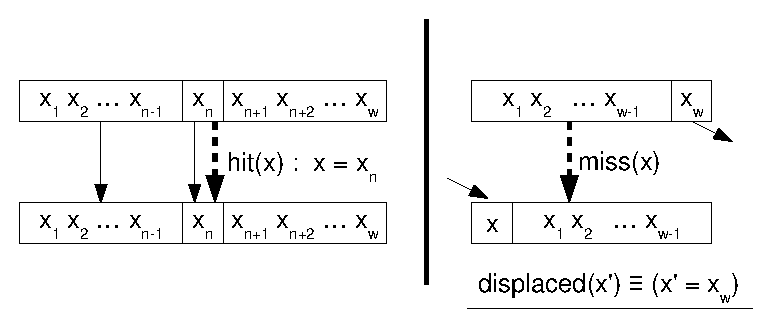
\includegraphics[width=0.6\textwidth]{2.theor/fifo1}\\
  \caption{Стратегия вытеснения \FIFO (w --- ассоциативность
таблицы)}\label{fifo1}
\end{figure}

Отличие от \LRU лишь в том, что при \FIFO не происходит перестановки
строк при возникновении попадания. Поэтому таблица
вытеснения~\cite{policy_tables} для стратегии вытеснения \FIFO будет
выглядеть так, как изображено на рисунке~\ref{fifo_policy_table}.

\begin{figure}[h]
$$
  \left[
    \begin{array}{c|cccccc}
      \pi_0 & 0 & 1 & 2 & 3 & \dots & w{-}1 \\
      \pi_1 & 0 & 1 & 2 & 3 & \dots & w{-}1 \\
      \pi_2 & 0 & 1 & 2 & 3 & \dots & w{-}1 \\
      \vdots &  &  &  & & & \\
      \pi_{w-1} & 0 & 1 & 2 & 3 & \dots & w{-}1 \\
      \pi_m & m & 0 & 1 & 2 & \dots & w{-}2 \\
    \end{array}
  \right]
$$
\caption{Таблица вытеснения для \FIFO}\label{fifo_policy_table}
\end{figure}

Формулы полезных обращений для \FIFO будем строить также на основе уже сформулированных и обоснованных формул для \LRU.

%Кроме того все инструкции с попаданиями, поскольку они не влияют на вытеснение, можно вообще исключить из ограничений.

Таким образом система уравнений для описания обращений по ключу $k$ в регион $R$
согласно методу полезных обращений для \FIFO выглядит следующим образом:
\begin{itemize}
\item для hit($k_i, R_i$):
$$
\left\{\begin{array}{l} (k_i||R_i) \in \{(t_1||r_1), ..., (t_m||r_m), (k_1||R_1), ..., (k_{i-1}||R_{i-1})\}\\
\sum\limits_{j=1}^m [u_{k_i,R_i}(t_j||r_j)] + \sum\limits_{j=1..{i-1}:(k_j,R_j)\mbox{~--miss}} [u_{k_i,R_i}(k_j||R_j)] < w\\
\{(t_1||r_1), ..., (t_m||r_m)\} - \mbox{все разные}\\
\end{array} \right.
$$
\item для miss($k_i, R_i$):
$$
\left\{\begin{array}{l} (k_i||R_i) \in \{(t_1||r_1), ..., (t_m||r_m), (k_1||R_1), ..., (k_{i-1}||R_{i-1})\}\\
\sum\limits_{j=1}^m [u_{k_i,R_i}(t_j||r_j)] + \sum\limits_{j=1..{i-1}:(k_j,R_j)\mbox{~--miss}} [u_{k_i,R_i}(k_j||R_j)] \geqslant w\\
\{(t_1||r_1), ..., (t_m||r_m)\} - \mbox{все разные}\\
\end{array} \right.
$$
\end{itemize}

$$u_{k_i,R_i}(s_j) \equiv ((k_i||R_i) \notin \{s_j, ..., s_{m+n}\} \wedge R_i = R(s_j) \wedge s_j \notin\{s_{j+1},..., s_{m+n}\})$$
$s \equiv \langle (t_1||r_1), ..., (t_m||r_m), (k_1||R_1), ..., (k_n||R_n)\rangle$, $R(s_i)$ --- вторая компонента $s_i$ (регион).


\subsection{Метод полезных обращений для стратегии вытеснения \PseudoLRU}

Для определения функционала вытеснения воспользуемся определением\\\PseudoLRU <<на ветвях бинарного дерева>> (см. раздел~\ref{sec:PseudoLRUonBranches}). А именно, определение того, вытеснен ли ключ $k$ в регионе $R$, будет вестись на основе атрибутов вершин пути от корня дерева к  листу, соответствующему $k$. Эти вершины могут быть белыми (им сопоставлено число 0) или чёрными (им сопоставлено число 1). Обращение по другому ключу $k_i$ в этом же регионе перекрашивает некоторые вершины этого пути. А именно, при следовании от корня к листу сначала часть вершин перекрашивается в белый цвет, затем одна вершина красится в черный цвет, остальные вершины не перекрашиваются. Если $k_i = k$, то все вершины ветви красятся в белый цвет.

  \begin{figure}[h] \center
  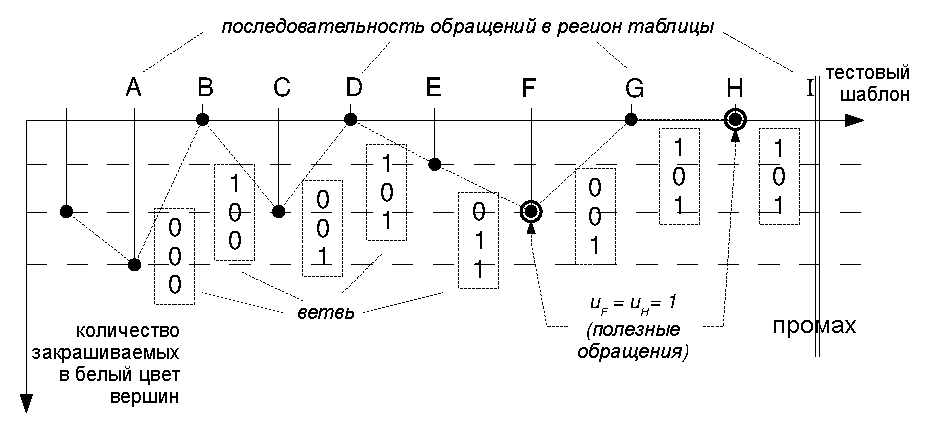
\includegraphics[width=\textwidth]{2.theor/plru_usefl_exmp}
  \caption{Перекрашивание ветви последовательностью обращений}\label{fig:plru_exmp_vytesn}
  \end{figure}

На рисунке~\ref{fig:plru_exmp_vytesn} изображен пример процесса перекрашивания для \\8-ассоциативной таблицы. В этом примере рассматривается ветвь, ведущая в строку, к которой происходит обращение А. После обращения к своей же строке вся ветвь становится белой: линия из А в В помечена (0 0 0)$^T$. Чем <<глубже>> по оси ординат происходит обращение, тем <<глубже>> становится белой ветвь (значение по оси ординат означает количество подряд вершин ветви, начиная с первой (самой верхней в векторах на рисунке), которые становятся равными нулю, а следующая за ней вершина, если она существует, становится равной единице, остальные вершины не меняются). Обращение В самое <<мелкое>>, оно лишь меняет первую вершину ветви, делая ее чёрной. Следующее обращение, С, перекрашивает 2 вершины в белый цвет (в том числе и ту вершину, которую только что обращение В покрасило в чёрный цвет) и 1 вершину в чёрный цвет. И так далее.

Обратим внимание на обращения F и H. Вершины, которые они закрашивают в чёрный цвет, сохраняют свой цвет до промаха, в котором будет определяться, вытеснять ли данную строку. Это происходит потому, что все следующие обращения происходят с закрашиванием меньшего числа вершин, чем F и H. В качестве функционала вытеснения рассмотрим количество таких обращений, как F и H, т.е. таких, после которых обращения закрашивают меньшее число вершин: самое большое число таких вершин есть длина ветви, самое малое - ноль (обращение А), изменений одной ветви определяется без отсылок к другим ветвям, вытеснение происходит тогда и только тогда, когда количество чёрных вершин равно длине ветви.

%Например, представленный на рисунке~\ref{fig:plru-useful} шаблон успевает
% покрасить 5 вершин ветви в черный цвет.
%
%\begin{figure}[t] \center
%  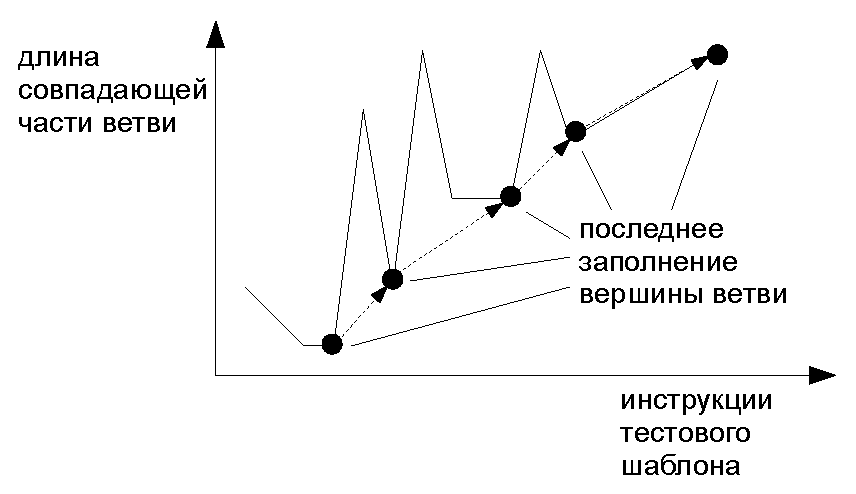
\includegraphics[width=0.6\textwidth]{2.theor/plru-useful}\\
%  \caption{Заполнение ветви черными вершинами в стратегии вытеснения
%  \PseudoLRU}\label{fig:plru-useful}
%\end{figure}

\begin{utv}
Обращение $I$ считается полезным в случае стратегии вытеснения \PseudoLRU, если все последующие обращения (до промаха, в котором вся ветвь будет чёрной) затрагивают только те вершины ветви, которые расположены выше вершины, перекрашиваемой инструкцией $I$ в черный цвет.
\end{utv}

Для вытеснения нужно не менее $\log_2 w$ полезных обращений (длина ветви). Далее выражение $\log_2 w$ будет обозначаться буквой $W$.

%Отличие этого функционала вытеснения от функционала для \LRU является \emph{немонотонность}. Это означает, что полезные инструкции надо считать для каждого промаха заново ---
%инструкции между двумя соседними промахами могут <<забелить>>
%несколько вершин ветви, что уменьшит функционал вытеснения
%(см.рис.~\ref{nonmonotonic}). Метрика для \LRU является монотонной,
%потому что инструкции между промахами не могут уменьшить функционал вытеснения -- либо не меняют, либо увеличивают ее, сдвигая ключ к концу вектора \LRU (см. рис.~\ref{monotonic}).
%
%%Таким образом, ограничение, описывающее стратегию вытеснения
%%\PseudoLRU, будет представлено дизъюнкцией ограничений по всем
%%предыдущим кэш-промахам.
%
%\begin{figure}[h] \center
%  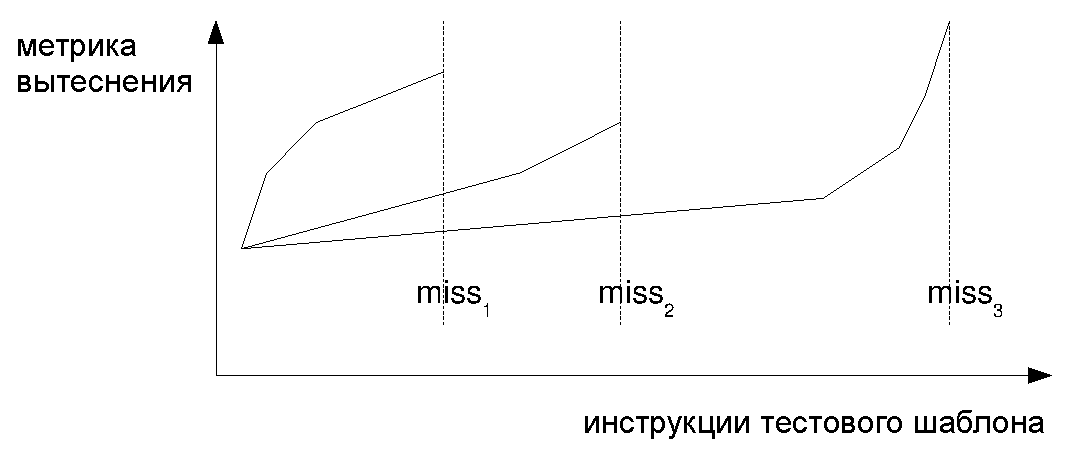
\includegraphics[width=0.6\textwidth]{2.theor/nonmonotonic}\\
%  \caption{Немонотонный функционал вытеснения}\label{nonmonotonic}
%\end{figure}
%
%\begin{figure}[h] \center
%  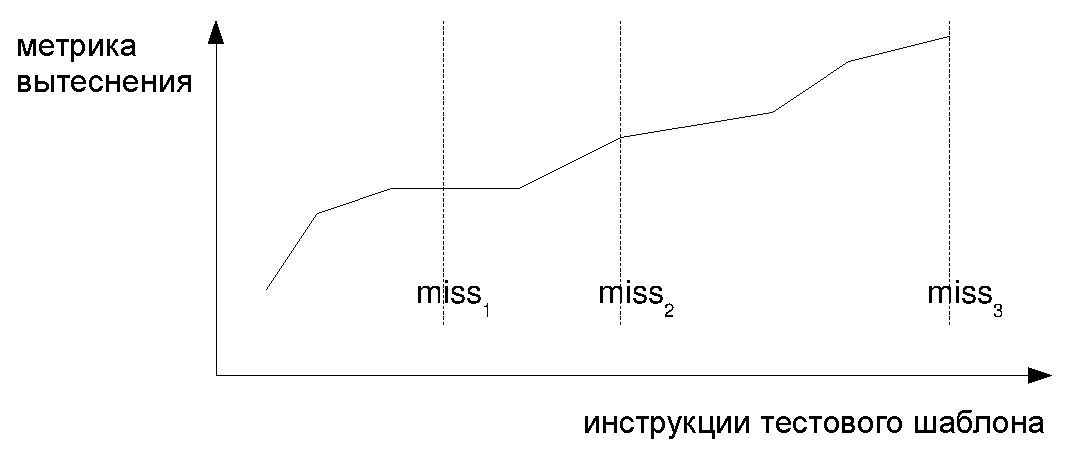
\includegraphics[width=0.6\textwidth]{2.theor/monotonic}\\
%  \caption{Монотонный функционал вытеснения}\label{monotonic}
%\end{figure}

Осталось записать формулу полезного обращения для \PseudoLRU в виде ограничений. Определимся с набором переменных. Каждому обращению в таблицу будут соответствовать следующие переменные:
\begin{itemize}
  \item ключ $k_i$;
  \item регион $R_i$;
  \item позиция $\pi_i$ (определение см. в разделе~\ref{sec:PseudoLRUonBranches}), $\pi_i \in \{0..w{-}1\}$;
  \item позиция $\pi'_i$ в момент последнего обращения перед данным (только для неинициализирующих обращений).
\end{itemize}

Обращение по ключу $k_i$ в регион $R_i$ на позицию $\pi_i$ будет полезным для вытеснения ключа $k_{n+1}$ в регионе $R_{n+1}$ ($i < n+1$) с позицией в момент последнего обращения $\pi'_{n+1}$, если выполнены все следующие условия (ниже будет доказано, что это определение соответствует стратегии вытеснения \PseudoLRU):
\begin{enumerate}
  \item <<$i$'е>> обращение происходит после последнего обращения к $k_{n+1}$ в $R_{n+1}$ перед $(n+1)$'м обращением;
  \item <<$i$'е>> обращение происходит в тот же регион, что и $R_{n+1}$;
  \item <<$i$'e>> обращение происходит до ближайшего повторного обращения на позиции $\pi'_{n+1}$;
  \item все обращения после <<$i$'го>> до ближайшего повторного обращения на позиции $\pi'_{n+1}$ просходит без закрашивания той вершины, которую красит <<$i$'e>> обращение.
\end{enumerate}

В момент последнего обращения по ключу $k_{n+1}$ в $R_{n+1}$ ветвь к нему становится целиком белой и начинается процесс вытеснения. Последующие инструкции перекрашивают эту ветвь до тех пор, пока не встретится обращение с промахом на той же позиции, которая была в момент последнего обращения к $k_{n+1}$ в $R_{n+1}$. К этому моменту вся ветвь должна стать чёрной, а после этого обращения ветвь вновь становится белой, но эта ветвь уже относится к другому ключу (тому, который вытеснил $k_{n+1}$).

Поясню этот момент с другой стороны. Рассматривая успешность очередного обращения к некоторому ключу, ищем ближайшее предыдущее обращение к тому же ключу (обращение А на рисунке~\ref{fig:plru_exmp_vytesn}). Обращения, идущие после этого <<предыдущего>>, либо должны вытеснить соответствующий ключ (если речь идёт о неуспешном обращении), либо не должны вытеснить (если --- об успешном). Если среди этих обращений не встречается обращение по той же позиции, что и в момент <<предыдущего>> обращения, то вытеснение не произойдет (т.к. в противном случае в этом обращении могло произойти бы вытеснение по определению \PseudoLRU). Если же обращение встречается (обращение I на рисунке~\ref{fig:plru_exmp_vytesn}), то к его моменту вся ветвь должна успеть стать полностью чёрной.

Переменные $\pi_i$ для позиций обладают собственными ограничениями, не зависящими от успешности обращений по ним. А именно, позиции --- это битовые строки длины $W$, идентифицирующие ключи: если позиции двух обращений совпадают и между ними нет промахов по этой позиции, то ключи должны совпадать, если же позиции различаются, то и ключи должны различаться (обозначим $t_i$ и $r_i$ --- ключи и регионы инициализирующих обращений, $k_i$ и $R_i$ --- ключи и регионы в обращениях из тестового шаблона, обозначим $s \equiv \langle (t_1||r_1), ..., (t_m||r_m), (k_1||R_1), ..., (k_n||R_n)\rangle$):

для каждой пары обращений $i$ и $j$ ($j$'е --- после $i$'го)
\begin{itemize}
    \item если $S_j$ = hit, то $$(\pi_i||R(s_i) = \pi_j||R(s_j)~\wedge$$ $$\pi_i||R(s_i) \notin \{\pi_{m_1}||R(s_{m_1}), \pi_{m_2}||R(s_{m_2}), \dots, \pi_{m_n}||R(s_{m_n})\}) \rightarrow s_i = s_j$$
    \item если $S_j$ = miss, то $$(\pi_i||R(s_i) = \pi_j||R(s_j)~\wedge$$ $$\pi_i||R(s_i) \notin \{\pi_{m_1}||R(s_{m_1}), \pi_{m_2}||R(s_{m_2}), \dots, \pi_{m_n}||R(s_{m_n})\}) \rightarrow s_i \neq s_j$$
\end{itemize}
где $(\pi_{m_1},R(s_{m_1})), (\pi_{m_2},R(s_{m_2})), \dots, (\pi_{m_n},R(s_{m_n}))$ --- позиции и регионы неуспешных обращений,
расположенных между $i$'м и $j$'м обращениями. В качестве $i$'го обращения также надо рассмотреть и инициализирующие обращения.

%% это "перевернутые"позиции! у них чем ближе к листу, тем дальше от левой границы в битовом представлении

И, наконец, определение для $\pi'_i$ в виде ограничений. Если $S_i$ = hit, то  $\pi'_i$ --- позиция в том обращении, где в последний раз встретился ключ $k_i$ в регионе $R_i$:
$$
\begin{array}{l}
\texttt{(ite~} ((k_i||R_i) = (k_{i-1}||R_{i-1})) ~~ (\pi'_i = \pi_{i-1})\\
\texttt{(ite~} ((k_i||R_i) = (k_{i-2}||R_{i-2})) ~~ (\pi'_i = \pi_{i-2})\\
... ~(\pi'_i = 0)\texttt{)))...)}\\
\end{array}
$$

Подформула $\pi'_i = 0$ не оказывает влияния, если $(k_i||R_i) \in \{(k_{i-1}||R_{i-1}),$ $(k_{i-2}||R_{i-2}), ... \}$, а так и будет

Если $S_i = $ miss, то кроме того, что $\pi'_i$ --- позиция последнего вхождения ключа $k_i$ в регионе $R_i$, надо убедиться, что та же позиция $\pi'_i$ встречается после последнего обращения к $k_i$ в $R_i$ на неуспешном обращении ( $\{\pi_i, ..., \pi_j\}_m$ обозначает подмножество множества позиций от $i$'го до $j$'го обращения из неуспешных обращений):
$$
\begin{array}{l}
\texttt{(ite~} ((k_i||R_i) = (k_{i-1}||R_{i-1})) ~~ (\pi'_i = \pi_{i-1})\\
\texttt{(ite~} ((k_i||R_i) = (k_{i-2}||R_{i-2})) ~~ (\pi'_i = \pi_{i-2} \wedge \pi'_i \in \{\pi_{i-1}\}_m)\\
\texttt{(ite~} ((k_i||R_i) = (k_{i-3}||R_{i-3})) ~~ (\pi'_i = \pi_{i-3} \wedge \pi'_i \in \{\pi_{i-1}, \pi_{i-2}\}_m)\\
... ~(\pi'_i = 0)\texttt{)))...)}\\
\end{array}
$$

Переходим непосредственно к записи формулы полезного обращения. Запишем каждое условие этого определения в виде ограничений ( $k_{n+1}$ и $R_{n+1}$ --- ключ и регион, по отношению к которым определяется вытеснение, $s \equiv \langle (t_1||r_1), ..., (t_m||r_m), (k_1||R_1), ..., (k_n||R_n)\rangle$ --- предыдущие обращения (ключи и регионы), $\sigma \equiv \langle (\tau_1||r_1), ..., (\tau_m||r_m), (\pi_1||R_1), ..., (\pi_n||R_n)\rangle$ --- предыдущие обращения (позиции и регионы), $i$ --- номер обращения, для которого записывается формула полезного обращения, $R(s_i)$ --- вторая компонента $s_i$, $R(\sigma_i)$ --- вторая компонента $\sigma_i$, $\pi(\sigma_i)$ --- первая компонента $\sigma_i$) :
\begin{enumerate}
    \item $(k_{n+1}||R_{n+1}) \notin \{s_i, s_{i+1}, ...,  s_{m+n}\}$ -- $i$'е обращение происходит после последнего обращения к $k_{n+1}$ в $R_{n+1}$;
    \item $R_{n+1} = R(s_i)$ -- обращение происходит в тот же регион;
    \item $(\pi'_{n+1}||R_{n+1}) \in \{\sigma_i, \sigma_{i+1}, ..., \sigma_{m+n}\}$ -- обращение происходит до ближайшего повторного обращения на ту же позицию;
    \item $\bigwedge\limits_{j = i+1}^n (((\pi'_{n+1}||R_{n+1}) \notin \{\sigma_i, \sigma_{i+1}, ..., \sigma_j\}~\wedge~R(\sigma_i) = R(\sigma_j)) \rightarrow P(\pi(\sigma_i) \oplus \pi'_{n+1}, \pi(\sigma_j) \oplus \pi'_{n+1}))$ --- полезные инструкции должны закрашивать больше белых вершин, чем закрашивают все последующие инструкции;  предикат $P$ для пары векторов $\delta_i$ и $\delta_j$ (<<относительных позиций>> --- см. раздел~\ref{sec:PseudoLRUonBranches}) истинен тогда и только тогда, когда количество старших нулевых бит у $\delta_i$ больше количества старших нулевых бит у $\delta_j$, иными словами, только и только тогда, когда существует целое $k$ такое, что $\delta_i < 2^k \leqslant \delta_j$ (см.рис.~\ref{fig:bits}); из леммы~\ref{QuantorElimination} (ее формулировка и доказательство находятся в приложении~\ref{sec:proofs}) следует, что этот предикат обладает бескванторной эквивалентной формой: $P(\delta_i, \delta_j) \equiv (\delta_j > \delta_i~~\wedge~~\delta_j \oplus \delta_i > \delta_i)$, сравнения беззнаковые.
\end{enumerate}

\begin{figure}[h] \center
  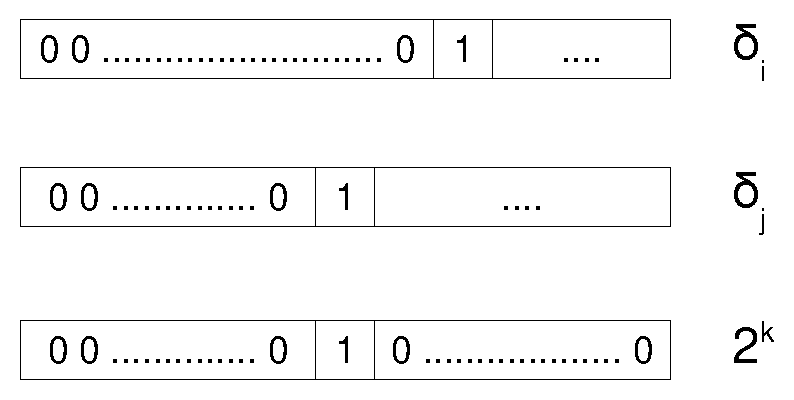
\includegraphics[width=0.4\textwidth]{2.theor/bits}\\
  \caption{Перекрашивание и битовые строки}\label{fig:bits}
\end{figure}

Итак, система ограничений для описания обращений по ключу $k_i$ в регион $R_i$ согласно методу полезных обращений для \PseudoLRU:
\begin{itemize}
\item для hit($k_i, R_i$):
$$
\left\{\begin{array}{l}
(k_i||R_i) \in \{(t_1||r_1), ..., (t_m||r_m), (k_1||R_1), ..., (k_{i-1}||R_{i-1})\}\\
\{(t_1||r_1), ..., (t_m||r_m)\} - \mbox{все разные}\\
\sum\limits_{j=1}^m [u_{k_i,R_i,\pi'_i}(t_j||r_j)] + \sum\limits_{j=1}^{i-1} [u_{k_i,R_i,\pi'_i}(k_j||R_j)] < W\\
\end{array} \right.
$$
\item для miss($k_i, R_i$):
$$
\left\{\begin{array}{l}
(k_i||R_i) \in \{(t_1||r_1), ..., (t_m||r_m), (k_1||R_1), ..., (k_{i-1}||R_{i-1})\}\\
\{(t_1||r_1), ..., (t_m||r_m)\} - \mbox{все разные}\\
\sum\limits_{j=1}^m [u_{k_i,R_i,\pi'_i}(t_j||r_j)] + \sum\limits_{j=1}^{i-1} [u_{k_i,R_i,\pi'_i}(k_j||R_j)] \geqslant W\\
\end{array} \right.
$$
\end{itemize}

$$u_{k_i,R_i,\pi'_i} (s_j)  \equiv \left\{\begin{array}{l}
(k_i||R_i) \notin \{s_j, s_{j+1}, ..., s_{m+n}\}\\
R_i = R(s_j)\\
(\pi'_i||R_i) \in \{(\pi_j||R_j), (\pi_{j+1} || R_{j+1}), ..., (\pi_{m+n}||R_{m+n})\}\\
\bigwedge\limits_{l = j+1}^{m+n} (R_j = R_l ~\wedge~(\pi'_i||R_i) \notin \{(\pi_j||R_j), (\pi_{j+1}||R_{j+1}), ..., (\pi_l||R_l)\}\\
 \hspace{2cm} \rightarrow P(\pi_j \oplus \pi'_i, \pi_l \oplus \pi'_i))\\
\end{array}\right.
$$
$$s \equiv \langle (t_1,r_1), (t_2,r_2), ..., (t_m,r_m), (k_1, R_1), ..., (k_n,R_n) \rangle$$
$$R(s_i) \mbox{~--- вторая компонента~} s_i$$
$$P(x, y) \equiv (y > x~~\wedge~~x \oplus y > x)$$


%Таблица~\ref{plru_table} содержит ограничения для разных случаев
%кэш-попаданий и кэш-промахов (см. утверждение~\ref{hit_miss_human}).
%В каждое из них включается ограничение на количество полезных
%инструкций согласно предлагаемой методике использования функций
%полезности. Полезности считаются относительно некоторого кэш-промаха
%(для их перебора используется сокращение $x_m : \mbox{miss}$).

В приложении~\ref{sec:proofs} доказана теорема~\ref{PLRUusefulThm} эквивалентности этих формул определению стратегии вытеснения \PseudoLRU.

Немного изменив формулу для $\pi'_i$, можно упростить ограничения \textbf{для}\\ \textbf{успешных} обращений. А именно, определив $\pi'_i$ так:

$$
\begin{array}{l}
\texttt{(ite~} (s_i = s_{i-1}) ~~ (\pi'_i = \pi_{i-1})\\
\texttt{(ite~} (s_i = s_{i-2}) ~~ (\pi'_i = \pi_{i-2} \wedge \pi'_i \neq \pi_{i-1})\\
...\\
\texttt{(ite~} (s_i = s_j) ~~ (\pi'_i = \pi_j \wedge \pi'_i \notin \{\pi_{j+1}, ..., \pi_{i-1}\})\\
... \texttt{~true )))...)}\\
\end{array}
$$

для hit($k_i, R_i$) будет достаточно таких ограничений:
$$
\left\{\begin{array}{l}
(k_i||R_i) \in \{(t_1||r_1), ..., (t_m||r_m), (k_1||R_1), ..., (k_{i-1}||R_{i-1})\}\\
\{(t_1||r_1), ..., (t_m||r_m)\} - \mbox{все разные}\\
\end{array} \right.
$$
т.е. ограничение на сумму будет автоматически выполнено. Этот факт следует из того, что о возможности вытеснения можно вести речь там, где встречается хотя бы одно неуспешное обращение на позиции $\pi'_i$. Если же позиция $\pi'_i$ не встречается после последнего обращения к ключу $k_i$, то и вытеснение произведено не будет (в формулах полезных обращений третье условие ложно для всех $s_j$, значит, количество полезных обращений равно равно 0, что означает невытеснение).

\subsection{Разрешение ограничений, описывающих стратегии вытеснения}

Ограничения, которые предлагается строить для описания количества полезных обращений, являются \emph{ограничениями мощности} (cardinality constraints). Это
ограничения вида $C_1 \leqslant \sum_{i=1}^n a_i \leqslant C_2$, где $C_1, C_2$
-- неотрицательные целые числа, а $a_i$ принимают значения 0 или
1~\cite{smt_debugging, PiskacK08, KuncakR07,
Revesz05}. Речь идет об ограничении размера некоторого множества
элементов, заданного с помощью характеристической функции.
В~\cite{smt_debugging} проведено исследование способов записи
ограничений мощности и показано, что от формы записи зависит
эффективность разрешения этих ограничений. Одна из таких форм рассматривает ограничения
мощности как компактную форму записи уравнения
вида $\bigvee_{C_1 \leqslant C \leqslant C_2} \sum_{i=1}^n a_i = C$,
где равенство есть
\begin{itemize}
\item тождественная ложь, если $C < 0$ или $C > n$;
\item конъюнкция $\bigwedge_{1\leqslant i\leqslant n} (a_i = 0)$,
если $C = 0$;
\item дизъюнкция по всевозможным выборкам индексов $i_1, ..., i_C$, где
для каждого индекса $i_k$ справедливы свойства $1 \leqslant i_k
\leqslant n$ и $i_k < i_{k+1}$, конъюнкций $\bigwedge_{i_k} (a_{i_k}
= 1)$, если $1 \leqslant C \leqslant n$.
\end{itemize}

В диссертации не ставилась задача исследования способов разрешения ограничений
мощности (с целью выбора наиболее эффективного способа их представления). Вместо
этого были использованы
имеющиеся инструменты разрешения ограничений мощности~\cite{Z3, Yices}. Для
записи оставшихся формул был использован язык битовых строк, для разрешения
ограничений над которым существуют эффективные SMT-инструменты (например,
Z3~\cite{Z3}).

%После устранения ограничений мощности в формуле остаются только
%ограничения на конечные множества тегсетов: принадлежности и
%непринадлежности тега конечному множеству тегсетов и равенства и
%неравенства битовых полей тегсетов. Поскольку конечные множества
%тегсетов известны (заданы перечислением тегсетов, которые в входят в
%это множество), то ограничения принадлежности и непринадлежности
%могут быть переписаны без использования этих отношений. Отношение
%принадлежности $x \in \{x_1, x_2, ..., x_n\}$ может быть переписано
%в виде дизъюнкции $(x = x_1) \vee (x = x_2) \vee ... \vee (x =
%x_n)$, а отношение непринадлежности $x \notin \{x_1, x_2, ...,
%x_n\}$ -- в виде конъюнкции $(x \neq x_1) \wedge (x \neq x_2) \wedge
%... \wedge (x \neq x_n)$.
%
%В результате получается предикат, в котором переменными величинами
%являются неотрицательные целые числа с конечной областью значений
%(тегсеты), над переменными возможны операции получения битового
%поля, в предикате используется отношение равенства и неравенства над
%битовыми полями. Кроме того, этот предикат задается с использованием
%ограничений мощности.
%
%Для разрешения такого рода предикатов можно было бы разрабатывать
%собственные процедуры распространения ограничений, но это свело бы
%на нет все усилия по выработке собственного представления стратегии
%вытеснения. Однако предлагаемые ограничения могут быть тривиальным
%образом выражены на языке теорий, для которых существуют эффективные
%разрешающие процедуры (битовые строки, неинтерпретируемые функции).
%Поэтому для записи и разрешения этих ограничений могут быть
%использованы SMT-инструменты~\cite{Z3}.

%%%%%%%%%%%%%%%%%%%%%%%%%%%%%%%%%%%%%%%%%%%%%%%%%%%%%%%%%%%%%%%%%%%
%
%\pagebreak
%\section{Ограничения, описывающие тестовые ситуации в некоторых
%частных случаях, для стратегии вытеснения \LRU}
%
%\subsection{Тестовые шаблоны без кэш-промахов}
%
%В случае тестовых шаблонов, в которых нет кэш-промахов, нет ни
%вытесняющих, ни вытесняемых тегсетов. Поэтому в таких шаблонов
%уравнения для кэш-попаданий имеют очень простой вид:
%
%$$
%\left\{
%\begin{array}{l}
%x \in D\\
%... (\mbox{тестовые ситуации на остальные буферы})\\
%\end{array}
%\right.
%$$
%
%\subsection{Тестовые шаблоны без кэш-попаданий}
%
%В случае тестовых шаблонов, в которых нет кэш-попаданий, надо
%генерировать ограничения для вытесняющих и лишь иногда для
%вытесняемых тегсетов. А именно, вытесняемый тегсет требуется лишь в
%том случае, когда кэш-промах вносит в кэширующий буфер ранее
%вытесненный тегсет. В этом случае для вытесняемого тегсета известен
%домен, что позволяет построить уравнения обозримого размера. Кроме
%того, поскольку отсутствуют кэш-попадания, повторные обращения к
%вытесняемым тегсетам (кроме кэш-промаха, который их может внести в
%кэширующий буфер) невозможны, что также упрощает генерируемые
%уравнения.
%
%В результате получается, что вытесняющий тегсет описывается в
%тестовом шаблоне без кэш-попаданий следующей системой уравнений:
%$$
%F'(x) \vee F''(x) \vee \bigvee_{\lambda_\delta \in D} F'''(x, \lambda_\delta)
%$$
%
%где
%
%$$F'(x) \equiv (x \notin D \wedge x \notin \{x_1, ..., x_n\})$$
%
%$$F''(x) \equiv (x \in \{x_1, ..., x_n\} \wedge \sum_{i=1}^n u''(x_i) \geqslant w)$$
%
%$$u''(x_i) \equiv (x\notin \{x_i, ..., x_n\} \wedge R(x_i) = R(x))$$
%
%$$F'''(x, \lambda_\delta) \equiv (x = \lambda_\delta \wedge x \notin
%\{x_1, ..., x_n\} \wedge \sum_{i=1}^n (R(x_i) = R(x)) \geqslant w -
%\delta + 1)$$
%
%\subsection{Короткие тестовые шаблоны}
%
%Будем называть тестовый шаблон \emph{коротким}, если в нем не более
%$w$ инструкций обращения к памяти. Очевидно, что любой короткий
%тестовый шаблон является простым. Из 7 случаев для коротких тестовых
%шаблонов остается всего 5 (первые два можно еще объединить в более
%компактную систему уравнений). В таблице~\ref{short_templates_table}
%предъявлены функции полезности и ограничения для коротких тестовых
%шаблонов в случае стратегии вытеснения \LRU. Соответствующая теорема
%корректности этих ограничений сформулирована и доказана в
% приложении~\ref{sec:proofs}.
%
%\begin{table}[t]
%\begin{tabular}{|c|c|c|c|}
%\hline  & \centering случай &
%\begin{tabular}{c}переменная\\перебора\end{tabular} & система \\
%\hline \hline \multirow{-2}{*}{\rotatebox{90}{кэш-попадание}} &
%\makecell[c{p{0.3\textwidth}}]{тегсет находится в начальном
%состоянии буфера и он всё ещё не вытеснен} & $\lambda_\delta \in D$
%&
%$\left\{\begin{array}{l} x = \lambda_\delta\\
%\sum\limits^n_{i=1} u(x_i) \leqslant w - \delta
%\end{array}\right.$ \\ \hhline{~|---}
%& \makecell[c{p{0.3\textwidth}}]{тегсет уже встречался в шаблоне} &
%-- & $x \in \{x_1, ..., x_n\}$
%\\ \hline \hline \multirow{6}{*}{\rotatebox{90}{кэш-промах}}
%& \makecell[c{p{0.3\textwidth}}]{тегсет встречается впервые} & -- &
%$\left\{\begin{array}{l} x \notin D\\
%x \notin \{x_1, ..., x_n\}\\
%\end{array}\right.$\\ \hhline{~|---} &
%\makecell[c{p{0.3\textwidth}}]{тегсет находился в начальном
%состоянии буфера и был вытеснен} & $\begin{array}{c}\lambda_\delta
%\in D,\\\delta \geqslant w-n+1\end{array}$ &
%$\left\{\begin{array}{l} x = \lambda_\delta\\
%x \notin \{x_1, ..., x_n\}\\
%\sum\limits^n_{i=1} u(x_i) > w - \delta\\
%\end{array}\right.
%$ \\ \hline
%\end{tabular}
%
%%где функция полезности определена следующим образом:
%$$u(x_i) \equiv
%\left\{\begin{array}{l} x_i \in \{ \lambda_{\delta+1}, ...,
%\lambda_w\}~\wedge~x_i \notin \{x_1, ..., x_{i-1}\}, \mbox{если}~S_i
%= \mbox{hit}\\
%R(x_i) = R(x), \mbox{если}~S_i = \mbox{miss}
%\end{array}\right.
%$$
%\caption{Таблица систем уравнений для тестовых ситуаций в кэширующих
%буферах для коротких тестовых шаблонов в случае стратегии вытеснения
%\LRU}\label{short_templates_table}
%\end{table}
%
%
%
%%\begin{landscape}
%%\begin{table}
%%\begin{tabular}{|c|c|c|c|c|c|}
%%\hline  & \centering случай &
%%\begin{tabular}{c}переменная\\перебора\end{tabular} & система &
%%\begin{tabular}{c}функция\\полезности\\для кэш-\\попадания\end{tabular} &
%%\begin{tabular}{c}функция\\полезности\\для кэш-\\промаха\end{tabular} \\
%%\hline \hline \multirow{-2}{*}{\rotatebox{90}{кэш-попадание}} &
%%\makecell[c{p{0.3\textwidth}}]{тегсет находится в начальном
%%состоянии буфера и он всё ещё не вытеснен} & $\lambda_\delta \in
%%D$ &
%%$\left\{\begin{array}{l} x = \lambda_\delta\\
%%\sum\limits^n_{i=1} u(x_i) \leqslant w - \delta
%%\end{array}\right.
%%$ &
%%\begin{tabular}{c}
%%$x_i \in \{ \lambda_{\delta+1}, ..., \lambda_w\}$\\
%%$\wedge~x_i \notin \{x_1, ..., x_{i-1}\}$
%%\end{tabular}
%%& $R(x_i) = R(x)$
%%\\ \hhline{~|-----}
%%& \makecell[c{p{0.3\textwidth}}]{тегсет уже встречался в шаблоне} &
%%-- & $x \in \{x_1, ..., x_n\}$ & -- & --
%%\\ \hline \hline \multirow{6}{*}{\rotatebox{90}{кэш-промах}}
%%& \makecell[c{p{0.3\textwidth}}]{тегсет встречается впервые} & -- &
%%$\left\{\begin{array}{l} x \notin D\\
%%x \notin \{x_1, ..., x_n\}\\
%%\end{array}\right.
%%$ & -- & -- \\ \hhline{~|-----} &
%%\makecell[c{p{0.3\textwidth}}]{тегсет находился в начальном
%%состоянии буфера и был вытеснен} &
%%$\begin{array}{c}\lambda_\delta \in D,\\\delta \geqslant
%%w-n+1\end{array}$ &
%%$\left\{\begin{array}{l} x = \lambda_\delta\\
%%x \notin \{x_1, ..., x_n\}\\
%%\sum\limits^n_{i=1} u(x_i) > w - \delta\\
%%\end{array}\right.
%%$ &
%%\begin{tabular}{c}
%%$x_i \in\{\lambda_{\delta+1}, ..., \lambda_w\}$\\
%%$\wedge~x \notin \{x_1, ..., x_{i-1}\}$\\
%%\end{tabular}
%%&
%%\begin{tabular}{c}
%%$R(x_i) = R(x)$\\
%%\end{tabular}
%%\\ \hline
%%\end{tabular}
%%\caption{Таблица систем уравнений для тестовых ситуаций в кэширующем буфере
%%для коротких тестовых шаблонов в случае стратегии вытеснения
%%\LRU}\label{short_templates_table}
%%\end{table}
%%\end{landscape}
%
%
%\subsection{Генерация тестовых данных для кэш-памяти, содержащей
%<<грязные>> ячейки}
%
%Любая ячейка в кэш-памяти может быть помечена \emph{грязной}
%(\emph{invalid}). Это означает, что данные, находящиеся в кэширующем
%буфере по этому адресу, не могут использоваться в качестве данных,
%хранящихся в памяти по этому адресу.
%
%Рассмотренные ранее в этой работе случаи не учитывали грязные ячейки
%кэширующем буфере, хотя они зачастую присутствуют в микропроцессоре
%после его запуска -- с таким состоянием кэширующего буфера работают
%первые после запуска микропроцессора инструкции.
%
%Кэш-попадание возникает в том случае, когда требуемые данные
%присутствуют среди <<чистых>> ячеек кэширующего буфера. Кэш-промах
%возникает в том случае, когда требуемых данных нет среди <<чистых>>
%ячеек. Причем при наличии <<грязных>> ячеек вытеснения может и не
%произойти. А именно, если все ячейки набора, с которым работает
%инструкция, являются <<чистыми>>, то происходит вытеснение согласно
%стратегии вытеснения, остальные наборы не меняются. Если же среди
%ячеек набор есть <<грязные>> ячейки, то вытеснение не происходит, а
%на место одной из <<грязных>> ячеек помещаются данные из основной
%памяти по заданному адресу и ячейка объявляется <<чистой>>.
%Остальные ячейки не меняются. В стратегии вытеснения \LRU эта бывшая
%<<грязная>> ячейка становится самой новой.
%
%Для генерации тестовых данных для кэширующих буферов с грязными
%ячейками предлагается применять ограничения с функциями полезности.
%Примечательно, что наличие грязных ячеек не меняет качественно
%систему уравнений.
%
%В данном разделе рассматривается случай, когда начальное состояние
%микропроцессора известно. Кроме того, рассматриваемый случай
%учитывает отсутствие инструкций в тестовом шаблоне, которые
%превращали бы <<чистые>> ячейки в <<грязные>> (т.е. все такие
%изменения должны делаться явно вне тестовых шаблонов).
%
%\subsubsection{случай полностью-ассоциативного кэширующего буфера}
%
%В случае полностью-ассоциативных кэширующих буферов очевидно, что
%первые кэш-промахи будут заполнять <<грязные>> ячейки. Пусть $N$ --
%количество <<грязных>> ячеек в начальном состоянии кэширующего
%буфера, а $L_0$ -- начальное состояние (выражение) кэширующего
%буфера (только <<чистые>> ячейки). Тогда для тестовых ситуаций надо
%генерировать такие ограничения ($L$ -- выражение для состояния
%кэширующего буфера перед исполнением инструкции, $L'$ -- выражение
%для состояния кэширующего буфера после исполнения инструкции):
%\begin{itemize}
%\item для \emph{кэш-попадания} hit($x$) генерируются ограничения
%$$
%\left\{
%\begin{array}{l}
%x \in L\\
%L' \equiv L\\
%\end{array}
%\right.
%$$
%
%\item для \emph{кэш-промаха} miss($x$), если это один из первых $N$
%кэш-промахов, генерируются ограничения:
%$$
%\left\{
%\begin{array}{l}
%x \notin L\\
%L' \equiv L \cup \{x\}\\
%\end{array}
%\right.
%$$
%
%\item для \emph{кэш-промаха} miss($x$), являющегося по счету более
%чем $N$'м кэш-промахом тестового шаблона, генерируются ограничения:
%$$
%\left\{
%\begin{array}{l}
%x \notin L\\
%x' \in L\\
%L' \equiv L\setminus\{x'\} \cup \{x\}\\
%displaced(x', L)\\
%\end{array}
%\right.
%$$
%\end{itemize}
%
%Предикат $displaced(x', L)$ истинен, если $x'$ является вытесняемым
%тегом в текущем состоянии кэширующего буфера $L$. Для стратегии
%вытеснения \LRU этот предикат может быть записан с использованием
%тех же диапазонов вытеснения, что и для кэширующего буфера без
%<<грязных>> ячеек (см.п.~\ref{LRU_constraints}). А именно, диапазон
%вытеснения начинается на инструкции, которая последний раз перед
%вытеснением тега обращается к нему. Тогда между этой инструкцией и
%инструкцией, вытесняющей $x$, должны быть обращения ко всем
%остальным тегам текущего состояния кэширующего буфера. Эта логика
%может быть записана в виде тех же уравнений, что и в
%пункте~\ref{LRU_constraints}. Нетрудно проверить, что для
%кэширующего буфера с <<грязными>> ячейками остается справедливой
%лемма о невложенных диапазонах вытеснения, что доказывает
%корректность использования ограничений из
%пункта~\ref{LRU_constraints} для кэширующего буфера с <<грязными>>
%ячейками.
%
%\subsubsection{случай наборно-ассоциативного кэширующего буфера}
%
%В этом пункте будет показано, что ограничения для кэширующего
%буфера, начальное состояние которого содержит <<грязные>> ячейки,
%качественно не отличаются от ограничений для кэширующего буфера без
%<<грязных>> ячеек.
%
%Аналогично тому, как это делалось для кэширующих буферов без
%<<грязных>> ячеек, для тестовых ситуаций на кэширующие буферы с
%<<грязными>> ячейками тоже возможно следующее исчерпывающее
%выделение случаев:
%\begin{itemize}
%\item кэш-попадание тега:
%    \begin{enumerate}
%    \item данный тег находился в начальном состоянии кэширующего буфера и не был
%    вытеснен к моменту данной инструкции;
%    \item данный тег был внесен в кэширующий буфер одной из инструкций
%    кэш-промаха и с тех пор не был вытеснен;
%    \end{enumerate}
%\item кэш-промах тега:
%    \begin{enumerate}
%    \item данный тег не встречался ранее (не находился в начальном
%    состоянии кэширующего буфера и не был внесен какими-либо кэш-промахами);
%    \item данный тег был ранее вытеснен из кэширующего буфера и с тех пор
%    не был внесен в кэширующий буфер вновь.
%    \end{enumerate}
%\end{itemize}
%
%Соответствующие ограничения приведены в
%таблице~\ref{dirty_hit_miss_table}.
%
%
%В таблице~\ref{dirty_hit_miss_table} символ $\Delta$ означает
%количество <<чистых>> ячеек в начальном состоянии того региона, про
%который идет речь в уравнении. На самом деле $\Delta$ есть функция
%региона ($\Delta = \Delta(\lambda_\delta)$), но для сокращения
%записи оставлен только функциональный символ. Кроме того, в
%приведенных уравнениях домен переменной включает только <<чистые>>
%ячейки.
%
%Сходства уравнений (со случаем кэширующих буферов без <<грязных>>
%ячеек) удалось добиться за счет рассмотрения <<грязных>> ячеек, как
%ячеек с наименьшим счетчиком \LRU, которые не участвуют в
%определении нахождения тега в кэширующих буферах. Поэтому в функциях
%полезности участвуют множества не $\{\lambda_{\delta+1}, ...,
%\lambda_w\}$, а множества $\{\lambda_{\delta+1}, ...,
%\lambda_\Delta\}$. Все <<чистые>> ячейки получили первые индексы,
%т.е. индексы всех от 1 до $\Delta$.
%
%%\begin{theorem}[корректность использования функций полезности для
%%записи \LRU в случае наличия <<грязных>> ячеек в начальном состоянии
%%кэширующего буфера] Тестовая программа, построенная по ограничениям,
%%которые сгенерированы с использованием предъявленных в
%%таблице~\ref{dirty_hit_miss_table} функций полезности, в случае
%%наличия <<грязных>> ячеек в начальном состоянии кэширующего буфера
%%удовлетворяет своему тестовому шаблону.
%%\end{theorem}
%%\begin{proof}
%%  //TODO
%%\end{proof}
%
%Для приведенных ограничений также могут быть применены эвристики,
%сокращающие их количество, которые были упомянуты для кэширующих
%буферов без <<грязных>> ячеек. Кроме того, в данном случае возможна
%дополнительная эвристика \emph{ограничение на $\delta$}: если
%$\delta + 1 < \Delta$, то функция полезности, в которую входит
%множество $\{\lambda_{\delta+1}, ..., \lambda_\Delta\}$, равна 0.
%
%%\subsection{Функции полезности для зеркальной генерации тестовых
%%данных}
%%
%%Рассмотрим ограничения, генерируемые для тестовых шаблонов
%%зеркальным методом с использованием функций полезности. По сравнению
%%с представленными ограничениями (см. табл.~\ref{hit_miss_table})
%%зеркальная генерация имеет свои особенности:
%%\begin{enumerate}
%%  \item множества констант (как, например, $L, D$) не используются,
%%  поэтому в ограничениях будут отсутствовать соответствующие им
%%  случаи;
%%  \item так как теги инструкций тестового шаблона должны появиться
%%  среди инициализирующей последовательности, то для вытеснения
%%  требуется $w-1$ инструкций, где $w$ -- ассоциативность кэширующего буфера;
%%  \item учет полезных инструкций начинается уже в инициализирующей
%%  последовательности, тем самым необходимо сформулировать функцию
%%  полезности для инициализирующих инструкций.
%%\end{enumerate}
%%
%%Следующая теорема описывает функцию полезности для инициализирующих
%%инструкций и описывает ограничения, генерируемые для тестовых
%%шаблонов зеркальным методом с использованием функций полезности
%%(количество инициализирующих инструкций зафиксировано, оно будет
%%обозначено параметром $m$):
%%
%%\begin{theorem}[Корректность ограничений, генерируемые зеркальным методом с
%%использованием функций полезности для
%%\LRU]\label{correct_mirror_LRU} Пусть $t_1, t_2, ..., t_m$ -- теги
%%инициализирующей последовательности, $x$ -- текущий тег тестового
%%шаблона, $x_1, x_2, ..., x_n$ -- теги предыдущих инструкций
%%тестового шаблона, причем $x \in \{t_1, ..., t_m, x_1, ..., x_n\}$ и
%%$\{t_1, ..., t_m\}$ --- все разные. Тогда $x$ не вытеснен согласно
%%определению на списках тогда и только тогда, когда
%%$$\sum\limits_{i=1}^{m+n} u_x(s_i) < w$$
%%где последовательность $s \equiv \langle t_1, ..., t_m, x_1, ...,
%%x_n\rangle$, а функция полезности определена следующим образом:
%%$$u_x(s_i) \equiv (x \notin \{s_i, ..., s_{m+n}\} \wedge
%%R(x) = R(s_i) \wedge s_i \notin\{s_{i+1},..., s_{m+n}\})$$
%%
%%%$$\sum\limits_{i=1}^m \tilde{u}_x(t_i) + \sum\limits_{i=1}^n u_x(x_i) < w$$
%%%где функции полезности определены следующим образом:
%%%$$\begin{array}{c}
%%%\tilde{u}_x(t_i) \equiv (x \notin \{t_i, ..., t_m, x_1, ..., x_n\}
%%%\wedge R(x) = R(t_i))\\u_x(x_i) \equiv (x \notin \{x_i, ..., x_n\}
%%%\wedge R(x) = R(x_i))\end{array}$$
%%
%%%$$\begin{array}{c}u_x(x_i) \equiv (x \notin \{x_i, ..., x_n\} \wedge R(x) =
%%%R(x_i)), \mbox{если}~S_i=\mbox{miss}\end{array}$$
%%%$$\begin{array}{c}u_x(x_i) \equiv (x \notin \{x_i, ..., x_n\} \wedge R(x) =
%%%R(x_i) \wedge \sum\limits_{j=1}^{m} \tilde{c}_{x_i}(t_j) = 0
%%%\wedge \sum\limits_{j=1}^{i-1} c_i(x_j) = 0),\\
%%%\mbox{если}~S_i=\mbox{hit}\end{array}$$
%%%$$c_i(x_j) \equiv (x \notin \{x_j, ..., x_{i-1}\} \wedge x_i = x_j)$$
%%%$$\tilde{c}_{x_i}(t_j) \equiv (x \notin \{t_j, ..., t_m, x_1, ..., x_{i-1}\} \wedge x_i = t_j)$$
%%\end{theorem}
%%\begin{proof}
%%//TODO написать правильное доказательство
%%
%%сумма полезных - это количество различных тегов, тогда полезными будем считать
% инструкции тестового шаблона, которые обращаются к разным тегам, при этом ко
% всем различным тегам есть инструкция; различные - например, последние; отсюда и
% функция полезности.
%%
%%%Воспользуемся леммой~\ref{hit_II}. При этом в качестве
%%%последовательности тегов тестового шаблона в этой лемме рассмотрим
%%%последовательность $t_1, t_2,~\dots,~t_m,~x_1,~x_2,~\dots,~x_n$.
%%%Согласно лемме тестовая ситуация на $x$ выполнена при
%%%соответствующем условии на сумму функций полезности от элементов
%%%этой последовательности. Функции полезности для
%%%$x_1,~x_2,~\dots,~x_n$ без изменений переходят из формулировки
%%%леммы~\ref{hit_II} в данную теорему. Функцию полезности для $t_1,
%%%t_2,~\dots,~t_m$ из формулировки леммы~\ref{hit_II} получить нельзя,
%%%поскольку неизвестна тестовая ситуация на эти теги. Однако, вспомнив
%%%определение полезной инструкции, функцию полезности для этих тегов
%%%получить несложно. А именно, тег $t_i$ будет полезным, если он
%%%продвигает $x$ к концу списка \LRU после последнего обращения к $x$.
%%%Если после последнего обращения к $x$ сам тег $t_i$ встречается
%%%впервые, то он будет полезным (см. доказательство
%%%леммы~\ref{hit_II}). Если же после последнего обращения к $x$ $t_i$
%%%встречается не в первый раз, то он не двигает $x$ к концу списка,
%%%что, тем самым, означает бесполезность $t_i$. Но поскольку все $t_i$
%%%разные, то повторное обращение возможно лишь среди
%%%$x_1,~x_2,~\dots,~x_n$ -- поэтому в функцию полезности для этих
%%%тегов добавлено отличие от $t_1,~t_2,~\dots,~t_m$.
%%\end{proof}
%%%\begin{sld}[Корректность ограничений, генерируемые зеркальным методом с
%%%использованием функций полезности для полностью ассоциативного \LRU
%%%буфера] Пусть $t_1, t_2, ..., t_m$ -- теги инициализирующей
%%%последовательности, $x$ -- текущий тег тестового шаблона, $x_1, x_2,
%%%..., x_n$ -- теги предыдущих инструкций тестового шаблона, причем $x
%%%\in \{t_1, ..., t_m, x_1, ..., x_n\}$ и $\{t_1, ..., t_m\}$ --- все
%%%разные. Тогда $x$ не вытеснен из полностью ассоциативного буфера
%%%согласно определению на списках тогда и только тогда, когда
%%%$$x \in \{s_{m+n-w+1}, ..., s_{m+n}\}$$ где последовательность $s
%%%\equiv \langle t_1, ..., t_m, x_1, ..., x_n\rangle$.
%%%\end{sld}
%%%\begin{proof}
%%%  //TODO
%%%\end{proof}
%%
%%Из теоремы~\ref{correct_mirror_LRU} следует система уравнений для
%%описания тестовой ситуации $S$ тега $x$, генерируемая зеркальным
%%методом с использованием функций полезности для \LRU (функции
%%полезности приведены в формулировке
%%теоремы~\ref{correct_mirror_LRU}):
%%\begin{itemize}
%%\item если $S$ = hit, то
%%$$
%%\left\{\begin{array}{l} x \in \{t_1, ..., t_m, x_1, ..., x_n\}\\
%%\sum\limits_{i=1}^m u_x(t_i) + \sum\limits_{i=1}^n u_x(x_i) < w\\
%%\{t_1, ..., t_m\} - \mbox{все разные}\\
%%\end{array} \right.
%%$$
%%\item если $S$ = miss, то
%%$$
%%\left\{\begin{array}{l} x \in \{t_1, ..., t_m, x_1, ..., x_n\}\\
%%\sum\limits_{i=1}^m u_x(t_i) + \sum\limits_{i=1}^n u_x(x_i)
%%\geqslant w\\
%%\{t_1, ..., t_m\} - \mbox{все разные}\\
%%\end{array} \right.
%%$$
%%\end{itemize}
%%
%%%Стоит заметить, что функции полезности добавили новое дополнительное
%%%условие на теги инициализирующих инструкций: они должны быть
%%%различными. В этом выражается свойство <<простоты>> инициализирующей
%%%последовательности, эта последовательность не должна содержать
%%%сложной внутренней последовательности изменений состояния
%%%кэширующего буфера.


\section{Конструирование тестовой программы для кэш-памяти первого и второго
уровня}\label{sec:L1L2_initialization}

В результате разрешения ограничений для каждой таблицы будет сгенерирована инициализирующая последовательность ключей, регионов и данных. Как уже было сказано, задачей
конструктора тестовых программ является построение инструкций микропроцессора,
которые осуществляют вычисленные обращения. Для написания конструктора тестовых
программ надо выяснить из документации по архитектуре способы исполнения
инструкций, при которых задействованы различные таблицы. Если для таблицы
нашлась инструкция, которая может произвести в нее обращение независимо от
других таблиц (это наиболее частый случай), то эту инструкцию и рекомендуется использовать в конструкторе. Более сложный
случай --- если такой инструкции найти не удается. В данном разделе будет
показан один такой случай и возможное поведение конструктора тестовой программы
для него.

Речь идет о кэш-памяти первого и второго уровня. Если обращение в кэш-память
первого уровня оказывается успешным, то обращение в кэш-память
второго уровня не производится. Получается, что последовательность обращений в
кэш-память второго уровня влияет на последовательность обращений в кэш-память
первого уровня: чтобы произошло обращение в кэш-память второго уровня, обращение
в кэш-память первого уровня должно быть неуспешным; и, наоборот, при неуспешном
обращении в кэш-память первого уровня возможно обращение в кэш-память второго
уровня (которое может нарушить построенную инициализирующую последовательность
для нее), правда, обращение к кэш-память второго уровня некоторые
микропроцессоры позволяют запретить (например, микропроцессоры
MIPS~\cite{mips64III}). Но и это еще не всё: обращения в кэш-память обоих
уровней осуществляются по одному и тому же адресу, тем самым для обращения в
кэш-память второго уровня нужен промах обращения по специальному ключу в
кэш-памяти первого уровня.

Поскольку инициализирующие последовательности ключей строятся в предположении
произвольности состояния таблицы перед её выполнением и поскольку обращение в
кэш-память второго уровня обязательно включает в себя обращение в кэш-память
первого уровня, то в тестовой прогармме сначала надо инициализировать кэш-память
второго уровня, а затем уже кэш-память первого уровня. Теперь надо понять, какую
последовательность инструкций надо конструировать для инициализации каждого
уровня кэш-памяти.

Еще раз вспомним, на основе чего надо проводить конструирование: каждый элемент
инициализирующей последовательности --- это ключ, регион и, если необходимо, данные.
Конструируются обычные инструкции, обычная программа на языке ассемблера. Но она
должна осуществлять заданную последовательность обращений, в том числе, в
кэш-память второго уровня. У каждой инструкции есть аргументы. Сконструировать
программу --- значит выбрать последовательность названий инструкций, их аргументы и значения
для аргументов. Ключ и регион -- есть атрибуты адреса (физического или
виртуального), который вычисляется по аргументам инструкции. Значит, ключ и
регион нам даны, по ним надо собрать адрес, по адресу вычислить аргументы и,
наконец, составить инструкцию из них.

\begin{figure}[h] \centering
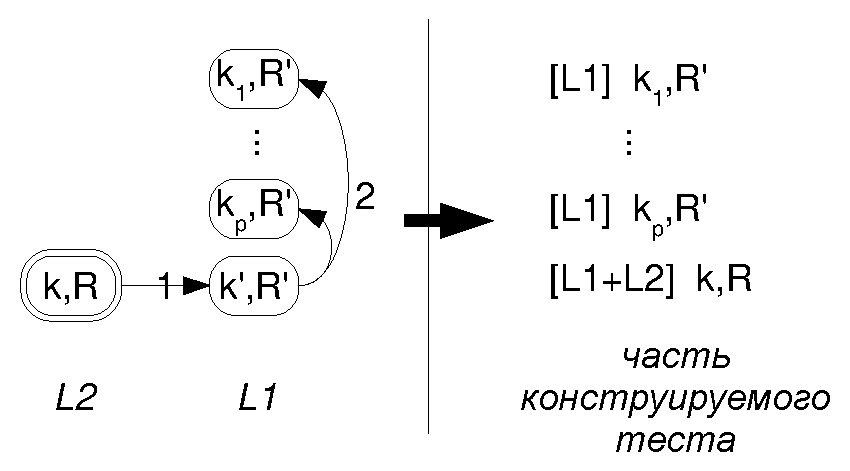
\includegraphics[width=0.6\textwidth]{2.theor/L1L2}
\caption{Конструирование обращения в кэш-память второго уровня вместе с
обращениями в кэш-память первого уровня}\label{fig:L1L2}
\end{figure}

Итак, по ключу и региону для кэш-памяти первого уровня
инструкция составляется по только что приведенной схеме. С одним лишь
уточнением, что адрес в этой инструкции должен быть таким, что при обращении по нему кэш-память
второго уровня не задействована. Теперь разберемся с последовательностью ключей
и регионов для кэш-памяти второго уровня. Рисунок~\ref{fig:L1L2} схематически
показывает, какие дополнительные инструкции надо построить для произвольного
обращения по ключу $k$ в регион $R$ кэш-памяти второго уровня. А именно, ключу
$k$ в регионе $R$ соответствует некоторый адрес, этому же адресу соответствуют и
некоторый ключ $k'$ в регионе $R'$ кэш-памяти первого уровня (стрелка с цифрой
1). Но надо еще обеспечить отсутствие этого ключа, иначе обращения в кэш-память
второго уровня не будет. Для этого надо сгенерировать небольшую
последовательность произвольных различных и не равных $k'$ ключей $k_1, k_2,
\dots, k_p$ и обратиться по ним в регион $R'$ кэш-памяти первого уровня без
затрагивания кэш-памяти второго уровня (значение числа $p$ зависит от стратегии
вытеснения).

%Рассмотрим один часто встречающийся случай кэширующих буферов,
%инициализация которого может вызывать трудности. Речь идет о
%кэш-памяти второго уровня. Зачастую кэш-память второго уровня не
%может быть инициализирована отдельно от остальных подсистем
%микропроцессора, обычно оно связано с изменением кэш-памяти первого
%уровня. Это создает дополнительные сложности при формулировании
%ограничений методом зеркальной генерации, поскольку инициализирующая
%последовательность должна подготавливать сразу два кэширующих буфера
%одновременно -- кэш-память первого уровня и кэш-память второго
%уровня. Кроме того, зачастую кэш-память второго уровня является
%совместной для хранения в ней данных и инструкций. Поэтому на
%инициализацию кэш-памяти второго уровня влияют и сами
%инициализирующие инструкции, и даже адрес расположения тестовой
%программы в памяти (от него зависит виртуальный адрес инструкций, а
%значит теги и индексы при обращении к кэш-памяти инструкций).
%
%Если принять дополнительное требование (и оно даст решение), что в
%кэш-памяти второго уровня наборы, используемые для доступа к
%инструкциям, не пересекаются с наборами, используемыми для доступа к
%данным, то генерируемые ограничения упрощаются (кэширование
%инструкций можно вообще не учитывать). С точки зрения зеркальной
%генерации это означает, что надо сформулировать требования на
%инициализирующую последовательность. Напомню, что одним из ключевых
%требований является произвольность начального состояния
%(содержимого) кэш-памяти.
%
%Предположим, что обращение к кэш-памяти второго уровня
%осуществляется при кэш-промахе в кэш-памяти первого уровня и
%кэш-память не является virtually indexed virtually
%tagged~\cite{HennessyPatterson3rd}. Для составления ограничений с
%использованием функций полезности необходимо знать, которые
%инструкции среди инициализирующей последовательности действительно
%обращаются в кэш-память второго уровня (иными словами, в каких
%инструкциях среди инициализирующей последовательности происходит
%кэш-промах при обращении к кэш-памяти первого уровня). Возможным
%решением было бы перебирать всевозможные распределения тестовых
%ситуаций в кэш-памяти первого уровня на элементах инициализирующей
%последовательности (с предварительной подготовкой этих тестовых
%ситуаций). Однако следующая лемма~\ref{special_initialization_L2}
%показывает, что для любого такого произвольного распределения
%тестовых ситуаций в кэш-памяти первого уровня существует решение со
%специальным распределением тестовых ситуаций. Это позволяет
%перебирать только такие специальные распределения тестовых ситуаций
%в кэш-памяти первого уровня. При этом вычислительная сложность
%процедуры поиска инициализирующей последовательности, дающей
%решение, изменяется от экспоненциальной от длины тестового шаблона к
%полиномиальной, что показывает лемма~\ref{max_k_h} (ее доказательство
%приведено в приложении~\ref{proofs}):
%\begin{lemma}[Верхняя оценка длины специальной инициализирующей
%последовательности для стратегии вытеснения \LRU]\label{max_k_h}\MaxUpperBoundLRU
%\end{lemma}
%\begin{sld}
%$$m = O(n)$$ где $m$ --- длина специальной инициализирующей
%последовательности, $n$ -- количество инструкций тестового шаблона.
%\end{sld}
%
%Для получения инициализирующей программы минимальной длины, можно
%применять сначала двоичный поиск суммы $k+h$ с применением
%дальнейшего поиска допустимых значений $k$ и $h$. 
%%%
%%%% !Mode:: "TeX:UTF-8"
\chapter{Программная реализация}

%%\begin{abstract}
%{\textit Небольшое отступление о множествах, функциях полезности и
%прагматике. Уравнения с множествами (и вообще использование
%множеств) взялись из попытки компактного описания
%последовательностей кэш-промахов и кэш-попаданий (интересно, как с
%этой проблемой борется Genesys-Pro). Компактность удалось достичь.
%Была надежда, что эта компактная форма записи даст и неплохой
%алгоритм разрешения (с глубоким использованием особенностей операций
%над множествами). Однако на реальных данных формула, выписанная на
%множествах, получалась очень большой длины (пропорционально размеру
%самой кэш-памяти). К счастью, появилась иная идея описания
%кэш-попаданий и кэш-промахов в ограничениях -- использование функций
%полезности (т.е. ограничения вида <<тегсет еще не вытеснен/тегсет
%уже вытеснен>>). В общем случае использование функций полезности не
%дает выигрыша, но при совместном рассмотрении кэш-памяти и TLB, т.е.
%при возможности использовать пересечение хранящихся в них данных,
%удается выписать ограничения компактного размера с использованием
%функций полезности.
%
%Таким образом, в работе представлены два новых способа записи
%тестовых ситуаций в кэш-памяти с использованием ограничений --
%уравнения на множества тегов и уравнения с функциями полезности.}
%%\end{abstract}

\section{Структура генератора тестовых программ}

В главе описывается система генерации тестовых программ на основе
тестовых шаблонов. Входными данными системы являются:
\begin{itemize}
\item тестовый шаблон;
\item описания тестовых ситуаций;
\item начальное состояние микропроцессора;
\item дополнительные параметры конфигурации.
\end{itemize}

Выходом системы является тестовая программа, удовлетворяющая
тестовому шаблону с учетом данных описаний тестовых ситуаций и
начального значения микропроцессора. Ядром системы является
\emph{генератор ограничений} (см. рис.~\ref{structure}). Ограничения
разрешаются другим компонентом системы -- \emph{решателем
ограничений}. Модель, построенную решателем ограничений, анализирует
\emph{генератор инструкций тестовой программы}, с целью построить
готовую тестовую программу.

\begin{figure}[h] \center
  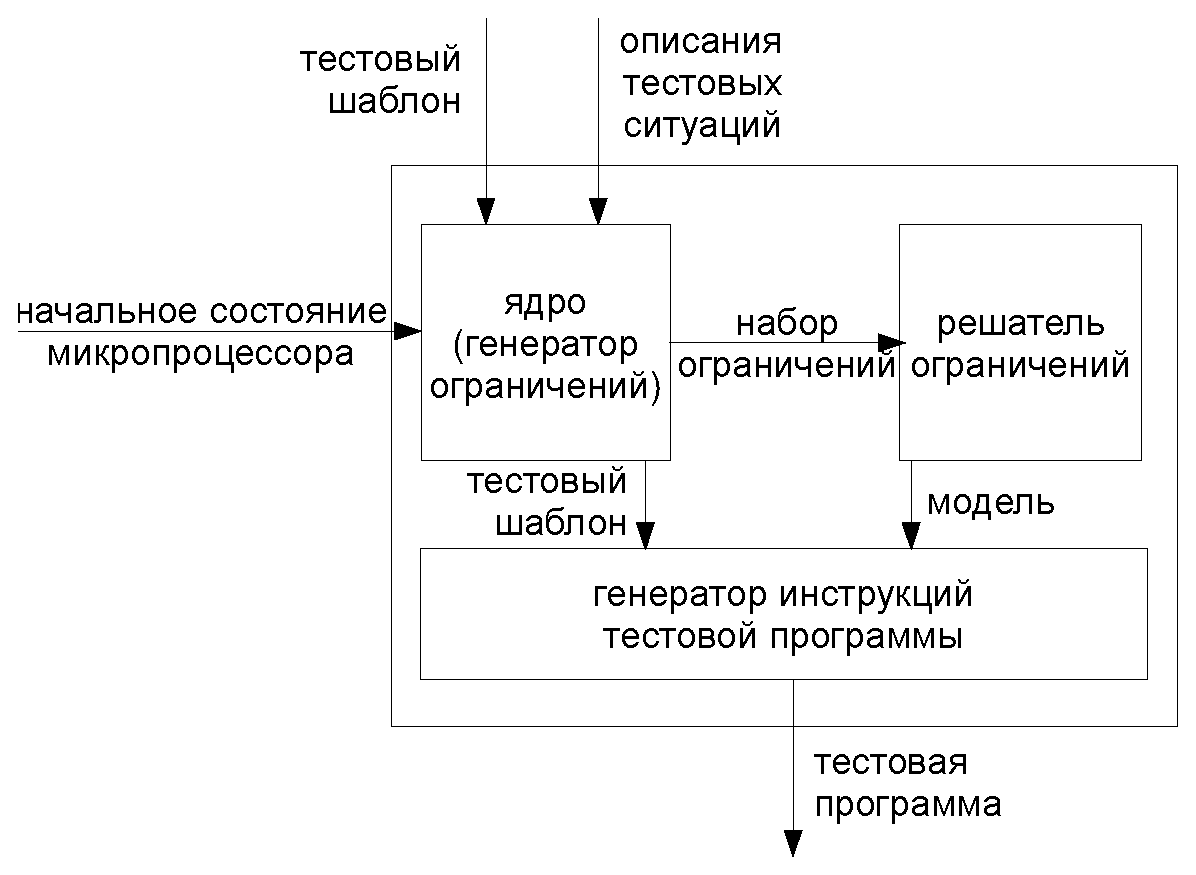
\includegraphics[width=0.8\textwidth]{3.impl/structure}\\
  \caption{Структура системы генерации тестовых программ}\label{structure}
\end{figure}

На рис.~\ref{comparison_genesyspro} показано сравнение предлагаемого
генератора тестовых программ с известным генератором
Genesys-Pro~\cite{GenesysPro}. Оба генератора получают на вход
тестовый шаблон, а на выходе у них тестовые программы.

Genesys-Pro на вход требует architectural model и testing knowledge
-- первая дает по сути эталонный симулятор микропроцессора (задает
операционную семантику инструкций и модель состояния
микропроцессора), а второй описывает эвристики выбора аргументов для
инструкции. Genesys-Pro чётко разделяет свойства аргументов
инструкции и свойства результата инструкции, соотношение между ними
задается не с помощью ограничений (т.е. не декларативным способом),
а в виде алгоритма (т.е. императивным способом). Genesys-Pro не
предполагает систематического описания семантики инструкций,
выделения ветвей их функциональности, описания программных
контрактов инструкций. Симулятор нужен для построения модельного
состояния микропроцессора после исполнения очередной сгенерированной
инструкции, а эвристики выбора аргументов составляют основу тех
ограничений, которые описывают значения аргументов очередной
инструкции.

Другой особенностью Genesys-Pro является то, что поддерживаемые им
тестовые шаблоны зачастую не фиксируют последовательность инструкций
(это позволяет строить более простые ограничения, потому как
генерируемая последовательность инструкций может по ходу генерации
подстраиваться под уже сгенерированные инструкции со
сгенерированными значениями аргументов, под состояние
микропроцессора, в которое привели сгенерированные инструкции).

Выразительный язык Genesys-Pro для описания ограничений однако
содержит такие нетривиальные конструкции, как явное использование
элементов массивов данных, что требует для разрешения продвинутый
решатель CSP, в том числе и заточенный под особенности генерации
тестовых данных для тестовых шаблонов (как минимум такие ограничения
могут включать битовые операции). Подобный решатель был разработан в
IBM для инструмента Genesys-Pro~\cite{GenesysSolver}. Однако
создание такого решателя -- отдельное сложное исследование, которое
не входило в цели данного исследования. В данной работе было принято
решение использовать доступные существующие решатели (не обязательно
CSP) и сосредоточиться на упрощении генерируемых ограничений для
некоторых частных случаев архитектур.

\begin{figure}[h]
\parbox{0.5\textwidth}{ \centering
  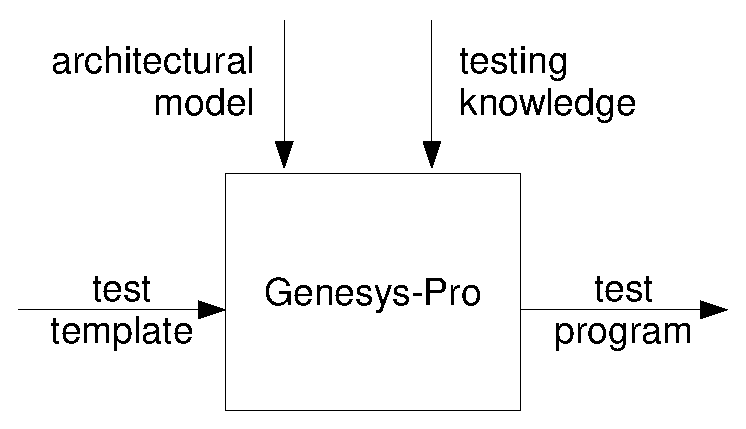
\includegraphics[width=0.45\textwidth]{3.impl/genesys-pro}
} \vline
\parbox{0.5\textwidth}{ \centering
  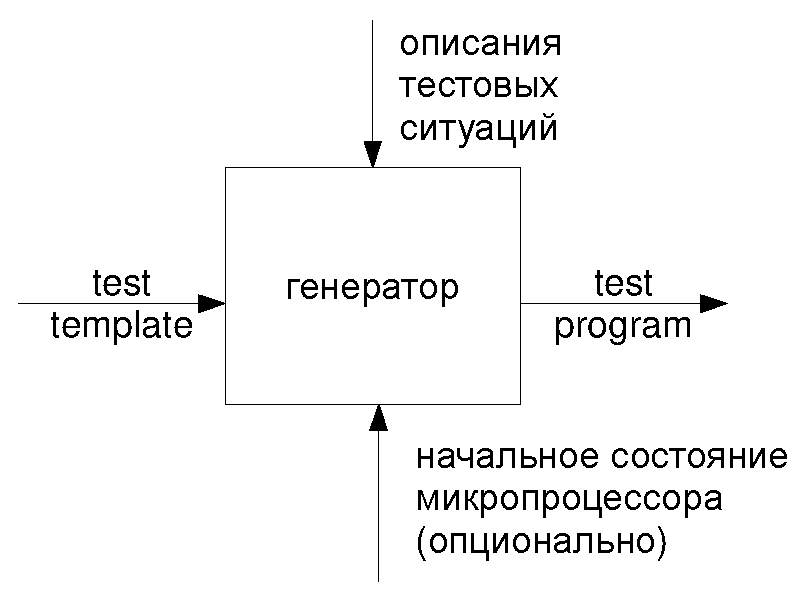
\includegraphics[width=0.45\textwidth]{3.impl/mygen}
}
\caption{Сравнение с Genesys-Pro}\label{comparison_genesyspro}
\end{figure}

В отличие от Genesys-Pro в предлагаемом инструменте описание
семантики инструкций задается в едином виде -- в виде описаний
тестовых ситуаций~\cite{my_syrcose_2008, my_isp_2008}. Каждая
тестовая ситуация описывает не только ограничение на свои аргументы,
но и результат исполнения инструкции \emph{при данном ограничении на
аргументы} инструкции декларативным образом. В функции, которую
реализует инструкция, выделяются отдельные \emph{ветви
функциональности}, ситуации различного поведения инструкций, каждая
ветвь функциональности становится отдельной тестовой ситуацией.
Например, инструкция целочисленного сложения ADD может быть
исполнена либо точно, либо с возникновением переполнения. Поэтому у
этой инструкции можно выделить 2 ветви функциональности (точное
исполнение и исполнение с переполнением), каждая ветвь дает свою
тестовую ситуацию. Кроме того, предлагаемый генератор дает
возможность указать начальное состояние микропроцессора, которое
будет эффективно использовано при построении тестовой программы.
Последовательность инструкций фиксирована и задается в тестовом
шаблоне.

Описания тестовых ситуаций можно составлять по следующей схеме:
\begin{enumerate}
\item выделить тестируемые инструкции;
\item найти описание семантики выбранных инструкций (обычно оно
входит в документацию по тестируемой архитектуре);
\item для каждой инструкции выделить:
    \begin{itemize}
    \item аргументы: имена и битовые длины;
    \item предусловие (ограничение на значения аргументов
    инструкции, при которых она может быть результативно исполнена);
    \item ветви функциональности инструкции (ситуации различного
    поведения инструкции);
    \end{itemize}
\item для каждой ветви функциональности составить описание тестовой
ситуации, поместив туда объявления аргументов, предусловие и
операторы, описывающие поведение инструкции на данной ветви
функциональности, т.е. вычисление выходного значения инструкции или
создание условий возникновения исключительной ситуации.
\end{enumerate}

Раздел~\ref{tesla} содержит описание предлагаемого языка описания
тестовых шаблонов и тестовых ситуаций, пригодный для описания
инструкций арифметической, логической подсистем, подсистемы
обращения к памяти, инструкции переходов.

\section{Описание тестовых шаблонов}\label{tesla}

Описание тестового шаблона состоит из следующих секций:
\begin{enumerate}
\item \emph{заголовок шаблона}: объявление регистров и констант;
\item \emph{тело шаблона}: инструкции и ограничения тестового
шаблона.
\end{enumerate}

Заголовок шаблона должен содержать объявления всех задействованных в
тестовом шаблоне регистров (для каждого регистра указывается его имя
и битовая длина) и констант (или по-другому, <<непосредственных
значений>> -- для каждой константы так же указывается ее имя и
битовая длина). Регистр может использоваться в качестве
аргумента-результата инструкции, константа не может использоваться в
качестве аргумента-результата инструкции. Регистры и константы
сохраняют свою битовую длину на протяжении всего тестового шаблона.
Генератор ограничений трактует регистр как переменную со значением и
генерирует начальное значение такой переменной, при которой
выполнены все заявленные в тестовом шаблоне тестовые ситуации.
Обычно для инициализации регистра достаточно одной-двух инструкций
(это зависит от количества бит, которое может изменить одна
инструкция). Константа трактуется как значение, которое не меняется.
Для нее тоже генерируется значение и при составлении тестовой
программы оно вставляется непосредственно на место аргумента
инструкций.

Пример объявления регистра и константы: {\small \begin{verbatim}
    <register id="z" length="64" />
    <constant id="c" length="16" />
\end{verbatim}}

Тело тестового шаблона состоит из описаний инструкций и ограничений.
Для инструкции необходимо указать:
\begin{itemize}
\item имя инструкции;
\item аргументы инструкции (объявленные ранее регистры или
константы);
\item внешние переменные инструкции;
\item тестовую ситуацию.
\end{itemize}

Тестовые ситуации на косвенные обращения не рассматриваются, поэтому
в описания тестовых шаблонов не включены механизмы описания
косвенных обращений.

\emph{Механизм внешних переменных} инструкции позволяет
формулировать ограничения на локальные переменные, определенные в
разных тестовых ситуациях. При объявлении новой локальной переменной
кроме имени можно указать идентификатор (имя надо указывать
обязательно, а идентификатор -- необязательно). Все идентификаторы
внутри тестовой ситуации должны быть уникальными. Это может быть
виртуальный адрес, физический адрес, некое внутреннее выражение.
Если тестовая ситуация является составной, то все тестовые ситуации
должны определять выносимые на уровень тестового шаблона
идентификаторы. На уровне тестового шаблона идентификатору ставится
в соответствие некоторое новое уникальное внутри шаблона имя,
которое можно использовать наравне с другими переменными (регистрами
или константами).

Тестовая ситуация описывает некоторое поведение инструкции. Обычно
можно выделить два типа поведений инструкции: существенное
исполнение (вычисление значения, осуществление взаимодействия) и
генерация исключения. При существенном исполнении тестовая ситуация
описывает предусловие инструкции и набор условий и вычислений,
определяющих данное поведение инструкции. При исполнении с
генерацией исключения описывается предусловие инструкции и набор
условий и вычислений, приводящих к возникновению исключения. Само
возникновение исключения, как оператор, не описывается.

Тестовая ситуация состоит из набора \emph{ветвей} -- простейших
поведений инструкции. Ветви могут \emph{комбинироваться} в
дизъюнкции и конъюнкции. Дизъюнкция ветвей (или их комбинаций)
означает, что в данный момент инструкция может себя вести согласно
хотя бы одной из ветвей. Конъюнкция ветвей (или их комбинаций)
означает, что в данный момент инструкция может себя вести согласно
всем ветвям одновременно. Объединенные в конъюнкцию ветви не могут
иметь существенное исполнение.

Пример тестовой ситуации ветви: {\small
\begin{verbatim}
        <situation>
            <branch name="overflow" />
        </situation>
\end{verbatim}}

Для ветви указывается имя. Оно используется при поиске
соответствующего файла с описанием этой тестовой ситуации. Поиск
производится на основе имени тестовой ситуации и имени инструкции,
для которой она указана.

Пример тестовой ситуации, включающей комбинацию ветвей: {\small
\begin{verbatim}
        <situation>
            <or>
                <and>
                    <branch name="overflow" />
                    <branch name="normal" />
                </and>
                <branch name="zero" />
            </or>
        </situation>
\end{verbatim}}

Эту комбинацию ветвей можно прочесть следующим образом: \emph{данная
инструкция должна себя вести как overflow с normal или как zero}.

В описаниях тестовых ситуациях могут быть фиксированы обращения к
различным подсистемам микропроцессора. Указание тестовой ситуации в
шаблоне может фиксировать и тестовую ситуацию на эти обращения (а
для полных тестовых шаблонов оно \emph{должно} фиксировать тестовую
ситуацию на эти обращения). Среди подсистем можно выделить различные
кэширующие буферы (например, уровни кэш-памяти, TLB, другие
подсистемы). Содержимое секции тестовых ситуаций обращений к
подсистемам определяется архитектурой тестируемого микропроцессора.
Например, оно может быть следующим: {\small
\begin{verbatim}
    <situation>
            ...
            <access>
                <cache level="1" type="DATA" id="miss" />
                <cache level="2" type="DATA" id="miss" />
                <cache level="3" type="DATA" id="hit" />
                <tlb  id="invalid">
                    <microtlb type="DATA" id="miss" />
                </tlb>
            </access>
    </situation>
\end{verbatim}}

Это описание говорит о том, что при исполнении данной инструкции в
кэш-памяти данных первого и второго уровней должен быть кэш-промах,
а в кэш-памяти данных третьего уровня -- кэш-попадание; в TLB должна
произойти тестовая ситуация invalid, а в MicroTLB данных -- промах.
Интерпретация терминов \texttt{cache, tlb, microtlb, miss, hit,
invalid} заложена в части генератора ограничений, ответственного за
тестируемую архитектуру.

Кроме инструкций тестовый шаблон может содержать <<допущения>>
(assume) -- некоторые ограничения на текущее состояние
микропроцессора и введенные внешние переменные. Можно выделить
следующие основные применения этих ограничений:
\begin{enumerate}
\item задание зависимостей на адреса разных инструкций (например, у
двух инструкций одинаковые физические адреса при разных виртуальных
адресах -- одна инструкция определяет свои виртуальный и физический
адрес, другая инструкция делает то же, а ограничение фиксирует связь
значений этих четырех переменных);
\item задание ветви в графе потока управления: при тестировании
инструкций перехода с некоторым сравнением вместо их
непосредственного описания предлагается описывать конкретные
результаты сравнений (истинно это сравнение в данный момент или
ложно); тестовый шаблон не позволяет описывать разветвленные потоки
управления, разрешается описывать лишь последовательности
инструкций, поэтому такие дополнительные ограничения позволяют
описать в тестовом шаблоне один из путей в графе потока управления и
сгенерировать для этого пути свою тестовую программу.
\end{enumerate}

Описание ограничения, как и описание тестовой ситуации, может
состоять из указания ветви или их комбинаций. Пример: {\small
\begin{verbatim}
    <assume>
        <or>
            <and>
                <branch name="ff1" />
                <branch name="ff2" />
                <branch name="ff3" />
            </and>
            <branch name="ff4" />
        </or>
    </assume>
\end{verbatim}}

Пример описания тестового шаблона целиком: {\small
\begin{verbatim}
  <template>
    <register id="x" length="64" />
    <register id="y" length="64" />
    <register id="z" length="64" />
    <constant id="c" length="16" />

    <instruction name="ADD">
        <argument name="x" />
        <argument name="y" />
        <argument name="z" />
        <external name="v1" id="virtual" />
        <external name="p1" id="phys" />
        <situation>
            <or>
                <and>
                    <branch name="overflow" />
                    <branch name="normal" />
                </and>
                <branch name="zero" />
            </or>

            <access>
                <cache level="1" type="DATA" id="miss" />
                <cache level="2" type="DATA" id="miss" />
                <cache level="3" type="DATA" id="hit" />
                <tlb  id="invalid">
                    <microtlb type="DATA" id="miss"></microtlb>
                </tlb>
            </access>

        </situation>
    </instruction>

    <assume>
        <or>
            <and>
                <branch name="ff1" />
                <branch name="ff2" />
                <branch name="ff3" />
            </and>
            <branch name="ff4" />
        </or>
    </assume>
</template>
\end{verbatim}
 }

\section{Описание тестовых ситуаций}

Описание тестовой ситуации состоит из следующих секций:
\begin{enumerate}
\item \emph{заголовок тестовой ситуации}: объявление аргументов инструкции;
\item \emph{тело тестовой ситуации}: последовательность операторов.
\end{enumerate}

Заголовок тестовой ситуации должен содержать объявления всех
аргументов инструкции. Для каждого аргумента указывается его имя
(локальное внутри данной тестовой ситуации), статус <<только для
чтения/результат>> и битовая длина. Последовательность аргументов
тестовой ситуации должна совпадать с последовательностью аргументов
инструкции с точностью до переименования. Иными словами, первый
аргумент тестовой ситуации должен обозначать первый аргумент
инструкции (их битовые длины должны совпадать), второй аргумент
тестовой ситуации -- второй аргумент инструкции и так далее.
Аргументы, помеченные статусом <<только для чтения>> не могут менять
свое значение во время всей тестовой ситуации. Аргументы, помеченные
статусом <<результат>> обязаны получить значение в данной
инструкции. Тестовая ситуация может иметь произвольное количество
аргументов обоих статусов в произвольном порядке. Статус <<только
для чтения>> позволяет передать в качестве аргументов инструкции
одинаковые переменные (одинаковые регистры или константы). Однако
все аргументы инструкции, соответствующие аргументам тестовой
ситуации со статусом <<результат>>, должны иметь разные имена (они
могут быть среди аргументов со статусом <<только для чтения>>).

Пример: {\small
\begin{verbatim}
 <argument name="rt" state="result" length="64"/>
 <argument name="base" state="readonly" length="64"/>
 <argument name="offset" state="readonly" length="16"/>
\end{verbatim}}

Тело тестовой ситуации состоит из последовательности операторов трех
видов:
\begin{itemize}
  \item оператор \texttt{let} -- объявление новой локальной
  переменной вместе с ее инициализацией;
  \item оператор \texttt{assume} -- фиксация некоторого ограничения
  (<<допущения>>) на значения переменных;
  \item оператор \texttt{procedure} -- вызов процедуры (ее семантика
    не задается в описании тестовой ситуации).
\end{itemize}

Тестовая ситуация по своей сути является ветвью функциональности
инструкции. Поэтому ее описание содержит лишь последовательность
операторов, условные операторы и операторы цикла отсутствуют.

Оператор \texttt{let} объявляет новую переменную и инициализирует ее
результатом вычисления некоторого выражения. Оператор может
содержать указание имени переменной (оно должно быть новым)
\emph{или} указание идентификатора новой переменной (все
идентификаторы внутри тестовой ситуации должны быть разными;
идентификатор может совпадать с именем этой или любой другой
переменной). Безымянные операторы \texttt{let} позволяют задать
идентификатор существующей переменной.

Тело оператора содержит выражение, результат вычисления которого
станет значением объявляемой переменной. Выражение может содержать
следующие операции:
\begin{itemize}
  \item переменные (\texttt{var}) и константы (\texttt{constant});
  допустимы только неотрицательные константы, у каждой константы
  должна быть указана битовая длина;
  \item битовые операции: выделение бита с заданными номером (\texttt{bit}),
  выделение непрерывной последовательности бит с заданными границами
  (\texttt{bits}), битовая конкатенация (\texttt{concat}), битовая
  степень (\texttt{power});
  \item арифметические операции: сложение (\texttt{sum}), вычитание
  (\texttt{sub}); операции проводятся по модулю экспоненты битовой
  длины аргументов.
\end{itemize}
Производится строгая <<проверка типов>>, т.е. битовых длин
аргументов операций. Например, сложению подвергаются только
выражения с одинаковыми битовыми длинами. В частности это позволяет
автоматически вычислить битовую длину объявляемой переменной.

Пример: {\small
\begin{verbatim}
<let name="vAddr" id="virtual">
    <sum>
        <sign_extend size="64"><var>offset</var></sign_extend>
        <var>base</var>
    </sum>
</let>
\end{verbatim}}

Оператор \texttt{assume} позволяет указать ограничение, справедливое
в некоторый момент на значениях аргументов тестовой ситуации и
локальных переменных. Выражения объединяются с помощью отношений
сравнения. Пример: {\small
\begin{verbatim}
    <assume>
        <eq>
            <bits end="1" start="0"><var>vAddr</var></bits>
            <constant length="2">0</constant>
        </eq>
    </assume>
\end{verbatim}}

Оператор \texttt{procedure} позволяет указать более сложное
действие, в котором могут участвовать различные подсистемы
микропроцессора. Семантика процедур не фиксируется при описании
тестовой ситуации. Аргументы, наоборот, фиксируются. Каждый аргумент
может иметь идентификатор (это позволяет располагать аргументы в
произвольном порядке, указывая семантику каждого аргумента с помощью
идентификатора). Тело аргумента может быть следующих типов:
\begin{itemize}
  \item выражение на определенные к моменту вызова процедуры
  переменные; выражение задается с использованием того же
  синтаксиса, что и в операторе \texttt{let};
  \item новая переменная (\texttt{new});
  \item символьная константа.
\end{itemize}

Набор допустимых процедур и идентификаторов их аргументов задается
генератором ограничений.

Пример: {\small
\begin{verbatim}
<procedure name="AddressTranslation">
        <argument id="physical"><new length="64">pAddr</argument>
        <argument id="virtual"><var>vAddr</var></argument>
        <argument id="points_to">DATA</argument>
        <argument id="points_for">LOAD</argument>
</procedure>
\end{verbatim}}

Пример описания тестовой ситуации целиком: {\small
\begin{verbatim}
<situation>
    <argument name="rt" state="result" length="64" />
    <argument name="base" state="readonly" length="64" />
    <argument name="offset" state="readonly" length="16" />

    <let name="vAddr" id="virtual">
        <sum>
            <sign_extend size="64"><var>offset</var></sign_extend>
            <var>base</var>
        </sum>
    </let>

    <assume>
        <eq>
            <bits end="1" start="0"><var>vAddr</var></bits>
            <constant length="2">0</constant>
        </eq>
    </assume>

    <procedure name="AddressTranslation">
        <argument id="physical"><new length="64">pAddr</argument>
        <argument id="virtual"><var>vAddr</var></argument>
        <argument id="points_to">DATA</argument>
        <argument id="points_for">LOAD</argument>
    </procedure>

    <let id="physical"><var>pAddr</var></let>

    <let name="dwByteOffset">
        <bits end="2" start="0"><var>vAddr</var></bits>
    </let>

    <!-- dwByteOffset can be changed
         according to BigEndian/LittleEndian -->

    <procedure name="LoadMemory">
        <argument id="data"><new length="64">memdoubleword</argument>
        <argument id="size">WORD</argument>
        <argument id="physical"><var>pAddr</var></argument>
        <argument id="virtual"><var>vAddr</var></argument>
        <argument id="points_to">DATA</argument>
    </procedure>

    <procedure name="BytesSelect">
        <argument id="type">WORD</argument>
        <argument id="from"><new length="32">data</argument>
        <argument id="content"><var>memdoubleword</var></arument>
        <argument id="index"><var>dwByteOffset</var></argument>
    </procedure>

    <assume>
        <eq>
            <var>rt</var>
            <sign_extend size="64"><var>data</var></sign_extend>
        </eq>
    </assume>
</situation>
\end{verbatim}}

\section{Генератор ограничений (ядро)}

Генератор ограничений имеет модульную структуру (см.
рис.~\ref{generator})~\cite{my_lomonosov_2009, my_miet_2009}. В его
составе есть модуль, ответственный за генерацию ограничений для
общих механизмов описания архитектур микропроцессоров, такие как
работа с регистрами, работа с последовательностью инструкций, работа
с локальными переменными в тестовых ситуаций, и модуль, специфичный
для тестируемой архитектуры (он содержит алгоритмы генерации
ограничений для таких механизмов, как трансляция адресов, как
кэширование).

\begin{figure}[h] \center
  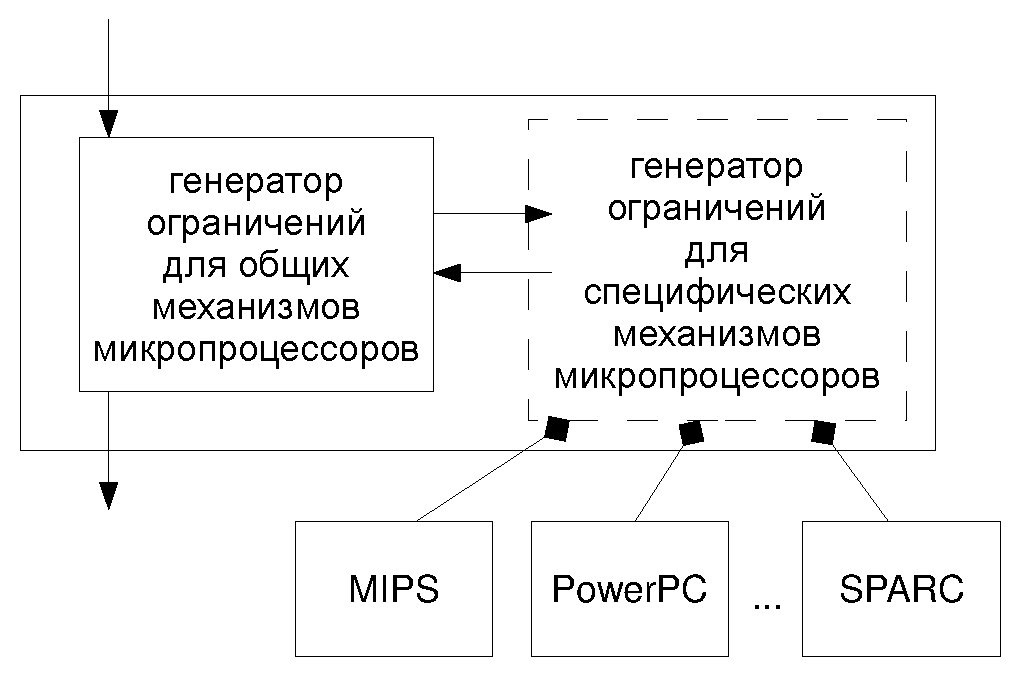
\includegraphics[width=0.5\textwidth]{3.impl/generator}\\
  \caption{Структура генератора ограничений}\label{generator}
\end{figure}

Генерация ограничений производится последовательно для каждой
инструкции тестового шаблона. Однако разрешение ограничений может
происходить быстрее при некотором порядке ограничений, это можно
учесть при генерации ограничений.

%%%
%%%\chapter{���������}

%����������� ������������: ���������� �������, ��� �������, �����
%��������� (���������� ��������� ������, ����������� �����)
%
%������� ���� ��������� �������, �������� ����� ����, ������������
%���������� ������� ������; ������� ���� �� � ������
%���������.....�������, ��� ���� ������, ����� ������������� �
%��������� ������ - ���� ������������� (��� ��������) ������
%������������ -- �������������� ������, ��������� ����� �����������,
%��������� ��������, � ��������� �� ������� ������� ����������
%�������-��. ���� �������� ��� ��� �������� � ���� ����������:
%������������ (+ ����. �� �������) , ������� ������������ (����� �� �
%���� ������ ���� ������) ( ��������, "� 6 �� 8 ������� �������
%������, � � ��������� - ������������"), (���� ������ ��������
%��������� ��������� ��� ������� �������, �� ����� ���� ����������,
%������� � ����� ������ ������� ���������������, ������� � �������,
%����� ���� �� � �� ���������!) ������������ (��� ������ ����� �����
%���� ������ �������, �� ����� ����� ���������� -- ������ ������
%��������� �������) ---  ����������� ������������ (����� ����������
%������), ������� � ������������ (���-�� ��������������� ������).
%��������, ��� ��������� �������� ������������ ������ ����-����,
%���-�� ������ �����-��, � ��� ������ ������ ���-��, � ���-�� ������
%������ �� �������. � ����� �� ��������� ������ ���� ���������! ��� �
%����� ����������� �����������, ������� ����������� ������.
%
%������������  �������  ������������

����� �������� ���������� ���������� �������� �������� �� ��������
�������� ��� ���������� ���������������. ��� ����� ���� ���������
��������� ������������������� �����:
\begin{enumerate}
  \item ���������� ����� MMU ��������������� (��������� ����������
  ������� � ������, ����������� ����������� �������) -- ��� �����
  ���� ������������ � ������������� �� MMU ���������������;
  \item\label{procedures_choose} ����� �������� ��� ����� ��������
  �������� �������� -- ���
  ����� ���� ������������ � ������������� �� ������� ������
  ���������������;
  \item ��������� ���������� �����������, ��������������
  ������������������ �������� �������� � ���������� ������� -- ���
  ����� ����� ��������� ������ ���������� � ���������� ���������
  �����������;
  \item ��������� ���������� ����������� ��� ��������, ��������� ��
  ����~\ref{procedures_choose} -- ����� ������������� ������������ �
  ������������� �� ���������������;
  \item ���������� �������� �������� �������� ��� ����������
  ��������������� -- ��� ����� ���� ������������ � �������������
  �� ������� ������ ���������������;
  \item ��������� ����������� ������ �������� � ���������� ��������
  ���������;
  \item ����������� ���������� ������� ���������� � ������ ����� (�
  �������������� �������� ���������� ���������� �����������, ������������
  �� ����������� ���������������);
  \item ������ ���������� ����������� � ��������� �����������.
\end{enumerate}


\section{��������� ����������� ��� ����������� MIPS}

\begin{utv}
��� ����������� MIPS �������� ���������� ���������� �������
��������� �����������, ����������� � �����������, ��� ���������
�������� �������� �� �������� ��������; ������ ������� ����������
��� ������� �������� ��������� MMU ���������������� �����������
MIPS.
\end{utv}

���������� ���������� ���������� ��������� � ������ �
��������������� ����������� MIPS~\cite{mips64_III}. MMU �
���������������� MIPS �������� � ����  (��������������
�������������� ��������� ��� ��������������� MIPS R10000 -- ��.
���.~\ref{mips_mmu_scheme}):
\begin{itemize}
  \item \emph{���-������ ������ ������� ������ (D-Cache-1)}:  virtually
indexed physically tagged, ������ 32 ���������, ������ ������
���-������ 32 �����, �������-������������� ���-������,
��������������� ����� 2, ��������� ���������� \LRU;
  \item \emph{���-������ ������� ������ (Cache-2)}: ������ �� 512 �������� �� 16
��������~\cite{shnitman}, ��������� ���������� LRU;
  \item \emph{���������� ����� TLB (D-TLB)}: ���������
  �������������, ������ 4 ������;
  \item \emph{������������ TLB (Joint-TLB)}: ������ 48 �����,
  ������ ������������ ������ 64 ����.
\end{itemize}
����� �������, �������� �������� ��� ������ ����������� -- �������
������ ����������� ���-������.

���������� ����� ��������� �������� �������� �:
\begin{itemize}
  \item ���-������ ������ ������� ������, ������� � ������� �������;
  \item ���-������ ������ TLB (D-TLB).
\end{itemize}

���������� ��������� �������� �� ������� TLB--���-������, ��� ���
���������� �� TLB ����� ����������� ����� (pfn) ���������� �������
����� ������� ����������� ������ (��.���.~\ref{mips_mmu_scheme} --
��������� ���������� ����� ���������� ���������� ���������,
��������� ���������� ���������� ����������� ������ �������).

\begin{figure}[h] \center
  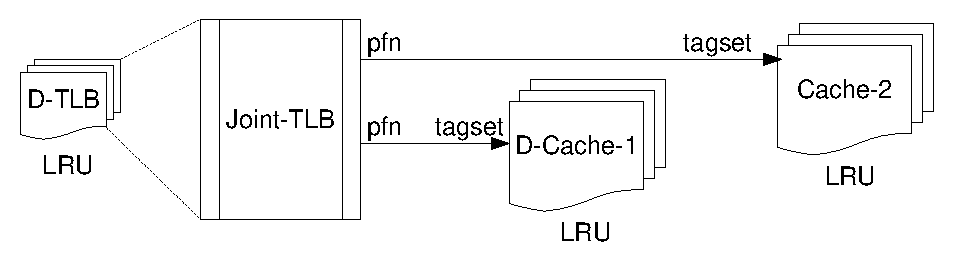
\includegraphics[width=0.8\textwidth]{4.analysis/mips}\\
  \caption{����� MMU ��������������� MIPS}\label{mips_mmu_scheme}
\end{figure}

�� ����� ���������� ���������� �������� ��������:
\begin{enumerate}
  \item\label{step_mmu} ��������� MMU ���������, ��� ����� �������� ������������ �
  ������������� �� ����������� ���������������~\cite{mips64_III},
  ��� ������ 1 ��������-����;
  \item\label{step_procedures}
  �� ������ ������� ������� ������ ����������� MIPS~\cite{mips64_II}
  ���� �������� ��������� ��������� ��� �������� ��������
  ��������:\\
  AddressTranslation, LoadMemory, StoreMemory, BytesSelect,
  BytesExpand -- �� ��� ���� 1 ��������-����;
  \item � ���������� ����������� ��� ����������� ���������� �����
  ��������� ����������� ��� ���������� �������������� ��������� �
  ���������-���������� ����� ��������� ����������� ��� ���������
  ��������� -- �� ��� ���� � ������ ������� 5 ��������-����;
  \item ��� ��������� AddressTranslation � ���� ����������� ����
  �������� ������ ����������� ������ (���� ��������� � ������
  �������� ����������� ������ -- ���������� ��� ������������,
  ������������ ��� ��������������), ��� ��������� LoadMemory � ����
  ����������� ���� �������� ����������� ���������� ������� �
  ��������� �� �������� ������ ������ (��.
  �.~\ref{module_algorithm} �����������), ��� �������� BytesSelect �
  BytesExpand ��� ������� ������� �������� ������� ��� �����������
  ������ � ������ ����� ������ ����� �������� �����, ���������
  ����������� ������ �� ������ ��� ������ � ������ -- � ������
  ������� �� ��� ���� 3 ��������-���;
  \item\label{step_testsituations}
   �� ����������� ���������� � ������������� �� ������� ������
  ����������� MIPS~\cite{mips64_II} ���� �������� 8 ����������
  (load / store --- byte / halfword / word / doubleword), � ������ ���������� ��
  2 �������� �������� (AddressError(������������� �����������
  �����) / ������ ���������� ����������), �� ���������� ��������
  �������� �������� ���� 1 ��������-����;
  \item\label{step_z3} ������������� �������� ����������� Z3~\cite{Z3}, �������
  ������� ������ � ���� ��� <<(���, ��������)>>, ����� ����
  ���������� ��������� �������� ��������� � ���������������� �������
  ���������� �������������� ���������, �� ������� ��������������
  ���������������� ���������� -- � ������ ������� �� ��� ���� 1
  ��������-����;
  \item\label{step_compose} ���� ���������� ��������� ���������� ������ ��������
  �������� �������� � ���������� ����������� ��� ����������
  \texttt{let} � \texttt{assert} � ����� ����������, �����������
  ������������������ �������� �������� � ���-������ � TLB,
  ����������� ��������� �������� �������� �������� � ������������
  ������� �������� ��������� -- �� ��� ���� 1 ��������-����.
\end{enumerate}

����� �� ���������� ���������� �������� �������� ��� MIPS ���� �����
2,5 ��������-������. ��� ���� ��� ���������� ���������� ��������
�������� ��� ������� ��������������� ����������� MIPS (�� �����
���������� ��������������� ����������� ���������� �������, ���������
����������� � ���������� �������) �������� ����� ������������
���������� ����� \ref{step_mmu}, \ref{step_procedures},
\ref{step_testsituations}, \ref{step_z3} � \ref{step_compose},
��������� ���� ����������� ����������� ������� � �������
�������������� ���������� . ��� ��������� ������� �������
����������������� � 40\% ($\frac{5 * 100\%}{13}$). ������ ��������
���������� �������� ��������� ��� ��������������� MIPS RM7000
~\cite{kamkin} ������ \_\_\_\_\_\_\_ ��������-����. ������ �
������������ ����������, ��� ��� ������� ������� ��������� ������
�������������� � ����������� ������ ��������� ��������� �����
���������� ���������� �������� �������� � \_\_\_\_\_\_\_  ���.

��� ����������� �������� ���������� �������� �������� ���
��������������� ����������� MIPS. ���� ��������� ������������ ��
��������� �������� �������� �� �������� �������� ��������. ������
����� ������������� ��� ������ � ������������� ����������� ����, ���
�����������, ����������� �� ������ ���������� ���������, �����
��������� � ����� ������� �������� ���������. � �������~\ref{exps1}
��������� ���������� ���� ������������� ��� �������� �������� ��
���� ����������. ����� �������� �������� � ����������
���������������� ������������� �� ������ ���� 240. �� ��� 15\%
������������ �������� �������� (��� ��� �� ����� ������������ ��
���� �������� ���������). ��������� 85\% �������� �������� ���������
������ �������������. ���� ������������ ��������� ���������
��������������� ���� �����: ������������ (�������� ����� � �������
���-������ ���� ������������� ��������� �������) � ��������������
(�������� ����� � ������� ���� ������� ���, ����� ��� � �������
������������ ������������ � �������� ���������� ������ ���������
TLB).

\begin{table}[h]
  \begin{tabular}{|c|c|c|c|c|}
  \hline
  \begin{tabular}{c}���\\����������\\���������\end{tabular}&
  \begin{tabular}{c}����\\�����-\\��������\\��������\\��������\end{tabular}&
  \begin{tabular}{c}����\\���������-\\������\\��������\\��������\end{tabular}&
  \begin{tabular}{c}���\\����������\\���������\end{tabular}&
  \begin{tabular}{c}�����\\�����\\���������\end{tabular}\\
  \hline \hline
  �������������� & 49~\% & 36~\% & 58~\% & 85~�. \\
  \hline
  ������������ & 32~\% & 53~\% & 38~\% & 170~�. \\
  \hline
  \end{tabular}
  \caption{������������ � ���������� ����������; $n$ =
  2}\label{exps1}
\end{table}

������������ ��������, ��� ������������� ���������� ��������� ��
������������ ��������� ������ ���� ����������� ��������� ��������
��������� ��� 35-40\% �������� �������� � ���������� �������������
�� ���������; �� �������������� ��������� ������ �����������
���������� ��������� ������� ������� 55-60\% �������� ��� ��������
��������. ����� ��� ������, ��������� ��� ������ ������� ���������
��������������� ����� ������������, � ��� ���� ����������� ��������
���������, ���������� �� ������� ��������, ����� ��� ���������������
--- ��� ����� ��������� ����������� ���������� �������� ��������� ��
������������, ��������������� ������� ���������� ���������.
���������� ������� (� ���� ��� �������) ������� ��������� ��������
��������� ��� ���� �������� ���������� ��������. �� ��� ��������
������� <<����������� ������>> ������������� ����� 220 ������.

%% ���������� n = 3 � n = 4

%% ���������� ������������ ����� ����������� ����������� �����
%% ���������������� ������������������ ��� ���������� ���������

\section{��������� ����������� ��� ����������� PowerPC}

\begin{utv}
��� ����������� PowerPC �������� ���������� ���������� �������
��������� �����������, ����������� � �����������, ��� ���������
�������� �������� �� �������� ��������; ������ ������� ����������
��� ������� �������� ��������� MMU ���������������� �����������
PowerPC.
\end{utv}

���������� ���������� ���������� ��������� � ������ �
��������������� ����������� PowerPC~\cite{shnitman}. MMU �
���������������� PowerPC �������� � ���� (��������������
�������������� ��������� ��� ��������������� PowerPC 970FX
~\cite{PowerPC970FXUserManual} -- ��.
���.~\ref{powerpc_mmu_scheme}):
\begin{itemize}
  \item \emph{���-������ ������ ������� ������ (D-Cache-1)}: ������ 32
���������, �������-������������� ���-������, ���������� ������ �����
2, ������ ������ ���-������ 128 ����, effective index real tag,
��������� ���������� \LRU;
  \item \emph{���-������ ������� ������ (Cache-2)}: ������ 512
  ��������, �������-������������� ���-������, ���������� ������
  ����� 8, ��������� ���������� LRU, ������ ������ ���-������ 128
  ����, real index real tag;
  \item \emph{���-����� TLB (D-TLB)}: �������-������������� �����,
  ���������� ������ 4, ���������� ������� � ������ ������ 256;
  ��������� ���������� LRU;
  \item \emph{������� ������� ����������� ������ (PageTable)}: ������
  ������������ ������ 65 ���, ������ ����������� ������ 42 ����;
  \item \emph{���������� �������� (SLB)}: ��������� �������������
  �����, ������ 64 ������;
  \item \emph{����� ���������������� ���������� ������� (D-ERAT)}:
  �������-������������� �����, ���������� ������ ����� 2, � ������
  ������ �� 64 ������; ��������� ���������� \FIFO.
\end{itemize}
����� �������, �������� ��������� ��� ������ ����������� ��
���-������ � �� TLB.

���������� ����� ��������� �������� �������� �:
\begin{itemize}
  \item ���-������ ������ ������� ������, ������� � ������� �������;
  \item ���-������ ������ TLB (D-TLB);
  \item ���-������ ���������������� ���������� ������� (D-ERAT).
\end{itemize}

\begin{figure}[h] \center
  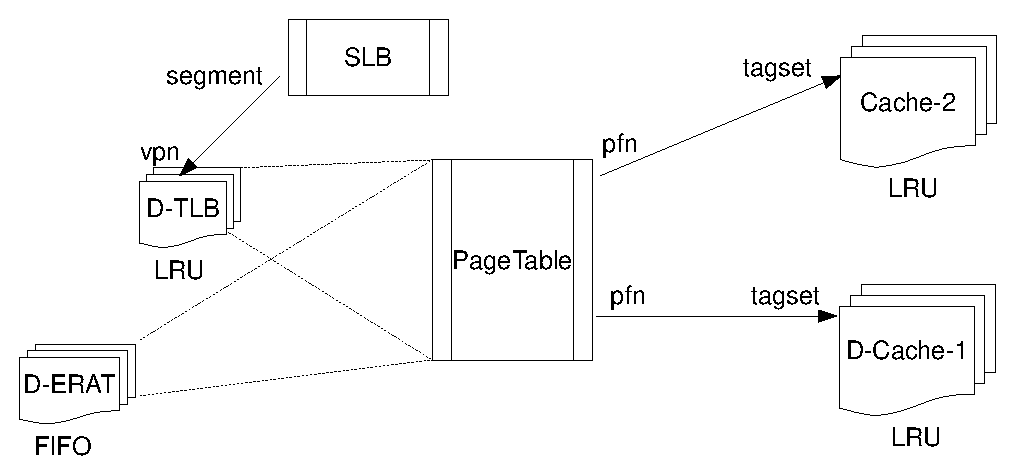
\includegraphics[width=0.8\textwidth]{4.analysis/ppc}\\
  \caption{����� MMU ��������������� PowerPC 970FX}\label{powerpc_mmu_scheme}
\end{figure}

���������� ��������� �������� (��. ���.~\ref{powerpc_mmu_scheme}):
\begin{itemize}
  \item �� ������� D-ERAT--���-������, ��� ��� ���������� �� D-ERAT �����
����������� ����� (pfn) ���������� ������� ����� ������� �����������
������;
  \item �� ������� SLB--D-TLB, ��� ��� �������� ����������� ��������
  ���������� ������� ����� ������ �������� ����������� ������ (vpn);
  \item �� ������� D-TLB--���-������, ��� ��� ���������� �� D-TLB �����
����������� ����� (pfn) ���������� ������� ����� ������� �����������
������.
\end{itemize}

\section{��������� ����������� ��� ����������� Alpha}

\begin{utv}
��� ����������� Alpha �������� ���������� ���������� �������
��������� �����������, ����������� � �����������, ��� ���������
�������� �������� �� �������� ��������.
\end{utv}

���������� ���������� ���������� ��������� � ������ �
��������������� ����������� Alpha. MMU � ���������������� Alpha
�������� � ����  (�������������� �������������� ��������� ���
��������������� Alpha 21264~\cite{HennessyPatterson3rd} -- ��.
���.~\ref{alpha_mmu_scheme}):
\begin{itemize}
  \item \emph{���-������ ������ ������� ������ (D-Cache-1)}:
  virtually indexed physically tagged, ������ 64 ���������,
  �������-�������������, ���������� ������ ����� 2, ��������� ����������
  \LRU, ������ ������ ���-������ 64 �����;
  \item \emph{���-������ ������� ������ (Cache-2)}: physically
  indexed physically tagged, ������� �����������, ������ �� 1 �� 16
  ��������
  \item \emph{������� TLB (D-TLB)}: 128 �����, ���������
  �������������, ������ ������������ ������ 48/43 ���, ������ ����������� ������
  44/41 ���, ������ �������� ����������� ������ �� 8 �������� �� 4
  ��������;
  \item \emph{����� ����������� ������ (VictimBuffer)}: ���������
  �������������, ���������� ����� ����� 8, ���������
  ���������� \FIFO.
\end{itemize}
����� �������, �������� �������� ��� ������ ����������� -- �������
������ ����������� ���-������.

���������� ����� ��������� �������� �������� �:
\begin{itemize}
  \item ���-������ ������ ������� ������;
  \item ���-������ ������� � ������� �������.
\end{itemize}

\begin{figure}[h] \center
  \includegraphics[width=0.8\textwidth]{4.analysis/alpha}\\
  \caption{����� MMU ��������������� Alpha}\label{alpha_mmu_scheme}
\end{figure}

���������� ��������� �������� �� ������� TLB--���-������, ��� ���
���������� �� TLB ����� ����������� ����� (pfn) ���������� �������
����� ������� ����������� ������ (��.���.~\ref{alpha_mmu_scheme}).



\section{��������� ����������� ��� ����������� Pentium}

\begin{utv}
��� ����������� Pentium �������� ���������� ���������� �������
��������� �����������, ����������� � �����������, ��� ���������
�������� �������� �� �������� ��������.
\end{utv}

���������� ���������� ���������� ��������� � ������ �
��������������� ����������� Pentium P6. MMU � ����������������
Pentium �������� � ���� (�������������� �������������� ��������� ���
��������������� Intel Pentium III~\cite{HennessyPatterson3rd} -- ��.
���.~\ref{p6_mmu_scheme}):
\begin{itemize}
  \item \emph{���-������ ������ ������� ������ (D-Cache-1)}: ������
  16 ��������, �������-�������������, ���������� ������ ����� 2,
  ��������� ���������� \LRU, ������ ������ 32 �����;
  \item \emph{���-������ ������� ������ (Cache-2)}: ������ �� 256 ��������
  �� 2 ��������, �������-�������������, ���������� ������ ����� 8, ���������
  ���������� \LRU, ������ ������ 32 �����;
  \item \emph{���-����� TLB (D-TLB)}: �������-�������������,
  ���������� ������ ����� 4, � ������ ������ 16 �����, ��������� ����������
  \PseudoLRU;
  \item \emph{������� ������� ����������� ������ (PageTable)}:
  ������ �������� �� 8 ��������, ����� ����������� ������ 48 ���,
  ����� ��������� ������ 32 ����, ����� ����������� ������ 32 ����;
  \item \emph{������� ������������ ��������� (SDT)}: ������ �� 8 ���� �� 64
  ��������~\cite{FundamentalOfComputerOrganizationAndDesign}.
\end{itemize}
����� �������, �������� ��������� ��� ������ ����������� ��
���-������ � �� TLB.

���������� ����� ��������� �������� �������� �:
\begin{itemize}
  \item ���-������ ������ ������� ������, ������� � ������� �������;
  \item ���-������ ������ TLB (D-TLB).
\end{itemize}

\begin{figure}[h] \center
  \includegraphics[width=0.8\textwidth]{4.analysis/p6}\\
  \caption{����� MMU ��������������� Pentium}\label{p6_mmu_scheme}
\end{figure}

���������� ��������� �������� (��. ���.~\ref{p6_mmu_scheme}):
\begin{itemize}
  \item �� ������� SDT--D-TLB, ��� ��� �������� ����������� ��������
  ���������� ������� ����� ������ �������� ����������� ������ (vpn);
  \item �� ������� D-TLB--���-������, ��� ��� ���������� �� D-TLB �����
����������� ����� (pfn) ���������� ������� ����� ������� �����������
������;
  \item �� ������� SDT--���-������ ��� �������������� ���������, ��� ���
  ���������� �� SDT ���������� ������� ���������� ������� ����� ������� �����������
������.
\end{itemize}


%! добавить еще результаты экспериментов! :)

% !Mode:: "TeX:UTF-8"
\chapter*{Заключение}
\addcontentsline{toc}{chapter}{Заключение}

Основные научные и практические результаты, полученные в
диссертационной работе и выносимые на защиту, состоят в следующем:

\Results

%Основные результаты диссертации являются новыми, получены автором самостоятельно.




\pagebreak
\appendix
% % !Mode:: "TeX:UTF-8"
\chapter{Таблицы ограничений}
%\addcontentsline{toc}{chapter}{Приложение А: Таблицы ограничений}

\begin{table}[h] \small
\begin{tabular}{|c|c|c|c|}
\hline  & \centering случай &
\begin{tabular}{c}переменная\\перебора\end{tabular} & система \\
\hline \hline \multirow{10}{*}{\rotatebox{90}{кэш-попадание}} &
\makecell[c{p{0.3\textwidth}}]{тегсет находится в начальном
состоянии буфера, к нему нет обращений до данной инструкции и он всё
ещё не вытеснен} & $\lambda \in L_0$ &
$\left\{\begin{array}{l} x = \lambda\\
x \notin \{x_1, ..., x_n\}\\
\bigwedge\limits_{x_m:\mbox{miss}}\sum\limits_{i=1}^W v_m(\xi_i) +
\sum\limits^{m-1}_{i=1} u_m(x_i) < W
\end{array}\right.
$ \\ \hhline{~|---} & \makecell[c{p{0.3\textwidth}}]{тегсет
находится в начальном состоянии буфера, к нему есть обращение до
данной инструкции и он всё ещё не вытеснен} & $\lambda \in L_0$ &
$\left\{\begin{array}{l} x = \lambda\\
x \in \{x_1, ..., x_n\}\\
\bigwedge\limits_{x_m:\mbox{miss}}\sum\limits^{m-1}_{i=1} u_m(x_i) <
W
\end{array}\right.
$ \\  \hhline{~|---} & \makecell[c{p{0.3\textwidth}}]{тегсет был
внесен одним из кэш-промахов и с того момента не вытеснен} & -- &
$\left\{\begin{array}{l}
x \in [x_1, ..., x_n]_{miss}\\
\bigwedge\limits_{x_m:\mbox{miss}}\sum\limits^{m-1}_{i=1} u_m(x_i) <
W
\end{array}\right.
$ \\ \hline \hline \multirow{20}{*}{\rotatebox{90}{кэш-промах}} &
\makecell[c{p{0.3\textwidth}}]{тегсет встречается впервые} & -- &
$\left\{\begin{array}{l} x \notin L_0\\
x \notin [x_1, ..., x_n]_{miss}\\
\end{array}\right.
$ \\ \hhline{~|---} & \makecell[c{p{0.3\textwidth}}]{тегсет ранее
был внесен одной из инструкций шаблона, затем вытеснен} & -- &
$\left\{\begin{array}{l}
x \in [x_1, ..., x_n]_{miss}\\
\bigvee\limits_{x_m : \mbox{miss}}\sum\limits^{m-1}_{i=1} u_m(x_i) \geqslant W\\
\end{array}\right.$ \\  \hhline{~|---} &
\makecell[c{p{0.3\textwidth}}]{тегсет находился в начальном
состоянии буфера и был вытеснен, к нему не было обращений в шаблоне}
& $\lambda \in L_0$ & $\left\{\begin{array}{l}
x = \lambda\\
x \notin \{x_1, ..., x_n\}\\
\bigvee\limits_{x_m : \mbox{miss}}\sum\limits^W_{i=1} v_m(\xi_i) + \sum\limits^{m-1}_{i=1} u_m(x_i) \geqslant W\\
\end{array}\right.
$ \\ \hhline{~|---} & \makecell[c{p{0.3\textwidth}}]{тегсет
находился в начальном состоянии буфера и был вытеснен, к нему было
обращение в шаблоне после последнего внесения в буфер} & $\lambda
\in L_0$ &
$\left\{\begin{array}{l} x = \lambda\\
x \in \{x_1, ..., x_n\}\\
\bigvee\limits_{x_m : \mbox{miss}}\sum\limits^{m-1}_{i=1} u_m(x_i) \geqslant W\\
\end{array}\right.
$ \\ \hline
\end{tabular}
\caption{Таблица систем уравнений в случае стратегии вытеснения
\PseudoLRU c использованием функций полезности}\label{plru_table}
\end{table}


\begin{landscape}
\begin{table}[p]\small
\begin{tabular}{|c|c|c|c|c|c|}
\hline  & \centering случай &
\begin{tabular}{c}переменная\\перебора\end{tabular} & система &
\begin{tabular}{c}функция полезности\\для кэш-попадания\end{tabular} &
\begin{tabular}{c}функция полезности\\для кэш-промаха\end{tabular} \\
\hline \hline \multirow{10}{*}{\rotatebox{90}{кэш-попадание}} &
\makecell[c{p{0.38\textwidth}}]{тегсет находится в начальном
состоянии буфера, к нему нет обращений до данной инструкции и он всё
ещё не вытеснен} & $\lambda_\delta \in D$ &
$\left\{\begin{array}{l} x = \lambda_\delta\\
x \notin \{x_1, ..., x_n\}\\
\sum\limits^n_{i=1} u(x_i) \leqslant w - \delta
\end{array}\right.
$ &
\begin{tabular}{c}
$x_i \in \{ \lambda_{\delta+1}, ..., \lambda_w\}$\\
$\wedge~x_i \notin \{x_1, ..., x_{i-1}\}$
\end{tabular}
& $R(x_i) = R(x)$
\\ \hhline{~|-----}
& \makecell[c{p{0.38\textwidth}}]{тегсет находится в начальном
состоянии буфера, к нему есть обращение до данной инструкции и он
всё ещё не вытеснен} & $\lambda_\delta \in D$ &
$\left\{\begin{array}{l} x = \lambda_\delta\\
x \in \{x_1, ..., x_n\}\\
\sum\limits^n_{i=1} u(x_i) < w
\end{array}\right.
$ &
\begin{tabular}{c}
$x \notin \{x_i, ..., x_n\}~\wedge$\\
$x_i \in \{ \lambda_{\delta+1}, ..., \lambda_w\}$\\
$\wedge~x_i \notin \{ x_{i+1}, ..., x_n\}$\\
\end{tabular}
&
\begin{tabular}{c}
$x \notin \{x_i, ..., x_n\}$\\
$\wedge~R(x_i) = R(x)$\\
\end{tabular}
\\  \hhline{~|-----}
& \makecell[c{p{0.38\textwidth}}]{тегсет был внесен одним из
кэш-промахов и с того момента не вытеснен} & -- &
$\left\{\begin{array}{l} x \in [x_1, ..., x_n]_{miss}\\
\sum\limits^n_{i=1} u(x_i) < w
\end{array}\right.
$ &
\begin{tabular}{c}
$x \notin \{x_i, ..., x_n\}$\\
$\wedge~R(x_i) = R(x)~\wedge$\\
$x_i \notin \{ x_{i+1}, ..., x_n\}$\\
\end{tabular}
&
\begin{tabular}{c}
$x \notin \{x_i, ..., x_n\}$\\
$\wedge~R(x_i) = R(x)$\\
\end{tabular}
\\ \hline \hline \multirow{15}{*}{\rotatebox{90}{кэш-промах}}
& \makecell[l]{тегсет встречается впервые} & -- &
$\left\{\begin{array}{l} x \notin D\\
x \notin [x_1, ..., x_n]_{miss}\\
\end{array}\right.
$ & -- & -- \\ \hhline{~|-----} &
\makecell[l{p{0.38\textwidth}}]{тегсет ранее был внесен одной из
инструкций шаблона, затем вытеснен} & -- & $\left\{\begin{array}{l}
x \in [x_1, ..., x_n]_{miss}\\
\sum\limits^n_{i=1} u(x_i) \geqslant w\\
\end{array}\right.$ &
\begin{tabular}{c}
$x \notin \{x_i, ..., x_n\}$\\
$\wedge~R(x_i) = R(x)~\wedge$\\
$x_i \notin \{ x_{i+1}, ..., x_n\}$\\
\end{tabular}
&
\begin{tabular}{c}
$x \notin \{x_i, ..., x_n\}$\\
$\wedge~R(x_i) = R(x)$\\
\end{tabular}
\\  \hhline{~|-----} &
\makecell[c{p{0.38\textwidth}}]{тегсет находился в начальном
состоянии буфера и был вытеснен, к нему не было обращений в шаблоне}
& $\lambda_\delta \in D$ &
$\left\{\begin{array}{l} x = \lambda_\delta\\
x \notin \{x_1, ..., x_n\}\\
\sum^n_{i=1} u(x_i) \geqslant w - \delta + 1\\
\end{array}\right.
$ &
\begin{tabular}{c}
$x_i \in\{\lambda_{\delta+1}, ..., \lambda_w\}$\\
$\wedge~x_i \notin \{x_1, ..., x_{i-1}\}$\\
\end{tabular}
&
\begin{tabular}{c}
$R(x_i) = R(x)$\\
\end{tabular}
\\ \hhline{~|-----} &
\makecell[c{p{0.38\textwidth}}]{тегсет находился в начальном
состоянии буфера и был вытеснен, к нему было обращение в шаблоне
после последнего внесения в буфер} & $\lambda_\delta \in D$ &
$\left\{\begin{array}{l} x = \lambda_\delta\\
x \in \{x_1, ..., x_n\}\\
\sum\limits^n_{i=1} u(x_i) \geqslant w\\
\end{array}\right.
$ &
\begin{tabular}{c}
$x \notin \{x_i, ..., x_n\}~\wedge$\\
$x_i \in \{\lambda_{\delta+1}, ..., \lambda_w\}$\\
$\wedge x_i \notin \{ x_{i+1}, ..., x_n\}$\\
\end{tabular}
&
\begin{tabular}{c}
$x \notin \{x_i, ..., x_n\}$\\
$\wedge~R(x_i) = R(x)$\\
\end{tabular}
\\ \hline
\end{tabular}
\caption{Таблица систем уравнений для тестовых ситуаций в \LRU
кэширующих буферах c использованием функций
полезности}\label{hit_miss_table}
\end{table}
\end{landscape}

\begin{landscape}
\begin{table}
\begin{tabular}{|c|c|c|c|c|c|}
\hline  & \centering случай &
\begin{tabular}{c}переменная\\перебора\end{tabular} & система &
\begin{tabular}{c}функция\\полезности\\для кэш-\\попадания\end{tabular} &
\begin{tabular}{c}функция\\полезности\\для кэш-\\промаха\end{tabular} \\
\hline \hline \rotatebox{90}{кэш-попадание} & -- & -- & -- & -- & --
\\ \hline \hline \multirow{15}{*}{\rotatebox{90}{кэш-промах}} &
\makecell[c{p{0.35\textwidth}}]{тегсет встречается впервые} & -- &
$\left\{\begin{array}{l} x \notin D\\
x \notin [x_1, ..., x_n]_{miss}\\
\end{array}\right.
$ & -- & -- \\ \hhline{~|-----} &
\makecell[c{p{0.35\textwidth}}]{тегсет ранее был внесен одной из
инструкций шаблона, затем вытеснен} & -- & $\left\{\begin{array}{l}
x \in [x_1, ..., x_n]_{miss}\\
\left[ \sum\limits^n_{i=1} \right]_{miss} u(x_i) \geqslant w - \delta + 1\\
\end{array}\right.$& -- &
\begin{tabular}{c}
$x \notin \{x_i, ..., x_n\}$\\
$\wedge~R(x_i) = R(x)$\\
\end{tabular}
\\  \hhline{~|-----} &
\makecell[c{p{0.35\textwidth}}]{тегсет находился в начальном
состоянии буфера и был вытеснен, к нему не было обращений в шаблоне}
& $\lambda_\delta \in D$ &
$\left\{\begin{array}{l} x = \lambda_\delta\\
x \notin \{x_1, ..., x_n\}\\
\left[ \sum\limits^n_{i=1} \right]_{miss} u(x_i) \geqslant w - \delta + 1\\
\end{array}\right.$ & -- &
\begin{tabular}{c}
$R(x_i) = R(x)$\\
\end{tabular}
\\ \hhline{~|-----} &
\makecell[c{p{0.35\textwidth}}]{тегсет находился в начальном
состоянии буфера и был вытеснен, к нему было обращение в шаблоне
после последнего внесения в буфер} & $\lambda_\delta \in D$ &
$\left\{\begin{array}{l} x = \lambda_\delta\\
x \in \{x_1, ..., x_n\}\\
\left[ \sum\limits^n_{i=1} \right]_{miss} u(x_i) \geqslant w\\
\end{array}\right.$ & -- &
\begin{tabular}{c}
$x \notin \{x_i, ..., x_n\}$\\
$\wedge~R(x_i) = R(x)$\\
\end{tabular}
\\ \hline
\end{tabular}
\caption{Таблица систем ограничений в случае стратегии вытеснения
\FIFO c использованием функций полезности}\label{fifo_table}
\end{table}
\end{landscape}

\begin{landscape}
\begin{table} \small
\begin{tabular}{|c|c|c|c|c|c|}
\hline  & \centering случай &
\begin{tabular}{c}переменная\\перебора\end{tabular} & система &
\begin{tabular}{c}функция полезности\\для кэш-попадания\end{tabular} &
\begin{tabular}{c}функция полезности\\для кэш-промаха\end{tabular} \\
\hline \hline \multirow{10}{*}{\rotatebox{90}{кэш-попадание}} &
\makecell[c{p{0.38\textwidth}}]{тегсет находится в начальном
состоянии буфера, к нему нет обращений до данной инструкции и он всё
ещё не вытеснен} & $\lambda_\delta \in D$ &
$\left\{\begin{array}{l} x = \lambda_\delta\\
x \notin \{x_1, ..., x_n\}\\
\sum\limits^n_{i=1} u(x_i) \leqslant w - \delta
\end{array}\right.
$ &
\begin{tabular}{c}
$x_i \in \{ \lambda_{\delta+1}, ..., \lambda_\Delta\}$\\
$\wedge~x_i \notin \{x_1, ..., x_{i-1}\}$
\end{tabular}
& $R(x_i) = R(x)$
\\ \hhline{~|-----}
& \makecell[c{p{0.38\textwidth}}]{тегсет находится в начальном
состоянии буфера, к нему есть обращение до данной инструкции и он
всё ещё не вытеснен} & $\lambda_\delta \in D$ &
$\left\{\begin{array}{l} x = \lambda_\delta\\
x \in \{x_1, ..., x_n\}\\
\sum\limits^n_{i=1} u(x_i) < w
\end{array}\right.
$ &
\begin{tabular}{c}
$x \notin \{x_i, ..., x_n\}~\wedge$\\
$x_i \in \{ \lambda_{\delta+1}, ..., \lambda_\Delta\}$\\
$\wedge~x_i \notin \{ x_{i+1}, ..., x_n\}$\\
\end{tabular}
&
\begin{tabular}{c}
$x \notin \{x_i, ..., x_n\}$\\
$\wedge~R(x_i) = R(x)$\\
\end{tabular}
\\  \hhline{~|-----}
& \makecell[c{p{0.38\textwidth}}]{тегсет был внесен одним из
кэш-промахов и с того момента не вытеснен} & -- &
$\left\{\begin{array}{l} x \in [x_1, ..., x_n]_{miss}\\
\sum\limits^n_{i=1} u(x_i) < w
\end{array}\right.
$ &
\begin{tabular}{c}
$x \notin \{x_i, ..., x_n\}$\\
$\wedge~R(x_i) = R(x)~\wedge$\\
$x_i \notin \{ x_{i+1}, ..., x_n\}$\\
\end{tabular}
&
\begin{tabular}{c}
$x \notin \{x_i, ..., x_n\}$\\
$\wedge~R(x_i) = R(x)$\\
\end{tabular}
\\ \hline \hline \multirow{20}{*}{\rotatebox{90}{кэш-промах}}
& \makecell[c{p{0.38\textwidth}}]{тегсет встречается впервые} & -- &
$\left\{\begin{array}{l} x \notin D\\
x \notin [x_1, ..., x_n]_{miss}\\
\end{array}\right.
$ & -- & -- \\ \hhline{~|-----} &
\makecell[c{p{0.38\textwidth}}]{тегсет ранее был внесен одной из
инструкций шаблона, затем вытеснен} & -- &
$\left\{\begin{array}{l} x \in [x_1, ..., x_n]_{miss}\\
\sum\limits^n_{i=1} u(x_i) \geqslant w\\
\end{array}\right.
$ &
\begin{tabular}{c}
$x \notin \{x_i, ..., x_n\}$\\
$\wedge~R(x_i) = R(x)~\wedge$\\
$x_i \notin \{ x_{i+1}, ..., x_n\}$\\
\end{tabular}
&
\begin{tabular}{c}
$x \notin \{x_i, ..., x_n\}$\\
$\wedge~R(x_i) = R(x)$\\
\end{tabular}
\\  \hhline{~|-----} &
\makecell[c{p{0.38\textwidth}}]{тегсет находился в начальном
состоянии буфера и был вытеснен, к нему не было обращений в шаблоне}
& $\lambda_\delta \in D$ &
$\left\{\begin{array}{l} x = \lambda_\delta\\
x \notin \{x_1, ..., x_n\}\\
\sum\limits^n_{i=1} u(x_i) \geqslant w - \delta + 1\\
\end{array}\right.
$ &
\begin{tabular}{c}
$x_i \in\{\lambda_{\delta+1}, ..., \lambda_\Delta\}$\\
$\wedge~x_i \notin \{x_1, ..., x_{i-1}\}$\\
\end{tabular}
&
\begin{tabular}{c}
$R(x_i) = R(x)$\\
\end{tabular}
\\ \hhline{~|-----} &
\makecell[c{p{0.38\textwidth}}]{тегсет находился в начальном
состоянии буфера и был вытеснен, к нему было обращение в шаблоне
после последнего внесения в буфер} & $\lambda_\delta \in D$ &
$\left\{\begin{array}{l} x = \lambda_\delta\\
x \in \{x_1, ..., x_n\}\\
\sum\limits^n_{i=1} u(x_i) \geqslant w\\
\end{array}\right.
$ &
\begin{tabular}{c}
$x \notin \{x_i, ..., x_n\}~\wedge$\\
$x_i \in \{\lambda_{\delta+1}, ..., \lambda_\Delta\}$\\
$\wedge~x_i \notin \{ x_{i+1}, ..., x_n\}$\\
\end{tabular}
&
\begin{tabular}{c}
$x \notin \{x_i, ..., x_n\}$\\
$\wedge~R(x_i) = R(x)$\\
\end{tabular}
\\ \hline
\end{tabular}
\caption{Таблица систем уравнений для тестовых ситуаций в \LRU
кэширующем буфере c <<грязными>> ячейками в начальном состоянии,
использующих функции полезности}\label{dirty_hit_miss_table}
\end{table}
\end{landscape}

%TODO!!! % !Mode:: "TeX:UTF-8"
\chapter{Доказательства теорем и лемм}\label{sec:proofs}
%\addcontentsline{toc}{chapter}{Приложение А: Таблицы ограничений}

\theoremtext{\ref{mirror_fullness_none}}{\FullnessMirrorNone}
\begin{proof}
  Особо подчеркну сначала, что в формулировке теоремы $n$ --- количество обращений к таблице в тестовом шаблоне. А в алгоритме построения ограничений $n$ --- количество \textbf{успешных} обращений к таблице в тестовом шаблоне. Чтобы согласовать обозначения, будем далее придерживаться обозначений из алгоритма: ключи в регионах с успешными обращениями обозначать как $k_i$, $R_i$ для $i = 1, 2, ..., n$, а ключа в регионах с неуспешными обращениями обозначать как $k'_j$, $R'_j$ для $j = 1, 2, ..., n'$ ($n$ в формулировке теоремы есть новое $n$ + $n'$).
  
  Обозначим $L$ --- состояние таблицы перед тестовым шаблоном. Тогда согласно посылке в условии теоремы для каждого допустимого $i$ выполнено: $(k_i || R_i) \in L$ --- и для каждого допустимого $j$ выполнено: $(k'_j || R'_j) \notin L$. Для всех инструкций состояние таблицы одно и то же, поскольку стратегия вытеснения есть \texttt{none} (промах лишь фиксируется, но не <<исправляется>>). Тем самым. $L \supseteq \{ (k_1||R_1), ..., (k_n||R_n) \}$. Отсюда следует, что для каждого допустимого $j$ $(k'_j||R'_j) \notin \{ (k_1||R_1), ..., (k_n||R_n) \}$.
  
  Кроме того, поскольку $L$ --- состояние таблицы перед тестовым шаблоном, то количество ключей в каждом регионе, которое может находиться в $L$ равно $w$ (по определению $w$). Но поскольку $L \supseteq \{ (k_1||R_1), ..., (k_n||R_n) \}$, то количество различных ключей в каждом регионе в последовательности $(k_i, R_i)$ не может быть больше $w$. Осталось показать, что это количество выражается формулой, представленной в алгоритме. Действительно, для получения количества различных ключей в том же регионе достаточно просматривать все ключи с начала и отсчитывать те из них, что встречаются впервые, т.е. не встречаются среди предыдущих ключей, что и выражено в формуле.
  
  Итак, если для щаблона в заданном начальном состоянии есть какая-нибудь последовательность ключей в регионах, то система ограничений будет совместна, поскольку на этих же ключах и регионах выполнены ограничения, генерируемые согласно алгоритму.
\end{proof}

\theoremtext{\ref{mirror_fullness}}{\FullnessMirror}
\begin{proof}
Докажем даже более сильное утверждение (из него очевидно будет следовать требуемое в теореме): есть начальное состояние таблицы $L_0$, для него существуют такие $k_1, k_2, ..., k_n$, $R_1, R_2, ..., R_n$, что выполнены все $S_i$ и $P$; спрашивается, будут ли существовать такие $t_1, t_2, ..., t_m$, $r_1, r_2, ..., r_m$, что составленные ограничения (для тех же $k_1, k_2, ..., k_n$, $R_1$, $R_2$, ..., $R_n$) будут выполнены. Весь вопрос в том, как выбрать $t_1, t_2, ..., t_m$, $r_1, r_2, ..., r_m$. Доказательство можно разделить на две части: в первой будет предложен способ выбора $t_1, t_2, ..., t_m$, $r_1, r_2, ..., r_m$, а во второй будет показано, что на них выполняются ограничения.

\paragraph{выбор инициализирующей последовательности} предлагается делать\\следующим образом. Она будет состоять из подпоследовательностей $s_R$ для каждого $R$ из \textbf{множества} $\{R_1, R_2, ..., R_n\}$. Далее рассматривается построение такой подпоследовательности для произвольного $R$. Выберем из $L_0$ ключи, хранящиеся в регионе $R$, ровно в том порядке, в каком они там находятся (речь идет о порядке в смысле перестановок в таблицах вытеснения). Обозначим эту последовательность $V \equiv \langle v_1, v_2, ..., v_q \rangle$. Далее, удалим из последовательности $k_1, k_2, ..., k_n$ те ключи, чьи регионы не равны $R$, и те, которые присутствуют в последовательности $v_1, v_2, ..., v_q$. Обозначим получившуюся последовательность $U \equiv \langle u_1, u_2, ..., u_p\rangle$. Если $p < w$, то выберем $p{-}w$ произвольных ключей, не встречающихся в последовательностях $U$ и $V$. Обозначим эту последовательность $Z$. Тогда $s_R$ будет являться конкатенацией последовательностей $Z$, $U$ и $V$ (именно в этом порядке). Порядок конкатенации последовательностей $s_R$ произвольный. Последовательность $r_1, r_2, ..., r_m$ выбирается в соответствии с выбором последовательности конкатенации $s_R$.

\paragraph{выполнение системы ограничений} По построению все $(t_1||r_1)$, $(t_2||r_2)$, ..., $(t_m||r_m)$ разные. Кроме того, поскольку на $(k_i, R_i)$ выполнены все условия в тестовом шаблоне, то для них выполнено условие количества различных пар (ключ, регион) в каждом регионе для каждой инструкции. Далее, поскольку последовательность $(t_i, r_i)$ оканчивается последовательностью, дублирующей $L_0$ и стратегия вытеснения является существенно вытесняющей, то после таких инициализирующих обращений состояние таблиц станет точно таким же, каким оно было до инициализирующих обращений. Это значит, что для $(k_i, R_i)$ выполнены ограничения <<быть вытесненным>> (они и есть $S_i$). И поскольку последовательность $(t_1, r_1)$, $(t_2, r_2)$, .., $(t_m, r_m)$ содержит все $(k_1, R_1)$, ..., $(k_n, R_n)$, то выполнены ограничения\\$(k_i||R_i) \in \{(t_1||r_1), (t_2||r_2), ..., (t_m||r_m), (k_1||R_1), (k_2||R_2), ..., (k_{i-1}||R_{i-1})\}$.
\end{proof}

\begin{lemma}\label{PseudoLRUNolDisplacing}
Рассматривается последовательность промахов при стратегии вытеснения \PseudoLRU. Тогда в результате $w{-}1$ промаха строка региона на позиции 0 не будет вытеснена.
\end{lemma}
\begin{proof}
    Доказательство для лучшей читабельности приведено для случая $w = 8$, хотя всё аналогичное переносится на случай произвольного $w = 2^W$.

    Последняя строка таблицы вытеснения для \PseudoLRU имеет вид:\\$(m~6~4~5~0~1~2~3)$. Если разложить каждую позицию в битовую строку, то эту же перестановку можно задать следующим образом:
    \begin{itemize}
        \item элемент с позиции $x \in \{\bigl(\begin{smallmatrix}0\\0\\0
\end{smallmatrix}\bigr), \bigl(\begin{smallmatrix}0\\0\\1
\end{smallmatrix}\bigr), \bigl(\begin{smallmatrix}0\\1\\0
\end{smallmatrix}\bigr), \bigl(\begin{smallmatrix}0\\1\\1
\end{smallmatrix}\bigr)\}$ перемещается на позицию $x \oplus \bigl(\begin{smallmatrix}1\\0\\0
\end{smallmatrix}\bigr)$;
        \item элемент с позиции $x \in \{\bigl(\begin{smallmatrix}1\\0\\0
\end{smallmatrix}\bigr), \bigl(\begin{smallmatrix}1\\0\\1
\end{smallmatrix}\bigr)\}$ перемещается на позицию $x \oplus \bigl(\begin{smallmatrix}1\\1\\0
\end{smallmatrix}\bigr)$;
        \item элемент с позиции $x \in \{\bigl(\begin{smallmatrix}1\\1\\0
\end{smallmatrix}\bigr)\}$ перемещается на позицию $x \oplus \bigl(\begin{smallmatrix}1\\1\\1
\end{smallmatrix}\bigr)$;
        \item $m$ помещается на позицию 0.
\end{itemize}

Сокращая обозначения, перефразируем это:
\begin{itemize}
    \item элемент с позиции $x = \bigl(\begin{smallmatrix}0\\X\\X\end{smallmatrix}\bigr)$ перемещается на позицию $x \oplus \bigl(\begin{smallmatrix}1\\0\\0 \end{smallmatrix}\bigr)$;
    \item элемент с позиции $x = \bigl(\begin{smallmatrix}1\\0\\X\end{smallmatrix}\bigr)$ перемещается на позицию $x \oplus \bigl(\begin{smallmatrix}1\\1\\0\end{smallmatrix}\bigr)$;
    \item элемент с позиции $x = \bigl(\begin{smallmatrix}1\\1\\0\end{smallmatrix}\bigr)$ перемещается на позицию $x \oplus \bigl(\begin{smallmatrix}1\\1\\1\end{smallmatrix}\bigr)$;
    \item $m$ помещается на позицию 0.
\end{itemize}

Перевернем каждый столбец. Получится следующий набор правил перемещения в результате промаха:
\begin{itemize}
    \item элемент с позиции $x = \bigl(\begin{smallmatrix}X\\X\\0\end{smallmatrix}\bigr)$ перемещается на позицию $x \oplus \bigl(\begin{smallmatrix}0\\0\\1 \end{smallmatrix}\bigr)$;
    \item элемент с позиции $x = \bigl(\begin{smallmatrix}X\\0\\1\end{smallmatrix}\bigr)$ перемещается на позицию $x \oplus \bigl(\begin{smallmatrix}0\\1\\1\end{smallmatrix}\bigr)$;
    \item элемент с позиции $x = \bigl(\begin{smallmatrix}0\\1\\1\end{smallmatrix}\bigr)$ перемещается на позицию $x \oplus \bigl(\begin{smallmatrix}1\\1\\1\end{smallmatrix}\bigr)$;
    \item $m$ помещается на позицию 0.
\end{itemize}

Под действием этих правил происходят $w{-}1$ перемещений с <<перевернутой>> позиции $\bigl(\begin{smallmatrix}0\\0\\0\end{smallmatrix}\bigr)$. Покажем, что это перемещение имеет очень простой вид: 0, 1, 2, ... . Докажем по индукции. База очевидна: позиция изначально равна 0. Индуктивный переход. За позицией $2k$ будет следовать позиция $2k+1$ под действием первого правила. За позицией $2k+1$ будет следовать позиция $2k+2$ под действием остальных правил (0 и последовательность единичных битов инвертируется, что и есть прибавление единицы).

А если перемещение имеет такой вид, то за $w{-}1$ перемещение ни одна из <<перевернутых>> позиций (а, значит, и просто позиций) не равна $w{-}1$ (0, 1, 2, ..., $w{-}2$). А позиция $w{-}1$ --- это и есть позиция вытеснения согласно последней строке таблицы вытеснения для \PseudoLRU.
\end{proof}

\theoremtext{\ref{thm:PseudoLRU_essential}}{\PseudoLRUEssential}
\begin{proof}
    Из леммы~\ref{PseudoLRUNolDisplacing} следует, что первый внесенный в результате промаха $m$ не будет вытеснен после $w{-}1$ промахов. Однако при каждом промахе какие-то элементы вытесняются. Вносимые на каждом промахе $m$ проходят ту же <<траекторию>>, что и первый. Поэтому к ним снова применима лемма~\ref{PseudoLRUNolDisplacing}. Тем самым после $w$ промахов в регионе будет $w$ штук $m$. Но больше, чем $w$, и не может быть, поскольку это количество строк в регионе. Значит, после $w$ промахов весь регион будет состоять лишь из одних $m$.
\end{proof}

\theoremtext{\ref{thm_mirror_lenth_lru}}{\UpperBoundLRUMirror}
\begin{proof}
  Так же, как это было сделано при доказательстве
  теоремы~\ref{mirror_fullness}, разделим все $k_1, k_2, ..., k_n$
  по регионам. Для каждого задействованного региона составим свою
  инициализирующую последовательность (обозначим ее длину $m_i$
  для $i$'го задействованного региона) и сконкатенируем эти
  последовательности для получения искомой инициализирующей последовательности
   для всего тестового шаблона.
  Подпоследовательность последовательности $k_1, k_2, ..., k_n$,
  соответствующая одному региону, обозначим $y_1, y_2, ...,
  y_{n_i}$.

  Докажем, что $$m_i = M_i + w$$ где $M_i$ -- количество
  элементов последовательности $y_1, y_2, ..., y_{n_i}$, которые дают
  промахи при первых обращениях к ним. Тогда для всего тестового
  шаблона $m = \sum\limits_i m_i = \sum\limits_i M_i + \sum\limits_i w =
  M + w \cdot r$, где $r$ -- количество регионов, задействованных в
  $k_1, k_2, ..., k_n$. Очевидно, что $r \leqslant n$, тем самым это
  приводит к искомой оценке $m \leqslant M + n \cdot w$. Осталось
  доказать формулу для $m_i$.

  Укажем способ построения ключей инициализирующей последовательности. Выберем из $y_1, y_2, ..., y_{n_i}$ подпоследовательность,
  состоящую из тех ключей, которые дают промах и встречаются
  впервые. Обозначим их как $\mu \equiv \mu_1, \mu_2, ..., \mu_{MM_i}$. Они будут первыми ключами в   инициализирующей последовательности. Далее выберем из $y_1, y_2, ..., y_{n_i}$
  все ключи, при обращении к которым происходят попадания.
  Обозначим их как $\eta \equiv \eta_1, \eta_2, ..., \eta_{HH_i}$. Если $MM_i > 0$ и $MM_i +
  HH_i < w + 1$, выберем произвольные различные числа-ключи $\nu \equiv \nu_1, \nu_2,
  ..., \nu_{NN_i}$, которые не встречаются в $y_1, y_2, ..., y_{n_i}$. Итак, инициализирующая последовательность (для данного региона!) представляет собой конкатенацию последовательностей $\mu$, $\eta$ и $\nu$ (в этом порядке).

  Покажем, что такая инициализирующая последовательность удовлетворяет системе ограничений. Все ключи из тестового шаблона, при обращении к которым происходят попадания, встречаются в
  этой последовательности. Это следует из того, что первые такие ключи мы поместили явно (в конец последовательности), а дальнейшие ключи не могут встречаться впервые в тестовом шаблоне, в противном случае они были бы вытеснены до того, как должно быть попадание. Очевидно, что эти первые ключи не вытеснены, поскольку они помещены в конец инициализирующей последовательности. Все ключи, при обращении к которыми происходят промахи, тоже встречаются в этой последовательности (мы их туда поместили явно). При этом поскольку от своего промаха они отделены не менее $w+1$ инструкцией с разными ключами, то к моменту промаха они будут
  вытеснены (для первой инструкции это очевидно по построению, а
  для остальных следует из леммы~\ref{includedranges} о невложенных диапазонах вытеснения).

  Длина инициализирующей последовательности для шаблона без промахов (при $MM_i$ = 0) равна количеству ключей в $y_1, y_2, ..., y_{n_i}$, при обращении к
  которым происходят попадания. Их не более чем $w$,
  т.к. последовательность из попаданий может задать лишь часть
  или целиком весь регион. При $MM_i > 0$ длина последовательности
  есть сумма из $M_i$ (поскольку туда включаются все ключи $y_1, y_2,
  ..., y_{n_i}$, при обращении к которым происходят промахи) и
  $w$ (поскольку в инициализирующую последовательность добавляются фиктивные ключи и ключи, при обращении к которым происходят попадания). В обоих случах $m_i = M_i + w$.
\end{proof}

\theoremtext{\ref{thm_pseudoLRU_invariant}}{\PseudoLRUInvariant}
\begin{proof}
  Пусть происходит обращение с позицией $j = (j_1~j_2~\dots~j_W)$.
  Тогда согласно каноническому определению \PseudoLRU будет
  произведены следующие изменения: $B_{(1)} := j_1; B_{(1~j_1)} :=
  j_2; \dots B_{(1~j_1~j_2~\dots~j_{W-1})} := j_W$. Однако только
  часть этих изменений повлияет на
  $(\alpha_1~\alpha_2~\dots~\alpha_W)$, $\alpha_1 = B_{(1)}^{\neg
  i_1}, \alpha_2 = B_{(1~i_1)}^{\neg i_2}, \dots, \alpha_W =
  B_{(1~i_1~i_2~\dots~i_{W-1})}^{\neg i_W}$. А именно влияние будет
  на те элементы вектора, у которых совпадают индексы с изменяемыми
  элементами согласно каноническому определению. Иными словами,
  изменение $B_{(1~j_1~j_2~\dots~j_k)}$ будет влиять на
  $B_{(1~i_1~i_2~\dots~i_m)}$ тогда и только тогда, когда
  $(1~j_1~j_2~\dots~j_k) = (1~i_1~i_2~\dots~i_m)$. Докажем, что при
  этом $k = m$. Действительно, если $k > m$, то
  $(1~j_1~j_2~\dots~j_k) \geqslant 2^k$, а $(1~i_1~i_2~\dots~i_m) <
  2^{m+1} \leqslant 2^k$, что исключает равенство этих чисел.
  Аналогично доказывается невозможность случая $k < m$.

  Условие $(1~j_1~j_2~\dots~j_k) = (1~i_1~i_2~\dots~i_k)$
  эквивалентно условию $(j_1~j_2~\dots~j_k)$ $\oplus~(i_1~i_2~\dots~i_k) =
  0$. Переходя к полным векторам, это условие записывается в виде $(j_1~j_2~\dots~j_W) \oplus
  (i_1~i_2~\dots~i_W) < 2^{W-k+1}$. Или, переходя от векторов к
  числам, $i \oplus j < 2^{W-k+1}$.

  При этом изменение элементов вектора
  ($\alpha_1~\alpha_2~\dots~\alpha_W$) будет происходить следующим
  образом (используется определение степени через сложение по модулю
  2: $x^y \equiv x \oplus y \oplus 1$): $\alpha_k :=
  (B_{(1~j_1~j_2~\dots~j_{k-1})})^{\neg i_k} =
  (B_{(1~j_1~j_2~\dots~j_{k-1})}) \oplus (\neg i_k) \oplus 1 =
  B_{(1~j_1~j_2~\dots~j_{k-1})} \oplus i_k = j_k \oplus i_k$. Так
  как $(j_1~j_2~\dots~j_{k-1}) = (i_1~i_2~\dots~i_{k-1})$, то
  $(j_1~j_2~\dots~j_{k-2}) = (i_1~i_2~\dots~i_{k-2})$ и $i_{k-1} =
  j_{k-1}$. В таком случае изменяется и $\alpha_{k-1}$, причем
  $\alpha_{k-1} := i_{k-1} \oplus j_{k-1} = 0$. Аналогично
  рассуждая, получим, что $\alpha_{k-2} := 0,~\dots~\alpha_1 := 0$.
  Иными словами, возможно даже вычислить изменения предыдущих
  элементов -- всем им присваивается значение 0. Найдется такой $p$,
  что $i_1 = j_1~\wedge~i_2 = j_2~\wedge~i_{p-1} =
  j_{p-1}~\wedge~i_p \neq j_p$. В этом случае изменяется
  $\alpha_p$ следующим образом: $\alpha_p := i_p \oplus j_p = 1$.
  Или записывая это условие с использованием чисел $i$ и $j$: $2^{W-p} \leqslant i
  \oplus j < 2^{W-p+1}$.

  Таким образом, получаем, что для $i \oplus j \in
  [\frac{w}{2^k},~\frac{w}{2^{k-1}})$ будет произведены следующие
  присваивания: $\alpha_k := 1,~\alpha_{k-1} := 0,~\alpha_{k-2} :=
  0,~\dots~\alpha_1 := 0$, остальные элементы не будут изменены. Для
  $i \oplus j = 0$, т.е. $i = j$ все элементы $\alpha_k := i_k \oplus
  j_k = 0$. Причем изменение определяется только суммой по модулю 2
  чисел $i$ и $j$, что и является относительной позицией $j$
  относительно $i$.

  Осталось разобраться с ветвью вытесняемого ключа. Это будет такая
  позиция $i = (i_1~i_2~\dots~i_W)$, для которой справедливы
  уравнения $i_1 = \neg B_{k_1}~\wedge~i_2 = \neg
  B_{k_2}~\wedge~\dots~\wedge~i_W = \neg B_{k_W}$, где $k_1 = (1)$,
  $k_2 = (1~\neg B_{k_1})$, ..., $k_W = (1~\neg B_{k_1}~\neg
  B_{k_2}~\dots\\\neg B_{k_{W-1}})$. Используя уравнения для
  элементов $i$, можно переписать уравнения для элементов $k$
  следующим образом: $k_1 = (1)$,
  $k_2 = (1~i_1)$, ..., $k_W = (1~i_1~i_2~\dots~i_{W-1})$. Таким
  образом, элементы ветви вытесняемого ключа будут вычисляться
  следующим образом: $\alpha_m \equiv B_{(1~i_1~i_2~\dots~i_{m-1})}
  \oplus i_m \equiv B_{k_m} \oplus i_m \equiv \neg i_m \oplus i_m
  \equiv 1$. Иными словами, ветвь вытесняемого ключа состоит только
  из единиц.
\end{proof}


\pagebreak
%%%%\bibliographystyle{plain}
%%%%\bibliographystyle{gost71u}
\addcontentsline{toc}{chapter}{Литература}
\bibliographystyle{gost780s}
\bibliography{thesis}

%% привести оформление в соответствие с требованием: что-то всё время пропадает!

%%! добавить \cite{Pex}, \cite{symbolic_execution}

%%! вписать название препринта и номер тома

\end{document}
